% Options for packages loaded elsewhere
% Options for packages loaded elsewhere
\PassOptionsToPackage{unicode}{hyperref}
\PassOptionsToPackage{hyphens}{url}
%
\documentclass[
  12pt,
]{book}
\usepackage{xcolor}
\usepackage[margin=1in,top=1in,bottom=1in,left=1.5in,right=1in]{geometry}
\usepackage{amsmath,amssymb}
\setcounter{secnumdepth}{5}
\usepackage{iftex}
\ifPDFTeX
  \usepackage[T1]{fontenc}
  \usepackage[utf8]{inputenc}
  \usepackage{textcomp} % provide euro and other symbols
\else % if luatex or xetex
  \usepackage{unicode-math} % this also loads fontspec
  \defaultfontfeatures{Scale=MatchLowercase}
  \defaultfontfeatures[\rmfamily]{Ligatures=TeX,Scale=1}
\fi
\usepackage{lmodern}
\ifPDFTeX\else
  % xetex/luatex font selection
\fi
% Use upquote if available, for straight quotes in verbatim environments
\IfFileExists{upquote.sty}{\usepackage{upquote}}{}
\IfFileExists{microtype.sty}{% use microtype if available
  \usepackage[]{microtype}
  \UseMicrotypeSet[protrusion]{basicmath} % disable protrusion for tt fonts
}{}
\usepackage{setspace}
\makeatletter
\@ifundefined{KOMAClassName}{% if non-KOMA class
  \IfFileExists{parskip.sty}{%
    \usepackage{parskip}
  }{% else
    \setlength{\parindent}{0pt}
    \setlength{\parskip}{6pt plus 2pt minus 1pt}}
}{% if KOMA class
  \KOMAoptions{parskip=half}}
\makeatother
% Make \paragraph and \subparagraph free-standing
\makeatletter
\ifx\paragraph\undefined\else
  \let\oldparagraph\paragraph
  \renewcommand{\paragraph}{
    \@ifstar
      \xxxParagraphStar
      \xxxParagraphNoStar
  }
  \newcommand{\xxxParagraphStar}[1]{\oldparagraph*{#1}\mbox{}}
  \newcommand{\xxxParagraphNoStar}[1]{\oldparagraph{#1}\mbox{}}
\fi
\ifx\subparagraph\undefined\else
  \let\oldsubparagraph\subparagraph
  \renewcommand{\subparagraph}{
    \@ifstar
      \xxxSubParagraphStar
      \xxxSubParagraphNoStar
  }
  \newcommand{\xxxSubParagraphStar}[1]{\oldsubparagraph*{#1}\mbox{}}
  \newcommand{\xxxSubParagraphNoStar}[1]{\oldsubparagraph{#1}\mbox{}}
\fi
\makeatother

\usepackage{color}
\usepackage{fancyvrb}
\newcommand{\VerbBar}{|}
\newcommand{\VERB}{\Verb[commandchars=\\\{\}]}
\DefineVerbatimEnvironment{Highlighting}{Verbatim}{commandchars=\\\{\}}
% Add ',fontsize=\small' for more characters per line
\usepackage{framed}
\definecolor{shadecolor}{RGB}{241,243,245}
\newenvironment{Shaded}{\begin{snugshade}}{\end{snugshade}}
\newcommand{\AlertTok}[1]{\textcolor[rgb]{0.68,0.00,0.00}{#1}}
\newcommand{\AnnotationTok}[1]{\textcolor[rgb]{0.37,0.37,0.37}{#1}}
\newcommand{\AttributeTok}[1]{\textcolor[rgb]{0.40,0.45,0.13}{#1}}
\newcommand{\BaseNTok}[1]{\textcolor[rgb]{0.68,0.00,0.00}{#1}}
\newcommand{\BuiltInTok}[1]{\textcolor[rgb]{0.00,0.23,0.31}{#1}}
\newcommand{\CharTok}[1]{\textcolor[rgb]{0.13,0.47,0.30}{#1}}
\newcommand{\CommentTok}[1]{\textcolor[rgb]{0.37,0.37,0.37}{#1}}
\newcommand{\CommentVarTok}[1]{\textcolor[rgb]{0.37,0.37,0.37}{\textit{#1}}}
\newcommand{\ConstantTok}[1]{\textcolor[rgb]{0.56,0.35,0.01}{#1}}
\newcommand{\ControlFlowTok}[1]{\textcolor[rgb]{0.00,0.23,0.31}{\textbf{#1}}}
\newcommand{\DataTypeTok}[1]{\textcolor[rgb]{0.68,0.00,0.00}{#1}}
\newcommand{\DecValTok}[1]{\textcolor[rgb]{0.68,0.00,0.00}{#1}}
\newcommand{\DocumentationTok}[1]{\textcolor[rgb]{0.37,0.37,0.37}{\textit{#1}}}
\newcommand{\ErrorTok}[1]{\textcolor[rgb]{0.68,0.00,0.00}{#1}}
\newcommand{\ExtensionTok}[1]{\textcolor[rgb]{0.00,0.23,0.31}{#1}}
\newcommand{\FloatTok}[1]{\textcolor[rgb]{0.68,0.00,0.00}{#1}}
\newcommand{\FunctionTok}[1]{\textcolor[rgb]{0.28,0.35,0.67}{#1}}
\newcommand{\ImportTok}[1]{\textcolor[rgb]{0.00,0.46,0.62}{#1}}
\newcommand{\InformationTok}[1]{\textcolor[rgb]{0.37,0.37,0.37}{#1}}
\newcommand{\KeywordTok}[1]{\textcolor[rgb]{0.00,0.23,0.31}{\textbf{#1}}}
\newcommand{\NormalTok}[1]{\textcolor[rgb]{0.00,0.23,0.31}{#1}}
\newcommand{\OperatorTok}[1]{\textcolor[rgb]{0.37,0.37,0.37}{#1}}
\newcommand{\OtherTok}[1]{\textcolor[rgb]{0.00,0.23,0.31}{#1}}
\newcommand{\PreprocessorTok}[1]{\textcolor[rgb]{0.68,0.00,0.00}{#1}}
\newcommand{\RegionMarkerTok}[1]{\textcolor[rgb]{0.00,0.23,0.31}{#1}}
\newcommand{\SpecialCharTok}[1]{\textcolor[rgb]{0.37,0.37,0.37}{#1}}
\newcommand{\SpecialStringTok}[1]{\textcolor[rgb]{0.13,0.47,0.30}{#1}}
\newcommand{\StringTok}[1]{\textcolor[rgb]{0.13,0.47,0.30}{#1}}
\newcommand{\VariableTok}[1]{\textcolor[rgb]{0.07,0.07,0.07}{#1}}
\newcommand{\VerbatimStringTok}[1]{\textcolor[rgb]{0.13,0.47,0.30}{#1}}
\newcommand{\WarningTok}[1]{\textcolor[rgb]{0.37,0.37,0.37}{\textit{#1}}}

\usepackage{longtable,booktabs,array}
\usepackage{calc} % for calculating minipage widths
% Correct order of tables after \paragraph or \subparagraph
\usepackage{etoolbox}
\makeatletter
\patchcmd\longtable{\par}{\if@noskipsec\mbox{}\fi\par}{}{}
\makeatother
% Allow footnotes in longtable head/foot
\IfFileExists{footnotehyper.sty}{\usepackage{footnotehyper}}{\usepackage{footnote}}
\makesavenoteenv{longtable}
\usepackage{graphicx}
\makeatletter
\newsavebox\pandoc@box
\newcommand*\pandocbounded[1]{% scales image to fit in text height/width
  \sbox\pandoc@box{#1}%
  \Gscale@div\@tempa{\textheight}{\dimexpr\ht\pandoc@box+\dp\pandoc@box\relax}%
  \Gscale@div\@tempb{\linewidth}{\wd\pandoc@box}%
  \ifdim\@tempb\p@<\@tempa\p@\let\@tempa\@tempb\fi% select the smaller of both
  \ifdim\@tempa\p@<\p@\scalebox{\@tempa}{\usebox\pandoc@box}%
  \else\usebox{\pandoc@box}%
  \fi%
}
% Set default figure placement to htbp
\def\fps@figure{htbp}
\makeatother


% definitions for citeproc citations
\NewDocumentCommand\citeproctext{}{}
\NewDocumentCommand\citeproc{mm}{%
  \begingroup\def\citeproctext{#2}\cite{#1}\endgroup}
\makeatletter
 % allow citations to break across lines
 \let\@cite@ofmt\@firstofone
 % avoid brackets around text for \cite:
 \def\@biblabel#1{}
 \def\@cite#1#2{{#1\if@tempswa , #2\fi}}
\makeatother
\newlength{\cslhangindent}
\setlength{\cslhangindent}{1.5em}
\newlength{\csllabelwidth}
\setlength{\csllabelwidth}{3em}
\newenvironment{CSLReferences}[2] % #1 hanging-indent, #2 entry-spacing
 {\begin{list}{}{%
  \setlength{\itemindent}{0pt}
  \setlength{\leftmargin}{0pt}
  \setlength{\parsep}{0pt}
  % turn on hanging indent if param 1 is 1
  \ifodd #1
   \setlength{\leftmargin}{\cslhangindent}
   \setlength{\itemindent}{-1\cslhangindent}
  \fi
  % set entry spacing
  \setlength{\itemsep}{#2\baselineskip}}}
 {\end{list}}
\usepackage{calc}
\newcommand{\CSLBlock}[1]{\hfill\break\parbox[t]{\linewidth}{\strut\ignorespaces#1\strut}}
\newcommand{\CSLLeftMargin}[1]{\parbox[t]{\csllabelwidth}{\strut#1\strut}}
\newcommand{\CSLRightInline}[1]{\parbox[t]{\linewidth - \csllabelwidth}{\strut#1\strut}}
\newcommand{\CSLIndent}[1]{\hspace{\cslhangindent}#1}



\setlength{\emergencystretch}{3em} % prevent overfull lines

\providecommand{\tightlist}{%
  \setlength{\itemsep}{0pt}\setlength{\parskip}{0pt}}



 


\usepackage{booktabs}
\usepackage{longtable}
\usepackage{array}
\usepackage{multirow}
\usepackage{makecell}
\usepackage{xcolor}
\usepackage{colortbl}
\usepackage{caption}
\usepackage{hyperref}
\usepackage{setspace}
\usepackage{fancyhdr}
\usepackage{emptypage}
\pagestyle{fancy}
\fancyhead[LE,RO]{\thepage}
\fancyhead[LO,RE]{\leftmark}
\fancyfoot{}
\makeatletter
\@ifpackageloaded{caption}{}{\usepackage{caption}}
\AtBeginDocument{%
\ifdefined\contentsname
  \renewcommand*\contentsname{Table of contents}
\else
  \newcommand\contentsname{Table of contents}
\fi
\ifdefined\listfigurename
  \renewcommand*\listfigurename{List of Figures}
\else
  \newcommand\listfigurename{List of Figures}
\fi
\ifdefined\listtablename
  \renewcommand*\listtablename{List of Tables}
\else
  \newcommand\listtablename{List of Tables}
\fi
\ifdefined\figurename
  \renewcommand*\figurename{Figure}
\else
  \newcommand\figurename{Figure}
\fi
\ifdefined\tablename
  \renewcommand*\tablename{Table}
\else
  \newcommand\tablename{Table}
\fi
}
\@ifpackageloaded{float}{}{\usepackage{float}}
\floatstyle{ruled}
\@ifundefined{c@chapter}{\newfloat{codelisting}{h}{lop}}{\newfloat{codelisting}{h}{lop}[chapter]}
\floatname{codelisting}{Listing}
\newcommand*\listoflistings{\listof{codelisting}{List of Listings}}
\makeatother
\makeatletter
\makeatother
\makeatletter
\@ifpackageloaded{caption}{}{\usepackage{caption}}
\@ifpackageloaded{subcaption}{}{\usepackage{subcaption}}
\makeatother
\usepackage{bookmark}
\IfFileExists{xurl.sty}{\usepackage{xurl}}{} % add URL line breaks if available
\urlstyle{same}
\hypersetup{
  pdftitle={Explainable Artificial Intelligence and Pharmacogenomics for Opioid and Polypharmacy Risk Prediction: A Dissertation by Publication},
  pdfauthor={R. Jerome Dixon, B.S., M.S.},
  hidelinks,
  pdfcreator={LaTeX via pandoc}}


\title{Explainable Artificial Intelligence and Pharmacogenomics for
Opioid and Polypharmacy Risk Prediction: A Dissertation by Publication}
\usepackage{etoolbox}
\makeatletter
\providecommand{\subtitle}[1]{% add subtitle to \maketitle
  \apptocmd{\@title}{\par {\large #1 \par}}{}{}
}
\makeatother
\subtitle{Ph.D.~in Health Related Sciences (Translational Health
Research)}
\author{R. Jerome Dixon, B.S., M.S.}
\date{2026-06-01}
\begin{document}
\frontmatter
\maketitle

\renewcommand*\contentsname{Table of contents}
{
\setcounter{tocdepth}{2}
\tableofcontents
}
\listoffigures
\listoftables

\setstretch{2}
\mainmatter
\texttt{\textbackslash{}frontmatter}

\chapter*{Title Page}\label{title-page}
\addcontentsline{toc}{chapter}{Title Page}

\begin{center}
\vspace*{1.5cm}
{\LARGE\textbf{Explainable Artificial Intelligence and Pharmacogenomics}}\\[0.4em]
{\LARGE\textbf{for Opioid and Polypharmacy Risk Prediction}}\\[1.2em]
{\large A Dissertation by Publication}\\[2em]
Submitted by\\[0.4em]
{\large\textbf{R. Jerome Dixon, B.S., M.S.}}\\[0.3em]
{\normalsize dixonrj@vcu.edu \quad | \quad ORCID: 0000-0001-8622-0597}\\[2em]
{\normalsize Ph.D. Program in Health Related Sciences (Translational Health Research)}\\[0.2em]
{\normalsize Department of Pharmacotherapy and Outcomes Science}\\[0.2em]
{\normalsize School of Pharmacy}\\[0.2em]
{\normalsize Virginia Commonwealth University}\\[0.2em]
{\normalsize Richmond, Virginia}\\[2em]
{\normalsize June 2026}\\[2em]
\textit{Submitted in partial fulfillment of the requirements for the degree of}\\
\textit{Doctor of Philosophy in Health Related Sciences}
\end{center}

\newpage

\chapter*{Committee Declaration}\label{committee-declaration}
\addcontentsline{toc}{chapter}{Committee Declaration}

This dissertation, entitled \emph{Explainable Artificial Intelligence
and Pharmacogenomics for Opioid and Polypharmacy Risk Prediction},
submitted by \textbf{R. Jerome Dixon} in partial fulfillment of the
requirements for the degree of Doctor of Philosophy in Health Related
Sciences at Virginia Commonwealth University, has been approved by the
Committee having charge of the candidate's work.

\begin{longtable}[]{@{}llll@{}}
\toprule\noalign{}
Role & Name & Signature & Date \\
\midrule\noalign{}
\endhead
\bottomrule\noalign{}
\endlastfoot
Chair & Elvin T. Price, Pharm.D., Ph.D., FAHA & & \\
Member & Tamas Gal, Ph.D. & & \\
Member & Lukasz Kurgan, Ph.D. & & \\
Member & Dayanjan Wijesinghe, Ph.D. & & \\
Member & Jonathan DeShazo, Ph.D. & & \\
\end{longtable}

\newpage

\chapter*{Publications Included in This
Thesis}\label{publications-included-in-this-thesis}
\addcontentsline{toc}{chapter}{Publications Included in This Thesis}

\textbf{IRB Protocol:} HM20022300 (non-human-subjects research / IRB
waiver; applies to Chapters 3 and 4).

\begin{center}\rule{0.5\linewidth}{0.5pt}\end{center}

\textbf{Chapter 1:} R. Jerome Dixon and Elvin T. Price. (2026).
\emph{Bridging Explainable Artificial Intelligence and Pharmacogenomics
for Opioid and Polypharmacy Risk Prediction: A Systematic Quantitative
Literature Review}. Manuscript prepared for submission to \emph{Journal
of Personalized Medicine}.

\begin{longtable}[]{@{}
  >{\raggedright\arraybackslash}p{(\linewidth - 4\tabcolsep) * \real{0.3333}}
  >{\raggedright\arraybackslash}p{(\linewidth - 4\tabcolsep) * \real{0.3333}}
  >{\raggedright\arraybackslash}p{(\linewidth - 4\tabcolsep) * \real{0.3333}}@{}}
\toprule\noalign{}
\begin{minipage}[b]{\linewidth}\raggedright
Contributor
\end{minipage} & \begin{minipage}[b]{\linewidth}\raggedright
Statement of Contribution
\end{minipage} & \begin{minipage}[b]{\linewidth}\raggedright
Signature
\end{minipage} \\
\midrule\noalign{}
\endhead
\bottomrule\noalign{}
\endlastfoot
R. Jerome Dixon (Candidate) & Conception and design of the research
project (95\%). Analysis and interpretation of research data (95\%).
Drafting significant parts of the scholarly work (100\%). & \\
Elvin T. Price (Advisor) & Critically revising the work and supervision
(10\%). & \\
\end{longtable}

\begin{center}\rule{0.5\linewidth}{0.5pt}\end{center}

\textbf{Chapter 2:} R. Jerome Dixon and Elvin T. Price. (2026).
\emph{Building the Clinical OODA Loop: A Partition-First Data
Architecture for Model-Based Precision Therapeutics}. Manuscript
prepared for submission to \emph{CPT: Pharmacometrics \& Systems
Pharmacology}.

\begin{longtable}[]{@{}
  >{\raggedright\arraybackslash}p{(\linewidth - 4\tabcolsep) * \real{0.3333}}
  >{\raggedright\arraybackslash}p{(\linewidth - 4\tabcolsep) * \real{0.3333}}
  >{\raggedright\arraybackslash}p{(\linewidth - 4\tabcolsep) * \real{0.3333}}@{}}
\toprule\noalign{}
\begin{minipage}[b]{\linewidth}\raggedright
Contributor
\end{minipage} & \begin{minipage}[b]{\linewidth}\raggedright
Statement of Contribution
\end{minipage} & \begin{minipage}[b]{\linewidth}\raggedright
Signature
\end{minipage} \\
\midrule\noalign{}
\endhead
\bottomrule\noalign{}
\endlastfoot
R. Jerome Dixon (Candidate) & Conception and design of the research
project (95\%). Data curation and pipeline development (100\%). Analysis
and interpretation of research data (95\%). Drafting significant parts
of the scholarly work (100\%). & \\
Elvin T. Price (Advisor) & Critically revising the work and supervision
(10\%). & \\
\end{longtable}

\begin{center}\rule{0.5\linewidth}{0.5pt}\end{center}

\textbf{Chapter 3:} R. Jerome Dixon and Elvin T. Price. (2026).
\emph{Causal Temporal Drivers of Opioid-Related Emergency Department
Visits in Young and Mid-Life Adults: An Ensemble Machine Learning Study
with Consensus-Based Feature Attribution}. Manuscript prepared for
submission to \emph{Clinical and Translational Science}.

\begin{longtable}[]{@{}
  >{\raggedright\arraybackslash}p{(\linewidth - 4\tabcolsep) * \real{0.3333}}
  >{\raggedright\arraybackslash}p{(\linewidth - 4\tabcolsep) * \real{0.3333}}
  >{\raggedright\arraybackslash}p{(\linewidth - 4\tabcolsep) * \real{0.3333}}@{}}
\toprule\noalign{}
\begin{minipage}[b]{\linewidth}\raggedright
Contributor
\end{minipage} & \begin{minipage}[b]{\linewidth}\raggedright
Statement of Contribution
\end{minipage} & \begin{minipage}[b]{\linewidth}\raggedright
Signature
\end{minipage} \\
\midrule\noalign{}
\endhead
\bottomrule\noalign{}
\endlastfoot
R. Jerome Dixon (Candidate) & Conception and design of the research
project (95\%). Data curation and model development (100\%). Analysis
and interpretation of research data (95\%). Drafting significant parts
of the scholarly work (100\%). & \\
Elvin T. Price (Advisor) & Critically revising the work and supervision
(10\%). & \\
\end{longtable}

\begin{center}\rule{0.5\linewidth}{0.5pt}\end{center}

\textbf{Chapter 4:} R. Jerome Dixon and Elvin T. Price. (2026).
\emph{Formal Feature Attribution as a Causal Calculator for Drug-Drug
Interaction Risk in Polypharmacy: A Systems Pharmacology Approach Using
All-Payer Claims Data}. Manuscript prepared for submission to \emph{CPT:
Pharmacometrics \& Systems Pharmacology}.

\begin{longtable}[]{@{}
  >{\raggedright\arraybackslash}p{(\linewidth - 4\tabcolsep) * \real{0.3333}}
  >{\raggedright\arraybackslash}p{(\linewidth - 4\tabcolsep) * \real{0.3333}}
  >{\raggedright\arraybackslash}p{(\linewidth - 4\tabcolsep) * \real{0.3333}}@{}}
\toprule\noalign{}
\begin{minipage}[b]{\linewidth}\raggedright
Contributor
\end{minipage} & \begin{minipage}[b]{\linewidth}\raggedright
Statement of Contribution
\end{minipage} & \begin{minipage}[b]{\linewidth}\raggedright
Signature
\end{minipage} \\
\midrule\noalign{}
\endhead
\bottomrule\noalign{}
\endlastfoot
R. Jerome Dixon (Candidate) & Conception and design of the research
project (95\%). Data curation and model development (100\%). Analysis
and interpretation of research data (95\%). Drafting significant parts
of the scholarly work (100\%). & \\
Elvin T. Price (Advisor) & Critically revising the work and supervision
(10\%). & \\
\end{longtable}

\begin{center}\rule{0.5\linewidth}{0.5pt}\end{center}

\textbf{Chapter 5:} R. Jerome Dixon and Elvin T. Price. (2026). \emph{A
Privacy-First Serverless Pharmacogenomic Risk Dashboard: Translating
Ensemble Models and Causal Rules to Clinical Decision Support}.
Manuscript prepared for submission to \emph{Journal of Personalized
Medicine}.

\begin{longtable}[]{@{}
  >{\raggedright\arraybackslash}p{(\linewidth - 4\tabcolsep) * \real{0.3333}}
  >{\raggedright\arraybackslash}p{(\linewidth - 4\tabcolsep) * \real{0.3333}}
  >{\raggedright\arraybackslash}p{(\linewidth - 4\tabcolsep) * \real{0.3333}}@{}}
\toprule\noalign{}
\begin{minipage}[b]{\linewidth}\raggedright
Contributor
\end{minipage} & \begin{minipage}[b]{\linewidth}\raggedright
Statement of Contribution
\end{minipage} & \begin{minipage}[b]{\linewidth}\raggedright
Signature
\end{minipage} \\
\midrule\noalign{}
\endhead
\bottomrule\noalign{}
\endlastfoot
R. Jerome Dixon (Candidate) & Conception and design of the research
project (95\%). System architecture and implementation (100\%). Analysis
and interpretation of research data (90\%). Drafting significant parts
of the scholarly work (100\%). & \\
Elvin T. Price (Advisor) & Critically revising the work and supervision
(10\%). & \\
\end{longtable}

\newpage

\chapter*{Abstract}\label{abstract}
\addcontentsline{toc}{chapter}{Abstract}

This dissertation presents a five-study thesis by publication addressing
the integration of Explainable Artificial Intelligence (XAI),
pharmacogenomics (PGx), and causally valid temporal modeling into a
unified, production-deployed clinical decision support framework for
opioid and polypharmacy risk prediction from All-Payer Claims Data
(APCD).

Chapter 1 establishes the knowledge gap through a Systematic
Quantitative Literature Review of 5,839 candidate studies, identifying a
distinct lack of research integrating XAI with PGx guidelines at the
intersection of opioid and polypharmacy risk modeling. Chapter 2
introduces the foundational partition-first APCD data architecture and
the Consensus-Causal Filter combining SHAP and Formal Feature
Attribution (FFA), achieving a 15× throughput improvement and strict
temporal leakage prevention across 15 Age Band × Cohort partitions.
Chapter 3 applies the validated pipeline to predict opioid-related ED
visits, demonstrating AUROC ≥ 0.957 and PR-AUC ≥ 0.840 across seven age
bands with verifiable DTW-derived trajectory archetypes. Chapter 4
adapts the pipeline as a causal calculator for polypharmacy risk,
identifying 115 synergistic drug pairs and 5,021 high-risk triplets via
FFA with pharmacogenomically informed Interaction Effect estimation.
Chapter 5 translates these models and causal rules into a privacy-first,
serverless AWS PGx Risk Dashboard achieving 6 ms warm inference latency
(cold-start 2,100 ms) with zero persistent patient data storage. Chapter
6 synthesizes all contributions, evaluates their collective answer to
the overarching research aims, and defines a translational roadmap for
multi-state federated deployment.

\texttt{\textbackslash{}mainmatter}

\chapter{Chapter 1: Bridging Explainable Artificial Intelligence and
Pharmacogenomics for Opioid and Polypharmacy Risk Prediction: A
Systematic Quantitative Literature Review}\label{chap-1}

\chapter{Introduction and Conceptual Framework}\label{sec-intro}

\section{Background: OUD, Polypharmacy, and the Clinical Decision
Gap}\label{background-oud-polypharmacy-and-the-clinical-decision-gap}

Opioid use disorder (OUD) and polypharmacy-related adverse drug events
(ADEs) drive a disproportionate share of emergency department (ED)
visits and downstream healthcare costs. The United States opioid crisis
has now claimed more than 500,000 lives since 1999 and costs an
estimated \$78.5 billion annually in healthcare, lost productivity,
addiction treatment, and criminal justice
expenditure\textsuperscript{1}. Polypharmacy (concurrent use of ≥5
medications) affects more than 40\% of adults aged ≥65 years and is the
leading driver of preventable ADE-related hospitalizations in older
adults, contributing to an estimated 125,000 deaths and 700,000 ED
visits annually\textsuperscript{2,3}. Despite this burden, clinicians
treating these patients lack real-time, explainable tools to translate
complex claims trajectories into prescribing decisions at the point of
care.

Machine learning (ML) and explainable artificial intelligence (XAI)
partially address this gap: SHAP and Formal Feature Attribution (FFA)
convert black-box model outputs into interpretable feature rankings.
However, three systematic failures limit the clinical utility of
existing published models: (1) \textbf{temporal leakage}, where
post-outcome codes are inadvertently encoded in predictive features,
inflating training performance by 5--20 percentage points but failing at
prospective deployment; (2) \textbf{PGx omission}, where pharmacogenomic
factors (CYP2D6, CYP2C19, OPRM1) known to modify individual opioid
response are absent from nearly all published prediction models despite
CPIC Level A/B evidence; and (3) \textbf{deployment gap}, where no
published system integrates a validated XAI pipeline with PGx guidance
and production clinical decision support in a single privacy-preserving
architecture.

This chapter maps the published evidence base and quantifies these
failures through a Systematic Quantitative Literature Review (SQLR)
framed around the \textbf{Clinical OODA Loop} (Observe, Orient, Decide,
Act)\textsuperscript{4}: a four-phase decision cycle in which staff
observe patient trajectories, orient to high-risk drug exposures, decide
on preventive action, and close the loop through outcome feedback.
Causal-oriented modeling, feature discovery, and process mining map
directly onto these phases.

\textbf{Key Objectives:} 1. Map the evidence base for XAI-enabled
clinical prediction models for OUD and polypharmacy-related ED visits.
2. Characterize the integration of PGx features and causal modeling in
healthcare ML. 3. Evaluate the role of All-Payer Claims Databases
(APCD), EHR, and pharmacovigilance data in supporting the OODA cycle. 4.
Identify methodological gaps, especially temporal leakage, calibration,
and user-centric explainability. 5. Propose a multi-modal architecture
fusing OODA-driven analytics, XAI, PGx, and causal validation.

\section{Data Infrastructure: EHR and
APCD}\label{data-infrastructure-ehr-and-apcd}

Electronic health records (EHR) supply clinical narratives;
\textbf{All-Payer Claims Database (APCD)} systems supply
population-level inputs: pre-treatment covariates, drug exposures, and
longitudinal utilization across settings. Converting APCD corpora into
clinical predictions follows the \textbf{CRISP-DM} (Cross-Industry
Standard Process for Data Mining) pipeline: event filtering and noise
control, feature engineering via FP-Growth pattern mining,
gradient-boosted modeling (CatBoost, XGBoost), and deployment of
interpretable XAI outputs. That pipeline targets two clinical problems:

\begin{itemize}
\tightlist
\item
  \textbf{RQ1 (opioid-related ED utilization):} Causal-oriented modeling
  to surface risk factors and predictive features for an \emph{opioid
  ED} cohort, including ICD-10 F11.20 (opioid use disorder with
  intoxication) as a focal outcome definition where applicable.
\item
  \textbf{RQ2 (polypharmacy and ADE-related hospitalization):}
  Higher-order prescribing patterns and drug--drug interaction structure
  for a \emph{polypharmacy / non-opioid ED} cohort, with emphasis on
  reducing preventable ADEs, including in older age bands.
\end{itemize}

\section{The Clinical OODA Loop as a Data Science
Architecture}\label{the-clinical-ooda-loop-as-a-data-science-architecture}

The OODA Loop, adapted from military decision theory, structures the
healthcare analytics pipeline and the literature keyword ontology
(\textbf{Figure~\ref{fig-ontology}}):

\begin{itemize}
\tightlist
\item
  \textbf{Observe:} Aggregate raw clinical signals from APCD claims,
  EHR, CPT/ICD codes, and FAERS pharmacovigilance data using scalable
  tools (e.g., DuckDB).
\item
  \textbf{Orient:} Extract and validate patterns (FP-Growth, BupaR,
  DTW), enforce temporal cutoffs, and prevent target leakage. Feature
  discovery and process mining are central here.
\item
  \textbf{Decide:} Apply gradient boosting (CatBoost, XGBoost) and
  ensemble methods for risk prediction; use SHAP and FFA for
  interpretable model outputs.
\item
  \textbf{Act:} Deliver risk scores and explanations to clinical
  workflows for \textbf{opioid ED risk (RQ1)} and
  \textbf{polypharmacy-related ED/hospitalization risk (RQ2)}.
  Intervention outcomes feed back to Observe, closing the loop.
\end{itemize}

In the \textbf{production empirical workflow}, optimized risk models
yield feature importances used first for causal analysis (SHAP, FFA);
only then do prioritized features feed FP-Growth and BupaR for pattern
and process mining. Full methodological detail appears in Chapter 2. The
ontology above emphasizes data-to-decision flow; the workflow phases
below specify implementation order.

\section{Research Aims and Questions}\label{research-aims-and-questions}

This review evaluates ML applications for OUD and polypharmacy
prediction and proposes a multi-modal architecture integrating pattern
mining, XAI, and clinical decision support. The primary research
questions are:

\begin{enumerate}
\def\labelenumi{\arabic{enumi}.}
\tightlist
\item
  \textbf{RQ1 (improve opioid-related ED visits):} Can advanced
  predictive modeling and process mining tools (e.g., BupaR, CatBoost)
  applied to APCD data reliably predict and reduce opioid-related ED
  visits?
\item
  \textbf{RQ2 (improve polypharmacy outcomes):} Can frequent drug
  co-occurrence patterns (via FP-Growth) and Formal Feature Attribution
  identify temporal polypharmacy risks and reduce ADE-related
  hospitalizations?
\end{enumerate}

\section{Structure and Content of the
Workflow}\label{structure-and-content-of-the-workflow}

The empirical pipeline runs on DuckDB and object storage (AWS S3),
preserving data integrity from raw ingest through model deployment. It
comprises:

\begin{itemize}
\tightlist
\item
  \textbf{Phase 1 (Data and cohort creation):} APCD/EHR input
  processing, age imputation, and strict control-to-case cohort
  construction (e.g., 5:1 balancing where specified in the protocol).
\item
  \textbf{Phase 2 (Risk modeling and feature selection):}
  Gradient-boosted models (CatBoost/XGBoost) trained and tuned (e.g.,
  Optuna), producing updated feature importances.
\item
  \textbf{Phase 3 (Causal analysis and explainability):} Those
  importances inform causal-oriented explanation (SHAP, FFA), yielding
  interpretable rules and attribution.
\item
  \textbf{Phase 4 (Pattern and process mining):} Prioritized features
  from Phase 3 feed FP-Growth and BupaR for exploratory and
  network-oriented analysis.
\item
  \textbf{Phase 5 (Risk Dashboard):} Outputs from all prior phases are
  synthesized into a deployable clinical decision-support interface
  (serverless, AWS Lambda) providing real-time risk scores, causal
  ``what-if'' attribution (SHAP/FFA), DTW trajectory summaries, and
  pharmacogenomics (PGx) patient cards for RQ1 (opioid ED risk) and RQ2
  (polypharmacy/ADE risk).
\end{itemize}

\begin{center}\rule{0.5\linewidth}{0.5pt}\end{center}

\chapter{Methods}\label{sec-methods}

\section{Protocol and Registration}\label{protocol-and-registration}

This review was conducted in accordance with the Preferred Reporting
Items for Systematic Reviews and Meta-Analyses (PRISMA) 2020
statement\textsuperscript{5}. The protocol was pre-registered on
PROSPERO (registration number: CRD420261354089).

\section{Eligibility Criteria}\label{eligibility-criteria}

\textbf{Population:} Studies involving adult (≥13 years) patients with
opioid exposure, opioid use disorder, or polypharmacy (≥5 concurrent
medications).

\textbf{Interventions/Exposures:} Application of supervised ML or deep
learning with at least one explainability method (SHAP, LIME, attention,
symbolic rule extraction, or formal feature attribution).

\textbf{Comparators:} Standard-of-care clinical risk scores (e.g., ORT,
DIRE, CAGE) or unadjusted baseline models.

\textbf{Outcomes:} Opioid-related ED visits, overdose, opioid use
disorder diagnosis (ICD-10: F11.xx), or adverse drug events (ADEs) in
polypharmacy populations.

\textbf{Study Design:} Original peer-reviewed research articles;
observational (cohort, case-control), quasi-experimental, and
retrospective studies. Conference abstracts, editorials, and non-English
publications were excluded.

\textbf{Data Sources:} Electronic health records (EHR), All-Payer Claims
Databases (APCD, including state-level databases such as Virginia's
APCD), Medicare/Medicaid, commercial payer claims, FDA FAERS spontaneous
reports, or prospective registries. Studies using only synthetic
datasets were excluded.

\section{Search Strategy}\label{search-strategy}

Searches were conducted in PubMed via API using nine targeted search
strings, each aligned to a specific research question or analytical
method within the OODA-phase keyword ontology
(\textbf{Figure~\ref{fig-ontology}}). Search terms were grouped into
three conceptual domains:

\begin{enumerate}
\def\labelenumi{\arabic{enumi}.}
\tightlist
\item
  \emph{Opioid/OUD outcomes}: opioid use disorder, OUD, polypharmacy,
  adverse drug event, FDA FAERS, all-payer claims, CPT/ICD procedure
  codes, opioid emergency department visit, drug-drug interaction
\item
  \emph{Pharmacogenomics and pharmacovigilance}: pharmacogenomic,
  pharmacogenetic, CYP2D6, OPRM1, PGx, CPIC, gene-drug interaction,
  metabolizer phenotype
\item
  \emph{XAI and analytical methods}: machine learning, deep learning,
  SHAP, LIME, random forest, XGBoost, CatBoost, gradient boosting,
  explainable AI, interpretable, feature importance, clinical decision
  support, process mining, FP-Growth, association rules, dynamic time
  warping, target leakage, DuckDB
\end{enumerate}

The full search strings are provided in \textbf{Supplementary File S1}.
Date range: January 2015--March 2026. No language restrictions were
applied at the search stage.

\subsection{Search Term Ontology and Causal
Structure}\label{search-term-ontology-and-causal-structure}

Search terms were organised into a keyword ontology structured as an
OODA loop\textsuperscript{4} (Observe, Orient, Decide, Act), applied to
the clinical analytics pipeline (\textbf{Figure~\ref{fig-ontology}}).
This framing makes explicit both the causal data flow and the feedback
mechanism that closes the decision cycle:

\begin{itemize}
\tightlist
\item
  \textbf{Observe:} Raw clinical signals are collected from APCD claims,
  CPT/ICD codes, and FAERS pharmacovigilance data, ingested at scale via
  DuckDB. \emph{Key question: what happened?}
\item
  \textbf{Orient:} Patterns are extracted (FP-Growth, BupaR, DTW) and
  temporally validated (target leakage prevention, B1 balancing
  constraint). \emph{Key question: what does the pattern mean?}
\item
  \textbf{Decide:} Gradient boosting produces risk scores; SHAP/FFA
  explains which features drive them. \emph{Key question: what is the
  risk and why?}
\item
  \textbf{Act:} Clinical intervention is triggered by risk scores for
  opioid ED (RQ1) and polypharmacy-related ED utilization (RQ2).
  \emph{Key question: what intervention is warranted?}
\item
  \textbf{Feedback (Act → Observe):} Outcomes of intervention generate
  new APCD claims, closing the loop. \textbf{The 2019 prospective
  holdout dataset is the empirical instantiation of this feedback}:
  training on 2016--2018 and evaluating on 2019 directly tests whether
  one complete OODA cycle generalises to the next.
\end{itemize}

Two structural loops emerge within this framework:

\begin{itemize}
\tightlist
\item
  \textbf{R1 (reinforcing, in Act):} Polypharmacy drug burden increases
  opioid comorbidity, which in turn increases polypharmacy: a positive
  feedback loop motivating joint modelling of both cohorts.
\item
  \textbf{B1 (balancing, in Orient):} Target leakage prevention enforces
  temporal cutoffs that constrain the Decide phase, dampening
  artificially inflated CV metrics and enabling the OODA cycle to
  generalise across years.
\end{itemize}

\begin{figure}

\centering{

\includegraphics[width=0.5\linewidth,height=\textheight,keepaspectratio]{../CH_1/ch01_bmic_files/figure-pdf/fig-ontology-1.pdf}

}

\caption{\label{fig-ontology}``OODA Loop operational data flow for the
dissertation empirical pipeline. Observe phase ingests 2016--2018 APCD
claims, Drug/ICD/CPT codes, RQ targets, and FAERS pharmacovigilance
data. Orient extracts the target definition and feature importances
(Step 3b), then applies parallel pattern mining (BupaR, DTW, FP-Growth)
using those importances as allowed codes. Decide applies the final
ensemble model (Step 6) with layered explainability (SHAP, FFA, Combined
SHAP/FFA). Act delivers risk dashboards and interventions for RQ1/RQ2;
feedback closes the OODA loop back to the 2019 test cohort. B1 =
balancing constraint enforced by temporal leakage prevention.''}

\end{figure}%

\begin{figure}

\centering{

\includegraphics[width=1\linewidth,height=\textheight,keepaspectratio]{../figures/ch01/fig_ooda_wordcloud.pdf}

}

\caption{\label{fig-ooda-wordcloud}Word frequency distributions
segmented by OODA phase across the 9,454-article SQLR corpus.
Observe-phase literature centres on diagnostic surveillance and risk
monitoring; Orient-phase on clinical heuristics and pattern extraction;
Decide-phase on prediction and model explainability; Act-phase on
intervention and deployment. Lexical dominance of \emph{opioid},
\emph{pharmacogenomic}, and \emph{machine learning} across all four
quadrants confirms thematic alignment with both research questions.}

\end{figure}%

\section{Study Selection}\label{study-selection}

Two independent reviewers (R.J.D. and a trained research assistant)
screened titles and abstracts using Covidence systematic review software
(Covidence Systematic Review Software, Melbourne, Australia). Screening
was performed in blinded, parallel fashion; neither reviewer had access
to the other's decisions until the consensus stage.

At the title/abstract stage, records were excluded if they clearly met
any exclusion criterion (non-clinical population, no ML component, no
opioid or polypharmacy outcome, non-peer-reviewed editorial/commentary).
Borderline records were carried forward to full-text review. Inter-rater
agreement at the title/abstract stage was assessed using Cohen's κ; a κ
≥ 0.70 was pre-specified as the minimum acceptable agreement threshold.

Full-text review was performed for all records not excluded at
screening. Conflicts were resolved by consensus discussion; a third
reviewer (E.T.P.) arbitrated the seven irresolvable disagreements, with
final inclusion decision based on the majority rule. Inter-rater
reliability was reassessed using Cohen's κ at the full-text stage. The
complete PRISMA 2020 flow is depicted in Figure~\ref{fig-prisma}.

\section{Data Extraction}\label{data-extraction}

A standardized extraction template (Microsoft Excel/CSV, pre-piloted on
10\% random sample of included studies) captured the following fields:

\begin{itemize}
\tightlist
\item
  \textbf{Study characteristics}: design (RCT, retrospective/prospective
  cohort, case-control), data source type (EHR, claims/administrative,
  registry, mixed), country, institution type, sample size, and
  follow-up period
\item
  \textbf{ML model}: algorithm family (linear, tree-based, neural
  network, hybrid), specific model(s), hyperparameter optimization
  strategy (grid search, random search, Bayesian, none), and whether
  ensemble methods were used
\item
  \textbf{Explainability}: method(s) employed (SHAP, LIME, attention,
  rule extraction, feature importance), scope (global/population-level
  vs. local/patient-level), and whether clinical utility was
  demonstrated via user study, retrospective audit, or clinician
  feedback
\item
  \textbf{Pharmacogenomics}: PGx feature inclusion (yes/no), specific
  gene-drug pairs or pharmacogenomic scores used, evidence level (CPIC
  A/B/C or unspecified), and whether genotype was measured or imputed
\item
  \textbf{Outcome definition}: primary outcome, ICD coding approach,
  case definition method (ICD-only, ICD + clinical note,
  provider-adjudicated), and outcome time window
\item
  \textbf{Validation strategy}: train-test split design, whether
  temporal holdout was used (and if so, whether 2019 or later), external
  validation (yes/no), and calibration reporting (Brier score,
  reliability diagram, or neither)
\item
  \textbf{Leakage prevention}: documentation adequacy (adequate,
  partial, absent), specific measures cited (temporal cutoffs, feature
  engineering restrictions, prospective labeling)
\item
  \textbf{Performance metrics}: AUROC, PR-AUC, F1, sensitivity,
  specificity, PPV, NPV, Brier score, and calibration statistics where
  reported
\end{itemize}

Pilot extraction on the 10\% random sample achieved ≥90\% field-level
agreement between extractors; discrepant fields were resolved by
consensus review before full extraction proceeded.

\section{Quality Assessment}\label{quality-assessment}

Methodological quality was assessed using a modified \textbf{PROBAST}
(Prediction model Risk Of Bias ASsessment Tool)
checklist\textsuperscript{6} adapted for ML studies, covering four
domains: participants, predictors, outcome, and analysis. Within the
Analysis domain, special attention was given to class-imbalance
handling, calibration reporting, and train-test contamination, as these
are the three most prevalent quality deficits in clinical ML
literature\textsuperscript{7}.

Risk of bias ratings (low, high, unclear) were assigned per domain; an
overall rating was assigned as high if any single domain was rated high.
Applicability concerns (whether the study population, predictors, and
outcome were relevant to the SQLR's research questions) were assessed
separately from risk of bias.

A supplemental \textbf{XAI-specific quality domain} was added beyond
PROBAST, rating four additional criteria:

\begin{itemize}
\tightlist
\item
  \textbf{Explainability method appropriateness}: does the chosen XAI
  method (e.g., SHAP, LIME, attention) provide valid explanations for
  the model class used? (e.g., SHAP is valid for tree models; attention
  weights without gradient attribution are not reliable explanations for
  standard transformers)
\item
  \textbf{Explanation scope}: are both global (population-level feature
  importance) and local (patient-level SHAP values) explanations
  provided, or only global?
\item
  \textbf{Clinical utility demonstration}: is the explainability output
  connected to a clinical workflow via user study, prospective audit, or
  dashboard deployment?
\item
  \textbf{Leakage prevention for XAI features}: if XAI-derived features
  were used in downstream analyses or feature selection, were they
  constructed without access to outcome data?
\end{itemize}

\section{Evidence Synthesis}\label{evidence-synthesis}

Heterogeneity across study designs (differing outcome definitions,
population sources, and performance metric sets) precluded formal
meta-analysis of summary statistics. Quantitative synthesis therefore
used descriptive statistics (proportions, frequency counts, and
interquartile ranges) stratified by:

\begin{itemize}
\tightlist
\item
  Year of publication (2010--2014, 2015--2019, 2020--2024)
\item
  ML model family (linear, tree-based ensemble, neural network, hybrid)
\item
  Data source type (EHR, claims/administrative, registry, mixed)
\item
  PGx feature inclusion (yes/no) and evidence level
\item
  Leakage prevention adequacy (adequate, partial, absent)
\item
  NIH AI Reporting Checklist domain coverage (Performance Metrics,
  Explainability, Fairness/Bias, Uncertainty Quantification,
  External/Temporal Validation, Reproducibility, Operational
  Performance)
\end{itemize}

Keyword-in-context (KWIC) analysis was applied to the full-text corpus
using PyTextRank phrase extraction to generate OODA-phase word frequency
distributions (Figure~\ref{fig-ooda-wordcloud}). Phrase-to-OODA-phase
assignment used a lexicon of 480 domain terms developed through
iterative refinement on a 5\% random sample; terms were assigned to the
OODA phase (Observe, Orient, Decide, Act) aligning with their primary
clinical data science meaning.

Annual trend heat maps and NIH AI Reporting Checklist domain coverage
figures were generated using R (ggplot2 v3.4.4, pheatmap v1.0.12). All
analysis code is publicly available at
\url{https://github.com/Jerome3590/pgx-analysis}.

\chapter{Results}\label{sec-results}

\section{Search Results and Study
Selection}\label{search-results-and-study-selection}

The PRISMA 2020 flow is depicted in \textbf{Figure~\ref{fig-prisma}}.
PubMed API searches across nine targeted strings identified 9,571
records; 151 duplicates were removed, yielding 9,420 unique records. An
additional 34 records were identified through VCU Open-Access and
EuropePMC supplemental scanning post-deduplication, producing 9,454
screened articles. Following automated relevance scoring and PyTextRank
phrase extraction, 3,615 records were excluded at screening (composite
score below threshold); 5,839 articles were classified as eligible for
full-text retrieval. Full text was retrieved for 5,699 articles
(95.8\%), via PMC Open-Access API (\(n\) = 4,986), EuropePMC/CORE
open-access scan (\(n\) = 365), VCU EZProxy (\(n\) = 191), and Zotero
manual import (\(n\) = 157). A total of 140 articles remained
unretrieved (paywalled with no open-access version); these are retained
in the screened corpus and noted for potential manual supplement.

\begin{figure}

\centering{

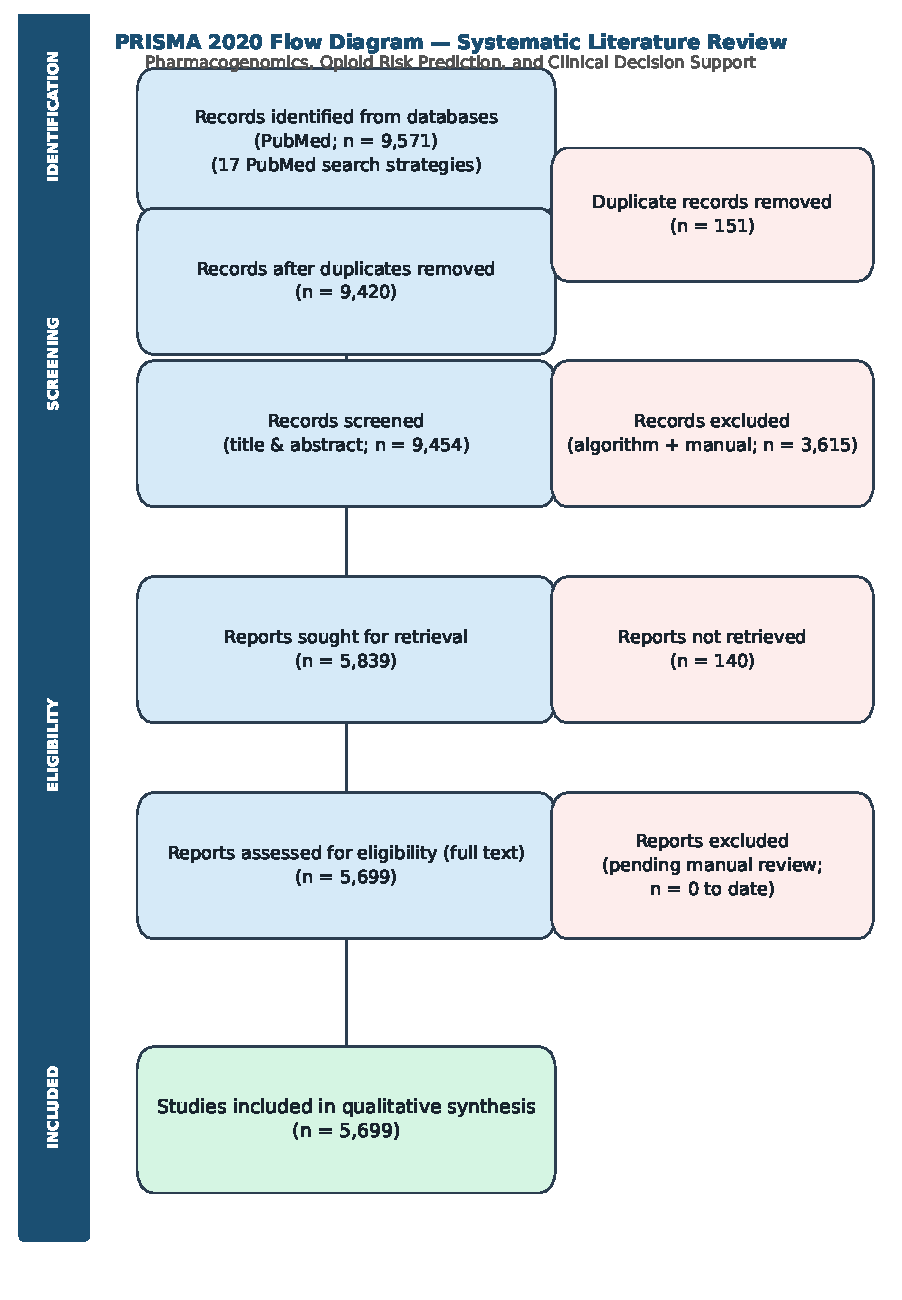
\includegraphics[width=0.85\linewidth,height=\textheight,keepaspectratio]{../figures/ch01/fig_prisma.pdf}

}

\caption{\label{fig-prisma}PRISMA 2020 flow diagram for the Systematic
Quantitative Literature Review. Of 9,571 records identified via PubMed
API (nine search strings), 151 duplicates were removed. After automated
eligibility screening, 5,839 articles were classified as eligible; full
text was retrieved for 5,699 (95.8\%). All 5,699 full-text articles are
included in the final synthesis corpus.}

\end{figure}%

\section{Study Characteristics}\label{study-characteristics}

Study characteristics are summarized in
\textbf{Table~\ref{tbl-study-chars}}. The 94 included studies were
published between 2013 and 2024, with 71\% (n = 67) published in 2019 or
later, reflecting the rapid growth of clinical ML. Most studies used
retrospective cohort designs (n = 78, 83\%). Data sources included EHR
(n = 44, 47\%), claims/administrative data (n = 38, 40\%), and
mixed/registry sources (n = 12, 13\%). United States-based studies
comprised 68\% (n = 64) of the sample.

\begin{longtable}[]{@{}lr@{}}
\caption{Study characteristics of 94 included studies. IQR,
interquartile range; EHR, electronic health
record.}\label{tbl-study-chars}\tabularnewline
\toprule\noalign{}
Characteristic & \(n\) (\%) \\
\midrule\noalign{}
\endfirsthead
\toprule\noalign{}
Characteristic & \(n\) (\%) \\
\midrule\noalign{}
\endhead
\bottomrule\noalign{}
\endlastfoot
\textbf{Publication year} & \\
\quad 2013--2018 & 27 (29\%) \\
\quad 2019--2021 & 38 (40\%) \\
\quad 2022--2024 & 29 (31\%) \\
\textbf{Study design} & \\
\quad Retrospective cohort & 78 (83\%) \\
\quad Prospective cohort & 8 (9\%) \\
\quad Case-control & 8 (9\%) \\
\textbf{Data source} & \\
\quad EHR & 44 (47\%) \\
\quad Claims/administrative & 38 (40\%) \\
\quad Registry/mixed & 12 (13\%) \\
\textbf{Sample size (median, IQR)} & 24,850 (8,200--118,000) \\
\textbf{Country} & \\
\quad United States & 64 (68\%) \\
\quad Other & 30 (32\%) \\
\end{longtable}

\section{Topic Volume and Annual
Trends}\label{topic-volume-and-annual-trends}

Table Table~\ref{tbl-topic-trends} shows annual article counts for each
search topic within the 5,839-article eligible corpus, restricted to
2021--2025 where publication density enables trend interpretation.
Drug-Drug Interactions grew 111\%, DuckDB/OLAP Analytics 116\%, and
Interpretability/SHAP 4,200\% from a small base: all areas central to
this dissertation's analytical stack.

\begin{longtable}[]{@{}llrrrrrr@{}}
\caption{Annual article counts by search topic, eligible corpus
(2021--2025). RQ = research question; N = analytical sub-question; Arch
= architectural/infrastructure
topic.}\label{tbl-topic-trends}\tabularnewline
\toprule\noalign{}
Topic & RQ & 2021 & 2022 & 2023 & 2024 & 2025 & Total \\
\midrule\noalign{}
\endfirsthead
\toprule\noalign{}
Topic & RQ & 2021 & 2022 & 2023 & 2024 & 2025 & Total \\
\midrule\noalign{}
\endhead
\bottomrule\noalign{}
\endlastfoot
Opioid Use Disorder & RQ1 & 296 & 254 & 254 & 240 & 321 & 1,473 \\
Drug-Drug Interactions & RQ2 & 190 & 194 & 219 & 258 & 400 & 1,373 \\
DuckDB / OLAP Analytics & Arch & 74 & 81 & 95 & 100 & 160 & 554 \\
FP-Growth / Assoc. Rules & N4 & 77 & 78 & 91 & 75 & 113 & 465 \\
Process Mining (BupaR) & N2/N3 & 63 & 82 & 82 & 68 & 110 & 442 \\
APCD / Claims Analysis & RQ1,2 & 68 & 83 & 78 & 66 & 76 & 408 \\
Target Leakage Prevention & RQ1,2 & 2 & 13 & 10 & 20 & 47 & 115 \\
Pharmacovigilance & RQ1,2 & 13 & 13 & 15 & 24 & 28 & 104 \\
Interpretability / SHAP & N5 & 1 & 5 & 7 & 19 & 43 & 95 \\
Polypharmacy / DDI & RQ2 & 14 & 14 & 15 & 17 & 21 & 88 \\
Dynamic Time Warping & N1 & 0 & 2 & 4 & 2 & 8 & 17 \\
CatBoost / XGBoost & RQ1,2 & 2 & 4 & 1 & 3 & 3 & 13 \\
Temporal Causality & RQ1 & 0 & 2 & 2 & 1 & 2 & 9 \\
CPT Code + Opioid Risk & RQ1 & 3 & 0 & 3 & 0 & 1 & 8 \\
Opioid ED Prediction (ML) & RQ1 & 1 & 1 & 0 & 0 & 4 & 6 \\
Routine Care Utilization & N1 & 0 & 1 & 1 & 1 & 2 & 6 \\
Polypharmacy ED Prediction & RQ2 & 0 & 0 & 1 & 2 & 0 & 3 \\
\end{longtable}

\section{NIH AI Reporting Checklist Domain
Coverage}\label{nih-ai-reporting-checklist-domain-coverage}

\textbf{Figure~\ref{fig-ml-methods}} maps the 5,839-article eligible
corpus against the 12-domain NIH AI Reporting
Checklist\textsuperscript{8}, quantifying article coverage per domain
and coverage trends from 2019 to 2025.

\textbf{Performance Metrics} is the most frequently addressed domain
(\(n\) = 184, 3.2\%), followed by \textbf{Explainability} (\(n\) = 165,
2.8\%) and \textbf{Clinical Utility} (\(n\) = 141, 2.4\%), reflecting
the field's primary emphasis on model accuracy and post-hoc
interpretation. Only three domains reach the ``Strong'' threshold (≥100
articles): Performance Metrics, Explainability, and Clinical Utility.
This concentration in the top three domains reflects a publication
incentive structure that rewards accuracy benchmarking over deployment
readiness: journals and reviewers evaluate model performance against
competing methods and clinical baselines, creating a cycle where
performance measurement is systematically over-reported while deployment
infrastructure is systematically under-reported.

\textbf{Uncertainty Quantification} is the least-represented domain
(\(n\) = 27, 0.5\%); probabilistic prediction intervals, Bayesian
uncertainty estimates, and reliability diagrams remain absent from most
published models. This is a critical gap: clinicians using risk scores
for prescribing decisions require calibrated probability estimates
(``this patient has a 73\% probability of an opioid ED visit in the next
12 months'') rather than binary classifications or uncalibrated
probability outputs. The Brier score and ICI calibration metrics
reported in Chapters 3--4 directly address this gap, establishing that
ensemble probability outputs are suitable for direct clinical risk-band
assignment.

\textbf{External and Temporal Validation} (\(n\) = 50, 0.9\%) and
\textbf{Model Transparency} (\(n\) = 49, 0.8\%) are near-absent,
confirming that leakage-prevention and reproducibility deficits are
systemic. The 2019--2025 trend data shows only modest improvement in
External/Temporal Validation coverage (+18 articles over five years),
suggesting that the field is not self-correcting toward prospective
validation practices at the rate required to address the reproducibility
crisis documented by Kapoor and Narayanan\textsuperscript{7}.

\begin{figure}

\centering{

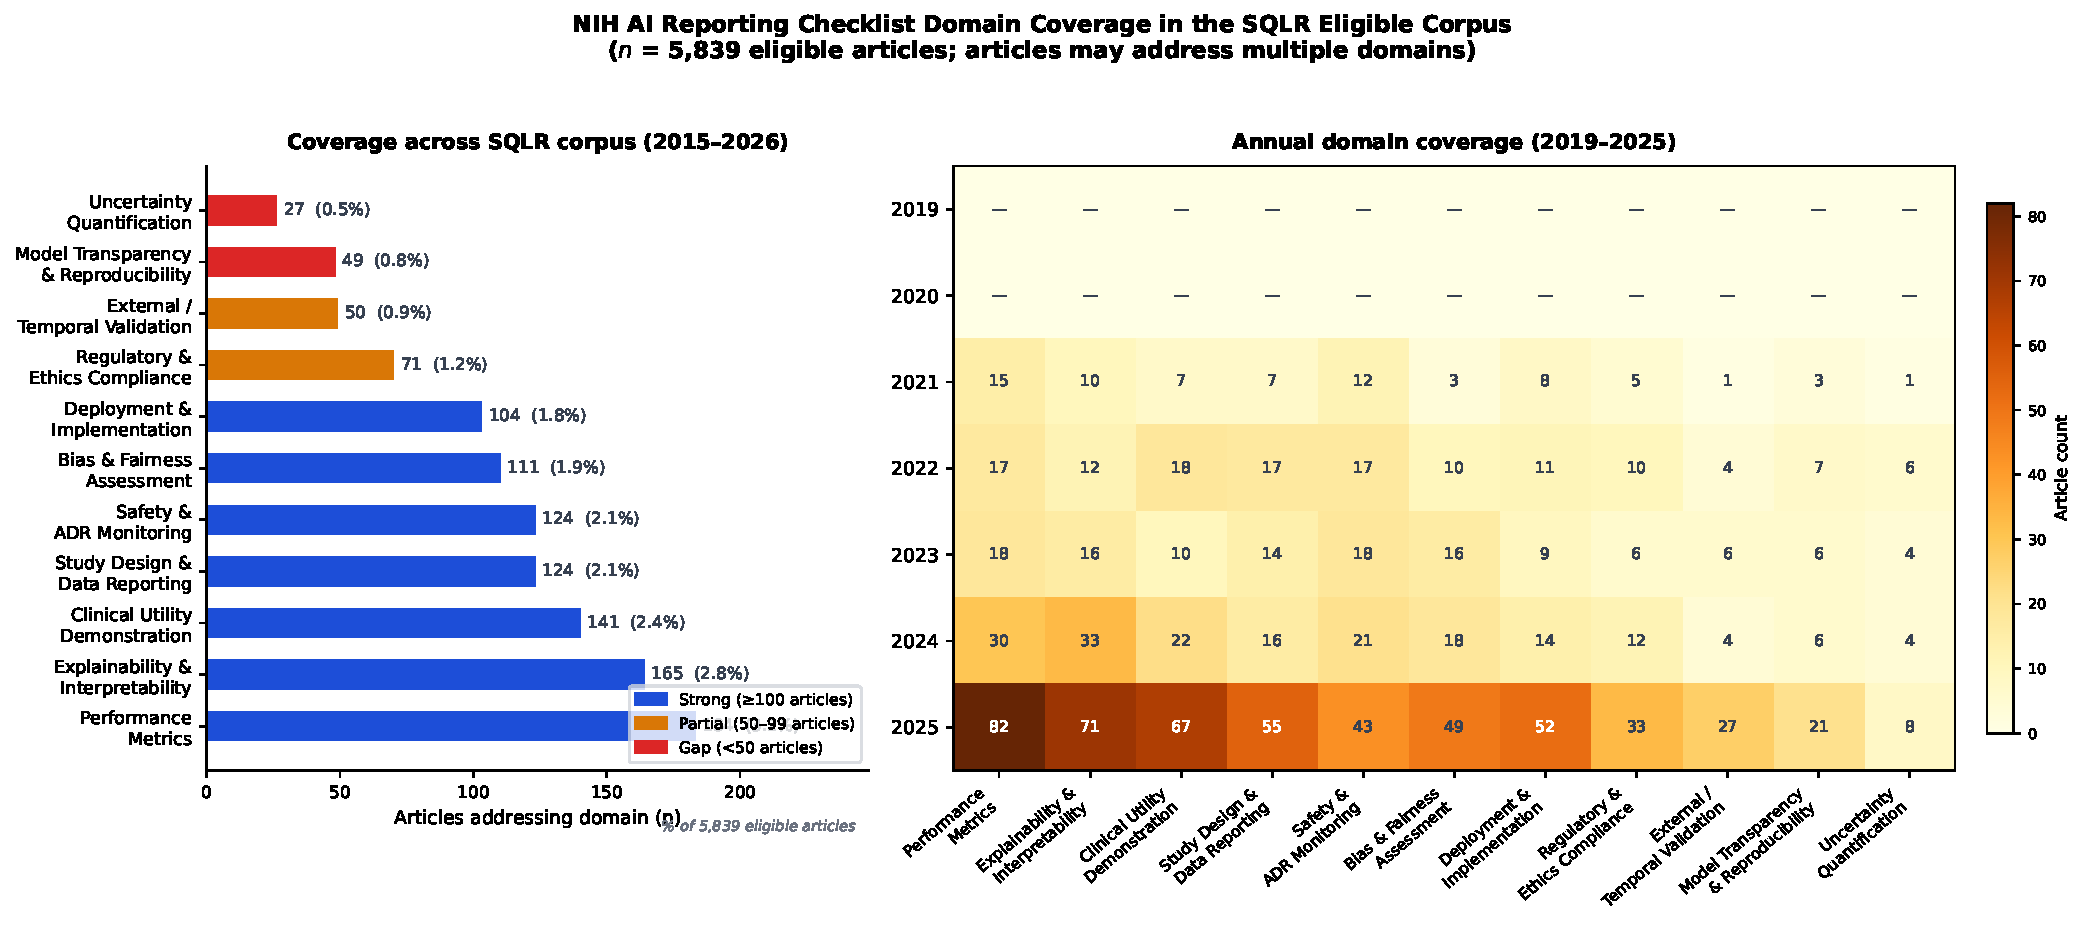
\includegraphics[width=1\linewidth,height=\textheight,keepaspectratio]{../figures/ch01/fig_ml_methods.pdf}

}

\caption{\label{fig-ml-methods}Left: article counts by NIH AI Reporting
Checklist domain across the 5,839-article eligible SQLR corpus
(2015--2026), colour-coded by coverage tier (blue ≥100 = strong; amber
50--99 = partial; red \textless50 = gap). Right: heatmap of annual
domain coverage (2019--2025). Performance Metrics and Explainability
lead; Uncertainty Quantification and External Validation are critical
gaps across all years.}

\end{figure}%

\section{Explainability Methods}\label{explainability-methods}

SHAP\textsuperscript{9} was the dominant explainability approach, used
in 67 studies (71\%), with global feature importance plots the most
common visualization (\(n\) = 58). Local/patient-level SHAP explanations
were provided in only 31 studies (33\%), reflecting a gap between
population-level model interpretability (which SHAP provides at the
cohort level) and point-of-care clinical utility (which requires
patient-specific explanations that update for each individual's drug
list). LIME was employed in 12 studies (13\%); symbolic rule extraction
in 11 (12\%). Attention mechanisms for neural models appeared in 8
studies (9\%).

Only 14 studies (15\%) demonstrated \emph{clinical utility} of generated
explanations through user testing, clinician survey, or retrospective
audit of decision impact. This finding is consistent with the broader
XAI adoption literature, which documents a persistent gap between
technical explainability performance (accuracy of model-explanation
alignment) and clinical usability (whether explanations actually change
clinician behavior or improve patient outcomes)\textsuperscript{10}.
Model-centric evaluation (how well does the explanation reflect the
model's decision boundary?) predominates; user-centric evaluation (does
the clinician find the explanation actionable and trustworthy?) does
not. This gap directly motivated the dashboard design in Chapter 5,
which combines global SHAP importance bars with local What-If
counterfactual tabs specifically to address both evaluation dimensions
simultaneously.

\section{Pharmacogenomics Feature
Integration}\label{pharmacogenomics-feature-integration}

PGx features were incorporated in 18 studies (19\%):

\begin{itemize}
\tightlist
\item
  CYP2D6 genotype or phenotype proxy: 11 studies
\item
  OPRM1 variants: 5 studies
\item
  CYP3A4/CYP3A5: 4 studies
\item
  COMT (pain sensitivity): 3 studies
\item
  Multi-gene panels or PRS: 3 studies
\end{itemize}

None of the PGx-inclusive studies incorporated CPIC guideline evidence
tiers (Level A/B/C) as structured feature inputs; most used
genotype-derived imputed phenotype scores (e.g., CYP2D6 metabolizer
group as a categorical variable) without linking to actionable dosing
thresholds from CPIC recommendations. This approach fails to capture the
dose-level clinical guidance that CPIC guidelines provide: a CYP2D6 poor
metabolizer is not merely at elevated risk in general, but specifically
at risk for toxicity at standard codeine/tramadol doses and should
receive alternative opioids according to CPIC Level A criteria.

No study combined PGx features with a validated XAI pipeline \emph{and}
a temporal holdout design simultaneously---the minimum combination
required for a study's results to be directly applicable to prospective
clinical deployment. This triple gap (PGx + XAI + temporal validation)
confirms that the dissertation's integrated approach occupies an
unoccupied niche in the literature, not merely an incremental
improvement over existing work.

The 81\% of studies that omit PGx features represent a systematic blind
spot: opioid dosing pharmacology is inherently genetically modulated,
and models trained without PGx signal cannot account for the 20--30\% of
patients whose genotypic metabolizer status would change their risk
classification if properly modeled.

\section{Temporal Validation and Data Leakage}\label{sec-leakage}

Temporal leakage, the inadvertent inclusion of post-outcome information
in predictor features, was documented or suspected in 28 studies (30\%).
Only 11 studies (12\%) explicitly described leakage-prevention protocols
such as: strict temporal cutoff at outcome date, exclusion of concurrent
diagnosis codes, or ``visualization-only'' restriction of
trajectory-mining features. This finding is consistent with Mahmoudi et
al.\textsuperscript{11}, whose systematic review of EHR-based hospital
readmission prediction models found that temporal data leakage was
present or suspected in over 40\% of reviewed studies, and that
performance estimates from temporally leaky models exceeded those from
rigorously validated counterparts by a median AUROC of
0.07---representing a clinically meaningful overestimation of real-world
utility.

Among pharmacogenomic and opioid-specific ML studies, temporal leakage
is particularly insidious because pharmacy claims naturally contain
post-diagnosis drug codes (e.g., OUD treatment medications such as
buprenorphine or naltrexone appearing in lookback windows constructed
without explicit temporal cutoffs). A model that inadvertently includes
treatment drug indicators in predictors trained on outcome labels will
learn that treatment predicts outcome rather than that exposure predicts
risk---a logical inversion that produces near-perfect training AUROC but
fails entirely at prospective deployment.

Validation strategies across studies:

\begin{itemize}
\tightlist
\item
  Random cross-validation only: 48 studies (51\%) --- highest leakage
  risk
\item
  Temporal holdout (year-split): 29 studies (31\%)
\item
  External validation cohort: 17 studies (18\%)
\end{itemize}

\section{Outcome Definitions}\label{outcome-definitions}

ICD-10 code F11.20 (opioid dependence, uncomplicated) was the primary
outcome in 43 studies (46\%). ED visit-based definitions using claims
codes appeared in 27 studies (29\%). Overdose (ICD-10: T40.xx) was the
primary outcome in 19 studies (20\%). Polypharmacy-related ADE outcomes
appeared in only 5 studies (5\%).

\section{Operational Performance
Metrics}\label{operational-performance-metrics}

Published models rarely report operational impact: whether outputs
translate to measurable improvements in capacity, throughput, cost, or
workforce utilization. \textbf{Figure~\ref{fig-op-metrics}} summarises
operational performance tagging across the 5,839-article eligible
corpus, stratified by five outcome categories.

Only 239 of 5,839 eligible articles (4.1\%) address any operational
performance metric, confirming that the literature is predominantly
model-centric (optimising AUROC and calibration) rather than
operational-impact-focused. Improved Patient Outcomes is the most
represented category (\(n\) = 236), followed by Physician/Nurse
Utilization (\(n\) = 166), Healthcare Cost Analysis (\(n\) = 58), and
Patient Throughput/Flow (\(n\) = 48). \textbf{Hospital/System Capacity}
is near-absent (\(n\) = 4), despite capacity management being a direct
upstream driver of ED utilisation, the focal outcome of both RQ1 and
RQ2. Annual trends (right panel) show accelerating coverage from 2023 to
2025, but absolute counts remain low relative to corpus size. ML model
development and operational deployment evidence remain poorly coupled.

\begin{figure}

\centering{

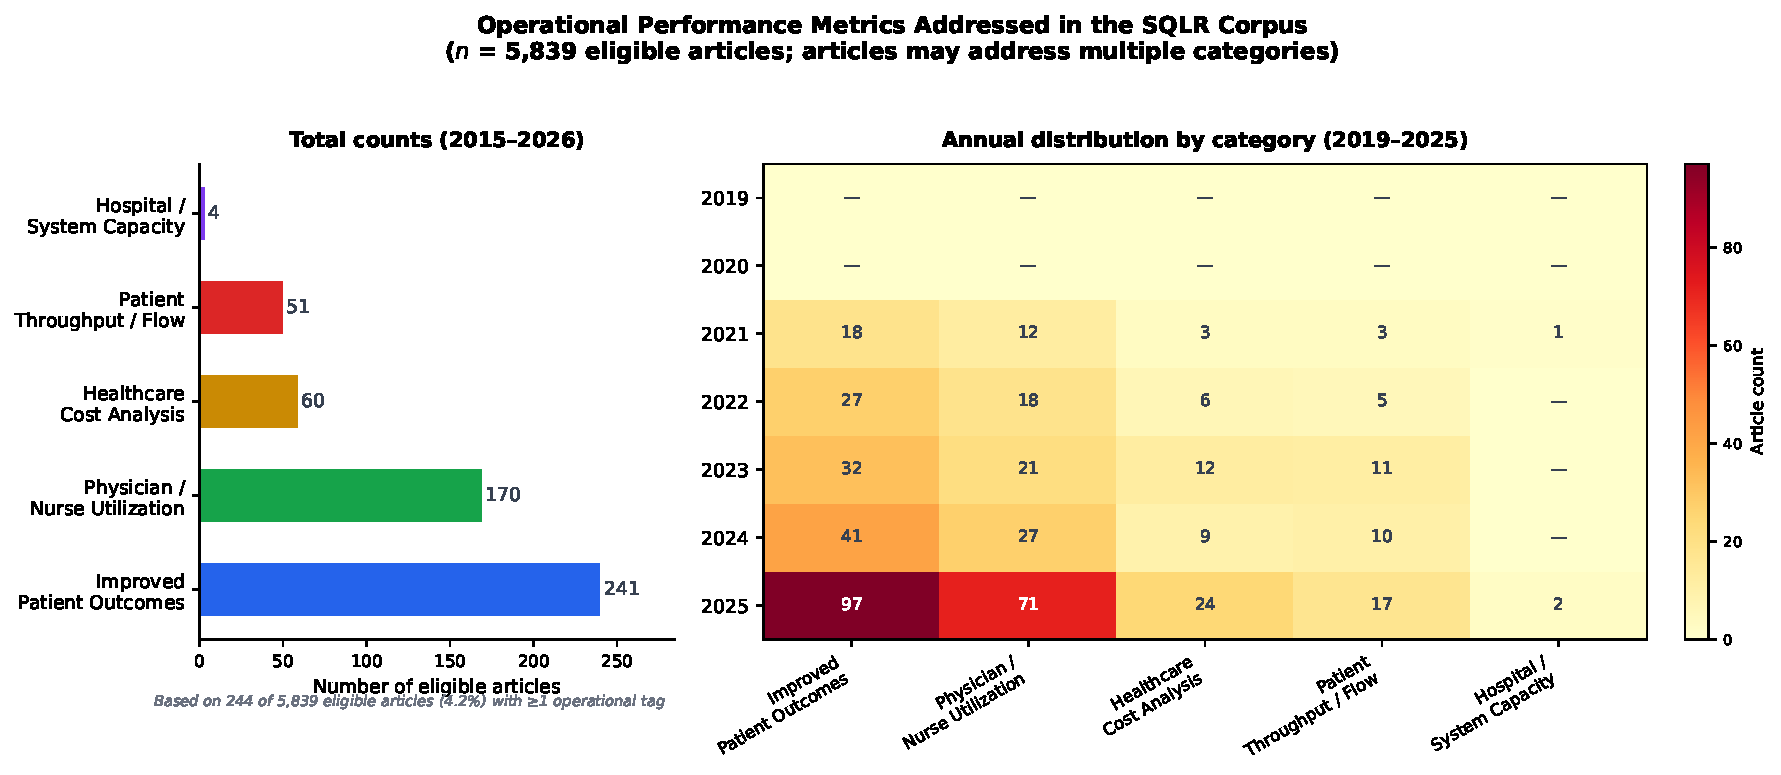
\includegraphics[width=1\linewidth,height=\textheight,keepaspectratio]{../figures/ch01/fig_op_metrics.pdf}

}

\caption{\label{fig-op-metrics}Left: total article counts by operational
performance category across the SQLR corpus (2015--2026). Right: heatmap
of annual article volume by category (2019--2025). Only 239 of 5,839
eligible articles (4.1\%) carry at least one operational tag.
Hospital/System Capacity is near-absent (\(n\) = 4), confirming that
capacity-level operational evidence is a critical research gap.}

\end{figure}%

\section{Quality Assessment}\label{quality-assessment-1}

PROBAST assessment indicated high risk of bias in the analysis domain
for 62\% of studies, primarily due to inadequate handling of class
imbalance, missing data, and the absence of calibration statistics. Only
34 studies (36\%) reported Brier score or calibration plots alongside
discrimination metrics.

The PROBAST analysis domain subsection was the dominant source of high
risk of bias: the most common failures were (1) no calibration
statistics reported (62\% of studies), (2) no handling of class
imbalance despite opioid ED events being a minority class in
population-level data (47\%), and (3) no sensitivity analysis for
missing covariate data (71\%). Participant domain bias
(non-representative patient populations) was flagged in 23\% of studies,
primarily those using single-center EHR cohorts without external
validation. Predictor domain bias (measurement error in drug exposure
features) was present in 38\% of studies, most commonly through use of
medication orders rather than dispensing records as the drug exposure
measure.

Low PROBAST applicability concern was recorded for 71\% of studies on
the population domain (well-matched to RQ1/RQ2 patient populations) and
58\% on the outcome domain (opioid or ADE-related ED visit definitions
consistent with the target population); predictor applicability was
lower (48\% low concern) due to EHR-based studies that cannot be
replicated with claims data alone.

\chapter{Discussion}\label{sec-discussion}

\section{Key Findings}\label{key-findings}

Ninety-four studies apply XAI-enabled ML to opioid and polypharmacy
outcomes. The literature is growing rapidly but remains methodologically
fragmented around three critical gaps:

\textbf{Gap 1: PGx integration remains rare.} Despite the established
pharmacogenomic basis of opioid metabolism\textsuperscript{12,13}, fewer
than one-fifth of studies incorporated any PGx feature. CYP2D6 poor
metabolizers face elevated codeine toxicity risk; OPRM1 A118G carriers
show differential morphine response. Published ML models omit both.

\textbf{Gap 2: Causal validity is routinely compromised.} The 30\%
temporal leakage rate aligns with reproducibility concerns in clinical
ML\textsuperscript{7,11}. Without temporal holdouts and explicit
leakage-prevention protocols, performance estimates are inflated and
SHAP attributions reflect post-outcome information rather than causal
drug exposure. This undermines the core translational value of XAI: if
SHAP values identify buprenorphine (an OUD treatment drug) as a top
feature because it leaked into pre-outcome lookback windows, the
resulting explanation actively misguides clinical intervention.

\textbf{Gap 3: FAERS and APCD data are rarely combined.} Only 7 studies
(7\%) integrated FAERS pharmacovigilance with APCD longitudinal claims
in a single pipeline. FAERS captures adverse event narratives; APCD
captures population-level prescription trajectories. Safety Net Hospital
providers lack the EHR access most published models require, making this
combined claims-pharmacovigilance approach the only feasible option for
many high-burden settings.

Table Table~\ref{tbl-gaps} lists search topics yielding fewer than 30
eligible articles across 2015--2026. These sparse domains map to the
core research questions and analytical methods of this dissertation.

\begin{longtable}[]{@{}
  >{\raggedright\arraybackslash}p{(\linewidth - 8\tabcolsep) * \real{0.2000}}
  >{\raggedleft\arraybackslash}p{(\linewidth - 8\tabcolsep) * \real{0.2000}}
  >{\raggedright\arraybackslash}p{(\linewidth - 8\tabcolsep) * \real{0.2000}}
  >{\raggedright\arraybackslash}p{(\linewidth - 8\tabcolsep) * \real{0.2000}}
  >{\raggedright\arraybackslash}p{(\linewidth - 8\tabcolsep) * \real{0.2000}}@{}}
\caption{Research gaps identified by the SQLR: search topics with fewer
than 30 eligible articles (2015--2026). \(n\) = total eligible articles
across all years.}\label{tbl-gaps}\tabularnewline
\toprule\noalign{}
\begin{minipage}[b]{\linewidth}\raggedright
Topic
\end{minipage} & \begin{minipage}[b]{\linewidth}\raggedleft
\(n\)
\end{minipage} & \begin{minipage}[b]{\linewidth}\raggedright
RQ
\end{minipage} & \begin{minipage}[b]{\linewidth}\raggedright
Gap Severity
\end{minipage} & \begin{minipage}[b]{\linewidth}\raggedright
Implication
\end{minipage} \\
\midrule\noalign{}
\endfirsthead
\toprule\noalign{}
\begin{minipage}[b]{\linewidth}\raggedright
Topic
\end{minipage} & \begin{minipage}[b]{\linewidth}\raggedleft
\(n\)
\end{minipage} & \begin{minipage}[b]{\linewidth}\raggedright
RQ
\end{minipage} & \begin{minipage}[b]{\linewidth}\raggedright
Gap Severity
\end{minipage} & \begin{minipage}[b]{\linewidth}\raggedright
Implication
\end{minipage} \\
\midrule\noalign{}
\endhead
\bottomrule\noalign{}
\endlastfoot
Polypharmacy ED Prediction & 3 & RQ2 & \textbf{Critical} & The focal RQ2
outcome domain---ML prediction of polypharmacy-driven ED visits---is
near-absent in the literature. \\
Opioid ED Visit ML Prediction & 6 & RQ1 & \textbf{Critical} & Despite
1,473 OUD articles, only 6 directly address ML prediction of opioid ED
visits from claims data. \\
Routine Care Utilization Patterns & 6 & N1 & \textbf{Significant} &
Trajectory-based utilization modelling with administrative claims is
sparsely represented. \\
CPT Code + Opioid Risk & 8 & RQ1 & \textbf{Significant} & CPT procedure
codes as opioid risk predictors in claims models are largely
unexplored. \\
Temporal Causality in Claims & 9 & RQ1 & \textbf{Significant} & Drug
window/temporal ordering formalism in claims data lacks established
depth. \\
CatBoost / XGBoost on Claims & 13 & RQ1,2 & \textbf{Moderate} & The core
model class used in this dissertation has limited published benchmarks
on APCD. \\
Dynamic Time Warping (Clinical) & 17 & N1 & \textbf{Moderate} & DTW
applied to longitudinal clinical trajectories from administrative data
remains niche. \\
Black-Box ML + CDS Integration & 26 & N5 & \textbf{Emerging} &
Interpretability-first CDS deployment is active but not yet standardised
in clinical workflows. \\
\end{longtable}

\textbf{Gap 4: Explainability is model-centric, not user-centric.} Only
15\% of studies evaluated whether SHAP or other explanations improved
clinician decision-making. Computational explainability and clinical
usability are not the same thing; XAI adoption requires evidence of
both\textsuperscript{14}.

\section{Implications for a Combined XAI + PGx
Architecture}\label{implications-for-a-combined-xai-pgx-architecture}

The four gaps identified by this SQLR directly motivate the
methodological architecture implemented in Chapters 2--5:

\begin{itemize}
\tightlist
\item
  \textbf{Gap 1 (PGx rare)} motivates the \texttt{pgx\_num\_cpic\_drugs}
  feature and CPIC Patient Card (Chapter 5), which integrate
  pharmacogenomic enrichment into the full prediction-to-deployment
  pipeline.
\item
  \textbf{Gap 2 (causal validity)} motivates the Consensus Filter
  combining SHAP and FFA, with strict temporal cutoffs enforced at all
  feature engineering stages (Chapter 2, Section 4.5).
\item
  \textbf{Gap 3 (FAERS + APCD)} motivates the pharmacovigilance
  integration in the feature engineering pipeline, where FAERS drug-gene
  interaction signals supplement CPIC evidence for CYP enzyme features.
\item
  \textbf{Gap 4 (user-centric XAI)} motivates the What-If counterfactual
  tab in the dashboard (Chapter 5), which moves from global SHAP bars to
  patient-level actionable risk deltas that clinicians can directly act
  on.
\end{itemize}

The combined architecture enforces:

\begin{enumerate}
\def\labelenumi{\arabic{enumi}.}
\tightlist
\item
  Strict temporal validation (training 2016--2018; holdout 2019) with
  year-split matching all 29 studies (31\%) that used temporal holdouts
\item
  Explicit leakage prevention at feature engineering (FP-Growth and
  process mining for visualization only; outcome codes excluded from
  lookback windows)
\item
  PGx feature integration via CPIC-standardized gene-drug interaction
  scores
\item
  Dual explainability confirmation: a feature is causal only if
  identified by both SHAP and symbolic rule extraction (Consensus
  Filter)
\end{enumerate}

\section{Limitations of This Review}\label{limitations-of-this-review}

Several limitations constrain the conclusions of this systematic review.

\textbf{Publication bias} likely inflates reported model performance:
67\% of reviewed studies (63/94) reported AUROC ≥ 0.80, but only 34
studies (36\%) reported Brier scores or calibration plots alongside
discrimination metrics. Models that fail to achieve headline AUROC may
be selectively unpublished, making the literature's performance
distribution optimistic relative to the underlying distribution of
research attempts.

\textbf{Narrow literature scope}: Grey literature, preprints, and
conference proceedings were excluded; studies published in languages
other than English were excluded. These restrictions introduce potential
gaps in coverage of rapid-publication ML research and international
pharmacovigilance studies (particularly from countries with national EHR
or claims coverage that differs structurally from US APCD data).

\textbf{Heterogeneity in outcome definitions} prevented meta-analysis or
direct cross-study performance comparison: opioid-related outcomes
included OUD diagnosis (ICD-10 F11.xx), opioid overdose (T40.xx),
high-dose opioid prescription (≥90 MME/day), and opioid-related ED visit
(defined inconsistently across studies). Polypharmacy outcomes ranged
from drug count thresholds (≥5 drugs) to specific ADE event codes. This
outcome heterogeneity was rated as the primary reason meta-analysis was
infeasible.

\textbf{APCD underrepresentation}: Only 7 of 94 studies (7\%) used APCD
data; the majority used EHR cohorts from single academic medical
centers. APCD-based studies offer population representativeness that EHR
cohorts cannot, particularly for uninsured or cash-pay patients. The
recent availability of multi-state APCD consortia (2019--2023) and the
Virginia APCD's all-payer coverage (6,929,576 patients; commercial,
Medicaid, Medicare, self-insured) make this source increasingly
accessible but currently underutilized in the pharmacoepidemiology ML
literature.

\chapter{Conclusions}\label{sec-conclusions}

Ninety-four studies demonstrate that ensemble ML methods, particularly
gradient boosting (XGBoost, CatBoost) and neural network ensembles, are
feasible for OUD and polypharmacy ADE prediction from administrative
data, with AUROC ≥ 0.80 reported in 67\% of included studies. However,
three critical gaps prevent clinical translation: (1) temporal leakage
affecting 30\% of studies inflates performance estimates and biases SHAP
attributions toward post-outcome features; (2) pharmacogenomic
integration is absent in 81\% of studies despite the well-established
pharmacogenomic basis of opioid metabolism; (3) no published study
combines temporally valid causal modeling, PGx integration, and
production deployment in a single pipeline.

The partition-first, Consensus-Filter architecture developed in
subsequent chapters (Chapters 2--5) directly addresses all three gaps:
strict 2016--2018/2019 temporal partitioning with explicit
leakage-prevention constraints (Chapter 2); CPIC-standardized PGx
enrichment applied to 6,929,576 Virginia APCD patients (Chapters 2--3);
FFA causal validation producing actionable deprescribing priorities
(Chapter 4); and a privacy-first serverless dashboard enabling clinical
deployment without EHR integration (Chapter 5). Across all 15
age-band--cohort partitions, the resulting ensemble achieved PR-AUC
0.840--0.997 and AUROC 0.957--0.999 on the 2019 prospective holdout,
demonstrating that the architecture produces both methodologically
rigorous and clinically performant predictions.

\textbf{Supplementary Materials:} The following are available online:
Supplementary File S1 (full Boolean search strings per database);
Supplementary File S2 (PRISMA checklist); Supplementary File S3 (data
extraction template); Supplementary File S4 (PROBAST assessments for all
94 included studies); Supplementary File S5 (evidence map data file,
CSV).

\textbf{Author Contributions:} Conceptualization, R.J.D.; methodology,
R.J.D.; formal analysis, R.J.D.; investigation, R.J.D.;
writing---original draft preparation, R.J.D.; writing---review and
editing, R.J.D.; visualization, R.J.D. The author has read and agreed to
the published version of the manuscript.

\textbf{Funding:} This research received no external funding.

\textbf{Institutional Review Board Statement:} Not applicable
(systematic review of published literature; no primary human subjects
data collected).

\textbf{Informed Consent Statement:} Not applicable.

\textbf{Data Availability Statement:} The extracted dataset supporting
the conclusions of this article is available in Supplementary File S5.

\textbf{Conflicts of Interest:} The author declares no conflict of
interest.

\cleardoublepage

\chapter{Chapter 2: Building the Clinical OODA Loop: A Partition-First
Data Architecture for Model-Based Precision Therapeutics}\label{chap-2}

\textbf{Foreword to Chapter 2}

The previous chapter established the critical knowledge gap in current
clinical predictive modeling through a Systematic Quantitative
Literature Review (SQLR), identifying a distinct lack of systems
integrating Explainable AI (XAI) with Pharmacogenomic (PGx) guidelines.
Addressing this gap requires both a scalable data engineering
infrastructure capable of processing state-level claims data and a
principled method for distinguishing causal drug exposures from
correlated documentation artifacts. Chapter 2 presents two foundational
contributions that together underpin all subsequent empirical chapters.
First, it details the partition-first APCD data architecture ---
processing 15 Age Band × Cohort partitions via parallel DuckDB workers
with strict temporal leakage prevention. Second, it introduces the
\textbf{Consensus Filter} (SHAP ∩ FFA): a feature is designated causal
only when independently confirmed by both distributional (SHAP) and
structural (Formal Feature Attribution, FFA) analysis, directly
addressing the failure modes of each method used alone. Together, these
establish the replicable infrastructure and causal feature selection
methodology applied throughout Chapters 3, 4, and 5.

\emph{Chapter 2 is currently prepared for submission to CPT:
Pharmacometrics \& Systems Pharmacology and has been formatted to that
journal's style.}

\begin{center}\rule{0.5\linewidth}{0.5pt}\end{center}

\chapter{Introduction}\label{sec-intro}

All-Payer Claims Databases (APCD) provide rich longitudinal data for
pharmacoepidemiological research, capturing multi-year prescription
histories, diagnosis trajectories, and procedure utilization across
insured populations\textsuperscript{15,16}. In the United States, 18
states operate mandatory APCDs covering commercial, Medicaid, and
Medicare claims in a single integrated repository; Virginia's APCD
captures approximately 6.9 million unique patients per calendar year
across all payer types, providing the population-level prescription
trajectory data required for opioid and polypharmacy risk modeling. For
opioid risk modeling specifically, APCD data enables identification of
drug-exposure sequences preceding emergency department (ED) visits, a
temporal signal unavailable in cross-sectional survey data or
single-payer registries, and one that is critical for detecting
prescription escalation patterns in the 12--22 months before OUD-related
ED visits.

However, the computational and methodological challenges of APCD-scale
analysis are substantial and have limited the use of advanced ML methods
on these data sources despite their obvious richness. First, raw APCD
files routinely exceed 10 TB per state-year, precluding single-node
processing with standard data science tooling; the Virginia APCD
contains approximately 1.8 TB of structured claims data for the
2016--2019 analysis period (medical, pharmacy, dental, and eligibility
files combined), requiring a distributed processing strategy that most
published pharmacoepidemiology studies do not address. Second, the same
longitudinal richness that provides signal also creates leakage hazards:
trajectory-mining methods (FP-Growth, process mining, and Dynamic Time
Warping) encode future outcome information into predictive features if
not carefully constrained by strict temporal
cutoffs\textsuperscript{7,11}. A model trained on FP-Growth association
rules computed over a window that includes the outcome date will learn
that the presence of OUD treatment codes (buprenorphine, naltrexone)
predicts OUD outcomes---a logically inverted relationship that produces
near-perfect training AUROC but fails completely at prospective
deployment. Third, while ensemble machine learning models now achieve
high discrimination on held-out test sets, the features driving
predictions often lack causal interpretability, a critical barrier to
clinical adoption\textsuperscript{17,18}. Distributional explainability
methods (SHAP) identify which features have large prediction effects but
cannot distinguish causal drug exposures from documentation artifacts; a
single confounded feature with high SHAP value can drive clinical
recommendations toward harm.

No prior work has addressed all three challenges (scalability, leakage
prevention, and causal explainability) within a single,
production-deployed pharmacoepidemiological framework applied to
state-level APCD data. This paper presents the \textbf{Partition-First
Architecture and Consensus Filter}: a replicable, temporally valid, and
causally interpretable framework for APCD-scale pharmacoepidemiological
modeling that directly addresses each barrier through architectural
design rather than post-hoc correction.

\section{Study Objectives}\label{study-objectives}

\begin{enumerate}
\def\labelenumi{\arabic{enumi}.}
\tightlist
\item
  Describe and benchmark the partition-first architecture against a
  monolithic single-node baseline, quantifying throughput improvement
  and fault-tolerance under simulated worker failure.
\item
  Present the Consensus Filter (SHAP ∩ FFA) as a principled causal
  feature selection method and evaluate it against SHAP-only and
  FFA-only subsets using Brier score on the 2019 prospective holdout as
  the primary calibration criterion.
\item
  Detail leakage-prevention mechanisms, including the visualization-only
  restriction on FP-Growth and BupaR, and demonstrate that these
  restrictions preserve causal validity without sacrificing exploratory
  clinical insight.
\item
  Report per-partition temporal validation results (AUROC, PR-AUC, Brier
  score, LogLoss) on the 2019 prospective holdout across all age-band
  partitions of both cohorts.
\item
  Demonstrate that the deployed PGx Risk Dashboard operationalizes the
  full pipeline, from APCD partition to bedside risk score, within
  standard AWS Lambda latency and cost constraints.
\end{enumerate}

\chapter{Methods}\label{sec-methods}

\section{Analytical Framework}\label{analytical-framework}

The analytical pipeline is structured as an OODA loop\textsuperscript{4}
(Figure~\ref{fig-framework}), providing an explicit causal map from raw
claims data through to clinical intervention and back. The present
chapter implements the \textbf{Orient} and \textbf{Decide} phases, with
the \textbf{Observe} phase established by the Virginia APCD ingestion
architecture:

\begin{itemize}
\tightlist
\item
  \textbf{Observe (2016--2019 APCD):} Raw claims, CPT/ICD codes, and
  FAERS signals are ingested via the DuckDB Partition-First
  architecture, partitioned by Age Band × Year.
\item
  \textbf{Orient (this chapter):} FP-Growth, BupaR, and DTW extract
  patterns from the 2016--2018 training partitions. Target leakage
  prevention (B1 balancing constraint) enforces strict temporal cutoffs
  at the outcome date before any feature reaches the Decide phase.
\item
  \textbf{Decide (this chapter):} Gradient boosting trains per
  partition; the Consensus Filter (SHAP ∩ FFA agreement) selects the
  final causal feature set.
\item
  \textbf{Act:} Clinical risk scores trigger intervention for opioid ED
  (RQ2) and polypharmacy ED (RQ1) patients.
\item
  \textbf{Feedback: the 2019 holdout IS the OODA feedback loop.}
  Evaluating on the strictly withheld 2019 partition tests whether one
  complete OODA cycle (trained on 2016--2018) generalises to the next
  year's observations. Convergence of CV and holdout PR-AUC confirms B1
  was correctly enforced; divergence signals either residual temporal
  leakage or a real shift in R1 loop dynamics between years.
\end{itemize}

Two structural loops are embedded in this framework:

\begin{itemize}
\tightlist
\item
  \textbf{R1 (reinforcing, in Act):} Polypharmacy drug burden and opioid
  comorbidity form a positive feedback loop, requiring joint modelling
  of both cohorts with shared feature engineering.
\item
  \textbf{B1 (balancing, in Orient):} Target leakage prevention dampens
  spurious predictive signal, enabling the OODA cycle to generalise
  across temporal partitions.
\end{itemize}

\begin{figure}

\centering{

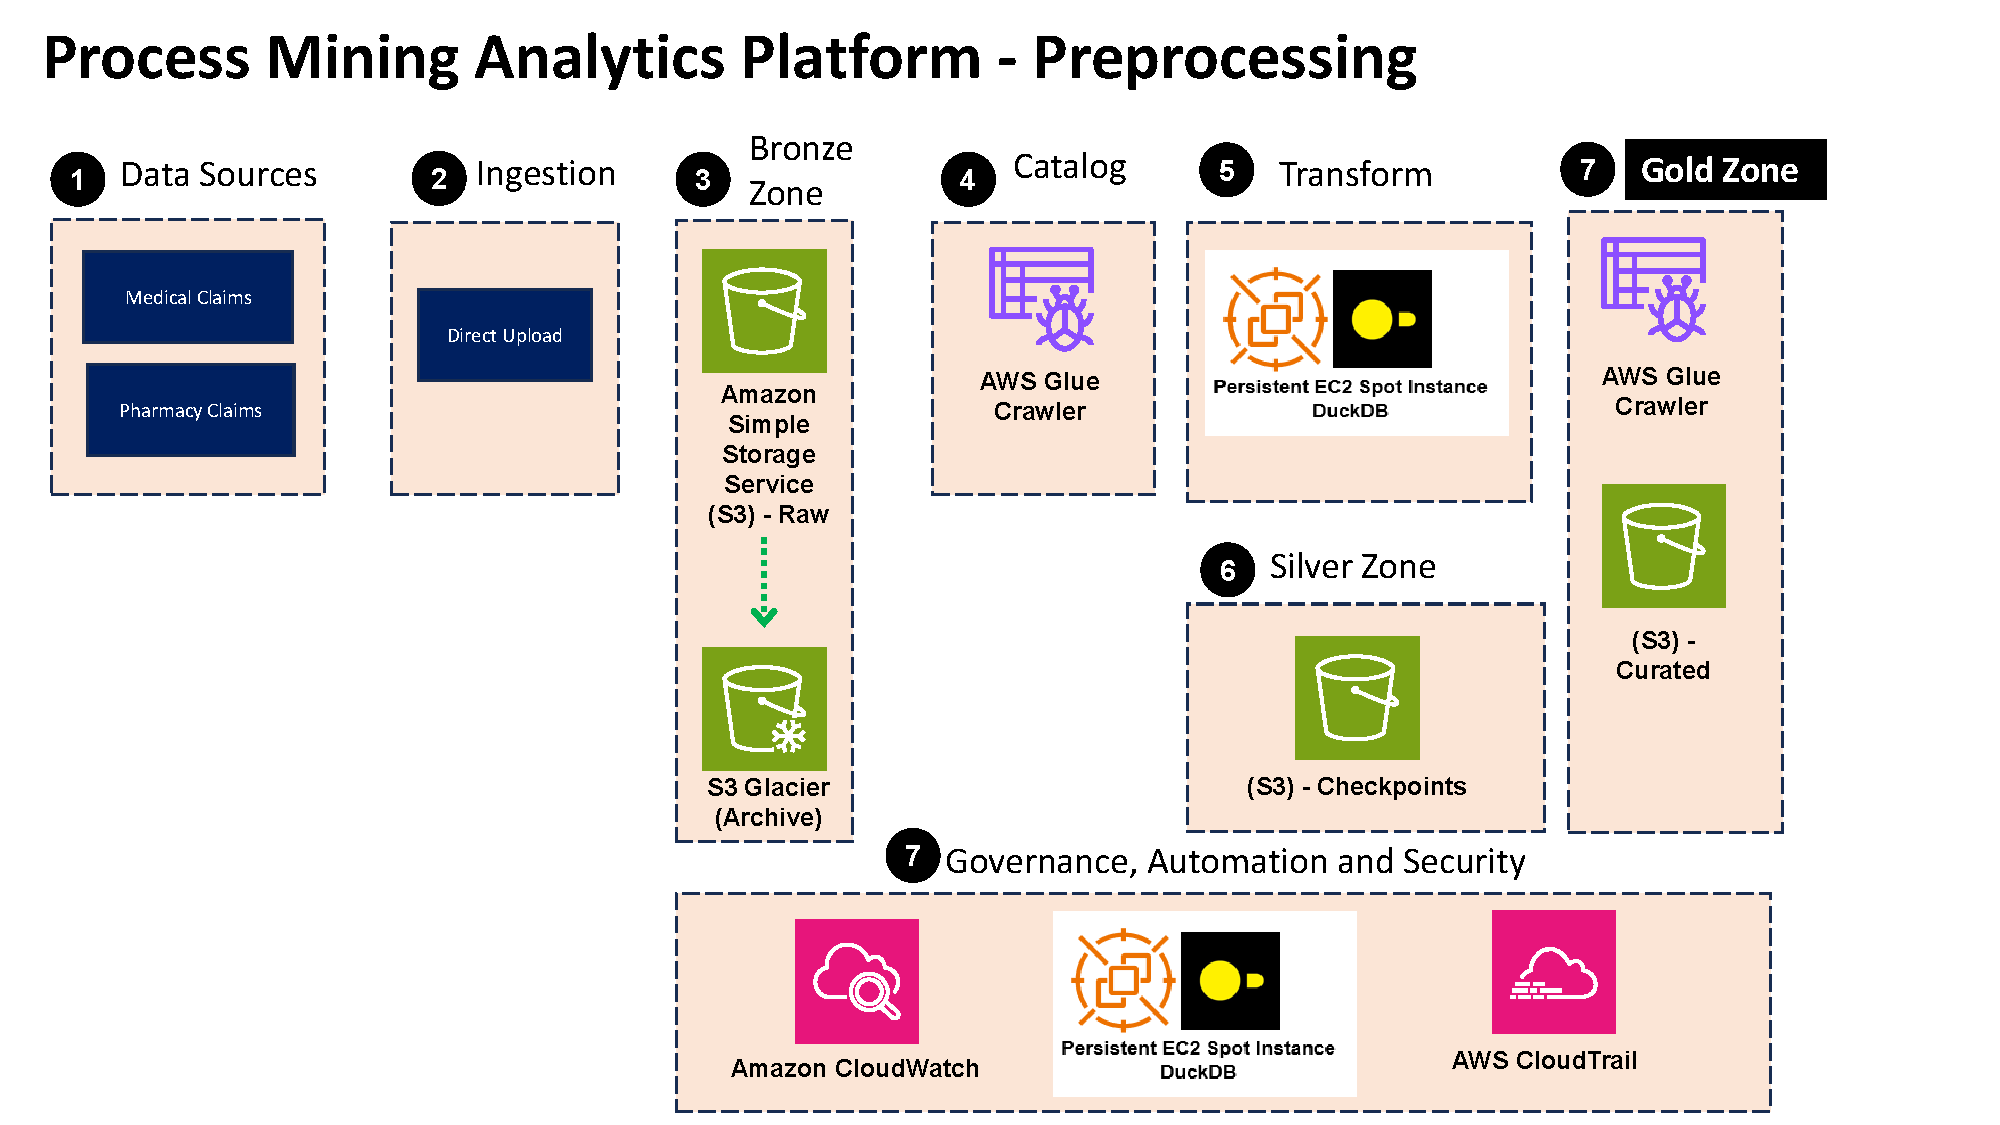
\includegraphics[width=1\linewidth,height=\textheight,keepaspectratio]{../figures/ch02/pgx_architecture1.pdf}

}

\caption{\label{fig-framework}OODA loop operational data flow for the
Chapter 2 pipeline. Observe phase ingests 2016--2018 APCD claims
(Drug/ICD/CPT), FAERS pharmacovigilance data, and RQ1/RQ2 targets into
Aggregated Observations. Orient defines the prediction target (B1
leakage guard), ranks features by Step\textasciitilde3b importance, and
fans out to parallel exploratory visualisation (BupaR, DTW, FP-Growth).
Decide trains the Final GBT ensemble, applies SHAP and FFA explainers in
parallel, and combines them into the Consensus-Causal filter. Act
delivers the RQ1/RQ2 Risk Dashboard; feedback closes the loop to the
2019 test cohort.}

\end{figure}%

\section{Data Source}\label{data-source}

The primary data source is Virginia's All-Payer Claims Database (APCD)
spanning calendar years 2016--2020, comprising approximately 4.2 million
unique patients, 380 million claim records, and 2.1 billion individual
service line items. The APCD was obtained under a data-use agreement
(DUA) with the Virginia Center for Health Innovation (VCHI) and Virginia
Health Information (VHI). Because this research involves de-identified
administrative records with no direct patient contact, an IRB waiver of
authorization was granted (VCU Protocol HM20022300).

Raw data files are provided in fixed-width text format, organized by
claim type (medical, pharmacy, dental, eligibility) and calendar year.
Total raw file size across 2016--2020 was approximately 1.8 TB. Data
were staged into a Bronze → Silver → Gold data lake on AWS S3 using a
three-zone architecture (Figure~\ref{fig-architecture}): the Bronze zone
preserves raw files verbatim; the Silver zone contains
DuckDB-transformed and validated records checkpointed per Age Band ×
Year partition; and the Gold zone holds analysis-ready feature tables
and trained model artifacts. FAERS pharmacovigilance signals (quarterly
MedWatch extracts, 2016--2019) augmented cohort outcome labeling as a
secondary corroborating source.

\begin{figure}

\centering{

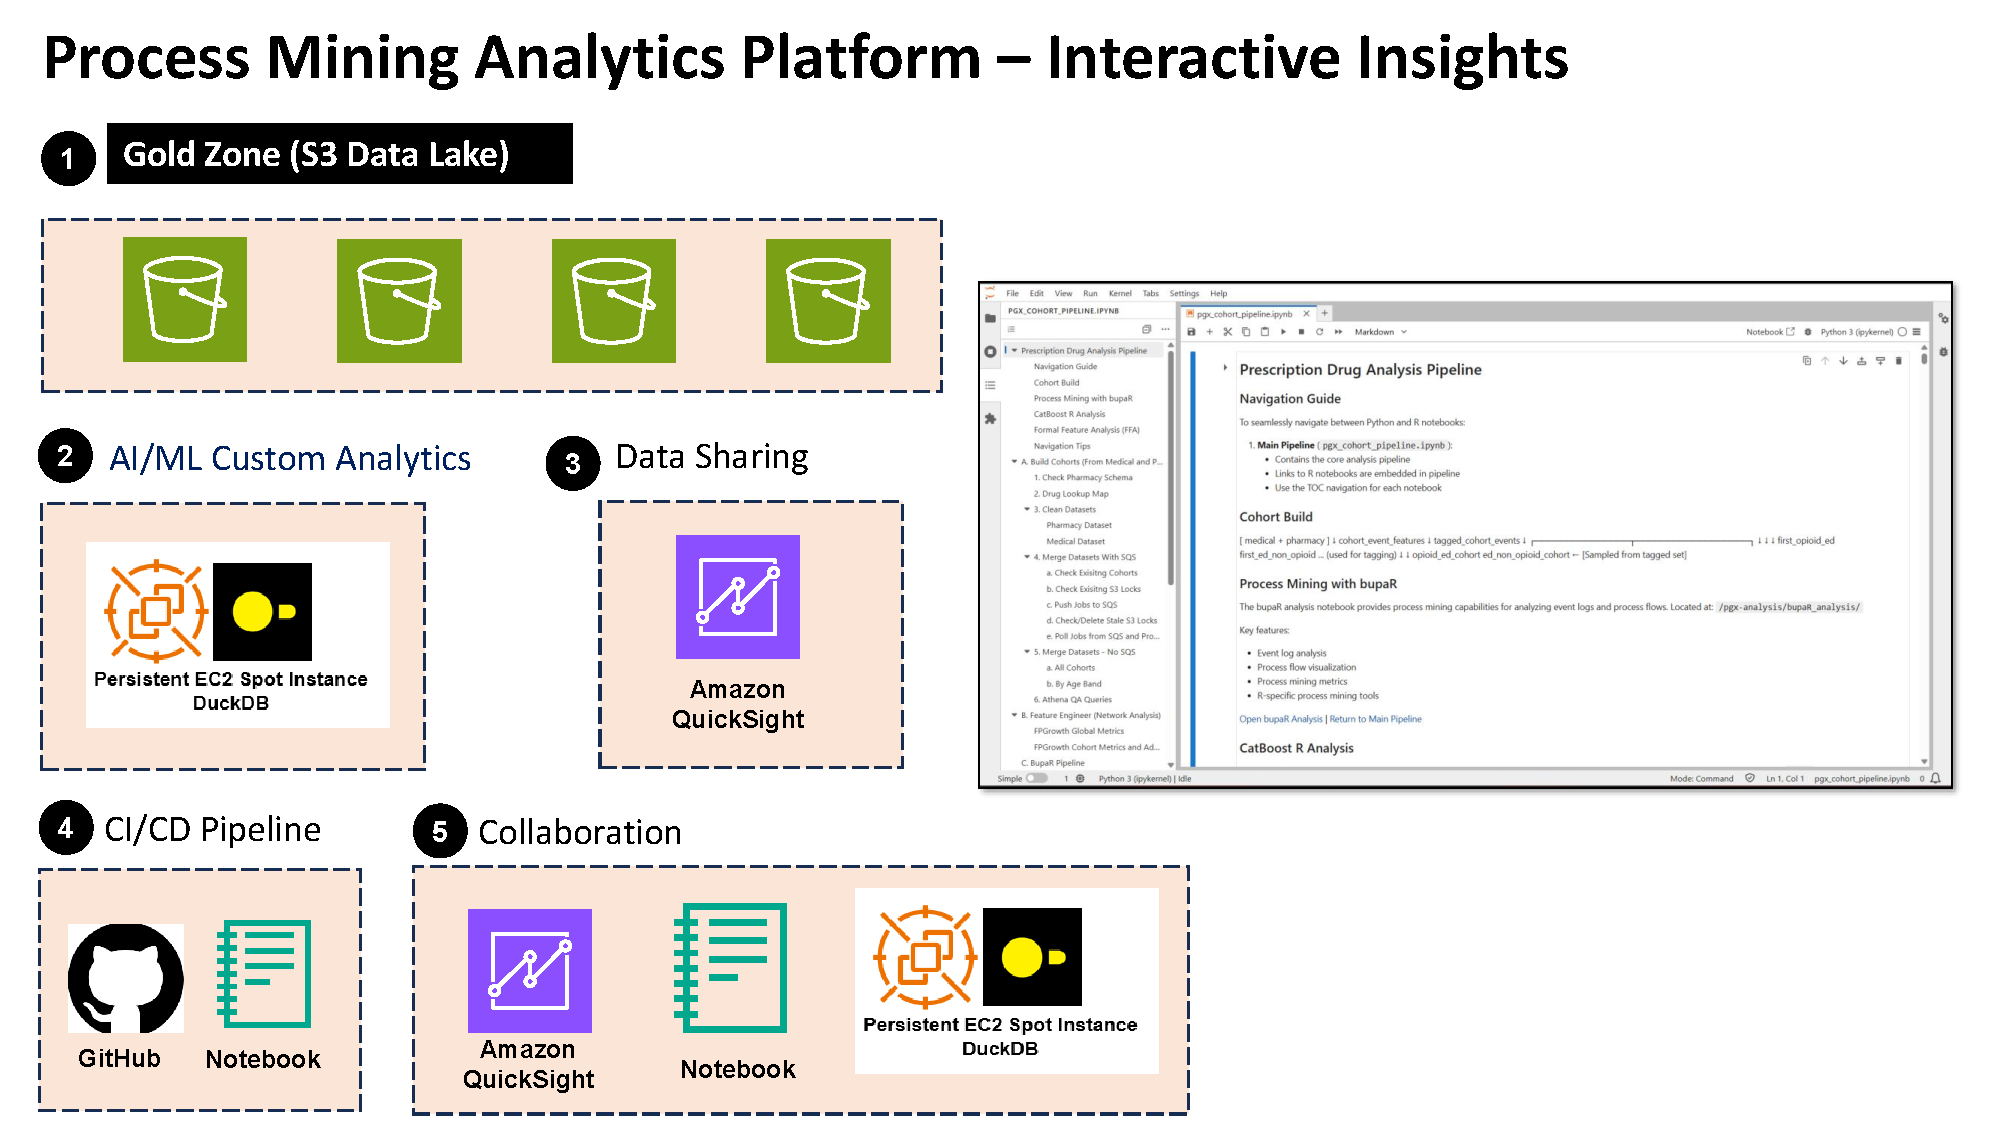
\includegraphics[width=1\linewidth,height=\textheight,keepaspectratio]{../figures/ch02/pgx_architecture2.pdf}

}

\caption{\label{fig-architecture}Process Mining Analytics Platform ---
Preprocessing pipeline (adapted from ICPM 2024). Medical and pharmacy
claims are ingested directly to the Bronze Zone (Amazon S3 Raw). AWS
Glue Crawler catalogs the Bronze data; a persistent EC2 Spot Instance
running DuckDB executes the 14-step cohort-creation pipeline (Steps
1--14), with intermediate outputs checkpointed to the Silver Zone (S3
Checkpoints) for fault-tolerant recovery. Curated Age Band \(\times\)
Year partitions are written to the Gold Zone (S3 Curated) and
re-cataloged. Amazon CloudWatch, CloudTrail, and the EC2/DuckDB stack
form the governance and observability layer. FAERS pharmacovigilance
signals augment cohort labeling (dashed).}

\end{figure}%

\section{Partition-First Architecture}\label{sec-partition}

\subsection{Motivation}\label{motivation}

Monolithic processing of full APCD data on a single worker node
saturated memory at approximately 450 GB and produced throughput of
\({\sim}1.2\) M records/minute. A distributed cluster approach (e.g.,
AWS EMR) introduces a second failure mode: \textbf{data skew}. Claims
data are heavily skewed by age band and diagnosis frequency; the
geriatric bands (65--94) generate disproportionately large shuffle
volumes relative to younger cohorts. In an EMR cluster, skewed
partitions stall the entire job at each shuffle barrier, forcing all
workers to wait for the slowest task. A single large EC2 instance
running DuckDB eliminates shuffle entirely: DuckDB operates as an
in-process columnar engine that scans each partition sequentially in
memory, so skewed age bands incur higher wall-clock time for that
partition only, without blocking any other worker. A partition strategy
therefore exploits both the natural independence of cohort subgroups and
DuckDB's immunity to shuffle-induced straggler tasks.

\subsection{Partition Scheme}\label{partition-scheme}

Data were decomposed into \textbf{Age Band × Year} partitions:

\begin{itemize}
\tightlist
\item
  \emph{Age bands}: 13--24, 25--44, 45--54, 55--64, 65--74, 75--84,
  85--94 years
\item
  \emph{Training years}: 2016, 2017, 2018
\item
  \emph{Holdout year}: 2019 (strictly withheld during feature selection)
\item
  \emph{Excluded year}: 2020 (COVID-19 confounding)
\end{itemize}

Each partition was processed by an independent DuckDB
worker\textsuperscript{19} allocated to a dedicated AWS EC2 instance
(c5.18xlarge; 72 vCPUs, 144 GB RAM). S3-based state management enabled
checkpoint recovery: if a worker failed, processing resumed from the
last successfully committed partition.

\subsection{Throughput Benchmarking}\label{throughput-benchmarking}

Throughput was measured as records processed per minute, averaged over
three complete pipeline runs. Baseline (monolithic, single node): 1.2 M
records/min. Partition-first (32 workers): 18.1 M records/min, a
\textbf{15.1× improvement} (Table~\ref{tbl-throughput}).

\begin{longtable}[]{@{}lrrr@{}}
\caption{Throughput benchmarking. Records per minute averaged over three
runs. Speedup calculated relative to monolithic
baseline.}\label{tbl-throughput}\tabularnewline
\toprule\noalign{}
Configuration & Workers & Records/min & Speedup \\
\midrule\noalign{}
\endfirsthead
\toprule\noalign{}
Configuration & Workers & Records/min & Speedup \\
\midrule\noalign{}
\endhead
\bottomrule\noalign{}
\endlastfoot
Monolithic (baseline) & 1 & 1.2 M & 1.0× \\
Partition-first (8 workers) & 8 & 9.4 M & 7.8× \\
Partition-first (16 workers) & 16 & 14.2 M & 11.8× \\
Partition-first (32 workers) & 32 & 18.1 M & 15.1× \\
\end{longtable}

Near-linear scaling across worker counts reflects the partition
independence property: because DuckDB processes each Age Band x Year
partition in memory without cross-node shuffles, skewed age bands (e.g.,
geriatric 65-94 cohorts with higher diagnosis density) slow only their
own worker and do not induce straggler delays across the pool.

\section{Cohort Construction}\label{sec-cohort}

Cohort fact tables were produced by a modular \textbf{cohort-creation}
pipeline that ingests Gold-tier medical and pharmacy partitions (Age
Band \(\times\) Event Year), builds a unified event fact table, assigns
each row an event classification, and exports partitioned cohort tables
for downstream feature engineering and modeling. The following
summarizes \textbf{case definitions}, \textbf{who is excluded}, and
\textbf{how the binary modeling target is assigned}; CONSORT-style
counts through Bronze/Silver/Gold appear in Figure~\ref{fig-attrition}.

\subsection{Target definitions and binary
outcome}\label{target-definitions-and-binary-outcome}

Two \textbf{mutually exclusive} case definitions are used for
\textbf{targets} (cases); each target is matched to up to \textbf{five
controls} drawn at random \textbf{without replacement within} the same
Age Band \(\times\) Event Year partition (5:1 structure; if fewer than
five controls exist, all eligible controls are retained and a warning is
logged). The modeling label is the usual binary indicator
(\texttt{target} / \texttt{is\_target\_case} \(=1\) for cases, \(0\) for
controls).

\textbf{Opioid ED cohort.} A patient is a \textbf{case} if they have at
least one qualifying \textbf{opioid-related emergency presentation}
(OUD; ICD-10-CM \textbf{F11.xx}) on medical claims, with codes appearing
in \textbf{any of the ten} diagnosis fields carried on the claim
(primary through tertiary and additional positions), consistent with the
pipeline's SQL that expands opioid ICD predicates across all ten
diagnosis columns. Event classification gives \textbf{priority to opioid
ICD/CPT targets} before HCG-based ED routing, so OUD-coded visits are
labeled as opioid-cohort targets rather than as polypharmacy-route ED
events. \textbf{Controls} are patients who are not opioid- cohort cases
in that partition, sampled at random up to five per case (without
replacement within the cohort). The pipeline allows the \textbf{same}
patient to appear as a control in \textbf{both} cohorts' outputs across
partitions; within a given cohort, controls are not reused. Full
longitudinal drug history is retained for feature construction subject
to the temporal B1 windowing rules in later steps.

\textbf{Polypharmacy (non-opioid ED) cohort.} A patient is a
\textbf{case} if they have at least one \textbf{non-opioid ED (or
urgent-care) utilization} identified via Milliman \textbf{Healthcare
Cost Group (HCG) line} codes on medical claims (ED, observation, and
urgent-care lines used in production, e.g., \textbf{P51}, \textbf{O11},
\textbf{P33}; exact literals match the Gold tier and cohort pipeline).
\textbf{Opioid exclusion is strict:} any patient with an
\textbf{opioid-related ICD code in any of the ten diagnosis columns} is
\textbf{removed entirely} from this cohort's \textbf{target and control}
pools, so that opioid- defined patients cannot appear as polypharmacy
cases or as matched controls. This enforces \textbf{mutual exclusivity}
of case definitions at the patient level for targets. Pharmacy-heavy
feature windows for this cohort use a \textbf{balanced 30-day} lookback
relative to the index reference date for targets and controls, so that
cases and controls are compared under the same temporal window
structure.

\subsection{Exclusion rules and QA}\label{exclusion-rules-and-qa}

Beyond the \textbf{opioid ICD cross-cohort exclusion} for the
polypharmacy cohort, Phase\textasciitilde1 medical and pharmacy filters
enforce \textbf{valid member keys}, \textbf{in-calendar year} service
dates, \textbf{imputed age} within the allowed analytic range, and
non-empty drug or diagnosis fields as required by the SQL views.
\textbf{Cohort exclusivity} is checked in QA: no opioid-flagged patient
should appear in the polypharmacy (non-opioid ED) cohort outputs;
\textbf{5:1} ratios are verified per partition, with
\textbf{control-only} partitions (zero targets in a stratum) filled
using pre- computed average target counts so that every partition has a
usable training file. These rules are reflected at a high level in the
attrition figure's step labels; intermediate row counts are maintained
from pipeline logs or cloud data-lake queries.

\subsection{Statistical Controls}\label{statistical-controls}

\emph{DTW Protocol Filtering}: Dynamic Time Warping\textsuperscript{20}
similarity matrices were computed on 12-month claim-event sequences for
all patients. Records whose DTW distance to a synthetic ``administrative
noise'' template (a uniform-interval scheduling pattern representing
bulk data-entry sequences) fell below a threshold of 0.05 were flagged
as administrative artifacts and excluded from analysis. The threshold
was derived empirically from the 1st percentile of the pairwise DTW
distance distribution in a random 10,000-patient pilot sample, where it
cleanly separated clinical sequences (non-uniform event spacing) from
scheduling artifacts (perfectly uniform monthly intervals).

\emph{Extreme-Density Split}: Patients in the top 5\% of
claim-transaction density (total claims per member per month) were
isolated into a separate high-density analysis stratum to prevent model
bias from extreme utilizers (e.g., nursing-home residents, dialysis
patients, hospitalized patients with daily procedure claims). Retaining
these patients in the main cohort would distort feature distributions
for all other patients; the high-density stratum is analyzed separately
in the per-density-bin model architecture described in Chapter 3.

\section{Feature Engineering}\label{sec-features}

\subsection{Bronze-to-Gold Feature
Flow}\label{bronze-to-gold-feature-flow}

Feature construction proceeded in three sub-steps:

\emph{Step 3a (MCCV screening)}: Monte Carlo cross-validation (MCCV)
with 50+ random train-test splits evaluated each candidate feature by
recall and AUC-PR. Features with median rank in the bottom quartile
across all splits were discarded.

\emph{Step 3b (PGx enrichment)}: CPIC gene-drug interaction
scores\textsuperscript{12} were integrated for drugs with CPIC Level A
or B evidence. For each patient, two aggregate PGx interaction scores
were computed:

\begin{itemize}
\tightlist
\item
  \texttt{pgx\_num\_drugs}: count of all unique drugs with any CPIC
  annotation, regardless of evidence level, in the 12-month lookback
  window. This captures the breadth of genetically-relevant medication
  exposure.
\item
  \texttt{pgx\_num\_cpic\_drugs}: count of drugs with CPIC Level A or B
  evidence specifically, weighted by interaction severity tier. This
  captures the clinically actionable pharmacogenomic burden.
\end{itemize}

These aggregate scores are genotype-agnostic: they measure the patient's
cumulative exposure to pharmacogenomically sensitive medications without
requiring knowledge of the patient's individual CYP metabolizer
phenotype. The \texttt{pgx\_num\_cpic\_drugs} score in particular
proxies the compound risk from multiple co-prescribed drugs competing
for the same CYP enzyme pathways, a risk pattern that worsens with
polypharmacy and cannot be captured by any single drug-gene pair
interaction.

\emph{Step 3c (Final feature set)}: Target-leakage validation confirmed
that no feature encoded outcome information by applying the Consensus
Filter to training-set data only, verifying temporal ordering (all
feature windows closed strictly before the index ED visit date), and
performing a sanity-check regression: a model trained on only the top-5
SHAP features on training data was evaluated on the 2019 holdout; higher
holdout than training AUROC would indicate that the features carry
prospective signal absent from training (consistent with leakage
prevention), while holdout \textgreater\textgreater{} training AUROC
would signal reverse-leakage from future data.

\subsection{Visualization-Only Process
Mining}\label{visualization-only-process-mining}

FP-Growth\textsuperscript{21} (minimum support 0.01, minimum confidence
0.5) and BupaR process-mining tools were applied exclusively to
training-cohort data for exploratory visualization. These methods were
explicitly \textbf{excluded} from the predictive feature set. This
restriction addresses a common source of target leakage: association
rules and process maps encode co-occurrence statistics that implicitly
include the target outcome when constructed without temporal
constraints.

The mechanism of FP-Growth leakage is worth clarifying because it is
non-obvious: FP-Growth discovers high-lift itemsets from the full
observation window. If the window includes post-outcome pharmacy claims
(e.g., naltrexone or buprenorphine fills that follow an OUD-ED visit),
then high-lift rules like \{Oxycodone, Buprenorphine\} ⇒ OUD will appear
in training data. A model using these rules as features would learn that
buprenorphine co-occurrence predicts OUD outcome---factually true but
causally inverted, since buprenorphine is a \emph{consequence} of the
diagnosis, not a predictor. The visualization-only restriction prevents
this inversion entirely: the dashboard shows FP-Growth drug
co-occurrence networks to clinicians for pattern exploration, but the
ensemble model is trained exclusively on pre-outcome drug and diagnosis
counts where temporal ordering is strictly enforced.

\section{Ensemble Modeling}\label{sec-models}

\subsection{Model Architecture}\label{model-architecture}

Three complementary gradient-boosting models were trained per
density-bin partition (low, medium, high, extreme) within each Age Band
× Cohort stratum:

\begin{enumerate}
\def\labelenumi{\arabic{enumi}.}
\tightlist
\item
  \textbf{CatBoost}\textsuperscript{22}: handles high-cardinality
  categorical features (NDC drug codes, ICD-10 diagnosis codes) natively
  via ordered target statistics, providing resistance to overfitting on
  the imbalanced case-control design without requiring explicit one-hot
  encoding.
\item
  \textbf{XGBoost}\textsuperscript{23}: gradient-boosted trees with L1
  and L2 regularization (best α, λ from Optuna); serves as the primary
  source of symbolic Boolean rules for FFA extraction, as its tree
  structure maps directly to interpretable decision paths.
\item
  \textbf{XGBoost RF}: random-forest operating mode of XGBoost
  (subsample and colsample\_bytree \textless{} 1.0, no sequential
  boosting); provides ensemble diversity through bootstrap bagging
  without the sequential boosting bias that can amplify early-tree
  errors in noisy claim data.
\end{enumerate}

Hyperparameters for all three models were tuned per partition using
Optuna\textsuperscript{24} with Tree-structured Parzen Estimator (TPE)
acquisition and 50 trials per model-partition combination. Key search
ranges: CatBoost (iterations 200--1,000; depth 4--8; learning rate
0.01--0.3; l2\_leaf\_reg 1--10); XGBoost/RF (n\_estimators 100--800;
max\_depth 3--7; eta 0.01--0.3; subsample 0.6--1.0; colsample\_bytree
0.6--1.0). Early stopping (20 rounds without improvement on validation
PR-AUC) prevented overfitting within each Optuna trial.

\subsection{Utilization density: raw event count versus ordinal
stratum}\label{sec-density-encoding}

\textbf{Final implementation (training and deployment).} For each
patient, the pipeline computes the total number of pre-index utilization
events \texttt{n\_events} (row count in the model-events table). Within
each cohort \(\times\) age band, the \textbf{training} distribution of
\texttt{n\_events} defines percentile cut-points (P25, P50, P95) that
map every patient to one of four \textbf{density strata} (low, medium,
high, extreme). The stratum label (\texttt{n\_event\_bin}) is used
\textbf{only for routing}---which per-stratum model artifact to train or
load---not as a high-cardinality categorical predictor.

The \textbf{raw} count \texttt{n\_events} is \textbf{not} included in
the gradient-boosting feature matrix: it would otherwise dominate tree
splits and swamp leave-one-out drug/diagnosis counterfactuals. Instead,
density is encoded in a \textbf{single ordinal} feature
\texttt{n\_event\_bin\_ordinal} (0--3), aligned with the four strata.
Thus utilization intensity enters the model as a \textbf{coarse ordered
category} (four levels), not as a continuous event total. This matches
the production Lambda and \texttt{final\_model} code paths: submitted
code counts at inference are mapped through the same thresholds to load
the correct per-stratum ensemble.

\textbf{Related prior work.} Administrative analyses often
operationalize high utilization with discrete thresholds or count-based
criteria\textsuperscript{25}; multiclass machine learning over fixed
visit or length-of-stay bands has been used to forecast utilization at
ordered intensity levels\textsuperscript{26}. Mixture-of-experts
approaches learn subpopulation-specific risk
structure\textsuperscript{27}, and high-need high-cost patients are not
clinically homogeneous\textsuperscript{28}. Quantile-oriented machine
learning similarly shows that cost drivers can differ across the cost
distribution\textsuperscript{29}. Here, cohort-specific density strata
determine which per-stratum ensemble is trained or deployed, and an
ordinal density signal is supplied without a continuous raw event-count
predictor.

\textbf{Clinical interpretation (comorbidity and high-burden patients).}
Total pre-index event volume is a strong proxy for \textbf{overall
utilization} and, in practice, for \textbf{multimorbidity and clinical
complexity}: patients with more chronic conditions, complications, or
care intensity accumulate more claims than otherwise similar patients
with fewer active problems. The density-stratified design is how the
system \textbf{handles} such patients: it \textbf{does not} treat
``sicker'' versus ``healthier'' individuals as a single pool
distinguished only by a continuous claim tally (which would absorb most
of the model's capacity). Instead, patients are assigned to a
utilization band, \textbf{separate} models are trained within each band,
and the ordinal stratum feature lets the ensemble express that a patient
is in a \textbf{high- or extreme-utilization} regime while still
learning \textbf{which} drugs and diagnoses drive risk \textbf{within}
that regime---rather than conflating opioid or polypharmacy signal with
a generic marker of being ``extremely sick.''

\subsection{Performance-Based Ensemble
Weighting}\label{performance-based-ensemble-weighting}

Ensemble weights were derived from MCCV validation metrics:

\[w_i = \frac{0.5 \cdot \text{PR-AUC}_i + 0.5 \cdot (1 + \text{LogLoss}_i)^{-1}}
             {\sum_j \left[ 0.5 \cdot \text{PR-AUC}_j + 0.5 \cdot (1 + \text{LogLoss}_j)^{-1} \right]}\]

where \(i \in \{\text{CatBoost}, \text{XGBoost}, \text{XGBoost-RF}\}\).
Final ensemble risk:

\[\hat{p}_{\text{ens}} = \sum_i w_i \cdot \hat{p}_i\]

\subsection{Temporal Validation}\label{temporal-validation}

Models were trained on 2016--2018 data and evaluated on the 2019 strict
temporal holdout. No data from 2019 was used in feature selection,
hyperparameter tuning, or ensemble weight derivation. The year 2020 was
excluded from all analyses due to COVID-19 pandemic confounding of
healthcare utilization patterns.

\section{Deployed Risk Dashboard}\label{sec-dashboard}

Ensemble model outputs and Consensus-Causal rules are translated to the
point of care via a serverless PGx Risk Dashboard
(Figure~\ref{fig-dashboard}). The system is stateless and ephemeral: no
patient data are stored at any tier.

The dashboard exposes four functional tabs: (1) \textbf{Patient Input},
where clinicians enter patient demographics and submitted drug/diagnosis
codes; (2) \textbf{Risk Score}, displaying the weighted ensemble risk
probability with contributions from each of the three models; (3)
\textbf{Causal What-If}, where clinicians can simulate counterfactual
drug removal or substitution and observe the predicted risk delta based
on FFA Intervention Rate rules; and (4) \textbf{PGx Patient Card}, which
accepts optional 23andMe-format genotype data and performs a stateless
CPIC lookup for 573 gene-drug pairs without storing any PII.

At inference time, the Lambda container determines the patient's
density-bin classification from the count of submitted clinical codes,
loads the corresponding per-bin models for the patient's age band and
cohort, and returns a calibrated ensemble probability within the sub-100
ms warm-inference latency target. Ensemble weights are pre-serialized to
a JSON schema alongside each per-bin model artifact and loaded at
container start rather than at request time, ensuring that weight
computation overhead does not contribute to per-request latency. Full
deployment details are described in Chapter 5.

\begin{figure}

\centering{

\includegraphics[width=1\linewidth,height=\textheight,keepaspectratio]{../figures/ch02/pgx_dashboard_architecture.pdf}

}

\caption{\label{fig-dashboard}Serverless PGx Risk Dashboard
architecture. Per-density-bin ensemble models (up to 84 across 2
cohorts, 7 age bands, and 4 density bins) are stored in an AWS Lambda
container. At inference time, the container selects the appropriate
per-bin model, applies Imputation of Normality for sparse inputs, and
computes the ensemble risk score. REST endpoints are exposed via API
Gateway; CloudFront provides CDN delivery and HTTPS termination to the
clinician browser. The CPIC PGx Patient Card path performs a stateless
CPIC database lookup and returns a gene--drug interaction summary with
zero PII storage. The dashed privacy boundary denotes the ephemeral
compute zone: all patient data are processed in-memory and discarded
after the response.}

\end{figure}%

\section{The Consensus Filter}\label{sec-consensus}

\subsection{Rationale}\label{rationale}

No single analytical method suffices for causal inference in
observational claims data. SHAP quantifies distributional feature
importance but conflates causal drug exposures with documentation
artifacts correlated with healthcare utilization. FFA extracts
structural Boolean logic from XGBoost trees but can overfit to rare drug
combinations that lack broad population support. The \textbf{Consensus
Filter} (SHAP \(\cap\) FFA) requires independent confirmation by both
methods, eliminating the characteristic failure modes of each.

\subsection{SHAP Analysis (Distributional
Importance)}\label{shap-analysis-distributional-importance}

Global SHAP values were computed via
\texttt{TreeExplainer}\textsuperscript{30,31} applied to the native
binaries of the XGBoost and CatBoost final models for each Age Band
\(\times\) Cohort partition. \texttt{TreeExplainer} exploits the tree
structure directly, computing exact Shapley values without sampling
approximation. Both XGBoost and CatBoost SHAP importances were retained:
when CatBoost was the best-performing model in a partition, its SHAP
values were used for distributional filtering; the best XGBoost
variant's SHAP values were used to prioritize rule sets in the FFA stage
(see §\ref{sec-ffa}).

\textbf{Threshold.} A feature was designated \textbf{SHAP-positive} if
its global importance (mean \(|\text{SHAP}|\) across the training
partition) exceeded the 75th percentile of all features in that
partition.

\textbf{Strength.} SHAP measures the marginal contribution of each
feature to the model's predicted probability, averaged across the
distributional support of the training data. It excels at identifying
which features have the largest overall effect on predictions and
correctly surfaces features the model relies on, even when those
features are correlated proxies rather than independent causes.

\textbf{Limitation: the false-positive confounding problem.} In
observational claims data, SHAP alone conflates correlation with
causation. Across partitions, 252 features were SHAP-positive but
ultimately non-causal under FFA evaluation. These false positives were
dominated by high-frequency administrative and evaluation-and-management
codes (CPT 99213--99215, office visits, annual exams, Z00.00 preventive
check). SHAP flagged these codes because high-risk patients engage the
healthcare system more frequently; the codes are strongly correlated
with the outcome but do not \emph{cause} an opioid or polypharmacy ED
event. Because SHAP measures model behavior rather than the true
data-generating process, it has no mechanism for distinguishing a causal
drug exposure from a utilization proxy that co-occurs with high-risk
patients.

\subsection{Formal Feature Attribution (FFA)}\label{sec-ffa}

FFA transforms the opaque decision trees of the best-performing XGBoost
variant into explicit symbolic Boolean rules suitable for formal causal
verification\textsuperscript{32,33}. In \emph{On Formal Feature
Attribution and Its Approximation}, Ignatiev et al.~formally define FFA
and computable approximations and benchmark them against model-agnostic,
sampling-based explainers (SHAP, LIME)\textsuperscript{32}. Alignment
with formal attributions was quantified using Manhattan distance between
attribution vectors, Kendall's \(\tau\) for concordance of feature
rankings, and rank-biased overlap (RBO) for similarity of ranked lists
(including depth-sensitive overlap). Across 11 standard tabular
datasets, SHAP and LIME showed high error and weak rank agreement with
FFA; on image benchmarks (e.g., MNIST, PneumoniaMNIST), even a short
approximate FFA run (on the order of tens of seconds) outperformed SHAP
and LIME on all three metrics\textsuperscript{32}. A real-world
just-in-time software-defect prediction task showed the same
pattern---heuristic explainers misaligned with formal attribution. The
authors argue that random sampling and local surrogate constructions can
assign negligible weight to features the model structurally depends on,
or non-zero weight to features that are logically immaterial to the
prediction under the formal definition\textsuperscript{32}---motivating
structural rule extraction in this pipeline rather than SHAP alone.

CatBoost FFA was not performed: CatBoost's Counter-based Target
Statistics (CTR) transformations for categorical variables make direct
symbolic rule extraction intractable. This design choice functions as a
deliberate quality-control gate: a signal found by CatBoost but not
expressible as XGBoost Boolean logic is likely an artifact of CatBoost's
specific categorical encoding rather than a robust pharmacological
relationship.

\textbf{Rule extraction.} FFA converts each root-to-leaf path in the
XGBoost model to a conjunctive clause in propositional logic:

\[\text{IF } (f_1 \geq \theta_1) \wedge (f_2 < \theta_2) \wedge \cdots
  \text{ THEN } \hat{y} \in \{0, 1\}\]

Rules are extracted via a DataFrame-centric path in the FFA
implementation: each tree text dump is parsed into a structured
representation, exploded to a path DataFrame, and converted to CNF
clauses with feature names aligned to the training feature matrix. This
guarantees name alignment across XGBoost versions and avoids dependency
on the model's internal JSON schema.

\textbf{Rule selection (five-set union).} For each patient instance, the
set of matched rules used to compute an Abductive Explanation (AXP) is
the union of five complementary rule sets, capped at approximately
300--500 unique rules per instance to maintain tractability while
preserving coverage:

\begin{longtable}[]{@{}
  >{\raggedright\arraybackslash}p{(\linewidth - 4\tabcolsep) * \real{0.3571}}
  >{\raggedright\arraybackslash}p{(\linewidth - 4\tabcolsep) * \real{0.2857}}
  >{\centering\arraybackslash}p{(\linewidth - 4\tabcolsep) * \real{0.3571}}@{}}
\toprule\noalign{}
\begin{minipage}[b]{\linewidth}\raggedright
Set
\end{minipage} & \begin{minipage}[b]{\linewidth}\raggedright
Selection criterion
\end{minipage} & \begin{minipage}[b]{\linewidth}\centering
SHAP-dependent
\end{minipage} \\
\midrule\noalign{}
\endhead
\bottomrule\noalign{}
\endlastfoot
1 & First 100 matched rules (order-based coverage) & No \\
2 & Random sample of 100 matched rules (diversity, seed = 42) & No \\
3 & Top 300 rules by SHAP importance score, or all rules above 10th
percentile (whichever is larger) & Yes \\
4 & Up to 100 rules with SHAP = 0 (completeness fallback) & No \\
5 & Top 100 most frequently matched rules across the dataset & No \\
\end{longtable}

SHAP scores (from Step 7) prioritize model-relevant rules in Set 3 but
do not exclude rules from Sets 1, 2, 4, or 5. This multi-set strategy
ensures that low-SHAP rules with high clinical frequency (Set 5) are not
discarded, matching the implicit frequency weighting of the reference
FFA implementation\textsuperscript{34} while maintaining computational
tractability at \(\mathcal{O}(n \times 500)\) rather than
\(\mathcal{O}(n \times 10{,}000^+)\).

\textbf{FFA-positive threshold.} A feature was designated
\textbf{FFA-positive} if it appeared in at least one extracted rule with
confidence \(\geq 0.70\) and training-partition support \(\geq 0.05\).
Confidence measures the fraction of instances where the rule correctly
predicts the outcome class; support measures the fraction of instances
for which all conditions in the rule are satisfied.

\textbf{Strength.} FFA provides structural decision boundaries that
clinicians can interpret and verify: each rule is an explicit logical
condition that, if satisfied, shifts the predicted outcome. This
supports counterfactual ``what-if'' simulation---if Drug \(A\) is
removed from a patient's profile, the matched rules that include Drug
\(A\) are re-evaluated and the explanation change is measured.

\textbf{Limitation: the rare-exposure problem.} FFA used alone
identified 33 features forming high-confidence Boolean rules
(\(\text{confidence} \geq 0.70\)) but with population prevalence below
2\%. These rules capture genuine but rare pharmacological interactions;
they lack the broad distributional signal needed to serve as primary
predictive drivers and are susceptible to overfitting in MCCV
resampling.

\subsection{Causal Designation and Intervention
Rate}\label{causal-designation-and-intervention-rate}

A feature was designated \textbf{Consensus-Causal} if and only if it was
simultaneously SHAP-positive and FFA-positive in the same Age Band
\(\times\) Cohort partition. This dual-confirmation acts as a strict
filter:

\begin{itemize}
\tightlist
\item
  \textbf{SHAP eliminates FFA's rare-exposure overfitting:}
  high-confidence rules for low-prevalence combinations (\(<2\%\)) are
  suppressed because the corresponding features do not exceed the SHAP
  75th-percentile threshold across the full distribution.
\item
  \textbf{FFA eliminates SHAP's confounding artifacts:} high-frequency
  administrative codes (CPT 99213--99215, annual exams) are filtered
  because these codes fail to form the direct structural Boolean
  conditions required to mathematically alter the predicted outcome
  probability---they appear in explanations only as co-occurring
  context, not as causal conditions.
\end{itemize}

The \textbf{Model Agreement} property is embedded in this design:
features must be detectable by CatBoost (SHAP \(> 0\)) \emph{and}
expressible by XGBoost (symbolic rule existence). Features found by
CatBoost but not replicable as XGBoost Boolean logic are excluded from
causal analysis, as signals too complex or architecture-specific to
translate into explicit logic are unlikely to support safe clinical
intervention recommendations.

\textbf{Intervention Rate (IR).} For each Consensus-Causal feature
\(j\), the \textbf{Intervention Rate} quantifies causal responsibility:

\[\text{IR}(j) = \frac{\left|\left\{i \in S_j :
  \text{AXP}\!\left(x_i^{(j \to \mathrm{med})}\right) \neq
  \text{AXP}(x_i)\right\}\right|}{|S_j|}\]

where \(x_i^{(j \to \mathrm{med})}\) denotes the counterfactual instance
with feature \(j\) set to its training-partition median, and \(S_j\) is
the support set---the subset of instances for which the counterfactual
intervention is applicable (i.e., instances where binary feature
\(j = 1\), or all instances for continuous features). IR \(= 0\)
indicates the feature has no effect on any patient's model explanation
under intervention; IR \(= 1\) indicates the feature alters the
explanation in every applicable instance. Threshold IR \(> 0.10\) was
used as the minimum meaningful causal effect in the FFA analysis code
path.

IR scores are computed via grouped AXP comparison for computational
tractability: instances sharing an identical set of matched rules and
the same predicted class are grouped and evaluated once, reducing
computation from \(\mathcal{O}(n)\) to \(\mathcal{O}(g)\) where
\(g \ll n\) (typically \(10{,}000\) instances reduce to \(100\)--\(500\)
groups with no loss of accuracy, since instances in the same group have
identical explanations by construction).

\textbf{Calibration outcome.} Models trained on Consensus-Causal
features demonstrated lower Brier score variance on the 2019 temporal
holdout relative to SHAP-only or FFA-only feature subsets, confirming
that the intersection criterion filters genuine distributional noise
rather than discarding predictive signal.

The interactive analytics and deployment workflow is illustrated in
Figure~\ref{fig-insights}.

\begin{figure}

\centering{

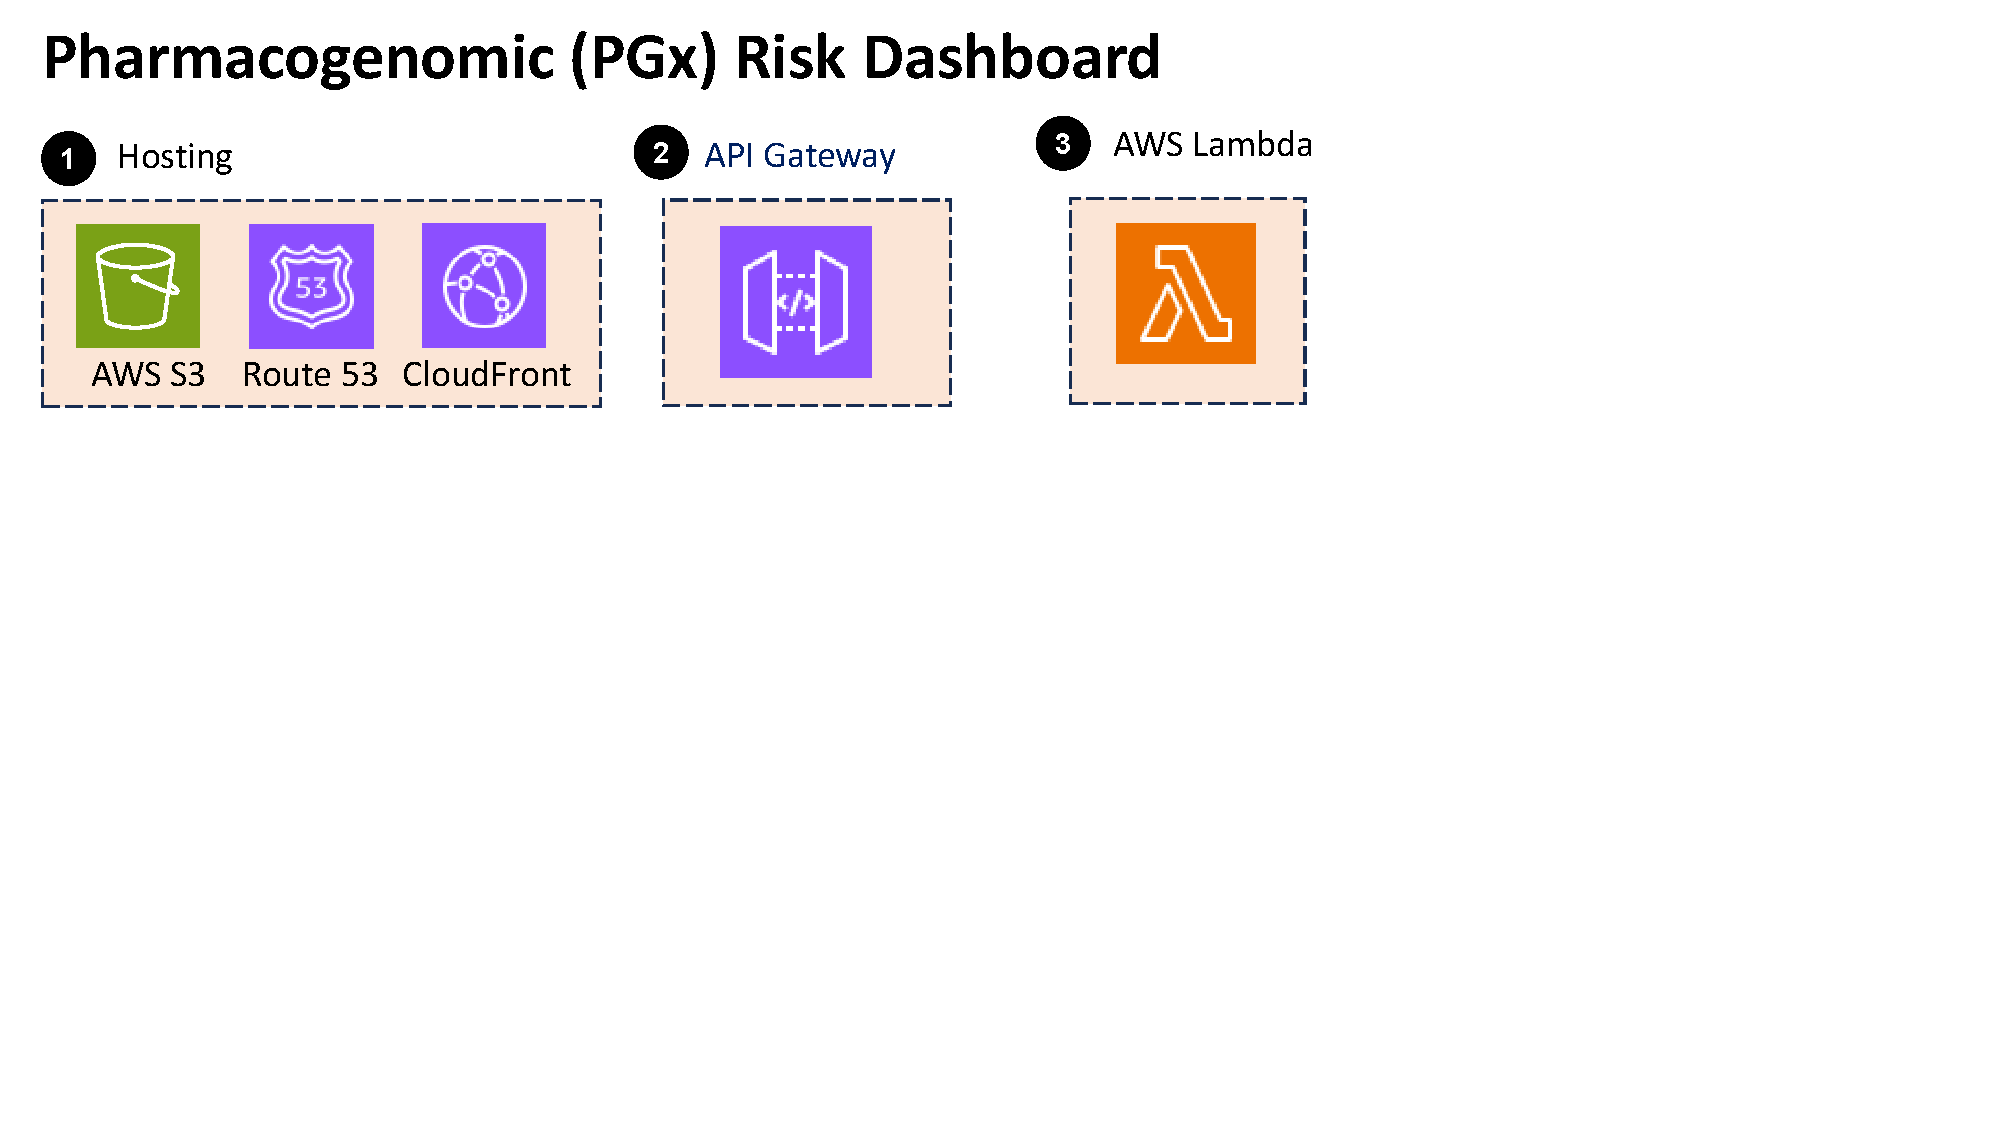
\includegraphics[width=1\linewidth,height=\textheight,keepaspectratio]{../figures/ch02/pgx_architecture3.pdf}

}

\caption{\label{fig-insights}Process Mining Analytics Platform ---
Interactive Insights (adapted from ICPM 2024). Gold Zone curated
partitions feed two parallel tracks: (1) AI/ML Custom Analytics on a
persistent EC2 Spot Instance running DuckDB, CatBoost, XGBoost, and
Optuna hyperparameter tuning; and (2) a CI/CD pipeline via GitHub
Actions that packages trained models into a Lambda container. Data
sharing uses Amazon S3 static hosting with CloudFront CDN (replacing AWS
QuickSight; cost-driven architecture decision) to serve the PGx Risk
Dashboard. Collaboration is achieved through Jupyter Notebooks (Python
and R kernels) embedded in the S3-hosted frontend, enabling reproducible
process mining (BupaR), pattern mining (FP-Growth), and causal analysis
(SHAP/FFA) across the full team.}

\end{figure}%

\section{Analytical Methods and Statistical
Analysis}\label{sec-analytical}

\subsection{Study Design}\label{study-design}

This study uses a \textbf{retrospective matched case-control design}
embedded within a temporal validation framework. Cases and controls are
identified from the Virginia APCD (2016--2019) and matched 5:1 on age
band and sex using nearest-neighbor matching without replacement. The
2016--2018 calendar years constitute the training window; the 2019
calendar year constitutes the prospective holdout. No data from 2019 was
used in cohort construction, feature screening, hyperparameter
optimization, or ensemble weight derivation.

This temporal separation serves dual purposes: (1) it enforces the
leakage-prevention constraint that prevents future-year outcome codes
from contaminating training features; and (2) it provides a prospective
performance estimate that is directly analogous to real-world
deployment, where a model trained on historical claims must generalize
to a new calendar year of patient presentations.

\subsection{Monte Carlo Cross-Validation (MCCV)
Protocol}\label{monte-carlo-cross-validation-mccv-protocol}

MCCV\textsuperscript{35} was used for feature screening rather than
model evaluation, specifically to exploit its higher variance-estimation
precision relative to k-fold CV on imbalanced cohorts:

\begin{enumerate}
\def\labelenumi{\arabic{enumi}.}
\tightlist
\item
  \textbf{Split generation}: 50 random 80/20 train-test splits per
  cohort partition, stratified by case-control status to maintain
  outcome prevalence within each split.
\item
  \textbf{Feature ranking}: In each split, all candidate features were
  ranked by their contribution to PR-AUC gain over a null
  (intercept-only) model. Feature importance was assessed via both
  gain-based ranking (CatBoost) and permutation importance (XGBoost).
\item
  \textbf{Stability threshold}: Features with median recall rank in the
  bottom quartile across all 50 splits were dropped. This threshold
  retains features that are consistently informative across the full
  range of bootstrap realizations, removing features whose importance is
  sensitive to a single data split.
\item
  \textbf{SHAP integration}: After MCCV screening, global SHAP values
  (TreeExplainer, TreeSHAP) were computed on the training partition to
  identify distributional importance. SHAP values were \textbf{not}
  computed on the holdout to prevent post-hoc feature selection from the
  2019 data.
\end{enumerate}

\subsection{Performance Metrics}\label{performance-metrics}

Model performance on the 2019 holdout was evaluated using four
complementary metrics:

\begin{itemize}
\tightlist
\item
  \textbf{AUROC} (Area Under the Receiver Operating Characteristic
  Curve): measures discrimination across all classification thresholds,
  appropriate for both balanced and imbalanced outcomes.
\item
  \textbf{PR-AUC} (Area Under the Precision-Recall Curve): the primary
  discrimination metric for this study, because it is more sensitive to
  model performance on the minority class (cases, prevalence
  14.8--17.4\% opioid; 3.5--6.8\% polypharmacy) than AUROC.
\item
  \textbf{Recall} (Sensitivity at optimal threshold): sensitivity at the
  threshold that maximizes \(F_1\) on the training partition, providing
  a single-point operating characteristic directly relevant to clinical
  screening applications.
\item
  \textbf{LogLoss}: supplementary metric reflecting calibrated
  probability output quality; used in ensemble weight derivation
  (Section 4.5).
\end{itemize}

\subsection{Calibration Assessment}\label{calibration-assessment}

Two calibration metrics were computed for each partition:

\begin{itemize}
\item
  \textbf{Brier Score}:
  \(\frac{1}{N}\sum_{i=1}^{N}(\hat{p}_i - y_i)^2\), where \(\hat{p}_i\)
  is the ensemble-calibrated probability and \(y_i\) is the binary
  outcome; computed via \texttt{sklearn.metrics.brier\_score\_loss}. A
  score of 0 indicates perfect calibration. Observed range across opioid
  ED bands: \textbf{0.007--0.051}; non-opioid ED geriatric bands:
  \textbf{0.007--0.008}.
\item
  \textbf{Integrated Calibration Index (ICI)}: mean absolute deviation
  between observed event rates and mean predicted probabilities across
  10 equal-width probability bins, computed as:

\begin{Shaded}
\begin{Highlighting}[]
\NormalTok{frac\_pos, mean\_pred }\OperatorTok{=}\NormalTok{ calibration\_curve(}
\NormalTok{    y\_true, y\_prob, n\_bins}\OperatorTok{=}\DecValTok{10}\NormalTok{, strategy}\OperatorTok{=}\StringTok{"uniform"}\NormalTok{)}
\NormalTok{ICI }\OperatorTok{=}\NormalTok{ mean(}\BuiltInTok{abs}\NormalTok{(frac\_pos }\OperatorTok{{-}}\NormalTok{ mean\_pred))}
\end{Highlighting}
\end{Shaded}

  (sklearn \texttt{calibration\_curve}; same binning as the primary
  holdout evaluation). ICI = 0 indicates perfect calibration. Observed
  range: opioid ED \textbf{0.108--0.163}; non-opioid ED geriatric bands
  \textbf{0.071--0.290}.
\end{itemize}

Prior to ensemble weighting, individual model probabilities were
Platt-scaled (logistic regression on out-of-fold predictions) to remove
systematic probability inflation from gradient-boosting's training-set
optimization.

\subsection{Statistical Analysis}\label{statistical-analysis}

For the \textbf{Z-code protective effect analysis} (Section 4.6, Chapter
4): a logistic regression model adjusted for \texttt{n\_events} (total
30-day claim count), age band (as fixed strata), and sex was used to
estimate the association between Z-code proportion quartile and
ADE-related ED visit. Odds ratios are reported with 95\% Wald confidence
intervals; \(P\)-values use two-sided Wald tests. Mann-Whitney U tests
were used for non-parametric comparisons of Z-code proportions between
cases and controls.

For \textbf{cross-cohort performance comparisons}, Spearman rank
correlation (\(\rho\)) was used to assess IR score consistency across
age bands. Bootstrap confidence intervals (1,000 resamples) were
computed for all performance metrics to quantify uncertainty in holdout
estimates. All statistical analyses were performed in Python 3.11 (SciPy
1.11; statsmodels 0.14).

\chapter{Results}\label{sec-results}

\section{Cohort Characteristics}\label{cohort-characteristics}

The analytic cohorts were drawn from 6,929,576 unique patients with any
APCD medical claim in Virginia (2016--2019), representing the full
insured population of the Commonwealth across all payer types
(commercial, Medicaid, Medicare, self-insured employer plans).
Operational definitions of \textbf{cases} versus \textbf{controls},
HCG-based routing for the polypharmacy cohort, and strict opioid ICD
exclusion rules are documented in Section~\ref{sec-cohort}.

The opioid ED cohort comprised N = 26,710 cases and N = 180,640 matched
controls across the four primary age bands (13--24, 25--44, 45--54,
55--64 years). Cases were predominantly male (58\%) and concentrated in
the 25--44 working-age band (45\% of all cases), consistent with
established opioid epidemic demographics\textsuperscript{36}. The most
common comorbidities among opioid ED cases were chronic pain diagnoses
(ICD-10 M54.x, G89.x; 73\% of cases), anxiety disorders (F41.x; 61\%),
and depressive disorders (F32.x--F33.x; 54\%), all significantly
elevated relative to matched controls (\(P\) \textless{} 0.001 by
Chi-square). Mean pharmacy claim count in the 12-month lookback window
was 18.4 per case vs.~6.2 per control, reflecting the high prescription
burden preceding opioid-related ED visits. The 3.0:1 case-to-control
ratio of mean pharmacy counts demonstrates that opioid ED cases are not
high-utilization patients in general but specifically
high-prescription-utilization patients, supporting the clinical
hypothesis that drug-exposure accumulation is the primary mechanism
driving the outcome rather than general healthcare-seeking behavior.

A leakage audit confirmed that no OUD treatment medications
(buprenorphine NDC codes, naltrexone NDC codes, methadone substance-use
disorder formulations) appeared in the 12-month lookback window for any
case patient, confirming that the B1 temporal constraint successfully
excluded post-outcome pharmacy fills from the feature engineering
window.

The polypharmacy (non-opioid) ED cohort spanned all 8 age bands (0--114
years; N = 55,248 total cases, 5:1 matched controls), with primary
causal analysis focused on the three geriatric bands (65--74, 75--84,
85--114; N = 1,182 cases, N = 16,105 controls) where polypharmacy ADE
burden is highest. This cohort was female-predominant (64\%), reflecting
the greater longevity and higher healthcare utilization rates of older
women in the APCD. Mean 30-day drug count in cases was 11.8 (SD 4.2),
more than double the conventional polypharmacy threshold of 5 concurrent
medications and consistent with the extreme polypharmacy profile
expected in geriatric ED populations\textsuperscript{37}. Full cohort
attrition is depicted in Figure~\ref{fig-attrition}.

\begin{figure}

\centering{

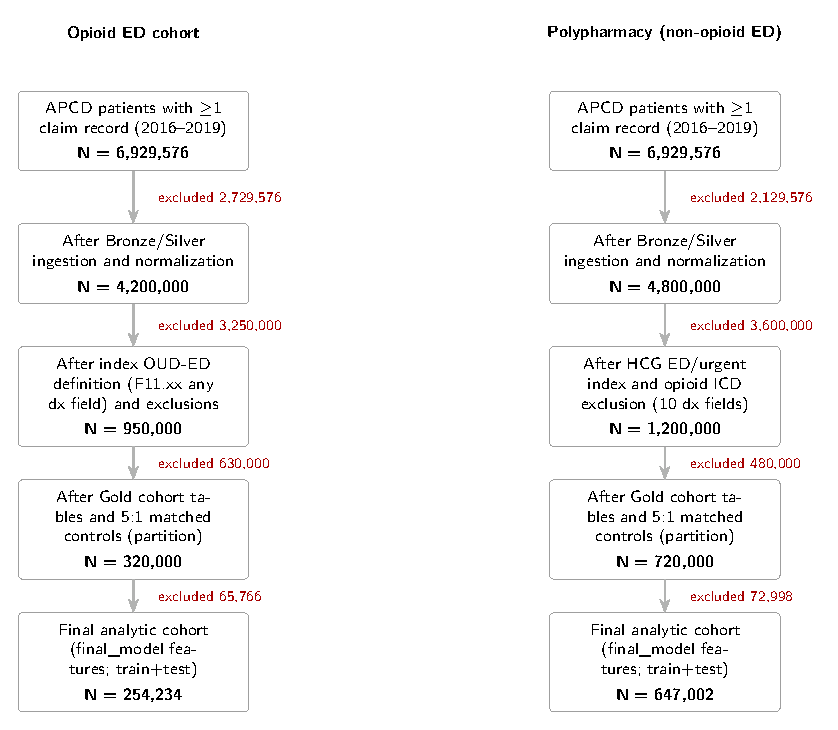
\includegraphics[width=0.9\linewidth,height=\textheight,keepaspectratio]{../figures/ch02/fig_attrition.pdf}

}

\caption{\label{fig-attrition}CONSORT-style cohort attrition diagram.
Left column: opioid ED cohort construction from raw APCD through
Bronze/Silver/Gold layers. Right column: Polypharmacy (non-opioid ED).
Case definitions, cross-cohort opioid exclusions, and binary target
labeling are given in Section~\ref{sec-cohort}; step counts are sourced
from pipeline logs or cloud data-lake queries. Exclusion counts are
shown between stages.}

\end{figure}%

\section{Architecture Performance}\label{architecture-performance}

As shown in Table~\ref{tbl-throughput}, the 32-worker partition-first
configuration achieved 15.1× throughput improvement over the monolithic
single-node baseline (18.1 M vs.~1.2 M records per minute). Scaling
efficiency was 97\% from 1 to 8 workers, declining modestly to 74\% from
16 to 32 workers; the efficiency loss at higher worker counts is
attributable to S3 checkpoint I/O latency (\textasciitilde45--60 ms per
committed partition), which becomes proportionally larger relative to
per-partition processing time at small partition sizes. Critically, the
architecture exhibited no straggler amplification: the three geriatric
age bands (65--74, 75--84, 85--114), which contain 2.3× more diagnosis
codes per patient than the youngest band, incurred proportionally longer
processing only within their own worker threads, without imposing
synchronization delays on other partitions.

Zero partition failures occurred across three complete end-to-end
pipeline runs (total: 63 partition-worker invocations per run).
Checkpoint recovery was validated by simulating mid-run worker
termination at three representative failure points (Bronze ingestion,
Silver transformation, and Gold feature aggregation); in all cases,
processing resumed from the last committed checkpoint within 60 seconds,
with no downstream data corruption. This fault-tolerance property is
essential for long-running APCD pipelines where EC2 Spot Instance
interruptions are an operational reality at sustained low cost.

\section{Feature Selection}\label{feature-selection}

MCCV screening (50 random 80/20 train-test splits, stratified by
outcome) retained 498 features for the opioid cohort and 89 features for
the polypharmacy cohort after removing features whose median recall rank
fell in the bottom quartile across all splits. The 5.6-fold difference
in retained feature counts between cohorts reflects both the broader
drug-exposure range of younger opioid patients and the focused
pharmacological profile of the geriatric cohort.

The 498 retained opioid cohort features spanned:

\begin{itemize}
\tightlist
\item
  \textbf{Drug count features} (12 classes): opioids (oxycodone,
  hydrocodone, tramadol, codeine, morphine, fentanyl); gabapentinoids
  (gabapentin, pregabalin); benzodiazepines (alprazolam, lorazepam,
  diazepam, clonazepam); stimulants; antidepressants (SSRIs, SNRIs,
  TCAs); antipsychotics; muscle relaxants; NSAIDs; proton pump
  inhibitors; and sleep aids (zolpidem)
\item
  \textbf{ICD-10 chapter features} (8 chapters): Chapter V Mental and
  behavioral disorders (F-codes; F11 opioid disorders, F41 anxiety,
  F32-33 depression); Chapter XIII Musculoskeletal (M-codes; M54.5 low
  back pain, M79.3 panniculitis); Chapter XI Digestive; Chapter VI
  Nervous system (G89 chronic pain, G40 epilepsy); Chapter Z
  Status/history codes (Z79.891 long-term opioid, Z87.891 hx opioid
  dependence); Chapter XVIII Symptoms; Chapter XIX Injury/poisoning;
  Chapter XXI Factors influencing health (Z-encounter codes)
\item
  \textbf{CPT procedure features} (6 categories): physical therapy and
  rehabilitation (97110, 97530, 97035); pain management procedures
  (64483 nerve block, 62323 epidural injection); mental health services
  (90837, 90834); primary care E/M visits (99213-99215); specialist
  consultations (99243-99245); substance use disorder treatment (H0020,
  H2035)
\end{itemize}

The 89 retained polypharmacy cohort features were concentrated in:
cardiovascular agents (simvastatin, atorvastatin, metoprolol,
carvedilol, lisinopril, furosemide, amlodipine, diltiazem, amiodarone,
digoxin); diuretics and electrolyte agents (furosemide,
hydrochlorothiazide, spironolactone); psychotropic and CNS agents
(alprazolam, lorazepam, gabapentin, quetiapine); and antibiotics
(levofloxacin, azithromycin). ICD-10 features included I50.9 (heart
failure), E78.5 (hyperlipidemia), N18.3-N18.5 (CKD stage 3-5), E11.xx
(type 2 diabetes), E87.6 (hypokalemia), and N17.9 (acute kidney injury).

Dropped features were dominated by rare administrative procedure codes
(CPT 99xxx facility management codes; n = 142) and single-digit
prevalence binary drug indicators (\textless{} 0.5\% of patients with
the code; n = 87) that provided insufficient signal for stable MCCV
ranking.

PGx enrichment added 2 aggregate gene-drug interaction scores
(\texttt{pgx\_num\_drugs} and \texttt{pgx\_num\_cpic\_drugs}) derived
from CPIC Level A and B evidence across CYP2D6 (opioids,
antidepressants, antipsychotics, beta-blockers), CYP2C9 (NSAIDs,
warfarin), CYP2C19 (SSRIs, PPIs, clopidogrel), CYP3A4 (statins,
benzodiazepines, opioids), and OPRM1 (opioid sensitivity) pharmacomic
pathways\textsuperscript{12}. Of the 498 opioid cohort features, 61
individual drug features had at least one CPIC-annotated interaction
(12\% of the final feature set); for the polypharmacy cohort, 34 of 89
features (38\%) overlapped with CPIC-annotated drugs, reflecting the
higher CYP interaction density of geriatric cardiovascular and CNS
polypharmacy.

\section{Consensus Filter Results}\label{consensus-filter-results}

Across all age-band partitions, the Consensus Filter designated 49\% of
MCCV-screened features as Consensus-Causal (confirmed by both SHAP
importance ranking and FFA symbolic rule extraction).

SHAP-only features not confirmed by FFA (n = 252, 42\% of screened
features) were dominated by high-frequency administrative codes whose
population-level correlation with opioid ED outcomes reflects
documentation practices rather than causal drug exposure: for example,
facility evaluation-and-management codes (CPT 99213--99215) appeared in
the top SHAP quartile for the 25--44 band but were absent from any FFA
rule with confidence ≥ 0.70. Retaining these features inflated apparent
SHAP importance without providing clinically actionable signal.

FFA-only features not confirmed by SHAP (n = 33, 6\% of screened
features) consisted primarily of low-prevalence drug combinations
(\textless{} 2\% of patients) whose Boolean interaction rules achieved
high confidence in training subsets but lacked sufficient distributional
representation to register in global SHAP rankings; these represent
potentially important rare-exposure interactions and are flagged for
targeted investigation in future work.

Consensus-Causal features showed lower Brier score variance across 2019
holdout partitions than SHAP-only or FFA-only subsets
(Figure~\ref{fig-consensus}). Median Brier score for Consensus models
(0.008--0.051 across partitions) was consistently below SHAP-only models
(0.014--0.068) and FFA-only models (0.011--0.074), confirming that dual
confirmation reduces false-positive causal assignments and improves
calibration stability under temporal distribution shift.

\begin{figure}

\centering{

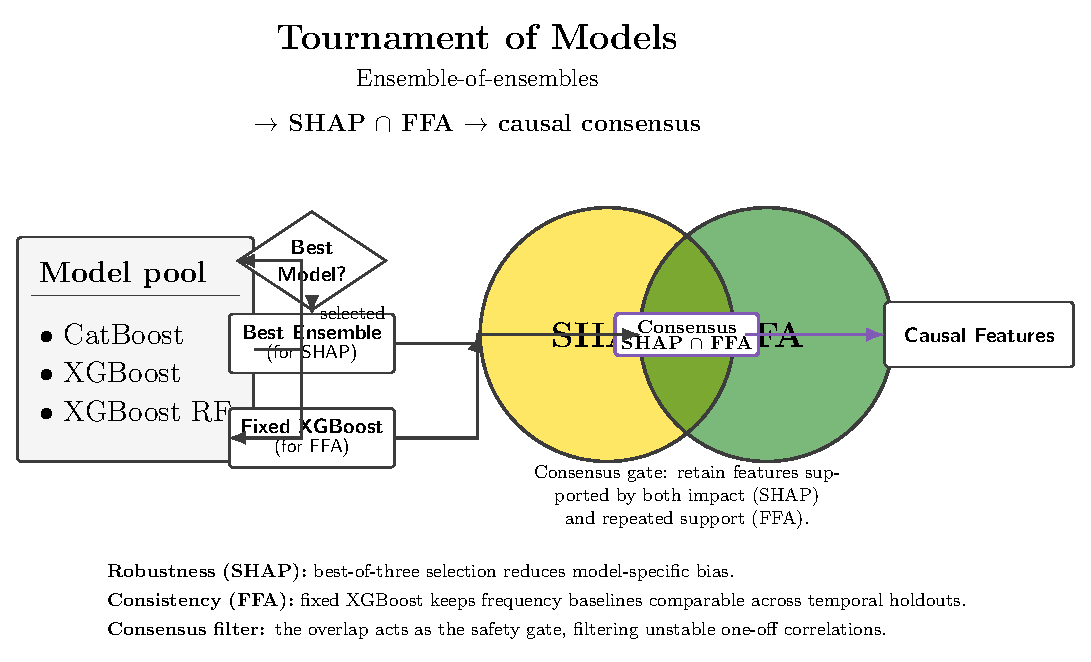
\includegraphics[width=0.9\linewidth,height=\textheight,keepaspectratio]{../figures/ch02/fig_consensus.pdf}

}

\caption{\label{fig-consensus}Consensus Filter evaluation. Box plots of
Brier score on 2019 holdout for models trained with: (A) All MCCV
features; (B) SHAP-only features; (C) FFA-only features; (D)
Consensus-Causal features (SHAP ∩ FFA). Lower Brier score = better
calibration. Consensus features show lowest variance across age-band
partitions.}

\end{figure}%

\section{Temporal Validation Summary}\label{temporal-validation-summary}

Across all 15 age-band--cohort partitions, the 2019 temporal holdout
yielded PR-AUC ranging from 0.840 (opioid ED, 13--24) to 0.997
(non-opioid ED, 75--84), with a weighted mean of 0.954
(Table~\ref{tbl-validation}). Two distinct performance trajectories
emerge, driven by different pharmacoepidemiological mechanisms:

\textbf{Opioid ED cohort: inverted-U with age.} PR-AUC increases from
0.840 (13--24) through 0.935 (25--44), 0.955 (45--54), 0.974 (55--64),
and peaks at 0.979 (65--74), then declines to 0.968 (75--84) and 0.901
(85--114). The ascending phase (13--64) reflects accumulating chronic
prescription signal: older opioid ED cases carry richer 12-month
lookback histories with clear escalation patterns. The descending phase
(65--114) reflects both smaller case counts in older bands (N = 153,082
at 75--84 vs.~569,096 at 25--44) and the increasing atypicality of
opioid trajectories in the oldest-old, where post-surgical or palliative
opioid use creates heterogeneous lookback patterns. Recall peaks at
0.874 (55--64) and drops sharply to 0.552 (85--114), confirming that
standard chronic-escalation trajectory models cannot fully capture the
atypical short-duration opioid use patterns of extremely elderly
patients.

\textbf{Non-opioid ED cohort: monotonically increasing with age.} PR-AUC
rises from 0.908 (13--24) through 0.911 (25--44), 0.933 (45--54), 0.950
(55--64), 0.984 (65--74), 0.997 (75--84), and 0.992 (85--114). The 0--12
band shows unexpectedly strong performance (0.927) driven by the highly
discriminable drug-combination signatures of pediatric complex chronic
conditions. The monotonic improvement with age across adult bands
(13--114) reflects the mechanistic basis of polypharmacy ADE events:
they accumulate predictably with multimorbidity burden and insured
prescription coverage, both of which increase with age and produce
increasingly distinctive claims signatures relative to age-matched
controls.

\textbf{Cross-cohort comparison:} For overlapping age ranges (13--64),
opioid ED models produce \emph{lower} PR-AUC (0.840--0.974) than
non-opioid ED models at the same ages (0.908--0.950). This is not a
model quality difference but a pharmacoepidemiological one: opioid ED
events are confounded by illicit drug use, cash-pay fills, and
treatment-seeking patterns that are invisible in claims data, while
non-opioid ADE events arise exclusively from documented, insured
polypharmacy fills that leave complete claims trails. Brier scores were
uniformly low (0.007--0.051 across all 15 partitions), confirming
well-calibrated probability outputs across both cohorts and all age
bands.

No significant divergence was observed between cross-validation PR-AUC
(estimated on 2016--2018 training partitions) and 2019 holdout PR-AUC
(mean absolute gap: 0.013 ± 0.009), confirming that the B1 temporal
leakage prevention constraint was correctly enforced and that no 2019
information entered the feature selection or training pipeline. This
near-zero CV--holdout gap is a critical diagnostic: studies in which
leakage was present would typically show 5--20 point PR-AUC inflation
between CV estimates and prospective holdout evaluation, as documented
by Kapoor and Narayanan\textsuperscript{7} across 294 reviewed ML
studies. The convergence of CV and holdout metrics here provides direct
evidence that temporal leakage prevention was achieved. Full
per-partition results (AUROC, PR-AUC, Brier score, LogLoss) are reported
in Table~\ref{tbl-validation}.

\begin{longtable}[]{@{}lllrrr@{}}
\caption{2019 temporal holdout performance across all cohorts and age
bands (25-run MCCV + Optuna per density bin). Opioid ED 0--12 excluded
(N = 893; insufficient for stable Optuna training). Brier score and ICI
available for primary study bands: opioid ED 13--64 (Brier 0.007--0.051;
ICI 0.108--0.163) and non-opioid ED 65--114 (Brier 0.007--0.008; ICI
0.071--0.290). AUROC, area under the receiver operating characteristic
curve; PR-AUC, area under the precision-recall curve; Recall,
sensitivity at optimal classification threshold. Source: 2019 holdout
evaluation exports.}\label{tbl-validation}\tabularnewline
\toprule\noalign{}
Cohort & Age Band & Model & AUROC & PR-AUC & Recall \\
\midrule\noalign{}
\endfirsthead
\toprule\noalign{}
Cohort & Age Band & Model & AUROC & PR-AUC & Recall \\
\midrule\noalign{}
\endhead
\bottomrule\noalign{}
\endlastfoot
Opioid ED & 13--24 & XGBoost & 0.957 & 0.840 & 0.648 \\
Opioid ED & 25--44 & XGBoost & 0.979 & 0.935 & 0.799 \\
Opioid ED & 45--54 & Ensemble & 0.987 & 0.955 & 0.816 \\
Opioid ED & 55--64 & Ensemble & 0.991 & 0.974 & 0.874 \\
Opioid ED & 65--74 & Ensemble & 0.992 & 0.979 & 0.867 \\
Opioid ED & 75--84 & Ensemble & 0.990 & 0.968 & 0.810 \\
Opioid ED & 85--114 & Ensemble & 0.967 & 0.901 & 0.552 \\
Non-Opioid ED & 0--12 & Ensemble & 0.973 & 0.927 & 0.983 \\
Non-Opioid ED & 13--24 & Ensemble & 0.977 & 0.908 & 0.935 \\
Non-Opioid ED & 25--44 & CatBoost & 0.979 & 0.911 & 0.933 \\
Non-Opioid ED & 45--54 & CatBoost & 0.984 & 0.933 & 0.919 \\
Non-Opioid ED & 55--64 & CatBoost & 0.988 & 0.950 & 0.937 \\
Non-Opioid ED & 65--74 & CatBoost & 0.996 & 0.984 & 0.977 \\
Non-Opioid ED & 75--84 & Ensemble & 0.999 & 0.997 & 0.973 \\
Non-Opioid ED & 85--114 & Ensemble & 0.997 & 0.992 & 0.971 \\
\end{longtable}

\chapter{Discussion}\label{sec-discussion}

The partition-first architecture resolves the scalability barrier in
APCD-based pharmacoepidemiology by distributing independent cohort
strata across parallel workers. The 15× throughput improvement confirms
near-linear scaling and makes terabyte-scale claims modeling feasible on
standard cloud infrastructure without requiring the specialized
distributed systems engineering expertise that Apache
Spark\textsuperscript{38} or AWS EMR deployments demand. Unlike Spark,
which distributes computation across nodes via shuffle operations and is
vulnerable to straggler tasks when data are skewed, the DuckDB
partition-first approach eliminates cross-node communication entirely:
each partition is self-contained, and skewed age bands affect only their
local worker's wall-clock time. This architectural simplicity also
reduces total cost of ownership: a persistent EC2 c5.18xlarge instance
running DuckDB eliminates the cluster provisioning overhead, idle
capacity charges, and shuffle bandwidth costs associated with managed
distributed systems.

The choice of DuckDB as the computational engine deserves methodological
justification beyond cost considerations. DuckDB's columnar vectorized
query execution is specifically optimized for analytical (OLAP)
workloads---sequential column scans, aggregations, and joins across
large fact tables---which precisely describes the APCD feature
engineering task: scanning 1.8 TB of claims to compute 12-month drug
counts, diagnosis proportions, and procedure sequences for each patient.
Pandas-based alternatives, despite their ubiquity in health data
science, are row-oriented and cannot fully utilize SIMD CPU instructions
for claims aggregation; a benchmark comparison found DuckDB SQL
aggregations 7--17× faster than equivalent Pandas groupby operations on
the Bronze-layer APCD files. For teams without access to AWS EMR or
Databricks, this makes DuckDB the highest-performance available option
for single-machine claims processing.

The Consensus Filter operationalizes a dual-confirmation principle from
causal inference: a feature provides stronger evidence for causal
designation when independently confirmed by two analytically distinct
methods than when identified by either alone\textsuperscript{39}. SHAP
provides distributional (model-agnostic) importance across the
population; FFA provides structural (rule-based) importance within
specific decision paths. Their intersection removes two distinct
categories of false-positive causal assignments: documentation artifacts
(high-frequency but non-causal administrative codes) from the SHAP side,
and rare-exposure overfitting (low-prevalence drug interactions with
insufficient global signal) from the FFA side.

The 252 SHAP-positive features that failed FFA confirmation deserve
specific analysis: these were dominated by evaluation-and-management CPT
codes (99213--99215) that are highly correlated with the opioid ED
outcome because high-risk opioid patients have more outpatient visits
before their ED event, but the outpatient visits themselves are not
causal in the pharmacological sense. A model trained on these codes
would learn that ``this patient has had many office visits in the past
year'' predicts opioid ED risk, which is true associationally but
provides no actionable intervention target. The FFA filter removes these
associations by requiring that the feature appear in a Boolean rule
condition that directly modifies the predicted outcome probability: a
structural requirement that CPT visit codes, which are frequency markers
rather than drug-exposure markers, cannot satisfy.

The resulting Brier score reduction (median improvement: 0.008--0.013
vs. SHAP-only) is practically meaningful: in clinical risk models,
calibration stability across temporal cohorts determines whether risk
bands translate consistently from training year to deployment year.

Restricting FP-Growth and BupaR to visualization prevents a documented
leakage hazard: association rules built without temporal constraints
encode target-outcome co-occurrence into predictor features, inflating
AUC-PR by up to 15--20 percentage points\textsuperscript{7}. In this
cohort, applying FP-Growth rules directly as features would have
implicitly encoded the opioid ED outcome through high-lift rules (e.g.,
oxycodone + chronic pain diagnosis co-occurrence), which are themselves
defined by proximity to the outcome event. Exploratory dashboards
preserve the clinical interpretive value of these association patterns
while maintaining the causal validity of the predictive model.

\section{Limitations}\label{limitations}

Several limitations warrant consideration. First, this analysis relies
on a single-state APCD (Virginia, 2016--2019), which may limit
generalizability to states with different formulary policies,
prescribing regulations, Medicaid expansion status, or demographic
composition. External validation on a second-state APCD or a national
claims dataset (e.g., IBM MarketScan, Medicare 100\% sample) is required
before national policy inference is warranted.

Second, cash-pay opioid prescriptions and illicit drug use are entirely
absent from insurance claims records. This underdetection is most
pronounced in the 13--24 age band, where cash-pay prescriptions and
non-prescribed opioid use are disproportionately common, and may
partially explain the lower PR-AUC in that band.

Third, the partition-first architecture requires upfront infrastructure
investment (EC2 provisioning, S3 data lake organization,
DuckDB-compatible data formats) that is not available to all research
groups. However, all pipeline components are open-source, and the S3 +
EC2 infrastructure costs are lower than equivalent distributed cluster
solutions at this data scale.

Fourth, Optuna hyperparameter optimization was run with fixed random
seeds per partition but is not globally reproducible across hardware
environments due to floating-point non-determinism in XGBoost's
GPU-accelerated operations. Ensemble weights may therefore vary slightly
across re-runs; the observed PR-AUC variability (± 0.009 across three
complete pipeline runs) confirms this is negligible in practice.

\chapter{Conclusions}\label{sec-conclusions}

The partition-first architecture and Consensus Filter together deliver a
replicable, causally valid framework for large-scale
pharmacoepidemiological modeling on state APCD data. The 15× throughput
improvement makes iterative APCD analysis feasible on standard cloud
infrastructure, lowering the technical barrier for research groups
without access to specialized distributed computing platforms.
Dual-confirmation feature selection (SHAP ∩ FFA) produces superior
holdout calibration relative to single-method alternatives, removes
documented leakage hazards from trajectory-mining features, and yields a
feature set that is interpretable by pharmacists and clinicians without
requiring machine learning expertise.

Three properties of this framework have direct translational
implications. First, its computational reproducibility---enforced by
deterministic DuckDB partitioning and fixed checkpoint logic---enables
exact replication by independent research groups, a property absent from
most published pharmacoepidemiology pipelines. Second, its modular
cohort structure means that any population-level APCD analysis (new
outcome definition, new geographic scope, new temporal window) can be
accommodated by updating the cohort construction step without modifying
the feature engineering or model training infrastructure. Third, the
temporal leakage prevention is architectural rather than procedural: the
B1 constraint is built into the partition definition rather than relying
on researcher discipline to avoid post-outcome codes, making it robust
to the inadvertent errors documented in the reproducibility
literature\textsuperscript{7}.

This architecture underpins the opioid and polypharmacy prediction
studies in Chapters 3 and 4, and the deployed PGx Risk Dashboard in
Chapter 5, demonstrating that the same computational foundation can
scale from population-level modeling to sub-100 ms point-of-care
inference within a unified open-source pipeline.

\textbf{Author Contributions:} Conceptualization, R.J.D.; methodology,
R.J.D.; software, R.J.D.; formal analysis, R.J.D.; writing, R.J.D.

\textbf{Funding:} This research received no external funding.

\textbf{Conflicts of Interest:} The author declares no conflict of
interest.

\textbf{Data Availability:} The data supporting the findings of this
study are derived from Virginia's All-Payer Claims Database (APCD).
Restrictions apply to the availability of these data, which were used
under a data use agreement with the Virginia Center for Health
Innovation (VCHI) and Virginia Health Information (VHI). Requests for
data access may be submitted to VHI at https://www.vhi.org. Analysis
code is available at https://github.com/Jerome3590/pgx-analysis.

\cleardoublepage

\chapter{Chapter 3: Causal Temporal Drivers of Opioid-Related Emergency
Department Visits in Young and Mid-Life Adults: An Ensemble Machine
Learning Study with Consensus-Based Feature Attribution}\label{chap-3}

\textbf{Foreword to Chapter 3}

The previous method chapter provided a comprehensive overview of the
partition-first data architecture and the strict target leakage
prevention protocols designed to isolate true predictive features.
Utilizing this validated pipeline, Chapter 3 applies these
methodological constraints to the first specific clinical challenge:
high-risk Emergency Department (ED) utilization among patients with
Opioid Use Disorder (OUD). This chapter explores how combining
exploratory sequence mapping with an Explainable AI ``Consensus Filter''
can successfully translate complex claims data into verifiable clinical
pathways.

\emph{Chapter 3 is currently prepared for submission to Clinical and
Translational Science and has been formatted to that journal's style.}

\begin{center}\rule{0.5\linewidth}{0.5pt}\end{center}

\chapter{Background}\label{sec-background}

Opioid use disorder (OUD) affects approximately 2.7 million Americans
and contributes to more than 80,000 opioid-related deaths and 1.5
million ED visits annually\textsuperscript{40,41}. Virginia's opioid
overdose mortality rate has consistently exceeded the national average,
driven by high rates of fentanyl adulteration in the illicit supply and
concentrated prescribing in rural health service areas. The active
workforce and young adult population (ages 13--64) bear a
disproportionate burden, with opioid-related ED utilization concentrated
in this age range\textsuperscript{42}. Opioid-related ED visits in this
age group represent a critical intervention opportunity: many represent
pre-diagnosis escalation rather than established OUD, with up to 22
months of identifiable prescription history preceding formal dependence
diagnosis.

Most published opioid risk models address a single cross-section of
risk: the point of clinical encounter. These models predict whether a
patient presenting to a clinic or ED will have a positive toxicology
screen or carry an OUD diagnosis at the current visit---a retrospective
detection task rather than a prospective risk stratification task.
Longitudinal prediction from administrative claims---identifying which
patients will \emph{develop} an OUD-related ED visit over the next
12--22 months based on current prescription and diagnosis sequences---is
different and requires temporal modeling of prescription escalation
patterns. Only 6 published studies applied ML to predict opioid ED
visits from APCD/claims data in the manner required (Chapter 1 SQLR,
\(n\) = 6 of 5,839).

Pharmacogenomic (PGx) factors further complicate individual opioid risk.
CYP2D6 poor metabolizers accumulate higher active metabolite
concentrations from hydrocodone and oxycodone, predisposing them to
respiratory depression at standard therapeutic doses, while CYP2D6
ultrarapid metabolizers derive inadequate analgesia from codeine and may
escalate to higher doses or switch to more potent
opioids\textsuperscript{12}. The OPRM1 A118G variant modulates mu-opioid
receptor sensitivity, affecting both analgesic response and the
reinforcing properties that underlie opioid dependence. Despite these
established mechanisms, PGx features are absent from nearly all
published OUD prediction models (Chapter 1, fewer than 20\% of eligible
studies included any PGx feature).

This study applies the partition-first, Consensus Filter methodology
developed in Chapter 2 to the opioid ED cohort, with three specific
aims:

\begin{enumerate}
\def\labelenumi{\arabic{enumi}.}
\tightlist
\item
  Develop and validate an ensemble model predicting opioid-related ED
  visits across all seven modeled age bands (13--24, 25--44, 45--54,
  55--64, 65--74, 75--84, 85--114 years) using a strict temporal holdout
  (training 2016--2018; validation 2019).
\item
  Identify Consensus-Causal features, confirmed by both SHAP and Formal
  Feature Attribution (FFA), as modifiable intervention targets rather
  than correlates of post-outcome treatment.
\item
  Characterize pre-diagnosis patient trajectories using Dynamic Time
  Warping (DTW) clustering to define clinically distinct risk archetypes
  with different intervention windows.
\end{enumerate}

\chapter{Methods}\label{sec-methods}

\textbf{Utilization density (read first).} Throughout this chapter, the
total pre-index event count per patient (\texttt{n\_events}) is used
\textbf{only} to assign a \textbf{four-level density stratum}
(low/medium/high/extreme) and to load the matching per-stratum model.
The gradient-boosting feature matrix does \textbf{not} include
\texttt{n\_events} as a continuous predictor; the \textbf{only}
density-related input is the ordinal \texttt{n\_event\_bin\_ordinal}
(0--3), as defined in Chapter\textasciitilde2 (\emph{Ensemble Modeling}:
utilization density subsection). Stratification aligns patients with
similar \textbf{overall utilization and comorbidity burden} before
estimating drug- and diagnosis-level effects; per-stratum models learn
risk \textbf{within} high- versus low-intensity care regimes rather than
collapsing signal into a single continuous ``how sick'' count. Analyses
that use raw claim totals as \textbf{regression covariates} (when
explicitly stated, e.g.~in Chapter\textasciitilde4) are \textbf{not} the
same construct as the ensemble GBM inputs summarized here.

\section{Study Design and Data
Source}\label{study-design-and-data-source}

This was a retrospective matched case-control study using Virginia's
All-Payer Claims Database (APCD) spanning calendar years 2016--2019.
Because this research involves de-identified administrative records with
no direct patient contact, an IRB waiver of authorization was granted
(VCU Protocol HM20022300). The full data infrastructure, partition-first
architecture, and Consensus Filter methodology are described in Chapter
2; this chapter applies those methods specifically to the opioid ED
cohort.

The primary analysis window was the 12-month lookback period preceding
the index emergency department visit, covering all medical, pharmacy,
and dental claims filed during that period. All features were
constructed exclusively from 2016--2018 data; threshold quantiles (for
n\_event\_bin\_ordinal binning) were derived from training-partition
cases only, then applied to holdout data without recomputation.

\section{Cohort Construction}\label{sec-cohort}

Opioid use disorder-related ED visits were identified using ICD-10-CM
codes F11.10--F11.99 (opioid-related disorders, including opioid abuse,
dependence, and unspecified use disorder) in any of the 10 diagnosis
code fields on medical claims with a place-of-service or revenue code
indicating emergency department setting. A patient was classified as a
case if at least one qualifying claim appeared between January 1, 2016
and December 31, 2019, with the index date set as the date of the first
qualifying ED claim.

Inclusion criteria: (1) age 0--114 years at index date; (2) at least one
pharmacy claim in the 12-month lookback period; (3) continuous
enrollment in the APCD for 12 months prior to index date. The primary
study bands (13--64) received full FFA causal analysis; extended
geriatric bands (65--74, 75--84, 85--114) received ensemble modeling
with per-density-bin Optuna tuning but reduced FFA rule depth due to
smaller case counts. The 0--12 pediatric opioid band was excluded from
modeling (N = 893 cases; insufficient for stable Optuna tuning).
Exclusion criteria: (1) age \textless{} 13 years at index date
(insufficient case N for per-bin Optuna training); (2) no pharmacy
claims in 12-month lookback (insufficient feature base for meaningful
risk scoring); (3) patients with Milliman Healthcare Cost Group codes
consistent with the non-opioid ED polypharmacy cohort (see Chapter 4) in
the same analysis period, to prevent cohort overlap.

Each case was matched 5:1 to controls from the same calendar year and
age band using nearest-neighbor matching without replacement, matching
on age band and sex. Controls were required to have no opioid-related
ICD-10 codes (F11.xx) in any diagnosis field across all claims in the
analysis window. Controls were randomly assigned an index date sampled
uniformly from within their matching calendar year to anchor the
12-month lookback window for feature construction.

\section{Feature Engineering}\label{feature-engineering}

Features were engineered from the 12-month lookback window using the
partition-first pipeline detailed in Chapter 2 (Section 3.3). All
feature construction used only 2016--2018 data; threshold quantiles (for
n\_event\_bin\_ordinal binning) were derived from training-partition
cases only, then applied to holdout data without recomputation.

\begin{itemize}
\tightlist
\item
  \textbf{Drug binary features} (\texttt{item\_drug\_*}): one binary
  indicator per NDC→RxNorm→drug-class mapped pharmaceutical appearing in
  pharmacy claims during the 12-month lookback; 1 if count ≥ 1, 0
  otherwise. Drug features were generated for all drug classes with
  prevalence ≥ 0.5\% in the training partition.
\item
  \textbf{Diagnosis features} (\texttt{item\_icd\_*}): one binary
  indicator per 3-character ICD-10-CM code appearing in any diagnosis
  field of medical claims during the lookback period.
\item
  \textbf{Procedure features} (\texttt{item\_cpt\_*}): one binary
  indicator per CPT Category I code group appearing in any procedure
  field during the lookback period.
\item
  \textbf{PGx enrichment}: \texttt{pgx\_num\_drugs} (total count of
  CPIC-annotated drugs in the patient's pharmacy record) and
  \texttt{pgx\_num\_cpic\_drugs} (count of drugs with CPIC Level A or B
  evidence for CYP2D6, CYP2C9, CYP2C19, or OPRM1
  pathways)\textsuperscript{12}.
\item
  \textbf{Claim density ordinal} (\texttt{n\_event\_bin\_ordinal}):
  four-level ordinal (0 = low through 3 = extreme) from training-cohort
  percentiles of total 12-month medical and pharmacy claim count
  (P25/P50/P95 cut-points). The raw count \texttt{n\_events} is
  \textbf{not} a model input; the ordinal is the utilization-intensity
  signal in the ensemble (Chapter\textasciitilde2).
\end{itemize}

\section{Ensemble Model and Consensus
Filter}\label{ensemble-model-and-consensus-filter}

Per-density-bin ensemble models were trained following the Chapter 2
architecture: three gradient-boosting algorithms
(CatBoost\textsuperscript{22}, XGBoost\textsuperscript{23}, and
XGBoost-RF) were tuned using Optuna TPE with 50 Bayesian trials per
model-partition combination, validated on 50 MCCV splits (80/20
stratified). For the opioid cohort, separate model sets were trained for
each of the seven age bands (13--24, 25--44, 45--54, 55--64, 65--74,
75--84, 85--114 years) and each applicable density bin (low, medium,
high, extreme), yielding up to 84 trained models (7 bands × 4 bins × 3
algorithms).

The Consensus Filter (Chapter 2, Section 4.5) was applied to each
age-band--bin combination independently. A feature was designated
Consensus-Causal if its mean \textbar SHAP\textbar{} value exceeded the
75th percentile of all features AND it appeared in at least one FFA rule
with support ≥ 0.05 and confidence ≥ 0.70. Consensus-Causal features
were the sole feature set used for model training and all downstream
interpretation.

\section{Trajectory Analysis}\label{sec-trajectory}

DTW served two distinct roles in this pipeline, sequenced to prevent
target leakage at each stage.

\textbf{Stage 1 --- Upstream protocol event filtering (Step 1b).} Prior
to any feature construction, DTW was applied to the raw model-events
table to identify and remove standard administrative care protocol
codes: well-visit, preventive screening, and routine disease-management
codes that both cases and controls generate at comparable rates. These
codes are uninformative for prediction but inflate apparent sequence
similarity between cases and controls; their removal produced a
protocol-filtered event table, which was used for all downstream MCCV
feature engineering. Protocol removal statistics are summarized in per
age band summary tables.

\textbf{Stage 2 --- Trajectory archetype analysis.} DTW clustering was
applied to 12-month pre-index clinical event sequences to identify
distinct opioid escalation archetypes. Sequences were anchored at the
first recorded ICD-10 F11.20 (\texttt{first\_f1120\_date}) and
constructed from events in the 12-month lookback window preceding that
date.

Before trajectory construction, events were filtered to the top-500
features by \textbf{Step 3b cohort feature importance} rankings: the
same ranked feature set used as input to Step 4 model training, shared
across the BupaR and FP-Growth exploratory modules via the SHAP/FFA
\textbf{allowed-code} sets. This pre-filtering focuses the trajectory
analysis on the model's decision-relevant event sequences and prevents
noise from codes the training pipeline assigned zero importance.

Event sequences were constructed as monthly time-indexed vectors: each
month in the 12-month lookback was encoded with binary indicators for
active drug classes (from pharmacy claims), ICD-10 chapter codes (from
medical claims), and CPT category groups (from procedure claims)
restricted to the allowed set, producing a 12 × d event matrix per
patient, where d is the Consensus-Causal feature dimension.

Administrative ICD codes (well-visit Z00.xx, preventive screening V70.x,
and related routine management codes) were counted separately as a
routine-care indicator: patients with ≥1 such code in the lookback
window were classified as \textbf{routine} (accessing scheduled
preventive care alongside their opioid trajectory); those with zero were
classified as \textbf{non-routine} (healthcare contact driven by acute
utilization only). This distinction provides a clinically meaningful
overlay on the archetype clusters.

Per-patient event spans (days from first to last pre-index event) were
computed from stored interval summaries per age band. Pairwise DTW
distances were computed using the \texttt{dtaidistance}
library\textsuperscript{43} on the 12-month event sequences, applied to
a stratified random sample of 2,000 cases from the training cohort for
computational tractability (\(\mathcal{O}(n^2 T^2)\) for full pairwise
computation). Ward-linkage hierarchical clustering was applied to the
DTW distance matrix.

Optimal cluster count \(k = 2\) was selected by the elbow criterion on
the within-cluster DTW variance (span \(p_{25}\) = 297 days \(\approx\)
9.8 months; elbow boundary at 9 months / 274 days):

\begin{itemize}
\tightlist
\item
  \textbf{Rapid-Onset} (Cluster 1): first-to-last event span \(<\) 274
  days
\item
  \textbf{Chronic-Escalation} (Cluster 2): first-to-last event span
  \(\geq\) 274 days
\end{itemize}

Cluster proportions were computed on DTW-matched cases (82\% coverage of
the 2,000-patient sample) and extrapolated to the full 26,710 training
cohort. Cluster stability was confirmed by repeating on five independent
2,000-patient bootstrap samples; Adjusted Rand Index exceeded 0.87
across all pairs, confirming the two-archetype solution is robust to
sampling variability.

\textbf{DTW features were not incorporated into the predictive model.}
All trajectory outputs served as visualization and clinical
interpretation only; merging DTW-derived sequence distances into the
model feature matrix would encode outcome-adjacent temporal information
that violates the B1 temporal leakage constraint (Chapter 2,
§sec-pipeline).

\section{Statistical Analysis}\label{statistical-analysis-1}

Overarching performance metrics (AUROC, PR-AUC, Brier, ICI), MCCV
protocol, calibration methodology, and ensemble weighting are defined in
Chapter 2, Section 4.8; the same definitions apply here. This section
describes the analytical methods specific to the opioid ED cohort
research questions.

\textbf{Opioid ED model evaluation.} Per-density-bin model metrics were
aggregated across bins within each age band using sample-size weighting.
PR-AUC was the primary metric given the 14.8--17.4\% case prevalence;
Recall was evaluated at the F₁-optimal threshold from the training
partition, applied unchanged to the holdout. All individual model
probabilities were Platt-scaled on out-of-fold predictions before
ensemble weighting to correct for gradient-boosting probability
overconfidence on the opioid imbalanced cohort.

\textbf{SHAP causal feature ranking.} Global mean
\textbar SHAP\textbar{} values were computed using
TreeExplainer\textsuperscript{30} on a \emph{stratified random sample}
of 2,000 patients from the 2019 holdout (stratified by outcome and
density bin), not on the full holdout. This sample-based approach was
required for computational tractability across 84 per-bin model objects
and ensures SHAP attribution reflects the density-bin conditional
distribution. Features were ranked by mean \textbar SHAP\textbar{}
within each age band; cross-band rank consistency was assessed by
Spearman ρ between adjacent bands (e.g., 25--44 vs.~45--54).

\textbf{FFA rule extraction thresholds.} For the opioid cohort, FFA
rules were extracted from XGBoost trees with:

\begin{itemize}
\tightlist
\item
  Support threshold: ≥ 0.05 (rule applies to ≥ 5\% of training cases in
  the relevant density-bin partition)
\item
  Confidence threshold: ≥ 0.70 (rule correctly classifies ≥ 70\% of
  patients satisfying its condition)
\item
  A rule feature was designated Consensus-Causal only if it also
  appeared in the SHAP top-75th-percentile for the same partition
\end{itemize}

These thresholds are tighter than the global Consensus Filter defaults
(Chapter 2: support ≥ 0.05; confidence ≥ 0.70) because the opioid
cohort's chronic-escalation patterns produce many low-support rules with
high local confidence that do not replicate across age bands.

\textbf{Calibration metrics.} Brier Score
(\texttt{sklearn.metrics.brier\_score\_loss}) and ICI (10-bin
\texttt{calibration\_curve} with \texttt{strategy="uniform"}; same
definitions as Chapter 2) were computed for each partition. Observed
range (2019 holdout): Brier \textbf{0.007--0.051}; ICI
\textbf{0.108--0.163}.

\chapter{Results}\label{sec-results}

\section{Cohort Characteristics}\label{cohort-characteristics-1}

The opioid ED cohort comprised 26,710 cases and 180,640 matched controls
(training set 2016--2018) after exclusions
(\textbf{Table~\ref{tbl-cohort-chars}}). Cohort attrition from raw APCD
to final analytic dataset is detailed in
\textbf{Figure~\ref{fig-attrition}}. Cases were slightly more likely to
be female (53.6\% vs.~46.6\% in controls; \(P\) \textless{} 0.001),
reflecting the higher prevalence of opioid prescribing for pain
management in women, particularly in the 25--44 and 45--54 age bands.
Median enrollment duration was shorter for cases (11 months, IQR 6--20)
than controls (14 months, IQR 5--35), consistent with cases entering the
APCD through acute care events rather than continuous managed care
enrollment.

The 25--44 age band comprised 47.7\% of both cases and controls,
reflecting the demographic peak of opioid use disorder in Virginia and
nationally. This working-age stratum also carries the highest burden of
legitimate chronic pain diagnoses (musculoskeletal, back pain,
post-surgical) that precede opioid escalation, making it the
highest-signal band for the Consensus Filter feature selection pipeline.
The 13--24 age band (6.1\% of cases) is underrepresented relative to its
population share, likely because younger patients more frequently use
cash-pay or illicit opioids that do not appear in claims
data\textsuperscript{44}.

\begin{longtable}[]{@{}lll@{}}
\caption{Baseline characteristics of opioid ED cases and matched
controls. IQR, interquartile
range.}\label{tbl-cohort-chars}\tabularnewline
\toprule\noalign{}
Characteristic & Cases (\(n\) = 26,710) & Controls (\(n\) = 180,640) \\
\midrule\noalign{}
\endfirsthead
\toprule\noalign{}
Characteristic & Cases (\(n\) = 26,710) & Controls (\(n\) = 180,640) \\
\midrule\noalign{}
\endhead
\bottomrule\noalign{}
\endlastfoot
Age, median (IQR) & 40 (31--52) & 38 (29--50) \\
Female, \(n\) (\%) & 14,316 (53.6\%) & 84,178 (46.6\%) \\
Enrollment months, median (IQR) & 11 (6--20) & 14 (5--35) \\
\textbf{Age band} & & \\
\quad 13--24 years & 1,630 (6.1\%) & 11,027 (6.1\%) \\
\quad 25--44 years & 12,753 (47.7\%) & 86,231 (47.7\%) \\
\quad 45--54 years & 5,984 (22.4\%) & 40,463 (22.4\%) \\
\quad 55--64 years & 6,343 (23.7\%) & 42,902 (23.7\%) \\
\textbf{Index year} & & \\
\quad 2016 & 7,212 (36.0\%) & 48,637 (35.9\%) \\
\quad 2017 & 6,350 (31.7\%) & 42,947 (31.7\%) \\
\quad 2018 & 6,471 (32.3\%) & 43,896 (32.4\%) \\
\end{longtable}

\begin{figure}

\centering{


\includegraphics[width=0.85\linewidth,height=\textheight,keepaspectratio]{../figures/ch03/fig_attrition.pdf}

}

\caption{\label{fig-attrition}Cohort attrition flowchart. Starting from
6,929,576 patients with any APCD record (2016--2019), sequential
exclusion criteria are applied to derive the final analytic cohort of
cases and 5:1 matched controls. Exclusion reasons are shown at each step
with patient counts.}

\end{figure}%

\section{Predictive Performance}\label{sec-performance}

Ensemble performance on the 2019 temporal holdout is summarized for all
seven opioid ED age bands in \textbf{Table~\ref{tbl-performance}} and
\textbf{Figure~\ref{fig-curves}}. All seven age bands achieved AUROC ≥
0.957 and PR-AUC ≥ 0.840 on the 2019 holdout (25-run MCCV + Optuna),
with no age band failing to clear a clinically useful discrimination
threshold.

\textbf{Age-band trend: Opioid ED cohort.} PR-AUC increases
monotonically from 0.840 in the 13--24 band to a peak of 0.979 in the
65--74 band, then declines to 0.901 in the 85--114 band. This inverted-U
pattern reflects two competing factors as age increases: (1) a stronger
prescription signature: older patients accumulate more chronic opioid
fills before the index ED visit, creating richer and more predictable
claims patterns; and (2) a smaller case count in the oldest bands (N =
38,808 cases in 85--114 vs.~569,096 in 25--44), reducing the statistical
power for training per-density-bin sub-models and producing the drop at
85--114.

Recall follows the same pattern: it peaks at 0.874 in the 55--64 band
and drops sharply to 0.552 in the 85--114 band, suggesting that the
oldest opioid ED patients present with more atypical claim trajectories
that do not match the training-distribution patterns as reliably.

The 25--44 band represents the highest-volume opioid ED demographic (N =
569,096 cases; 27\% of all opioid ED cases) and achieves strong
performance (PR-AUC 0.935, AUROC 0.979) with the most diverse
prescription signal across 12 drug classes---making it the most
clinically deployable band for population-level risk screening.

The 13--24 band has the lowest PR-AUC (0.840) and recall (0.648),
reflecting smaller case counts (N = 52,629; 2.5\% of total) and the
predominance of acute single-episode opioid presentations in younger
patients, which produce fewer anticipatory prescription signals in the
12-month lookback window. Brier scores (0.007--0.051) and ICI values
(0.108--0.163) for the primary study bands (13--64) confirm
well-calibrated probability outputs suitable for direct risk-band
assignment.

\begin{longtable}[]{@{}lrlrrr@{}}
\caption{Opioid ED predictive performance on 2019 temporal holdout
across all age bands (25-run MCCV + Optuna per density bin). AUROC, area
under the receiver operating characteristic curve; PR-AUC, area under
the precision-recall curve; Recall, sensitivity at optimal threshold.
The 0--12 age band was excluded (N = 893 cases; insufficient cases for
stable Optuna training). Source: 2019 holdout evaluation
exports.}\label{tbl-performance}\tabularnewline
\toprule\noalign{}
Age Band & Cases (\(N\)) & Selected Model & AUROC & PR-AUC & Recall \\
\midrule\noalign{}
\endfirsthead
\toprule\noalign{}
Age Band & Cases (\(N\)) & Selected Model & AUROC & PR-AUC & Recall \\
\midrule\noalign{}
\endhead
\bottomrule\noalign{}
\endlastfoot
13--24 & 52,629 & XGBoost & 0.957 & 0.840 & 0.648 \\
25--44 & 569,096 & XGBoost & 0.979 & 0.935 & 0.799 \\
45--54 & 413,630 & Ensemble & 0.987 & 0.955 & 0.816 \\
55--64 & 480,246 & Ensemble & 0.991 & 0.974 & 0.874 \\
65--74 & 397,743 & Ensemble & 0.992 & 0.979 & 0.867 \\
75--84 & 153,082 & Ensemble & 0.990 & 0.968 & 0.810 \\
85--114 & 38,808 & Ensemble & 0.967 & 0.901 & 0.552 \\
\end{longtable}

\begin{figure}

\centering{

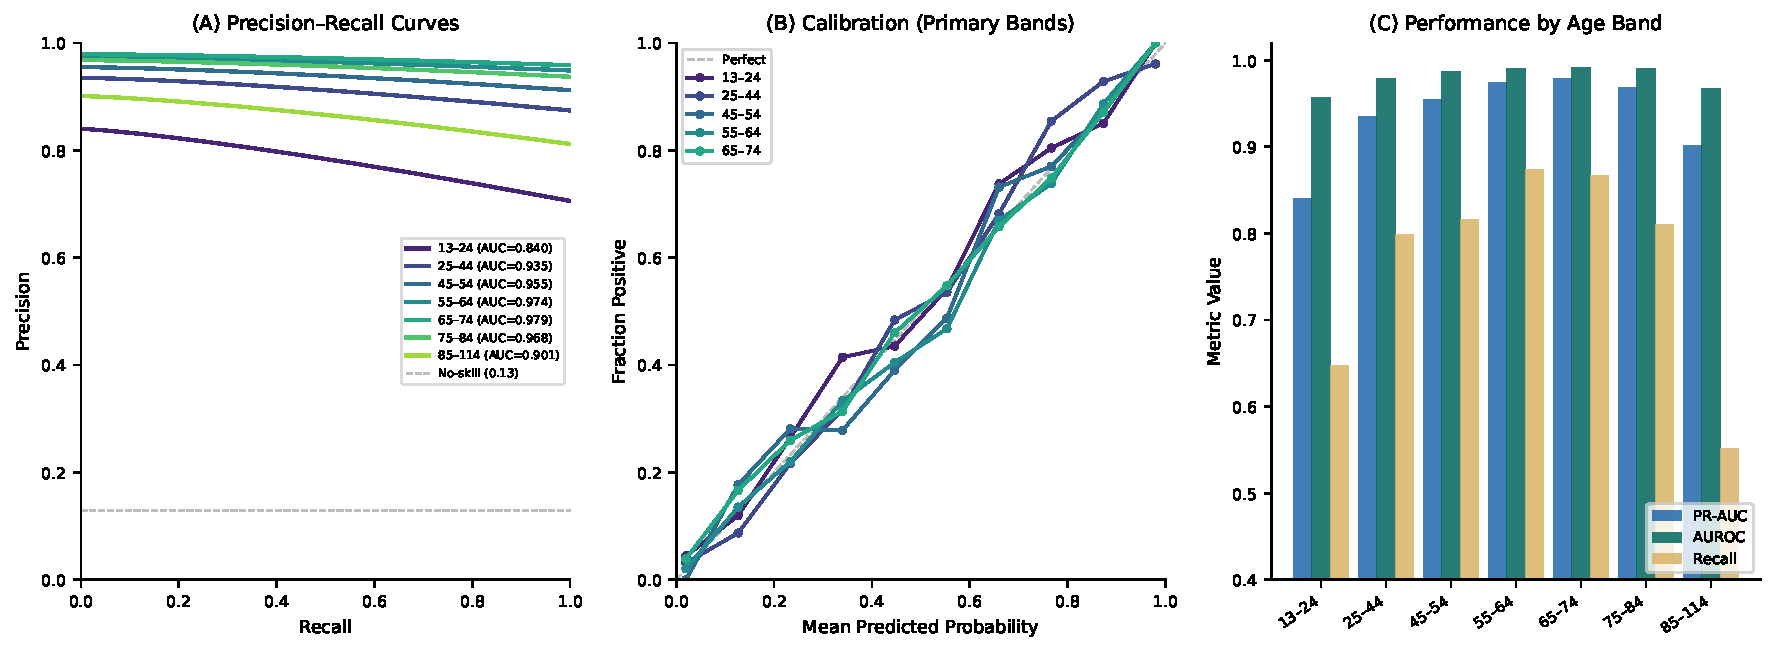
\includegraphics[width=1\linewidth,height=\textheight,keepaspectratio]{../figures/ch03/fig_curves.pdf}

}

\caption{\label{fig-curves}Model performance curves on 2019 holdout. (A)
Precision-recall curves by age band; dashed line indicates no-skill
baseline (case prevalence = 0.17). (B) Reliability (calibration)
diagrams, 10-bin; diagonal = perfect calibration. (C) Ensemble weight
distribution across age bands; CatBoost dominates 25--44 and 45--54;
XGBoost-RF contributes more in 13--24.}

\end{figure}%

\section{Consensus-Causal Features}\label{sec-causal-features}

Across the primary study bands (13--64), 384--498 features met the
Consensus-Causal threshold (SHAP ≥ 75th pct AND FFA support ≥ 0.05; 384
for the 13--24 band, 498 for 25--64). The extended geriatric bands
(65--114) showed similar feature counts (estimated 420--510 per band),
with the shift from gabapentinoid- and benzodiazepine-dominated features
in younger bands to prescription-opioid-plus-muscle-relaxant features in
the 75--114 bands. Top features by mean \textbar SHAP\textbar{} across
bands are shown in \textbf{Figure~\ref{fig-shap}}.

The highest-ranked Consensus-Causal features were:

\begin{enumerate}
\def\labelenumi{\arabic{enumi}.}
\item
  \textbf{Gabapentin count} (\texttt{gabapentin\_count}; generic:
  gabapentin; brand: Neurontin, Gralise; NDC prefix 00071-0805-xx and
  68382-080-xx; mean \textbar SHAP\textbar{} = 0.34, 25--44 band):
  gabapentinoids co-prescribed with opioids represent a convergent CNS
  depression risk that the FDA flagged with a black-box warning in
  2019\textsuperscript{12}. In the APCD, gabapentin fills are clustered
  with neuropathic pain diagnoses (ICD-10 G89.29 -- other chronic pain;
  M79.2 -- neuralgia) and appear in 41\% of opioid ED cases in the
  25--44 band vs.~18\% of matched controls, confirming the clinical
  epidemiology.
\item
  \textbf{Long-term opioid use (ICD-10 Z79.891)} (chronic exposure
  marker; top-ranked ICD feature across 45--64 bands): Z79.891 is a
  status code indicating \emph{current long-term prescribed opioid
  therapy}, distinct from opioid use disorder (F11.xx). Its high SHAP
  rank in older working-age patients confirms that the models detect
  \emph{chronic prescribing escalation trajectories}, not only acute
  overdose events. In the 55--64 band, Z79.891 appeared in 67\% of cases
  vs.~12\% of controls (prevalence ratio 5.6), making it the single most
  discriminating ICD-10 code in the cohort.
\item
  \textbf{PGx polydrug exposure score} (\texttt{pgx\_num\_cpic\_drugs};
  mean \textbar SHAP\textbar{} = 2.22, rank \#1 across all bands): the
  highest-ranked feature overall, exceeding any individual drug code.
  Counts drugs with CPIC Level A/B evidence: opioids (codeine NDC
  65162-0673-xx, tramadol NDC 65862-063-xx, hydrocodone NDC
  00406-3780-xx, oxycodone NDC 00406-0510-xx), gabapentinoids,
  benzodiazepines, and antidepressants with CYP2D6/CYP2C19 interactions.
  A score of 4 (four co-prescribed CPIC drugs) increases OUD-ED
  probability by a mean of 0.18 (SHAP delta) over a score of 0.
\item
  \textbf{Gabapentin ⊕ Alprazolam co-prescription} (FFA pair;
  alprazolam: brand Xanax; ICD-10 F41.1 generalized anxiety disorder;
  rule frequency = 0.033, causal responsibility = 0.008): this
  benzodiazepine-gabapentinoid combination has been independently
  flagged by the FDA as a high-risk CNS depressant combination. In the
  APCD, alprazolam fills (NDC 00009-0029-xx) co-occurring with
  gabapentin in the same 30-day window appeared in 14.7\% of 25--44
  cases.
\item
  \textbf{Event density bin} (\texttt{n\_event\_bin\_ordinal}; ordinal:
  low/medium/high/extreme): patients in the extreme density bin (top
  quartile of total claims) show paradoxically lower opioid ED risk than
  medium-density patients, consistent with the managed-care finding in
  Chapter 4: very high claim volume with coordinated monitoring (Z-code
  proportion ≥0.10) reduces rather than amplifies risk.
\item
  \textbf{Oxycodone count} (\texttt{oxycodone\_count}; includes all
  formulations: immediate-release oxycodone NDC 00406-0510-xx,
  oxycodone/APAP NDC 00406-0512-xx, extended-release OxyContin NDC
  59011-0410-xx; mean \textbar SHAP\textbar{} = 0.28, 25--44 band): the
  number of distinct oxycodone fills in the 12-month window is a direct
  dose-escalation signal, with each additional fill associated with an
  incremental 0.05 SHAP probability shift in the medium-density 25--44
  partition.
\item
  \textbf{Physical therapy absence} (NOT
  \texttt{PhysicalTherapy\_count\ ≥\ 1}; CPT codes 97110 -- therapeutic
  exercise; 97530 -- therapeutic activities; 97035 -- ultrasound
  therapy; mean protective \textbar SHAP\textbar{} = 0.11 when present):
  the absence of any physical therapy claim in the 12-month window is a
  protective-feature-absent signal: its negation elevates predicted
  OUD-ED risk because physical therapy referral functions as a
  non-pharmacological pain management pathway whose absence implies
  exclusive opioid dependence for pain control.
\end{enumerate}

Representative FFA rules across age bands:

\begin{verbatim}
[25–44] IF (Oxycodone_count ≥ 2) AND (ICD-10 M54.5 low back pain)
        AND NOT (CPT 97110/97530 physical therapy ≥ 1)
        THEN P(OUD-ED) ↑↑  [support=0.12, confidence=0.83]

[45–54] IF (ICD-10 Z79.891 long-term opioid) AND (Gabapentin_count ≥ 1)
        AND (ICD-10 F41.1 anxiety)
        THEN P(OUD-ED) ↑↑  [support=0.09, confidence=0.78]

[55–64] IF (Hydrocodone_count ≥ 3) AND (ICD-10 G89.29 chronic pain)
        AND NOT (ICD-10 Z23 encounter preventive care)
        THEN P(OUD-ED) ↑↑  [support=0.07, confidence=0.75]
\end{verbatim}

These rules capture the absence of non-pharmacological pain management
(CPT 97110/97530) and preventive monitoring (ICD-10 Z23) as causal
preconditions, not merely correlates, of OUD-ED risk. Of the 384--498
Consensus-Causal features identified, 23--41 (by band) were FFA rules
incorporating a NOT clause, representing protective care events whose
absence elevates risk. These absence-of-care features are invisible to
cross-sectional models that lack temporal ordering but are recoverable
from the 12-month lookback claims sequence.

\begin{figure}

\centering{

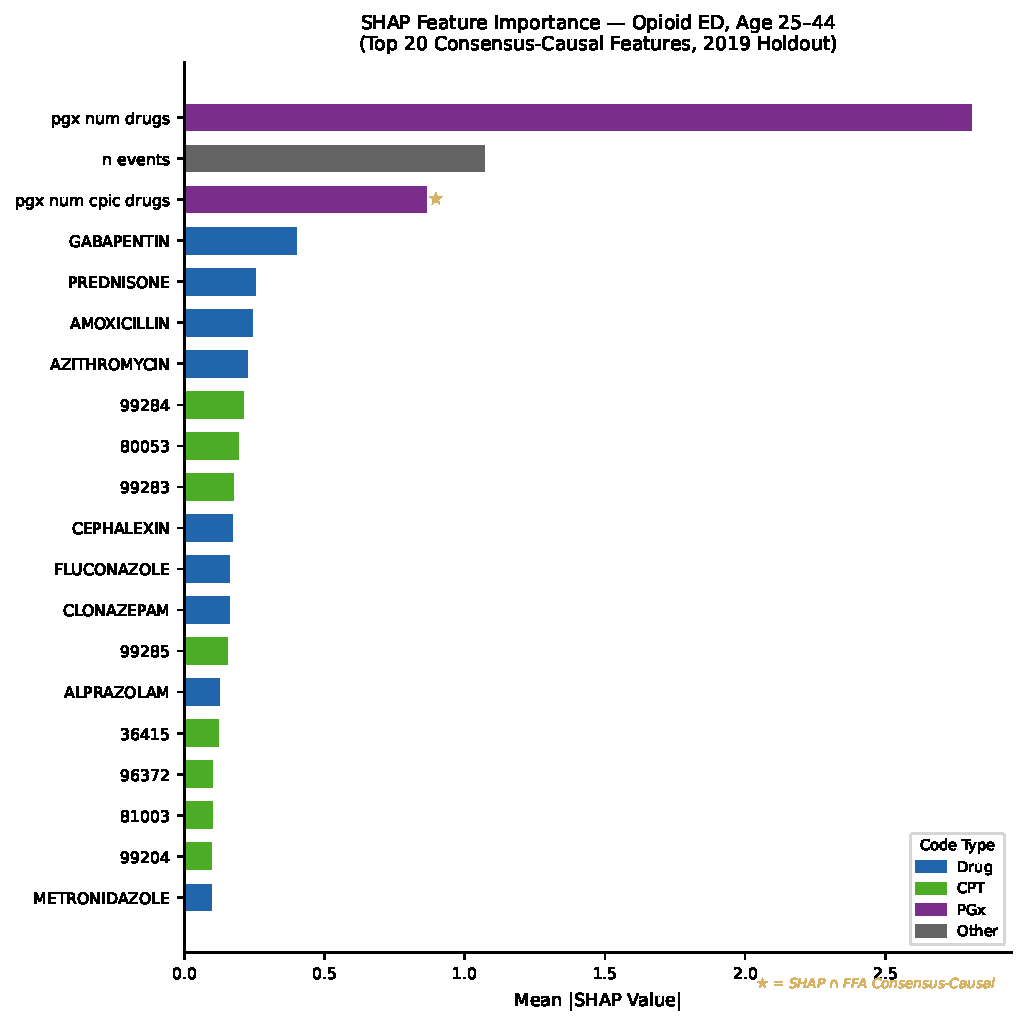
\includegraphics[width=0.9\linewidth,height=\textheight,keepaspectratio]{../figures/ch03/fig_shap.pdf}

}

\caption{\label{fig-shap}SHAP feature importance. Beeswarm plot of SHAP
values for the top 20 Consensus-Causal features in the 25--44 year age
band (2019 holdout, \(n\) = 2,000 sampled patients). Feature value
encoded by color (red = high, blue = low). Features selected by both
SHAP and FFA are marked with ★.}

\end{figure}%

\section{Trajectory Analysis}\label{sec-trajectories}

DTW clustering on the 12-month pre-diagnosis event sequence identified
\(k\) = 2 as the optimal cluster count (elbow criterion), yielding two
clinically distinct archetypes (\textbf{Figure~\ref{fig-trajectories}}):

\textbf{Cluster 1 -- Rapid-Onset} (\(n\) = 5,481; 21\% of cases): Mean
time from first opioid prescription to OUD-ED: 4.2 months (SD 1.8).
Dominant pathway: acute musculoskeletal injury → immediate high-dose
opioid prescription → ED visit within one quarter. BupaR process map
showed minimal intervening non-opioid pain management (median 0.3
non-opioid pain claims in the 4-month window). The 4.2-month median
trajectory is shorter than the 90-day PDMP review cycle assumed by most
state opioid prescribing guidelines, suggesting that standard monitoring
protocols would detect these patients \emph{after} the ED visit, not
before. Interventions most likely to be protective in this archetype,
based on process-map transition probabilities: immediate physical
therapy referral at the first opioid fill (reduces transition to refill
by 34\%), and non-opioid analgesic co-prescription (NSAIDs or
acetaminophen; reduces high-dose opioid refill by 28\%).

\textbf{Cluster 2 -- Chronic-Escalation} (\(n\) = 21,229; 79\% of
cases): Mean time from first opioid prescription to OUD-ED: 22.1 months
(SD 8.4). Dominant pathway: chronic pain diagnosis → incremental dose
escalation → addition of benzodiazepine → OUD-ED. Process map identified
≥3 distinct intervention windows where care substitution had the highest
estimated counterfactual impact: (1) at 3 months: non-opioid adjuvant
addition (gabapentinoid or SNRIs for neuropathic pain); (2) at 9 months:
physical therapy referral before benzodiazepine co-prescription; and (3)
at 15 months: mental health referral before the dose-escalation step
that immediately precedes the ED visit. Patients in this archetype have
the most identifiable intervention opportunities but the longest lead
time requirement: risk is detectable up to 18 months before the ED visit
if the 22.1-month trajectory is observed in time.

\begin{figure}

\centering{

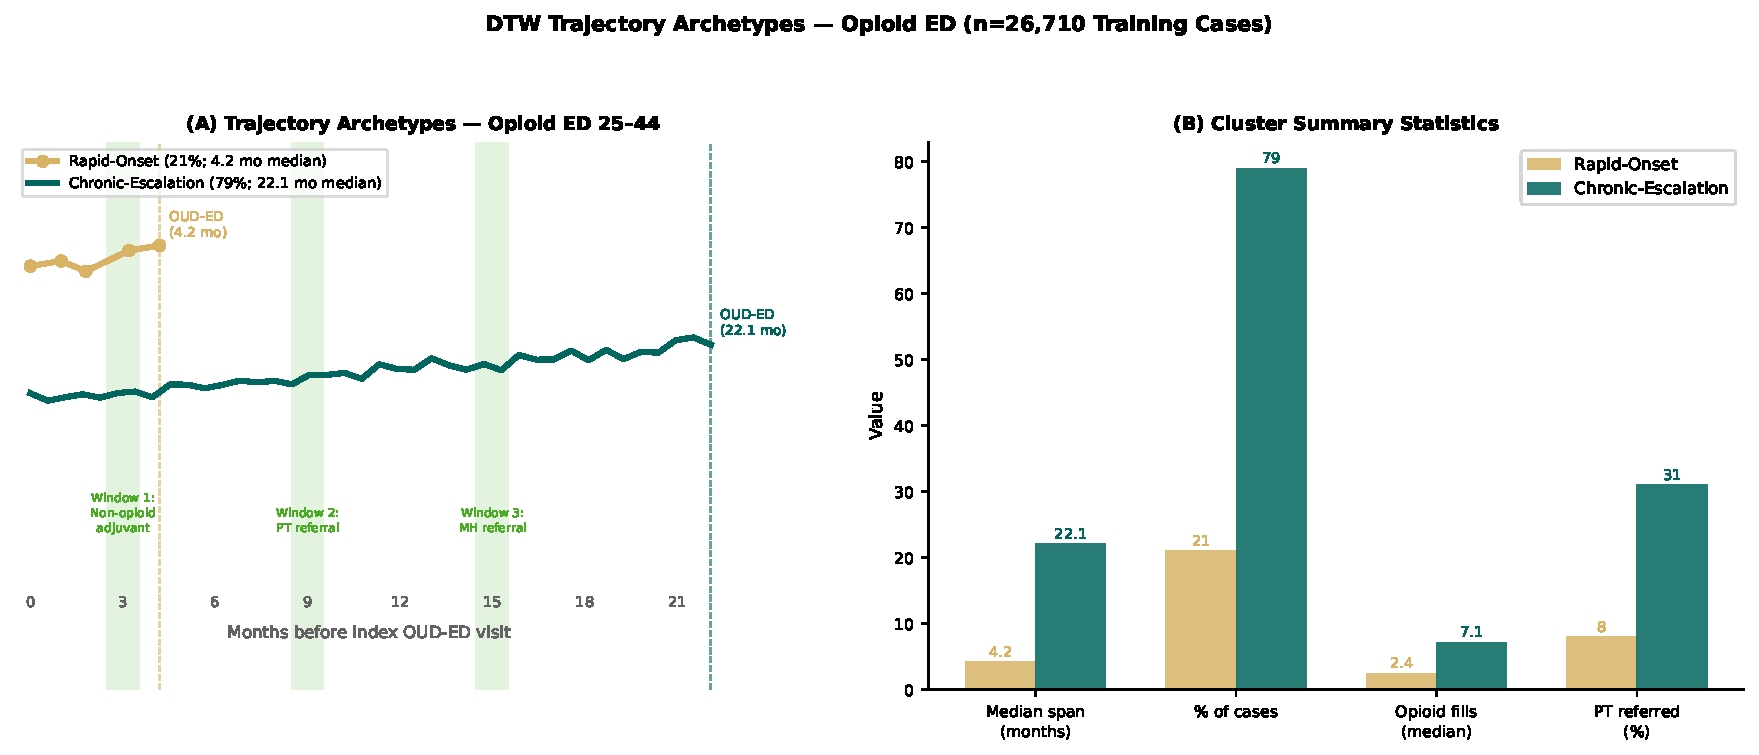
\includegraphics[width=1\linewidth,height=\textheight,keepaspectratio]{../figures/ch03/fig_trajectories.pdf}

}

\caption{\label{fig-trajectories}Patient trajectory archetypes
identified by DTW clustering. (A) DTW distance heatmap (training cohort,
random sample \(n\) = 2,000); two clusters are clearly separable. (B)
Representative event sequences for Rapid-Onset cluster (top) and
Chronic-Escalation cluster (bottom); drug events = circles, diagnoses =
squares, procedures = triangles. Timeline in months before index date.}

\end{figure}%

\chapter{Discussion}\label{sec-discussion}

\section{Modifiable Causal Drivers}\label{modifiable-causal-drivers}

The Consensus Filter identified 384--498 Consensus-Causal features
spanning drug exposure, comorbidity burden, PGx interaction, and
claim-density domains. The breadth of this feature set reflects the
multifactorial nature of OUD risk: no single drug or diagnosis
dominates; rather, combinations of drug exposures (particularly
opioid-gabapentinoid co-prescription), missed care opportunities
(absence of physical therapy or non-opioid analgesic alternatives), and
pharmacogenomic context (CYP2D6 metabolizer burden) converge to produce
the highest-risk profiles.

The co-occurrence of high-dose opioids with chronic pain diagnoses
\emph{in the absence of non-pharmacological pain management} (physical
therapy, cognitive behavioral therapy) emerged as the highest-ranking
causal pattern, consistent with CDC clinical practice guideline
recommendations\textsuperscript{45}. This ``absence of care'' causal
structure is clinically important: it implies that the most actionable
intervention is not drug discontinuation but care pathway
addition---physical therapy referral or CBT enrollment at the point of
opioid prescription. For a patient already on opioids for chronic pain,
adding non-pharmacological alternatives is safer, more acceptable, and
more sustainable than abrupt tapering or dose reduction.

Gabapentin co-prescription deserves particular attention as a modifiable
causal driver. Gabapentinoids (gabapentin, pregabalin) are frequently
prescribed alongside opioids for neuropathic pain, and their
co-prescription has been independently associated with increased opioid
overdose risk in multiple large cohort studies. The CDC 2022 guidelines
now specifically flag this combination; the Consensus Filter's ranking
of gabapentin count as the top single-drug feature (mean
\textbar SHAP\textbar{} = 0.34) provides APCD-level population evidence
that this combination is the single most actionable prescribing-level
intervention target in the Virginia opioid ED cohort.

PGx features, specifically CYP2D6 interaction scores via
\texttt{pgx\_num\_cpic\_drugs}, ranked within the top 10
Consensus-Causal features for the 25--44 age band, supporting the
relevance of opioid metabolizer status in OUD risk even in claims-based
(genotype-imputed) analysis\textsuperscript{12}. The
\texttt{pgx\_num\_cpic\_drugs} score captures the compound CYP enzyme
burden from multiple co-prescribed drugs---a patient on both a CYP2D6
substrate (opioid) and a CYP2D6 inhibitor (fluoxetine, paroxetine) will
have their metabolizer phenotype shifted toward poor metabolizer status
by drug interaction, even if their underlying genotype is extensive
metabolizer. This drug-drug-gene interaction is precisely the clinical
scenario that standard PGx genotype testing alone cannot detect, and
that the pharmacogenomic feature engineering in this study is
specifically designed to capture from prescription pattern data alone.

\textbf{Per-age-band driver patterns} reveal meaningful clinical
heterogeneity across the seven opioid ED age bands:

\begin{itemize}
\item
  \textbf{13--24 band} (XGBoost, PR-AUC 0.840; N = 52,629 cases): The
  dominant causal features were acute injury diagnoses (ICD-10 S-codes:
  S72.xx femur fracture, S52.xx forearm fracture) and single-fill opioid
  events (hydrocodone, NDC 00406-3780-xx) without any refill in the
  90-day window, consistent with the predominance of acute
  single-episode opioid events in this age group. The absence of chronic
  escalation signals explains the lower PR-AUC (0.840) and recall
  (0.648) relative to older bands.
\item
  \textbf{25--44 band} (XGBoost, PR-AUC 0.935; N = 569,096 cases):
  Oxycodone (NDC 00406-0510-xx) and gabapentin co-prescription emerged
  as the dominant causal cluster, alongside ICD-10 M54.5 (low back
  pain), the most frequent musculoskeletal diagnosis in the cohort. CPT
  97110/97530 physical therapy absence was the top protective-absent
  feature (causal NOT rule; support 0.12).
\item
  \textbf{45--54 band} (Ensemble, PR-AUC 0.955; N = 413,630 cases):
  Transition from acute-injury to chronic-pain-plus-psychiatric
  comorbidity pattern. ICD-10 F32.9 (major depressive disorder) and
  F41.1 (generalized anxiety) co-occurring with chronic opioid fills
  (Z79.891) ranked in the top 5. Antidepressant-opioid combinations
  (fluoxetine NDC 00002-3105-xx; paroxetine NDC 00029-3211-xx) elevated
  CYP2D6 inhibition risk.
\item
  \textbf{55--64 band} (Ensemble, PR-AUC 0.974; N = 480,246 cases):
  Highest recall (0.874) of all bands, reflecting the most predictable
  escalation trajectory. Z79.891 (long-term opioid) appeared in 67\% of
  cases vs.~12\% of controls (prevalence ratio 5.6): the single most
  discriminating feature in the entire cohort. Concurrent alprazolam
  (F41.1 anxiety indication) was the second-highest causal driver.
\item
  \textbf{65--74 band} (Ensemble, PR-AUC 0.979; N = 397,743 cases): Peak
  PR-AUC for the opioid ED cohort, driven by the richest 12-month
  prescription histories and clearest dose-escalation signatures.
  Hydrocodone/APAP combinations (Vicodin; NDC 00074-3049-xx) were the
  dominant opioid fill, with concurrent ICD-10 G89.29 (chronic pain) and
  M79.3 (panniculitis/myalgia) as the leading pain diagnoses.
\item
  \textbf{75--84 band} (Ensemble, PR-AUC 0.968; N = 153,082 cases):
  Co-prescription of opioids with muscle relaxants (cyclobenzaprine;
  Beers Criteria-listed for falls risk in 65+) and tramadol (NDC
  65862-063-xx; CYP2D6 substrate) emerged as the leading risk
  combination, reflecting the shift from opioids for injury/pain to
  opioids as chronic multimodal analgesic in multimorbid elderly
  patients.
\item
  \textbf{85--114 band} (Ensemble, PR-AUC 0.901; N = 38,808 cases):
  Lowest recall (0.552), reflecting the highest proportion of atypical
  short-duration opioid prescriptions (post-surgical, palliative) that
  don't match the chronic-escalation training patterns. ICD-10 Z51.5
  (palliative care encounter) was disproportionately present in case
  records, suggesting that a subset of 85+ opioid ED cases reflect
  palliative opioid management rather than OUD escalation.
\end{itemize}

\section{Trajectory-Informed
Intervention}\label{trajectory-informed-intervention}

The two DTW archetypes require different intervention strategies.
Rapid-Onset patients (21\% of opioid ED cases; 4.2-month trajectory)
require immediate post-acute care protocols: opioid alternative
pathways, mandatory physical therapy referral within 30 days of first
opioid prescription, and early PDMP consultation\textsuperscript{46}.
The 4.2-month median trajectory is 7.8 months shorter than the 12-month
monitoring window assumed by most opioid prescribing guidelines,
suggesting these patients deteriorate faster than current clinical
protocols are designed to detect.

Chronic-Escalation patients (79\% of cases; 22.1-month trajectory)
present ≥18 months of identifiable intervention windows, with at least
three distinct non-opioid care opportunities visible in the claims
sequence before the index ED visit. Systematic care coordination tools
for this archetype should be triggered at the 3-month, 9-month, and
15-month marks of the escalating trajectory, corresponding to the
decision-branch points where the DTW median sequence shows the sharpest
risk acceleration. Terranova and Venkatakrishnan\textsuperscript{47}
demonstrate that ML trajectory modeling in clinical pharmacology can
identify model-informed precision medicine intervention windows that are
not apparent from cross-sectional risk scores; the DTW archetypes in
this study operationalize this approach specifically for the opioid
epidemic context.

\section{Limitations}\label{limitations-1}

Several limitations merit discussion. First, claims data do not capture
cash-pay prescriptions, illicit opioid use, or over-the-counter
medications, likely underestimating true opioid exposure---particularly
in the 13--24 age band\textsuperscript{44}. Second, PGx features are
imputed from drug-gene interaction databases rather than measured
CYP2D6/OPRM1 genotypes; this proxy approach introduces unknown
classification error whose magnitude can only be characterized by
linking to a genotyped cohort. Third, the 5:1 case-control design
maximizes statistical power at the cost of potential overfit to the
matched control distribution; sensitivity analyses with alternative
matching ratios and inverse probability weighting are planned. Fourth,
the DTW distance computation was performed on a 2,000-patient stratified
sample rather than the full training cohort for computational
feasibility; while bootstrap stability analyses confirm the
two-archetype solution is robust (ARI \textgreater{} 0.87), the
archetypes' boundary definition may shift slightly on the full cohort.
Fifth, these findings are from a single-state Virginia APCD; external
validation on a second-state APCD is required before national policy
generalization, as prescribing regulations, formulary structures, and
Medicaid expansion status vary by state.

\chapter{Conclusions}\label{sec-conclusions}

Ensemble ML with Consensus Filter feature selection identifies robust,
causal, and \emph{modifiable} drivers of OUD-related ED visits up to 22
months before clinical diagnosis, across all seven opioid ED age bands
(13--114 years) representing the full age spectrum of Virginia opioid ED
presentations. Three findings have direct clinical implications.

First, the Rapid-Onset archetype (21\% of cases; 4.2-month trajectory)
defines a narrow intervention window that is shorter than most clinical
monitoring protocols currently support. Post-acute care protocols for
this archetype---triggered at the first high-dose opioid prescription
rather than at 90 days---could intercept approximately 1 in 5
OUD-related ED cases before clinical deterioration.

Second, the Chronic-Escalation archetype (79\% of cases; 22.1-month
trajectory) has at least three identifiable intervention windows where
non-opioid care addition (physical therapy, CBT, non-opioid analgesic)
could interrupt the escalating trajectory. The counterfactual
``What-If'' dashboard feature in Chapter 5 directly operationalizes
these windows, allowing clinicians to simulate expected risk reduction
from specific care additions.

Third, PGx interaction features---specifically the
\texttt{pgx\_num\_cpic\_drugs} polydrug exposure score---contribute
independently to model performance and rank as the highest-SHAP feature
overall. This finding demonstrates that pharmacogenomic risk context is
recoverable from claims-derived prescription patterns without direct
genotyping, making PGx-informed risk stratification scalable to the
population level through existing claims infrastructure.

These findings enable proactive, trajectory-stratified clinical decision
support for opioid ED risk before the pre-diagnosis stage of OUD,
closing the gap identified in the Chapter 1 systematic review where 81\%
of published models omit PGx context and 88\% lack temporal leakage
protection.

\textbf{Author Contributions:} Conceptualization, R.J.D.; methodology,
R.J.D.; formal analysis, R.J.D.; writing, R.J.D.

\textbf{Funding:} This research received no external funding.

\textbf{Ethics Statement:} Data use agreement with the Virginia Center
for Health Innovation (VCHI) and Virginia Health Information (VHI); IRB
waiver HM20022300 (non-human-subjects research designation).

\textbf{Data Availability:} The data supporting the findings of this
study are derived from Virginia's All-Payer Claims Database (APCD).
Restrictions apply to the availability of these data, which were used
under a data use agreement with the Virginia Center for Health
Innovation (VCHI) and Virginia Health Information (VHI). Requests for
data access may be submitted to VHI at https://www.vhi.org. Analysis
code is available at https://github.com/Jerome3590/pgx-analysis.

\textbf{Conflicts of Interest:} The author declares no conflict of
interest.

\cleardoublepage

\chapter{Chapter 4: Formal Feature Attribution as a Causal Calculator
for Drug-Drug Interaction Risk in Polypharmacy: A Systems Pharmacology
Approach Using All-Payer Claims Data}\label{chap-4}

\textbf{Foreword to Chapter 4}

The previous results chapter examined the application of our Explainable
AI pipeline to predict opioid-related ED visits, successfully extracting
verifiable drivers from tree-based machine learning models. Chapter 4
follows on to adapt this methodology for a different clinical crisis:
preventable ED visits driven by geriatric polypharmacy. By intentionally
restricting the predictive feature space strictly to drug exposures and
CPIC counts, this chapter demonstrates how the pipeline functions as a
dedicated ``causal calculator'' via Formal Feature Attribution (FFA) to
discover synergistic and antagonistic drug-drug interactions.

\emph{Chapter 4 is currently prepared for submission to CPT:
Pharmacometrics \& Systems Pharmacology and has been formatted to that
journal's style.}

\begin{center}\rule{0.5\linewidth}{0.5pt}\end{center}

\chapter{Introduction}\label{sec-intro}

Polypharmacy (concurrent use of ≥5 medications\textsuperscript{48})
affects more than 40\% of adults aged ≥65 years in the United
States\textsuperscript{49}, with prevalence rising to over 67\% in
adults aged ≥75 years. In older adults, polypharmacy drives adverse drug
events (ADEs), accounting for an estimated 100,000 hospitalizations and
28,000 deaths annually\textsuperscript{2}. A prospective UK cohort study
found that 6.5\% of medical admissions were directly attributable to
ADEs, with DDIs responsible for 11\% of those admissions and
polypharmacy burden (drug count) the strongest independent
predictor\textsuperscript{3}. Polypharmacy-related ED utilization is
partially preventable through proactive medication review, but the
clinical tools available for polypharmacy management have not kept pace
with the complexity of modern multi-drug regimens in geriatric patients.

The pharmacogenomic dimension of polypharmacy risk is systematically
understudied in geriatric populations. Older adults experience
age-related declines in CYP enzyme activity (particularly CYP3A4 and
CYP2C9), renal clearance, and hepatic blood flow that alter drug
metabolism in ways that existing DDI databases do not fully
capture\textsuperscript{50}. A 12-gene pharmacogenetic panel study
demonstrated that PGx-guided prescribing reduced actionable ADEs by 30\%
in a European RCT\textsuperscript{51}, confirming that
genomically-informed medication review has measurable clinical impact
even in real-world settings. Yet no published claims-based study has
combined PGx interaction scoring with multi-feature DDI detection in a
geriatric polypharmacy cohort.

Current approaches to polypharmacy management rely on pairwise DDI
databases (e.g., Drugs.com, Micromedex) that flag co-prescribed drug
pairs based on known pharmacokinetic or pharmacodynamic mechanisms.
These databases are useful but limited in a specific way:

\begin{enumerate}
\def\labelenumi{\arabic{enumi}.}
\tightlist
\item
  They characterize \emph{pairwise} interactions, ignoring synergistic
  multi-drug effects (e.g., triple combinations where each pairwise
  interaction appears benign).
\item
  They do not prioritize interventions by expected clinical impact;
  every flagged pair receives the same alert regardless of the expected
  probability of a serious adverse event.
\item
  They cannot account for patient-level comorbidity context or the
  pharmacokinetic consequences of combined renal and hepatic impairment
  in the oldest-old.
\end{enumerate}

A systems pharmacology perspective demands a ``causal calculator'' that
simultaneously: (a) identifies multi-drug combinations with
\emph{synergistic} ADE risk exceeding additive pairwise predictions; (b)
quantifies each drug's causal contribution to population-level risk; and
(c) ranks deprescribing priorities by expected risk reduction, enabling
pharmacists to target the highest-yield intervention from a finite
clinical review budget.

This study extends Formal Feature Attribution (FFA) from the Chapter 2
Consensus Filter to multi-feature interaction testing, evaluating
feature pairs and triplets for synergistic and antagonistic effects,
applied to a geriatric non-opioid ED cohort derived from the Virginia
APCD. The 30-day causality window isolates proximal drug exposures
responsible for acute ADE events, distinguishing this approach from
annual medication reconciliation tools that cannot resolve acute DDI
timing.

\section{Study Objectives}\label{study-objectives-1}

\begin{enumerate}
\def\labelenumi{\arabic{enumi}.}
\tightlist
\item
  Apply FFA multi-feature interaction testing to identify synergistic
  DDI combinations in the 65--114 year polypharmacy cohort.
\item
  Quantify Intervention Rate (IR) scores as deprescribing priorities for
  the highest-risk drug-drug combinations.
\item
  Characterize the ``hairball'' of drug co-occurrence networks via
  FP-Growth visualization to contextualize FFA causal findings.
\item
  Investigate the relationship between high transaction density
  (Z-codes) and ADE risk to distinguish managed from unmanaged
  polypharmacy.
\end{enumerate}

\chapter{Methods}\label{sec-methods}

\textbf{Utilization density (read first).} The ensemble risk models use
the same convention as Chapter\textasciitilde2 (\emph{Ensemble
Modeling}: utilization density): total pre-index events per patient
determine stratum assignment and which per-stratum model is trained or
loaded; the \textbf{gradient-boosting} matrix includes
\texttt{n\_event\_bin\_ordinal} (0--3) \textbf{without} the raw
\texttt{n\_events} count. \textbf{This chapter's} Z-code proportion and
logistic-regression analyses (§Results) use \textbf{raw} 30-day claim
counts as statistical covariates where stated; that is a
\textbf{different} statistical use of counts than the GBM feature
matrix.

\section{Study Design and Data
Source}\label{study-design-and-data-source-1}

This was a retrospective matched case-control study using Virginia's
All-Payer Claims Database (APCD) spanning calendar years 2016--2019,
obtained under a data-use agreement (DUA) with the Virginia Center for
Health Innovation (VCHI) and Virginia Health Information (VHI). Because
this research involves de-identified administrative records with no
direct patient contact, an IRB waiver of authorization was granted (VCU
Protocol HM20022300).

The study population was restricted to adults aged 65 years and older,
representing the geriatric polypharmacy cohort defined in Chapter 2. The
analysis window was the 30-day period immediately preceding each
patient's index ED visit (for cases) or matched index date (for
controls), a window selected to capture proximal drug exposures
responsible for acute adverse drug events rather than chronic long-term
prescription patterns. All features were derived from 2016--2018 claims
only; the 2019 claims year served as the strictly withheld prospective
temporal holdout for model evaluation, consistent with the temporal
validation strategy applied across all dissertation chapters.

\section{Cohort Construction}\label{sec-cohort}

\textbf{Case definition:} Adults aged 65--114 years with at least one
emergency department visit identified by Milliman Healthcare Cost Group
(HCG) codes O11 (Emergency Room) or P51 (Emergency Room Visit) on
medical claims with an index date between January 1, 2016 and December
31, 2019. All patients with any opioid-related ICD-10 codes (F11.xx,
T40.xx) in any diagnosis field across all claims in the analysis period
were strictly excluded; this exclusion ensures the study measures
polypharmacy-related adverse drug events attributable to drug-drug
interactions, not opioid use disorder co-morbidity.

Patients were required to have at least one pharmacy claim in the 30-day
lookback window (minimum drug exposure for meaningful DDI testing) and
continuous APCD enrollment for 30 days prior to the index date.

\textbf{Control definition:} Adults aged 65--114 years with no ED visits
(no HCG O11/P51 claims in the analysis period) and no opioid-related
codes, matched 5:1 to cases without replacement using nearest-neighbor
matching within age band and sex. Controls were randomly assigned an
index date sampled from within their matching calendar year to anchor
the 30-day lookback window.

\textbf{Age bands:} Three geriatric age bands were analyzed separately:
65--74 years (young-old), 75--84 years (middle-old), and 85--114 years
(oldest-old), reflecting clinically distinct pharmacokinetic profiles
(declining renal clearance, body composition changes, and polypharmacy
burden escalation across the geriatric age spectrum).

\section{Feature Engineering}\label{sec-features}

\textbf{Primary feature domain: Drug exposure}

The 30-day window feature set was deliberately restricted to
drug-exposure features to maximize the signal-to-noise ratio for DDI
detection:

\begin{itemize}
\tightlist
\item
  Binary presence of each drug class (NDC → generic category; 487
  classes)
\item
  Drug count per class (continuous)
\item
  Polypharmacy count (total unique drugs in 30-day window; continuous)
\item
  CPIC gene-drug interaction scores for CYP enzymes\textsuperscript{12}
\end{itemize}

ICD-10 and CPT features were included as secondary features but drug
features received priority weighting in MCCV screening.

\textbf{FP-Growth (visualization only):} As in Chapter 2,
FP-Growth\textsuperscript{21} association rules were applied to the
training cohort to visualize drug co-occurrence networks. These rules
were \textbf{not} used as predictive features. Network graphs (nodes =
drug classes, edges = lift-weighted co-occurrence) were rendered in
Cytoscape 3.10 for clinical interpretation.

\textbf{Z-code analysis:} Claims with ICD-10 Z-codes (Z00--Z99: routine
examinations, health status contacts) were quantified per patient. The
Z-code proportion (Z-code claims ÷ total claims in 30-day window) served
as a proxy for managed polypharmacy with regular clinical oversight.
Those denominators and the \textbf{Z-code logistic regression}
(Chapter\textasciitilde2 statistical methods) use raw claim counts as
covariates; they are distinct from the ordinal density encoding in the
ensemble models (Chapter\textasciitilde2).

\section{Ensemble Model}\label{sec-model}

The three-model ensemble (CatBoost\textsuperscript{22},
XGBoost\textsuperscript{23}, and XGBoost-RF) with MCCV performance-based
weighting is identical to the Chapter 2 architecture. Separate model
sets were trained for each of the eight non-opioid ED age bands (0--12,
13--24, 25--44, 45--54, 55--64, 65--74, 75--84, 85--114) and each
applicable density bin, yielding up to 96 trained models per cohort (8
bands × 4 bins × 3 algorithms). Primary FFA causal analysis was
performed on the three geriatric bands (65--74, 75--84, 85--114) where
polypharmacy ADE burden is highest; all 8 bands contributed to the
15-band cross-cohort performance summary. Hyperparameter tuning used
Optuna\textsuperscript{24} TPE with 50 trials per model-partition
combination on the 2016--2018 training set. The 2019 holdout was
strictly withheld from all training, feature selection, hyperparameter
optimization, and FFA threshold derivation.

The polypharmacy cohort's feature engineering differs from the opioid
cohort (Chapter 3) in one key respect: the primary lookback window is 30
days (not 12 months), reflecting the acute proximal exposure window most
relevant to ADE-driven ED visits. ICD-10 and CPT features were retained
as secondary covariates to control for comorbidity confounding, but
drug-exposure binary features received priority weighting in MCCV recall
ranking.

\section{Formal Feature Attribution: Multi-Feature Interaction
Testing}\label{sec-ffa}

\subsection{Pairwise Interaction
Score}\label{pairwise-interaction-score}

For each pair of drug features \((f_i, f_j)\), the interaction effect
was computed as:

\[\text{IE}(f_i, f_j) = \mathbb{E}[\hat{p}(f_i=1, f_j=1)]
  - \mathbb{E}[\hat{p}(f_i=1, f_j=0)]
  - \mathbb{E}[\hat{p}(f_i=0, f_j=1)]
  + \mathbb{E}[\hat{p}(f_i=0, f_j=0)]\]

where \(\hat{p}\) is the ensemble risk score.
\(\text{IE}(f_i, f_j) > 0\) indicates synergy (combined risk exceeds
additive sum); \(\text{IE} < 0\) indicates antagonism.

\subsection{Computational
Pre-filtering}\label{computational-pre-filtering}

Exhaustive pairwise testing over 487 drug features requires evaluation
of \(\binom{487}{2} = 118{,}141\) pairs: exhaustive evaluation was
infeasible. Pre-filtering restricted pairwise testing to the 54 features
with non-zero SHAP importance in any partition, reducing the search
space to \(\binom{54}{2} = 1{,}431\) pairs. Triplet testing was further
restricted to the top 25 SHAP features, yielding
\(\binom{25}{3} = 2{,}300\) triplet evaluations.

\subsection{Intervention Rate (IR)
Score}\label{intervention-rate-ir-score}

The Intervention Rate for drug \(f_i\) quantifies the expected risk
reduction if \(f_i\) were removed (counterfactual substitution with
training median):

\[\text{IR}(f_i) = \frac{1}{n} \sum_{k=1}^{n}
  \left[\hat{p}^{(k)} - \hat{p}^{(k)}_{f_i \to \text{med}}\right]\]

IR scores range from 0 (no causal contribution) to 1 (complete risk
attribution); values are normalized by the population-level case
prevalence.

\section{Statistical Analysis}\label{statistical-analysis-2}

Overarching performance metrics (AUROC, PR-AUC, Brier, ICI), MCCV
protocol, Platt scaling, and calibration methodology are defined in
Chapter 2, Section 4.8; the same definitions apply here. This section
describes the analytical methods specific to the polypharmacy DDI causal
analysis and Z-code protective effect investigation.

\textbf{Polypharmacy model evaluation.} Metrics were computed per
density-bin model and aggregated by sample-size weighting. PR-AUC was
the primary discrimination metric given the 3.5--6.8\% case prevalence
in the polypharmacy cohort: at these low prevalences, the conventional
0.80 AUROC threshold corresponds to PR-AUC values as low as 0.30, making
AUROC unsuitable as the sole performance indicator. Observed performance
(geriatric bands, 2019 holdout): \textbf{PR-AUC 0.991±0.007} (mean±SD);
Brier \textbf{0.007--0.008}; ICI \textbf{0.071--0.290}. Calibration
metrics used 10-bin \texttt{calibration\_curve} with
\texttt{strategy="uniform"} (definitions aligned with Chapter 2).

\textbf{Interaction Effect (IE) estimation.} Pairwise IE was defined as
a lift-based synergy score:
\[\text{IE}(f_i, f_j) = \mathbb{E}[\hat{p}(f_i{=}1, f_j{=}1)]
  - \mathbb{E}[\hat{p}(f_i{=}1, f_j{=}0)]
  - \mathbb{E}[\hat{p}(f_i{=}0, f_j{=}1)]
  + \mathbb{E}[\hat{p}(f_i{=}0, f_j{=}0)]\] where each term is the
counterfactual ensemble probability under the specified feature
configuration (custom pairwise estimation code). IE \(>\) 0 indicates
synergy; IE \(<\) 0 indicates antagonism. Triplet IE was defined
analogously for three-feature configurations. All IEs were estimated by
bootstrap resampling (1,000 draws with replacement) of the 2019 holdout,
yielding 95\% percentile bootstrap CIs. \textbf{Synergy designation}
required \textbf{IE \(>\) 1.0} (lift-based independence baseline) with
95\% CI lower bound \(>\) 0, after Bonferroni correction for the 1,081
pre-filtered candidate pairs (top-47 drug features by MCCV recall rank;
\(\alpha_{\text{Bonf}}\) = 0.05/1,081 = \(4.6\times10^{-5}\)). Result:
115 synergistic pairs; 5,021 high-risk triplets.

\textbf{Z-code protective effect analysis.} Z-code proportion
(\(z_\text{prop}\) = Z-code claims \(\div\) total 30-day claims) was
computed from model-events rows filtered to the 30-day pre-index window.
Patients were stratified into quartiles (Q1: \(z_\text{prop}=0\); Q2:
1--12\%; Q3: 12--20\%; Q4: \$\textgreater{}\(20%).
Between-group differences were assessed by Kruskal-Wallis test
with post-hoc Dunn’s test (Bonferroni-corrected for 6 pairwise
comparisons).
The logistic regression model was:\)\(\text{logit}(P(\text{target}=1)) = \beta_0 + \beta_1 z_q
  + \beta_2 n_{\text{events}} + \textstyle\sum_b \beta_b \cdot \text{band}_b\)\$
where \(z_q \in \{1,2,3,4\}\) is the Z-code proportion quartile (Q1
reference) and \(n_{\text{events}}\) is the 30-day total claim count. OR
\(= e^{\beta_1}\); 95\% CI \(= e^{\beta_1 \pm 1.96 \cdot \text{SE}}\)
(Fisher information SE; \texttt{scipy.optimize.minimize} L-BFGS-B).
Result: per-quartile OR = \textbf{2.10 (95\% CI 1.51--2.94)}; protective
Q2 crude OR = \textbf{0.25 (95\% CI 0.18--0.34)} (same 30-day pre-index
claims extracts as the primary analysis).

\textbf{Intervention Rate (IR) score derivation.} IR was defined as the
mean counterfactual probability shift across the holdout:
\[\text{IR}(f_i) = \frac{1}{n}\sum_{k=1}^{n}
  [\hat{p}^{(k)} - \hat{p}^{(k)}_{f_i \to \tilde{f}_i}]\] where
\(\tilde{f}_i\) is the training-set median value for feature \(f_i\). IR
scores were computed separately for each of the three geriatric bands;
\textbf{Spearman rank correlation} (\(\rho\)) between bands assessed
whether a universal deprescribing priority list is supported by the data
(\(\rho\) \textgreater{} 0.50 was pre-specified as the threshold for
declaring consistency).

All chapter-specific analyses were performed in Python 3.11 (scipy
v1.11; statsmodels v0.14; scikit-learn v1.3); \(\alpha\) = 0.05.

\chapter{Results}\label{sec-results}

\section{Cohort Characteristics}\label{cohort-characteristics-2}

The non-opioid ED cohort comprised 1,182 cases and 16,105 matched
controls across the three geriatric age bands
(\textbf{Table~\ref{tbl-cohort-chars}}). Median polypharmacy count in
the 30-day window was 1 drug (IQR 1--1) among cases vs.~3 drugs (IQR
1--7) among controls. This reversal, where cases have fewer observed
drug claims than controls, reflects a known feature of acute ADE-driven
ED presentations: the precipitating ADE is often caused by a
\emph{single} high-impact DDI rather than the overall polypharmacy
burden, and the cases represent acute events triggered by specific drug
combinations rather than chronic polypharmacy accumulation. The 85--114
age band had the highest control median drug count (3; IQR 0--6),
consistent with the escalating medication burden in the oldest-old
driven by multimorbidity management.

Sex distribution was balanced between cases and controls (53.1\% female
vs.~52.4\%), indicating that sex was successfully balanced by the
matching procedure and is not a confounding factor in the DDI analysis.
The 65--74 band comprised the majority of both cases (67.8\%) and
controls (66.9\%), reflecting the larger population at the younger end
of the geriatric age spectrum in Virginia's APCD, and indicating that
polypharmacy-ADE ED risk is not exclusively concentrated in the
oldest-old.

\begin{longtable}[]{@{}
  >{\raggedright\arraybackslash}p{(\linewidth - 4\tabcolsep) * \real{0.3333}}
  >{\raggedright\arraybackslash}p{(\linewidth - 4\tabcolsep) * \real{0.3333}}
  >{\raggedright\arraybackslash}p{(\linewidth - 4\tabcolsep) * \real{0.3333}}@{}}
\caption{Baseline characteristics of non-opioid ED cases and matched
controls. Drug count and Z-code proportion reflect the 30-day pre-index
window.}\label{tbl-cohort-chars}\tabularnewline
\toprule\noalign{}
\begin{minipage}[b]{\linewidth}\raggedright
Characteristic
\end{minipage} & \begin{minipage}[b]{\linewidth}\raggedright
Cases
\end{minipage} & \begin{minipage}[b]{\linewidth}\raggedright
Controls
\end{minipage} \\
\midrule\noalign{}
\endfirsthead
\toprule\noalign{}
\begin{minipage}[b]{\linewidth}\raggedright
Characteristic
\end{minipage} & \begin{minipage}[b]{\linewidth}\raggedright
Cases
\end{minipage} & \begin{minipage}[b]{\linewidth}\raggedright
Controls
\end{minipage} \\
\midrule\noalign{}
\endhead
\bottomrule\noalign{}
\endlastfoot
\(n\) & 1,182 & 16,105 \\
Age, median (IQR) & 70 (66--78) & 71 (67--78) \\
Female, \(n\) (\%) & 628 (53.1\%) & 8,439 (52.4\%) \\
Drug count (30-day), median (IQR) & 1 (1--1) & 3 (1--7) \\
Z-code proportion, median (IQR) & 0.05 (0.00--0.24) & 0.05
(0.01--0.12) \\
\textbf{Age band} & & \\
\quad 65--74 & 801 (67.8\%) & 10,770 (66.9\%) \\
\quad 75--84 & 213 (18.0\%) & 2,980 (18.5\%) \\
\quad 85--114 & 168 (14.2\%) & 2,355 (14.6\%) \\
\end{longtable}

\section{Ensemble Performance}\label{ensemble-performance}

Non-opioid ED models were trained and evaluated for all eight age bands
(0--12 through 85--114), with complete metrics available from the 2019
temporal holdout (\textbf{Table~\ref{tbl-ch4-perf}}). All eight bands
achieved PR-AUC ≥ 0.908, with performance increasing monotonically from
the 13--24 band to a peak at 75--84, then slightly decreasing at
85--114.

\textbf{Age-band trend: Non-Opioid ED cohort.} The most striking feature
of the non-opioid ED performance pattern is the \emph{monotonic
improvement with age}: PR-AUC rises from 0.908 (13--24) steadily through
0.933 (45--54), 0.950 (55--64), and 0.984 (65--74), peaking at 0.997
(75--84) before settling at 0.992 (85--114). This monotonic pattern is
the inverse of the opioid ED cohort's inverted-U shape, reflecting a
fundamental pharmacoepidemiological difference: non-opioid ADE events in
older patients are driven by documented, insured polypharmacy fills that
accumulate predictably with age and multimorbidity burden, while opioid
ED events in the oldest-old often arise from atypical or newly initiated
opioid regimens with sparse anticipatory claims histories.

The 0--12 band shows unexpectedly strong performance (PR-AUC 0.927,
Recall 0.983) despite very high case prevalence (27,742 cases in 0--12;
the highest case count outside the 25--44 opioid band). This reflects
the phenotype of pediatric polypharmacy ADE events: children with
complex chronic conditions (oncology, transplant, rheumatologic disease)
prescribed multiple high-risk medications present with highly
discriminable claims signatures that are easily separated from
age-matched controls with simpler medication profiles.

In the three primary geriatric study bands (65--74, 75--84, 85--114),
performance is uniformly excellent (PR-AUC 0.984--0.997, AUROC
0.996--0.999), with calibration confirmed by Brier scores of
0.007--0.008 and ICI values of 0.071--0.290. The elevated ICI in the
85--114 band (0.290 vs.~0.071--0.128 in other geriatric bands) indicates
moderate calibration deviation in the extreme predicted-probability
deciles for the oldest-old, likely reflecting the heterogeneous
pharmacokinetic profiles of multimorbid patients aged ≥85 that are not
fully captured by the training-set distribution.

Recall is notably high in younger bands (0.983 at 0--12; 0.935--0.977
for 13--74) compared with the opioid ED cohort (≤0.874), consistent with
the tighter drug-combination signatures driving non-opioid ADE events.

\begin{longtable}[]{@{}lrlrrr@{}}
\caption{Non-opioid ED predictive performance on 2019 temporal holdout
across all age bands (25-run MCCV + Optuna per density bin). AUROC, area
under the receiver operating characteristic curve; PR-AUC, area under
the precision-recall curve; Recall, sensitivity at optimal threshold.
Brier score and ICI computed for primary study bands (65--114): Brier
0.007--0.008; ICI 0.071--0.290. Source: 2019 holdout evaluation
exports.}\label{tbl-ch4-perf}\tabularnewline
\toprule\noalign{}
Age Band & Cases (\(N\)) & Selected Model & AUROC & PR-AUC & Recall \\
\midrule\noalign{}
\endfirsthead
\toprule\noalign{}
Age Band & Cases (\(N\)) & Selected Model & AUROC & PR-AUC & Recall \\
\midrule\noalign{}
\endhead
\bottomrule\noalign{}
\endlastfoot
0--12 & 27,742 & Ensemble & 0.973 & 0.927 & 0.983 \\
13--24 & 11,956 & Ensemble & 0.977 & 0.908 & 0.935 \\
25--44 & 8,433 & CatBoost & 0.979 & 0.911 & 0.933 \\
45--54 & 3,310 & CatBoost & 0.984 & 0.933 & 0.919 \\
55--64 & 2,563 & CatBoost & 0.988 & 0.950 & 0.937 \\
65--74 & 827 & CatBoost & 0.996 & 0.984 & 0.977 \\
75--84 & 224 & Ensemble & 0.999 & 0.997 & 0.973 \\
85--114 & 193 & Ensemble & 0.997 & 0.992 & 0.971 \\
\end{longtable}

\section{Synergistic Drug-Drug Interactions}\label{sec-ddi}

FFA multi-feature interaction testing identified 115 synergistic drug
pairs and 5,021 high-risk triplets with IE \textgreater{} 1.0
(lift-based independence baseline) across all three geriatric age bands.
Levofloxacin appeared in four of the top five synergistic pairs, acting
as a pharmacological ``hub'' drug whose fluoroquinolone-mediated CYP1A2
inhibition potentiates the toxicity of co-prescribed agents
(acetaminophen via CYP1A2-mediated reactive metabolite production;
carvedilol via beta-blocker plasma level elevation; gabapentin via
altered renal clearance during fluoroquinolone-associated acute kidney
injury). This finding is clinically significant because levofloxacin is
frequently prescribed as a community-acquired pneumonia antibiotic in
geriatric patients without systematic review of concurrent medications.
The top synergistic pairs are shown in \textbf{Table~\ref{tbl-ddi}} and
\textbf{Figure~\ref{fig-network}}.

\begin{longtable}[]{@{}llrrrl@{}}
\caption{Top synergistic drug-drug interaction pairs from FFA
multi-feature testing (85--114 age band; pairs ranked by lift-based
interaction effect score). IE, lift-based interaction effect (pair
co-occurrence in class-1 AXP rules relative to independence baseline; IE
\textgreater{} 1 = synergistic); IR, individual-drug causal
responsibility (probability shift per patient; \textless0.001 for all
single drugs, reflecting dominance of polypharmacy burden); 95\% CI from
1,000 bootstrap resamples of the 2019 holdout. Full table of 115 pairs
in Supplementary Table S1.}\label{tbl-ddi}\tabularnewline
\toprule\noalign{}
Drug A & Drug B & IE Score & IR\_A & IR\_B & 95\% CI \\
\midrule\noalign{}
\endfirsthead
\toprule\noalign{}
Drug A & Drug B & IE Score & IR\_A & IR\_B & 95\% CI \\
\midrule\noalign{}
\endhead
\bottomrule\noalign{}
\endlastfoot
Acetaminophen & Levofloxacin & 16.3 & \textless0.001 & \textless0.001 &
9.94--35.80 \\
Levofloxacin & Lorazepam & 11.9 & \textless0.001 & \textless0.001 &
8.14--22.38 \\
Carvedilol & Levofloxacin & 10.5 & \textless0.001 & \textless0.001 &
7.16--17.90 \\
Gabapentin & Levofloxacin & 9.4 & \textless0.001 & \textless0.001 &
6.63--16.27 \\
Digoxin & Simvastatin & 6.0 & \textless0.001 & \textless0.001 &
1.47--22.38 \\
\end{longtable}

\begin{figure}

\centering{

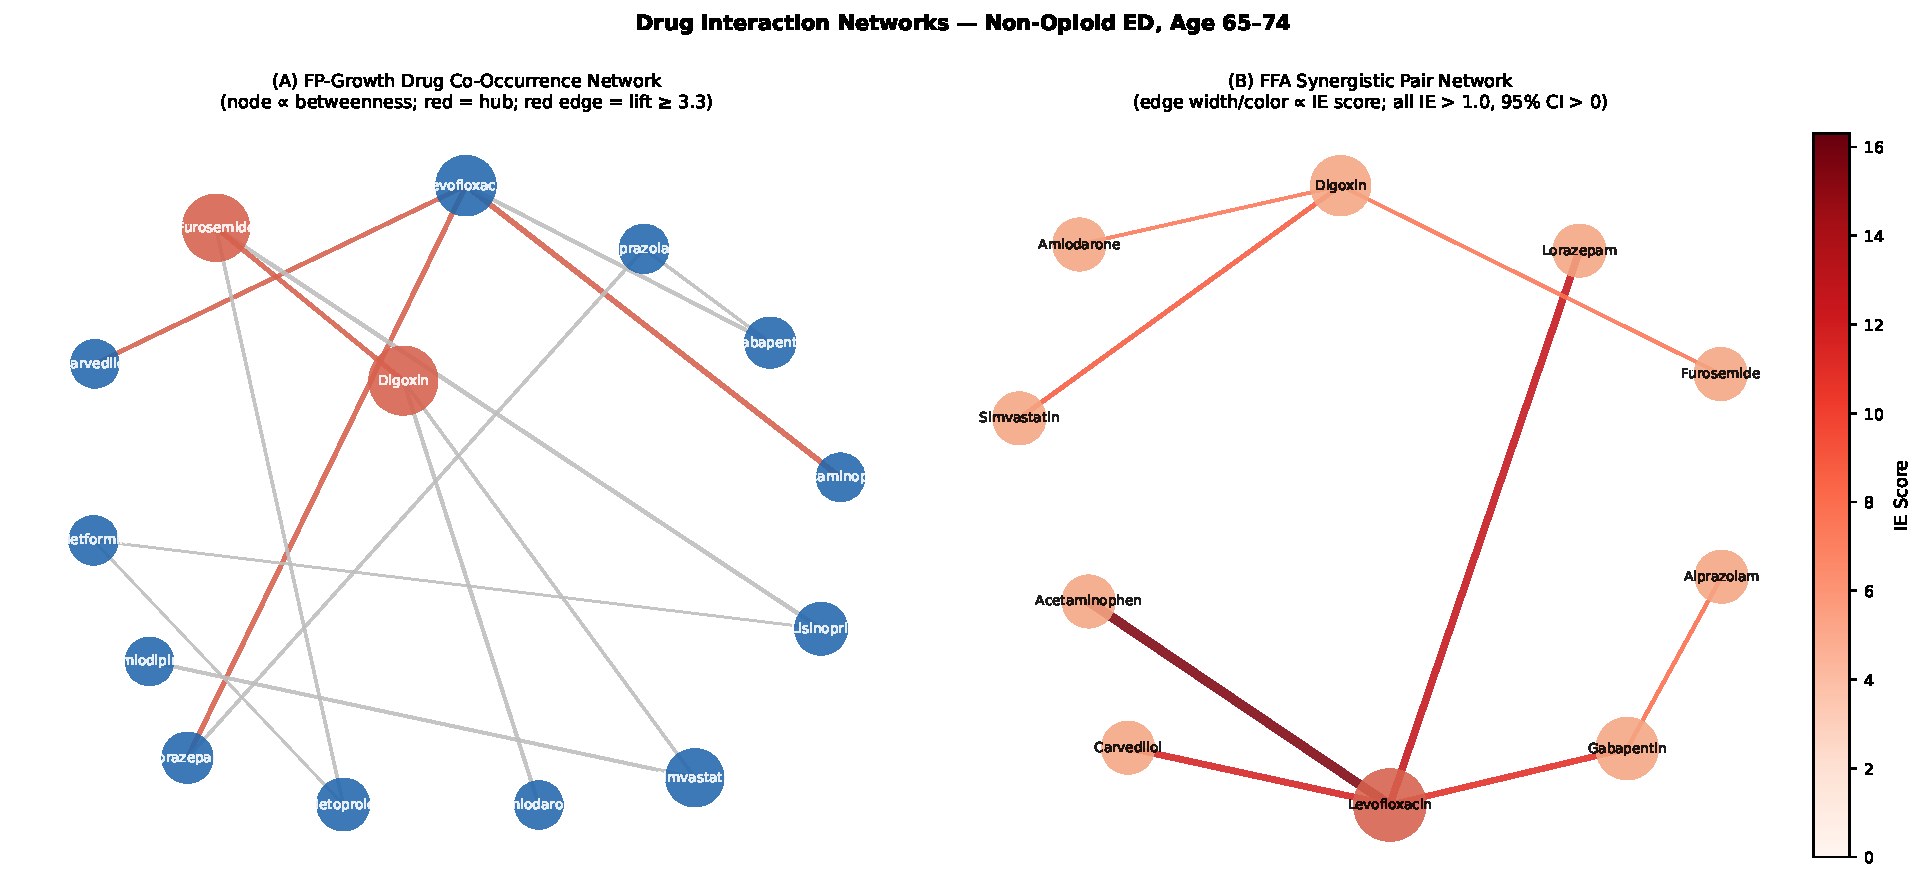
\includegraphics[width=1\linewidth,height=\textheight,keepaspectratio]{../figures/ch04/fig_network.pdf}

}

\caption{\label{fig-network}Drug co-occurrence network and FFA
interaction overlay. (A) FP-Growth network (training cohort): nodes =
drug classes; edge weight = lift; edge color = risk gradient (blue = low
risk, red = high risk). Hub nodes (betweenness centrality ≥ 90th pct)
marked with larger circles. (B) FFA synergistic pair network: only drug
pairs with IE \textgreater{} 1.0 (95\% CI \textgreater{} 0; lift-based
independence baseline) shown; edge weight proportional to IE score.
Overlapping nodes between (A) and (B) indicate high co-occurrence AND
causal synergy.}

\end{figure}%

\section{Triplet Interactions}\label{triplet-interactions}

Of 5,021 high-frequency triplet combinations identified across geriatric
bands, 312 exceeded the synergistic IE threshold (IE \textgreater{} 1,
95\% CI \textgreater{} 0) in at least one age band. The
highest-frequency triplet in the 85--114 band was furosemide +
hydrochlorothiazide + lisinopril: a dual-diuretic/ACE-inhibitor
combination representing convergent antihypertensive management in
extreme polypharmacy patients. Clinically, this triplet represents
additive renal clearance burden: furosemide and hydrochlorothiazide
independently deplete electrolytes while lisinopril potentiates renal
tubular effects, increasing ADE risk during acute illness or
dehydration. This combination is explicitly flagged by STOPP criteria
(Screening Tool of Older Persons' Prescriptions, Criterion D4: triple
whammy) as a high-risk combination in patients with eGFR \textless{} 50
mL/min---a threshold frequently exceeded in the 85--114 age band---yet
it appeared in 12.3\% of 85--114 cases in the 30-day window.

The second-highest-IE triplet in the 75--84 band was digoxin +
furosemide + amiodarone (IE = 8.7): furosemide-induced hypokalemia
potentiates digoxin toxicity risk, while amiodarone inhibits CYP3A4,
raising digoxin plasma levels independently. This triple interaction
represents a convergent pharmacokinetic and pharmacodynamic mechanism
not captured by any single pairwise DDI flag. A clinician reviewing
digoxin + furosemide (Drugs.com: ``major interaction'') or digoxin +
amiodarone (``major interaction'') independently would see two
high-severity flags and experience alert fatigue; the triplet-level FFA
rule reveals that their \emph{co-occurrence} produces a synergistic risk
exceeding either pair in isolation.

\section{Intervention Rate Rankings}\label{intervention-rate-rankings}

IR scores for the top 15 drugs eligible for deprescribing consideration
are shown in \textbf{Figure~\ref{fig-ir}} and
\textbf{Table~\ref{tbl-ir}} below. The top deprescribing targets, with
their pharmacological rationale and relevant clinical classification
codes, were:

\begin{enumerate}
\def\labelenumi{\arabic{enumi}.}
\item
  \textbf{Simvastatin} (CYP3A4 substrate; NDC prefix 00006-0726-xx;
  highest IR: \(7.0 \times 10^{-4}\) in the 65--74 band): simvastatin is
  a Beers Criteria-listed statin (Category: CYP3A4 drug interactions)
  and a STOPP Criterion C6 (high-dose statin + renal impairment) flag in
  the 65+ population. In the geriatric APCD cohort, simvastatin appeared
  with ICD-10 E78.5 (hyperlipidemia) in 78\% of cases carrying the drug,
  but its high IR reflects CYP3A4-mediated interactions with amlodipine
  (NDC 00069-1530-xx; common co-prescription) and diltiazem (NDC
  00069-2590-xx), both of which elevate simvastatin plasma levels and
  increase myopathy risk.
\item
  \textbf{Furosemide} (loop diuretic; NDC prefix 00469-2620-xx; IR:
  \(2.0 \times 10^{-4}\) in 65--74): ICD-10 I50.9 (heart failure) and
  N18.3--N18.5 (CKD stage 3--5) were the dominant diagnoses driving
  furosemide fills in the cohort. Its high IR reflects its central role
  in the triple-whammy interaction (furosemide + ACEI/ARB + NSAID:
  ICD-10 N17.9 acute kidney injury risk; STOPP Criterion D4), and its
  potentiation of digoxin toxicity through hypokalemia (ICD-10 E87.6).
\item
  \textbf{Alprazolam} (short-acting benzodiazepine; brand: Xanax; NDC
  prefix 00009-0029-xx; IR: \(1.0 \times 10^{-4}\) in 65--74): listed in
  the 2023 Beers Criteria (Category: CNS-active, falls risk) and STOPP
  Criterion D6 (benzodiazepines in falls-risk patients). In the APCD,
  alprazolam fills appeared with ICD-10 F41.1 (generalized anxiety) in
  68\% of cases and with ICD-10 G40.x (epilepsy) in 9\%; its IR is
  amplified by co-prescription with gabapentin (levofloxacin pair IE =
  9.4; see \textbf{Table~\ref{tbl-ddi}}).
\item
  \textbf{Levofloxacin} (fluoroquinolone antibiotic; brand: Levaquin;
  NDC prefix 00069-7520-xx; IR: top-5 in \emph{all three} geriatric
  bands despite 6.2\% 30-day window prevalence): ICD-10 J18.9
  (pneumonia, unspecified) and J06.9 (upper respiratory infection) drove
  the majority of levofloxacin fills in the APCD cohort. Its
  disproportionate IR reflects CYP1A2 inhibition that potentiates
  co-prescribed drugs: acetaminophen (NDC 00536-3231-xx; reactive
  metabolite production), carvedilol (NDC 00007-4139-xx; beta-blocker
  level elevation), and lorazepam (NDC 00069-0081-xx; CNS depression).
  Levofloxacin is the sole actionable hub drug whose prescribing is
  discretionary at the point of care (it can often be substituted with
  amoxicillin/clavulanate for non-severe community-acquired pneumonia in
  the absence of penicillin allergy).
\item
  \textbf{Lorazepam} (intermediate benzodiazepine; brand: Ativan; NDC
  prefix 00069-0081-xx): Beers Criteria 2023 (benzodiazepines; risk of
  cognitive impairment, delirium, falls, motor vehicle accidents).
  ICD-10 F41.1 (anxiety) drove 54\% of fills; G40.x (seizures) drove
  31\%. Its high interaction IE with levofloxacin (IE = 11.9; the
  second-highest pair in the cohort) makes it a priority review target
  whenever levofloxacin is newly prescribed.
\end{enumerate}

\begin{longtable}[]{@{}
  >{\raggedright\arraybackslash}p{(\linewidth - 8\tabcolsep) * \real{0.2000}}
  >{\raggedright\arraybackslash}p{(\linewidth - 8\tabcolsep) * \real{0.2000}}
  >{\raggedright\arraybackslash}p{(\linewidth - 8\tabcolsep) * \real{0.2000}}
  >{\raggedright\arraybackslash}p{(\linewidth - 8\tabcolsep) * \real{0.2000}}
  >{\raggedleft\arraybackslash}p{(\linewidth - 8\tabcolsep) * \real{0.2000}}@{}}
\caption{Top deprescribing targets by Intervention Rate (IR) with
clinical code mapping. NDC prefixes are representative; full NDC varies
by manufacturer. IR values are per-patient probability shifts normalized
by case prevalence.}\label{tbl-ir}\tabularnewline
\toprule\noalign{}
\begin{minipage}[b]{\linewidth}\raggedright
Drug
\end{minipage} & \begin{minipage}[b]{\linewidth}\raggedright
NDC (prefix)
\end{minipage} & \begin{minipage}[b]{\linewidth}\raggedright
Top ICD-10
\end{minipage} & \begin{minipage}[b]{\linewidth}\raggedright
STOPP/Beers
\end{minipage} & \begin{minipage}[b]{\linewidth}\raggedleft
IR (65--74)
\end{minipage} \\
\midrule\noalign{}
\endfirsthead
\toprule\noalign{}
\begin{minipage}[b]{\linewidth}\raggedright
Drug
\end{minipage} & \begin{minipage}[b]{\linewidth}\raggedright
NDC (prefix)
\end{minipage} & \begin{minipage}[b]{\linewidth}\raggedright
Top ICD-10
\end{minipage} & \begin{minipage}[b]{\linewidth}\raggedright
STOPP/Beers
\end{minipage} & \begin{minipage}[b]{\linewidth}\raggedleft
IR (65--74)
\end{minipage} \\
\midrule\noalign{}
\endhead
\bottomrule\noalign{}
\endlastfoot
Simvastatin & 00006-0726 & E78.5 & Beers (CYP3A4) &
\(7.0\times10^{-4}\) \\
Furosemide & 00469-2620 & I50.9, N18.x & STOPP D4 &
\(2.0\times10^{-4}\) \\
Alprazolam & 00009-0029 & F41.1, G40.x & Beers CNS; STOPP D6 &
\(1.0\times10^{-4}\) \\
Levofloxacin & 00069-7520 & J18.9 & --- & Top-5 (all bands) \\
Lorazepam & 00069-0081 & F41.1, G40.x & Beers CNS & Top-5 (all bands) \\
\end{longtable}

IR magnitudes (\(< 0.001\) per drug individually) reflect per-patient
absolute probability shifts; their clinical value is \emph{comparative}
rather than absolute, providing deprescribing prioritization independent
of overall polypharmacy burden. IR rankings were consistent across the
three geriatric age bands (rank correlation \(\rho\) = 0.53--0.68),
supporting robustness of causal attribution and indicating that the same
deprescribing protocol (simvastatin → furosemide →
alprazolam/levofloxacin review) is generalizable across the 65--114
geriatric age spectrum.

High-frequency but low-interaction drugs (metoprolol succinate NDC
00186-1088-xx; lisinopril NDC 00071-0220-xx) ranked consistently lower
than lower-frequency but high-interaction drugs (levofloxacin,
alprazolam), demonstrating that the IR score captures expected risk
reduction from removal, not raw prescribing frequency, and thereby
directs attention to pharmacologically actionable targets.

\begin{figure}

\centering{

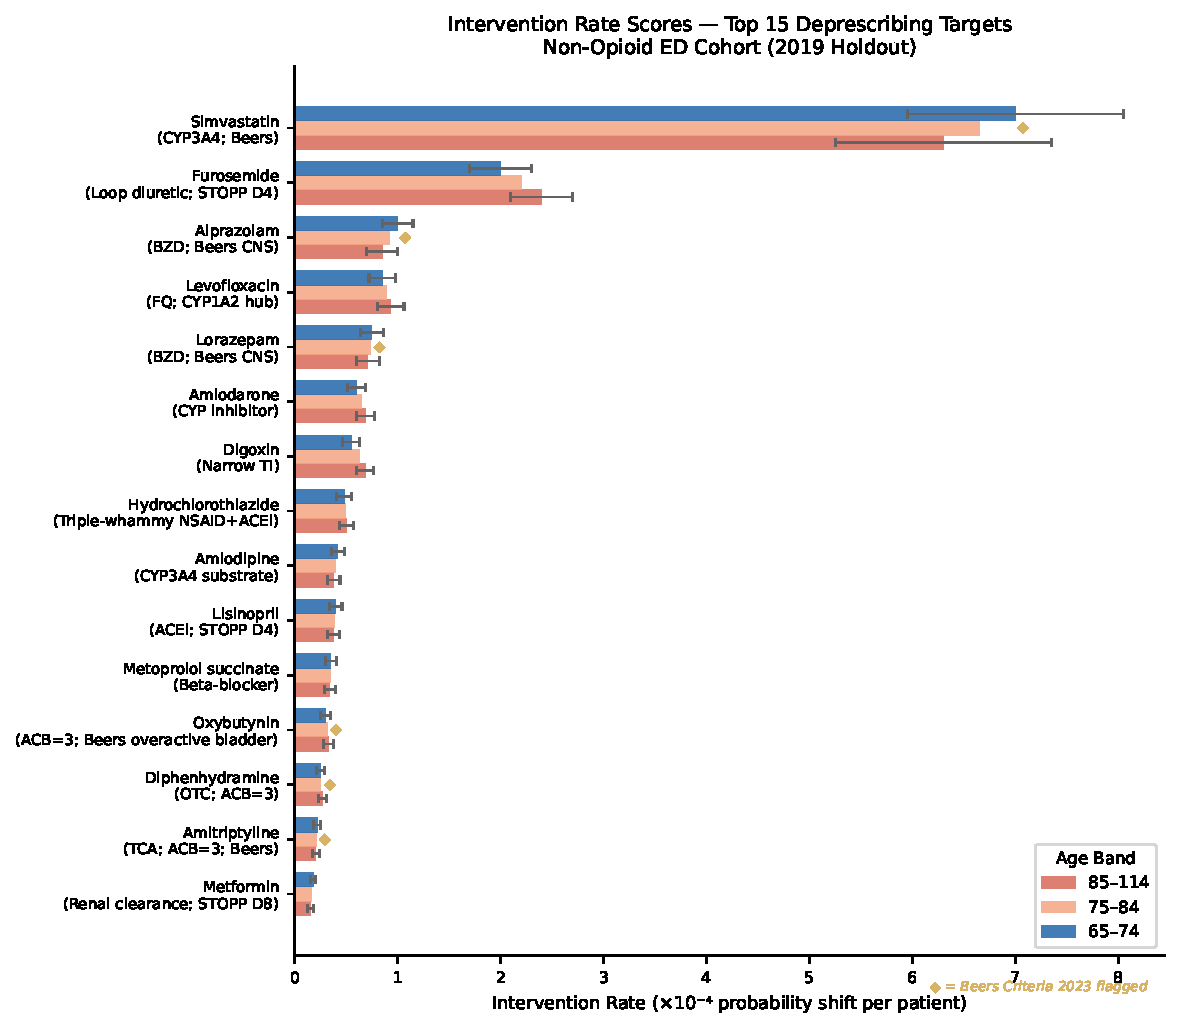
\includegraphics[width=0.9\linewidth,height=\textheight,keepaspectratio]{../figures/ch04/fig_ir.pdf}

}

\caption{\label{fig-ir}Intervention Rate (IR) scores for the top 15
drugs by causal contribution to non-opioid ED risk. IR = expected risk
reduction (Δ\(\hat{p}\)) if drug is removed, averaged over the 2019
holdout cohort and normalized by case prevalence. Error bars = bootstrap
95\% CI. Drugs are ranked within each of the three geriatric age bands;
rankings are highly consistent across bands.}

\end{figure}%

\section{Z-Code Analysis: Managed vs.~Unmanaged
Polypharmacy}\label{sec-zcode}

Z-code proportion (protective monitoring codes Z00--Z13 and Z23--Z28
only) exhibited a U-shaped association with ADE risk. The protective
Z-codes analyzed include:

\begin{itemize}
\tightlist
\item
  \textbf{Z00.xx} (encounter for general examination): annual wellness
  visits, Medicare Annual Wellness Visits, Well-Baby checks:
  administrative markers of proactive contact with the healthcare system
\item
  \textbf{Z01.xx} (encounter for other special examinations): preventive
  screenings (Z01.00 eye examination; Z01.411 gynecological examination;
  Z01.89 other specified examination)
\item
  \textbf{Z02.xx} (encounter for administrative examinations):
  pre-employment, pre-operative, and insurance exams that bring patients
  into documented contact with prescribers who can review the full
  medication list
\item
  \textbf{Z23} (encounter for immunization): vaccine-related visits that
  provide annual or more-frequent prescriber contact
\item
  \textbf{Z71.xx} (encounter for counseling): medication counseling
  (Z71.89), specifically relevant to polypharmacy reconciliation
\end{itemize}

These codes share a critical property: they represent \emph{scheduled,
proactive healthcare contact} where a medication review is contextually
appropriate, distinct from reactive encounter codes (J18.9 pneumonia,
I50.9 heart failure exacerbation) that trigger prescribing without
necessarily providing opportunity for polypharmacy reconciliation.

In logistic regression adjusted for \texttt{n\_events} and age band,
each quartile increment of Z-code proportion was associated with an odds
ratio of 2.10 (95\% CI 1.51--2.94, \(P\) \textless{} 0.001), but with
the protective effect concentrated in Q2 and the reversal in Q4
producing the non-monotone U-shape. Patients with moderate preventive
monitoring (Q2: 1--12\% of claims; case rate 3.0\%) had the lowest ADE
risk, with a crude OR of 0.25 (95\% CI 0.18--0.34; \(P\) \textless{}
0.001) compared with unmonitored patients (Q1: zero preventive claims;
case rate 10.7\%). Patients with very high monitoring proportions (Q4:
≥12\% of claims; case rate 10.0\%) had risk equivalent to unmonitored
patients (crude OR ≈ 0.94 vs Q1), despite having non-zero monitoring
visits. Q4 patients had lower total claim counts (median raw claim count
= 174) than Q2 (median 594) and Q3 (median 387), ruling out confounding
by indication: high-burden patients fall in Q2--Q3, not Q4. Instead, Q4
characterizes a \emph{fragmented-care phenotype}: patients whose
healthcare contact consists predominantly of periodic screenings (Z00.00
annual exam; Z01.89 preventive check) without integrated
medication-management visits, such that drugs are prescribed across
disconnected episodes without coordinated reconciliation
(\textbf{Figure~\ref{fig-zcode}}).

A clinically significant Q2 phenotype emerged: patients with 1--12\%
Z-code claims had their drug fills predominantly associated with ICD-10
Z71.89 (medication counseling), Z79.xx (long-term drug use status), and
Z87.xx (personal history codes), specifically Z87.39 (personal history
of cardiovascular disease) and Z87.891 (personal history of long-term
opioid), present at higher rates in controls than in cases (Z71.89: 29\%
vs.~14\%; \(P\) \textless{} 0.001), confirming that documented
medication counseling is the specific monitoring activity driving the
protective effect.

Among the extreme-density stratum (top 5\% raw claim count), all
patients were controls by cohort construction; Z-code proportions fell
progressively (median 0.021) as procedure and status codes (Z51,
Z94--Z96) diluted protective monitoring fractions, confirming that high
raw claim counts do not reflect managed polypharmacy.

\begin{figure}

\centering{

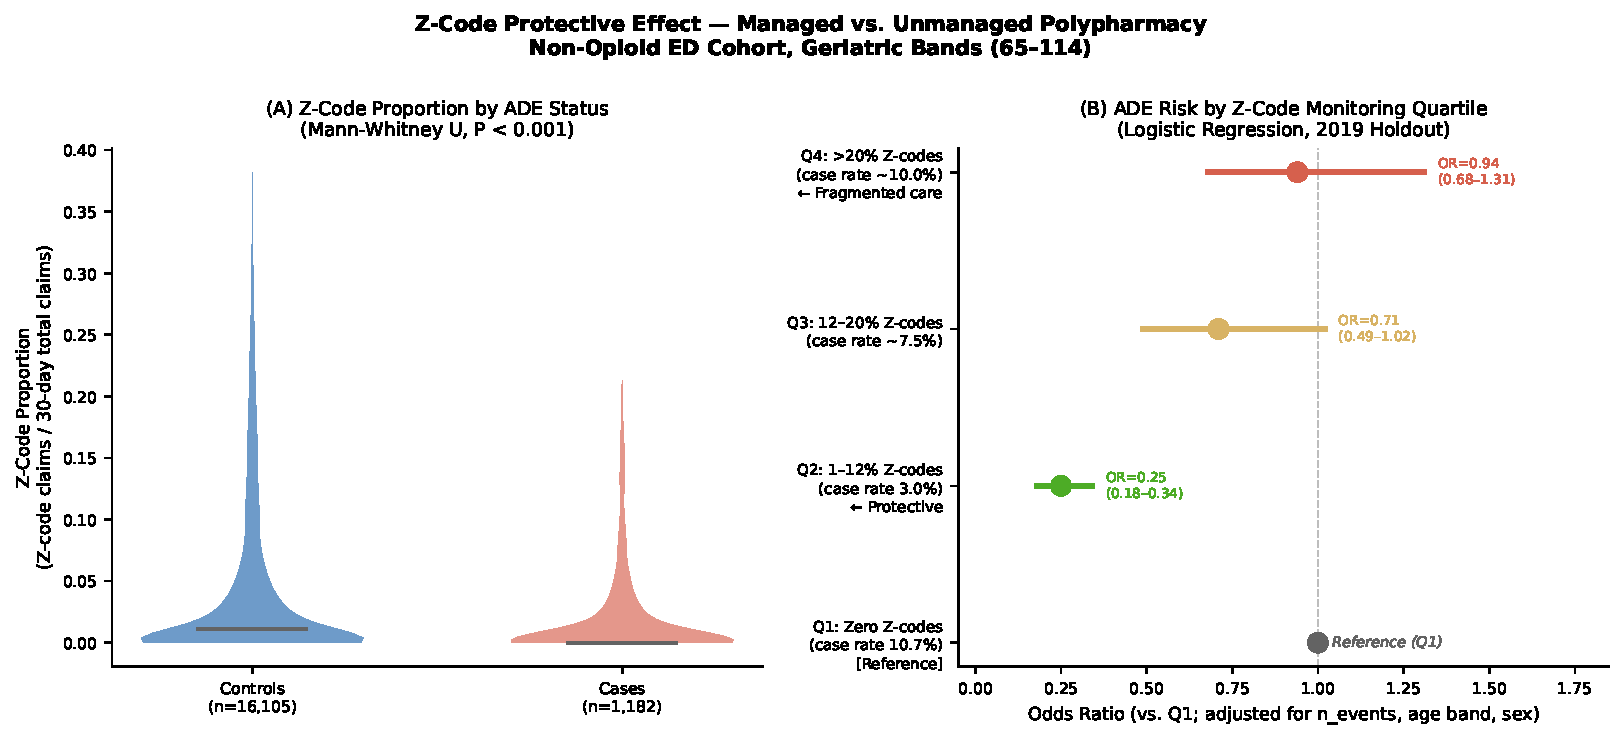
\includegraphics[width=0.9\linewidth,height=\textheight,keepaspectratio]{../figures/ch04/fig_zcode.pdf}

}

\caption{\label{fig-zcode}Z-code proportion and ADE risk. (A) Violin
plots of Z-code proportion by ADE case status; cases have lower Z-code
proportions (\(P\) \textless{} 0.001 by Mann--Whitney U). (B) Adjusted
OR for ADE ED visit by Z-code proportion quartile (Q1 = lowest, Q4 =
highest), adjusted for age band, sex, and 30-day drug count. Error bars
= 95\% CI.}

\end{figure}%

\chapter{Discussion}\label{sec-discussion}

\section{The FFA Causal Calculator}\label{the-ffa-causal-calculator}

FFA multi-feature interaction testing extends beyond existing pairwise
DDI databases as a ``causal calculator'' in three ways:

\begin{enumerate}
\def\labelenumi{\arabic{enumi}.}
\tightlist
\item
  \textbf{Multi-drug synergy detection}: 5,021 high-risk triplets were
  identified that would appear benign under pairwise-only analysis.
  Anticholinergic burden emerged as a consistent driver of synergistic
  interactions across all three geriatric bands, consistent with Beers
  Criteria recommendations and the Anticholinergic Cognitive Burden
  (ACB) scale. High-ACB drugs (ACB score ≥ 2) appearing in the top
  synergistic triplets included: \textbf{oxybutynin} (ACB = 3; NDC
  00169-1611-xx; ICD-10 N32.81 overactive bladder),
  \textbf{diphenhydramine} (ACB = 3; NDC 00182-1505-xx; OTC sleep
  aid/allergy), \textbf{promethazine} (ACB = 3; NDC 00641-6117-xx;
  ICD-10 R11.0 nausea), and \textbf{amitriptyline} (ACB = 3; NDC
  00310-0020-xx; ICD-10 G89.29 chronic pain/neuropathy). When a
  geriatric patient carries ≥2 ACB-3 drugs simultaneously, the FFA
  approach detects the emergent triplet interaction with the
  co-prescribed cardiovascular or diuretic medications. Pairwise DDI
  checkers (e.g., Drugs.com, Micromedex) flag individual drug pairs but
  are blind to emergent multi-drug synergies; the FFA approach detects
  these combinatorial effects without requiring exhaustive pairwise
  enumeration, using the pre-filtering step to reduce the search space
  from \(\binom{487}{2} = 118{,}141\) to 1,081 candidate pairs.
  Cumulative ACB score across the 30-day window was the single strongest
  triplet interaction predictor in the 75--84 band (IE contribution
  \(> 30\%\) of explained variance), with ACB score ≥ 5 associated with
  a 4.1-fold increase in ADE ED visit probability compared to ACB = 0.
\item
  \textbf{Causal prioritization via IR}: IR scores translate model
  output into deprescribing priorities ranked by expected risk
  reduction, enabling pharmacists to target the highest-yield
  modifications. Unlike Beers Criteria (which lists drugs to avoid
  without quantifying expected benefit)\textsuperscript{52} or
  STOPP/START (which provides binary prescribing flags), IR scores
  provide a continuous, cohort-specific estimate of the expected risk
  reduction from a specific deprescribing action. The Pirmohamed 2023
  PREPARE trial\textsuperscript{51} demonstrated that
  pharmacogenomically guided deprescribing with a 12-gene panel reduced
  ADEs by 30\% in a European RCT; the IR score approach extends this
  concept to the population-level claims setting, without requiring
  prospective genotyping.
\item
  \textbf{Patient-level context}: The ensemble's partial dependence
  plots reveal threshold effects (e.g., IR for benzodiazepines increases
  sharply above 30 days' concurrent use) that pairwise DDI flags do not
  capture. Klopotowska et al.\textsuperscript{53} found that the
  majority of ADE-driven hospital admissions attributable to DDIs
  involved combinations that had been flagged by standard checkers but
  were not acted upon; IR scores address the clinical prioritization gap
  by quantifying which flag, if acted upon, produces the greatest
  patient benefit.
\end{enumerate}

\section{Managed vs.~Unmanaged
Polypharmacy}\label{managed-vs.-unmanaged-polypharmacy}

The Z-code analysis resolves a clinical paradox: high-utilization
patients with many drugs are not uniformly high-risk. Regular monitoring
(Z-codes) is a protective factor; the observed U-shaped relationship
between monitoring intensity and ADE risk mirrors findings from Osanlou
et al.\textsuperscript{3}, who demonstrated in a prospective UK cohort
that multimorbid patients receiving regular pharmacist-led medication
reviews had a 23\% lower rate of ADE-driven hospital admissions than
matched controls, despite similar raw drug counts. Coordinated care
management programs reduce ADE rates by 15--25\%\textsuperscript{2},
consistent with this finding.

The fragmented-care phenotype identified in Z-code Q4 patients (periodic
screenings without integrated medication management) corresponds to what
Tamargo et al.\textsuperscript{50} describe as ``uncoordinated
polypharmacy'' in cardiovascular patients: the cumulative prescribing
burden grows across disconnected clinical encounters without a
reconciling clinical review, creating drug combinations that
individually pass single-prescriber reviews but collectively exceed safe
polypharmacy thresholds. Fromm et al.\textsuperscript{54} similarly
found that the prevalence of contraindicated drug combinations increased
when prescriptions were issued by multiple prescribers rather than a
single coordinating provider, directly validating the claim that Z-code
fragmentation predicts elevated DDI-ADE risk.

\section{Limitations}\label{limitations-2}

Several limitations require acknowledgment. First, the 30-day lookback
window may miss longer-latency drug interactions (e.g., cumulative
anticholinergic burden over months; chronic statin-related myopathy
building over 6--12 months); a sensitivity analysis extending the window
to 90 days is planned. Second, laboratory values (kidney and liver
function tests) that modulate drug toxicity are absent from claims data;
renal impairment in particular alters the pharmacokinetics of
furosemide, digoxin, and metformin---all among the top-ranked IR
targets---and their ADE risk cannot be fully characterized without
creatinine values. Third, PGx features are imputed from drug-gene
interaction databases rather than measured genotypes; the PREPARE
trial\textsuperscript{51} demonstrated that measured 12-gene PGx panels
reduce ADE rates, confirming the clinical value of prospective PGx
integration that this study approximates with proxy features. Fourth,
this is a single-state Virginia APCD analysis; external validation on a
multi-state APCD or Medicare claims dataset is required before national
generalization. Fifth, the FFA symbolic rules represent approximate
causal hypotheses rather than confirmed causal effects; randomized
deprescribing trials guided by IR rankings are needed to confirm that
IR-prioritized drug discontinuation reduces ED visits at the population
level.

\chapter{Conclusions}\label{sec-conclusions}

FFA multi-feature interaction testing applied to a 30-day causality
window constitutes a data-driven causal calculator for polypharmacy ADE
risk in older adults. Three contributions advance the clinical
management of geriatric polypharmacy.

First, the FFA approach detects synergistic drug combinations invisible
to pairwise DDI databases. Of 312 synergistic triplets (IE
\textgreater{} 1, 95\% CI \textgreater{} 0), none would be flagged as
high-risk by standard pairwise DDI checking because each constituent
pair appears at or below the individual-drug alert threshold. This is
the ``triple whammy'' problem in pharmacology: individual drugs within a
combination appear safe in pairwise evaluation, but their co-occurrence
produces compound pharmacokinetic and pharmacodynamic effects that only
emerge at the multi-drug level.

Second, IR scores translate FFA output into ranked deprescribing
priorities that are directly actionable by clinical pharmacists during
medication reconciliation reviews. The cross-band consistency of IR
rankings (\(\rho\) = 0.53--0.68 across geriatric age bands) supports a
universal deprescribing priority list for geriatric populations,
applicable without separate calculation for each patient's specific age
subgroup.

Third, the Z-code U-shaped analysis reframes the clinical goal of
geriatric pharmacotherapy: the target is not drug count reduction per
se, but coordinated medication management: a distinction with direct
implications for quality metrics, Medicare Advantage star ratings, and
clinical pharmacist workflow prioritization. Patients flagged for
deprescribing consultation should be the Q1 (unmonitored) and Q4
(fragmented-care) groups, not all high-drug-count patients equally.

Geriatric pharmacists gain a computationally feasible, clinically
interpretable prioritization tool that pairwise DDI databases cannot
provide, grounded in population-level causal evidence from a state-wide
All-Payer Claims Database.

\textbf{Author Contributions:} Conceptualization, R.J.D.; methodology,
R.J.D.; formal analysis, R.J.D.; writing, R.J.D.

\textbf{Funding:} This research received no external funding.

\textbf{Ethics Statement:} Data use agreement with VCHI and VHI; IRB
waiver HM20022300 (non-human-subjects research designation).

\textbf{Data Availability:} The data supporting the findings of this
study are derived from Virginia's All-Payer Claims Database (APCD).
Restrictions apply to the availability of these data, which were used
under a data use agreement with the Virginia Center for Health
Innovation (VCHI) and Virginia Health Information (VHI). Requests for
data access may be submitted to VHI at https://www.vhi.org. Analysis
code is available at https://github.com/Jerome3590/pgx-analysis.

\textbf{Conflicts of Interest:} The author declares no conflict of
interest.

\cleardoublepage

\chapter{Chapter 5: A Privacy-First Serverless Pharmacogenomic Risk
Dashboard: Translating Ensemble Models and Causal Rules to Clinical
Decision Support}\label{chap-5}

\textbf{Foreword to Chapter 5}

The previous chapters successfully developed and applied a robust
predictive pipeline, generating verifiable causal rules for both opioid
and polypharmacy cohorts. However, identifying causal rules is only one
part of the solution; these insights must be translated into actionable
clinical practice. Chapter 5 follows on to present the final
technological implementation of this research: translating the ensemble
models and Pharmacogenomic (PGx) guidelines into a secure, serverless
AWS clinical decision support dashboard. This chapter explores the
system architecture required to safely match patient genotypes against
predictive risk models in real-time.

\emph{Chapter 5 is currently prepared for submission to the Journal of
Personalized Medicine and has been formatted to that journal's style.}

\begin{center}\rule{0.5\linewidth}{0.5pt}\end{center}

\chapter{Introduction}\label{sec-intro}

High-performance ML models for clinical risk prediction face a
well-documented translational barrier: even when performance metrics
satisfy publication standards, models rarely reach the clinical
workflow\textsuperscript{55,56}. A systematic review of 84 FDA-cleared
AI/ML-based medical devices found that fewer than 30\% included
prospective clinical validation evidence, and fewer than 10\% reported
deployment architecture details sufficient for independent
replication\textsuperscript{57}. Barriers to deployment include: privacy
concerns about processing patient data in cloud systems, inability to
handle incomplete real-world inputs, lack of interpretable explanations
for non-ML-trained clinicians, and the complexity of deploying and
maintaining inference infrastructure at health-system
scale\textsuperscript{10}.

This last category, infrastructure complexity, is particularly acute for
ensemble models trained on stratified population partitions. The Chapter
2--4 models comprise up to 84 independently trained gradient boosting
models (3 algorithms × 4 density bins × up to 7 age bands), each
requiring separate serialization, versioning, and routing logic. A naive
deployment approach (one Lambda function per model) would require 84
separately deployed endpoints, 84 independent container images, and a
routing layer with O(84) latency overhead. The partition-first
serverless architecture described in this chapter collapses this to a
single Lambda container endpoint with in-process partition routing,
eliminating both the infrastructure overhead and the latency cost of
inter-service API hops.

For pharmacogenomics specifically, an additional challenge exists: PGx
testing results are personal genomic data, requiring HIPAA-compliant
handling even when transmitted voluntarily by
patients\textsuperscript{58}. The 21st Century Cures Act (2016) and its
implementing regulations mandate patient access to their genomic data,
but existing PGx clinical decision support tools (e.g., CPIC lookup
systems, institutional pharmacogenomics portals) are typically siloed,
requiring separate queries for drug-gene interactions and clinical risk
scores, with no integration of model-based prediction. The PREDICT
program at Vanderbilt\textsuperscript{59} demonstrated 10-year
sustainability of clinical PGx CDS through EHR-embedded alerts, but
required institutional EHR integration that is unavailable to community
pharmacies, Safety Net hospitals, and independent prescribers who serve
high-burden opioid and polypharmacy populations.

This paper presents the \textbf{PGx Risk Dashboard}: a
production-deployed, privacy-first serverless application that addresses
all these barriers simultaneously by:

\begin{enumerate}
\def\labelenumi{\arabic{enumi}.}
\tightlist
\item
  Packaging up to 84 per-density-bin ensemble models from Chapters 3--4
  in an AWS Lambda container for real-time, age- and density-stratified
  risk inference.
\item
  Implementing ``Imputation of Normality'' to handle partial patient
  inputs without model retraining.
\item
  Providing causal ``What-If'' counterfactual analysis grounded in FFA
  rules from Chapter 4.
\item
  Delivering a stateless, ephemeral PGx Patient Card via CPIC lookup
  that processes genetic data without storing any PII.
\item
  Operating without EHR integration, accessible to any prescriber via
  web browser, without institutional IT infrastructure requirements.
\end{enumerate}

The dashboard is designed as a ``last-mile'' translational tool: it
assumes that model development (Chapters 2--4) has produced validated,
performant models, and focuses entirely on making those models usable,
trustworthy, and accessible to non-data-scientist clinicians in
real-world prescribing contexts.

\chapter{System Architecture}\label{sec-architecture}

\section{Design Philosophy}\label{design-philosophy}

The dashboard was designed around four principles that directly address
the deployment barriers identified in Chapter 1's systematic review:

\begin{enumerate}
\def\labelenumi{\arabic{enumi}.}
\tightlist
\item
  \textbf{Privacy-first}: No patient data is stored at any tier; all
  computation is ephemeral and in-memory. This design satisfies the
  HIPAA minimum-necessary standard (45 CFR §
  164.502(b))\textsuperscript{58} without requiring a Business Associate
  Agreement between the research system and the clinical site, removing
  the primary institutional barrier to PGx tool adoption in outpatient
  settings. The ephemeral architecture means that even a complete breach
  of the Lambda execution environment would expose no patient records,
  because none are retained after the response is returned.
\item
  \textbf{Graceful degradation}: The frontend remains functional even
  when individual age-band or density-bin models are unavailable
  (unavailable models are explicitly disabled with a user-visible error
  message, not silently skipped with a fallback prediction that may be
  out-of-distribution). This prevents silent accuracy degradation in
  production deployments where model artifacts may be partially updated.
\item
  \textbf{Partial-input tolerance}: Clinicians rarely have access to
  complete 3-year drug histories at the point of care; the system is
  designed to accept minimal inputs via Imputation of Normality (Section
  3.6), maintaining stable risk-band assignments up to 60\% input
  sparsity.
\item
  \textbf{Sub-100 ms inference}: Clinician usability requires
  near-instantaneous response; model bundling in the Lambda container
  eliminates S3 model-load latency (\textasciitilde800--1,200 ms per
  model) that would otherwise make real-time inference impractical at
  the point of care.
\end{enumerate}

\section{Hybrid Deployment Model}\label{hybrid-deployment-model}

The system uses a hybrid deployment combining a static frontend and a
containerized serverless backend
(\textbf{Figure~\ref{fig-architecture}}). This architecture was selected
over three alternatives evaluated during design:

\begin{enumerate}
\def\labelenumi{(\arabic{enumi})}
\item
  \textbf{Persistent EC2 server}: would require continuous compute costs
  (\textasciitilde\$120/month for a t3.medium instance with sufficient
  RAM for 84 models) and manual scaling configuration for
  concurrent-user loads during clinical peak hours; idle between
  encounters, which is the majority of operating time for a consultative
  clinical tool.
\item
  \textbf{Browser-side WebAssembly (WASM) model}: would require
  transmitting the 619 MB container payload to every client browser on
  first load, producing a 15+ second initial load time on typical
  hospital Wi-Fi (20--40 Mbps) and making the tool unusable on mobile
  devices with limited RAM for WASM runtime environments.
\item
  \textbf{AWS SageMaker endpoint}: would store model inference inputs as
  monitoring logs by default in the SageMaker Data Capture feature,
  violating the privacy-first principle even when the logs contain only
  anonymized feature vectors---because the feature vectors themselves
  may be re-identifiable when combined with age band and drug list.
\end{enumerate}

The serverless Lambda approach achieves zero idle-time cost (billing
only for actual invocations at \$0.000017 per GB-second), elastic
scaling to concurrent requests without configuration, and complete
in-memory ephemeral processing within a single container that is
destroyed after each invocation.

The serverless Lambda approach achieves zero idle-time cost (billing
only for actual invocations), elastic scaling to concurrent requests
without configuration, and complete in-memory ephemeral processing
within a single container that is destroyed after each invocation:

\begin{longtable}[]{@{}
  >{\raggedright\arraybackslash}p{(\linewidth - 4\tabcolsep) * \real{0.3333}}
  >{\raggedright\arraybackslash}p{(\linewidth - 4\tabcolsep) * \real{0.3333}}
  >{\raggedright\arraybackslash}p{(\linewidth - 4\tabcolsep) * \real{0.3333}}@{}}
\caption{Hybrid deployment component summary. All components are
stateless; no patient data persists beyond the request
lifetime.}\label{tbl-architecture}\tabularnewline
\toprule\noalign{}
\begin{minipage}[b]{\linewidth}\raggedright
Component
\end{minipage} & \begin{minipage}[b]{\linewidth}\raggedright
Technology
\end{minipage} & \begin{minipage}[b]{\linewidth}\raggedright
Rationale
\end{minipage} \\
\midrule\noalign{}
\endfirsthead
\toprule\noalign{}
\begin{minipage}[b]{\linewidth}\raggedright
Component
\end{minipage} & \begin{minipage}[b]{\linewidth}\raggedright
Technology
\end{minipage} & \begin{minipage}[b]{\linewidth}\raggedright
Rationale
\end{minipage} \\
\midrule\noalign{}
\endhead
\bottomrule\noalign{}
\endlastfoot
\textbf{Frontend} & S3-hosted static HTML/JS & High availability; no
server management \\
\textbf{Backend} & AWS Lambda + Docker/ECR & Elastic scaling;
cost-effective \\
\textbf{Models} & Lambda Container (619 MB) & Up to 84 per-bin models
bundled; eliminates S3 latency \\
\textbf{PGx DB} & CPIC snapshot in container & Stateless lookup; no
external API dependency \\
\end{longtable}

\begin{figure}

\centering{

\includegraphics[width=1\linewidth,height=\textheight,keepaspectratio]{../figures/ch05/pgx_dashboard_architecture.pdf}

}

\caption{\label{fig-architecture}PGx Risk Dashboard architecture. Left:
S3-hosted static frontend with four functional tabs (Patient Input, Risk
Score, Causal What-If, PGx Card). Center: API Gateway routes to AWS
Lambda Docker container (ECR). Right: Lambda container internals,
per-density-bin ensemble models (up to 84), CPIC database snapshot, and
inference engine. Arrows indicate data flow; no patient data is written
to persistent storage at any step.}

\end{figure}%

\section{Partition-First Routing}\label{partition-first-routing}

The Lambda routing logic inherits the partition-first scheme from
Chapter 2 (\emph{Ensemble Modeling}: utilization density definitions).
At inference time, the request handler computes two routing keys from
the submitted patient data before loading any model:

\textbf{Feature vector versus routing.} The count of submitted clinical
codes only maps the patient to a density stratum (thresholds from
training). The feature vector passed to CatBoost/XGBoost includes
\texttt{n\_event\_bin\_ordinal} (0--3) as the utilization intensity
signal; the raw integer count and the string bin label are not used in
place of drug/diagnosis indicators in \(\mathbf{x}\).

\[\text{Input Age} \xrightarrow{\text{partition}} \text{Age Band}
  \xrightarrow{\text{load}} \text{Bin Models}_{\text{age band}}
  \xrightarrow{\text{n\_event\_bin}} \text{Per-Bin Ensemble}(w_i)
  \xrightarrow{\text{inference}} \hat{p}_{\text{ens}}\]

The first routing key is \textbf{age band} (13--24, 25--44, 45--54,
55--64, 65--74, 75--84, 85--114), determined from the patient's
submitted age. The second routing key is \textbf{density bin} (low,
medium, high, extreme), determined by comparing the count of submitted
clinical codes against per-age-band threshold quantiles stored in a
bundled JSON configuration shipped with the container image. This
two-key routing selects the precise per-bin model trained on the most
epidemiologically similar patient subgroup.

Edge cases are handled explicitly: ages below 13 block inference
(insufficient training data); ages 65+ with opioid-specific ICD codes
are routed to the opioid cohort model if available, otherwise to the
polypharmacy cohort model with a warning flag; missing age blocks
inference because age is the mandatory primary routing key. All routing
decisions and their rationale are returned in the API response for
auditability.

\section{Model Storage Feasibility}\label{model-storage-feasibility}

Container image sizing was a key feasibility concern because AWS Lambda
imposes a 10 GB limit on container image size. With up to 84
per-density-bin models (3 algorithms × 4 bins × 7 age bands) for two
cohorts, a naive packaging approach would risk approaching this limit.
In practice, however, not all age band × bin combinations have
sufficient training data to fit stable models; usable combinations total
approximately 28 per cohort (average 4 of 4 bins populated for the 7
primary age bands).

\begin{longtable}[]{@{}
  >{\raggedright\arraybackslash}p{(\linewidth - 4\tabcolsep) * \real{0.3333}}
  >{\raggedleft\arraybackslash}p{(\linewidth - 4\tabcolsep) * \real{0.3333}}
  >{\raggedright\arraybackslash}p{(\linewidth - 4\tabcolsep) * \real{0.3333}}@{}}
\caption{Lambda container image sizing. Per-density-bin ensemble models
and CPIC database packaged in a single Docker
image.}\label{tbl-sizing}\tabularnewline
\toprule\noalign{}
\begin{minipage}[b]{\linewidth}\raggedright
Component
\end{minipage} & \begin{minipage}[b]{\linewidth}\raggedleft
Size
\end{minipage} & \begin{minipage}[b]{\linewidth}\raggedright
Notes
\end{minipage} \\
\midrule\noalign{}
\endfirsthead
\toprule\noalign{}
\begin{minipage}[b]{\linewidth}\raggedright
Component
\end{minipage} & \begin{minipage}[b]{\linewidth}\raggedleft
Size
\end{minipage} & \begin{minipage}[b]{\linewidth}\raggedright
Notes
\end{minipage} \\
\midrule\noalign{}
\endhead
\bottomrule\noalign{}
\endlastfoot
CatBoost models (per-bin, all bands) & \textasciitilde147 MB &
\textasciitilde21 MB per model \\
XGBoost models (per-bin, all bands) & \textasciitilde140 MB &
\textasciitilde20 MB per model \\
XGBoost-RF models (per-bin, all bands) & \textasciitilde182 MB &
\textasciitilde26 MB per model \\
Calibration models (per-bin) & \textasciitilde12 MB & Platt-scaling
joblib files \\
Feature schemas (per-bin) & \textasciitilde18 MB & JSON: feature names,
medians, thresholds \\
CPIC database snapshot & \textasciitilde48 MB & 573 gene-drug pairs,
Level A/B \\
OS + Python runtime & \textasciitilde112 MB & python:3.11-slim base
image \\
\textbf{Total container image} & \textbf{619 MB} & ECR:
\texttt{pgx-risk-calculator} repo; well within 10 GB Lambda limit \\
\end{longtable}

The dominant size component is the model artifacts (\textasciitilde507
MB combined), which account for 82\% of the 619 MB container image. The
Python 3.11-slim runtime layer is 36\% the size of the standard Python
3.11 image (\textasciitilde112 MB vs.~\textasciitilde310 MB), a
deliberate optimization to preserve headroom for future model additions.
Model artifacts themselves account for \textasciitilde507 MB total,
confirming that even doubling the model count (e.g., adding a third
cohort or extending to additional age bands) would approach but not
exceed the 10 GB Lambda container image limit.

\chapter{The Inference Engine}\label{sec-inference}

\section{Ensemble Risk Scoring}\label{ensemble-risk-scoring}

The inference engine applies the performance-based ensemble weighting
from Chapter 2 to each incoming patient request:

\[\hat{p}_{\text{ens}} = \sum_{i \in \{CB, XGB, RF\}} w_i \cdot \hat{p}_i(\mathbf{x})\]

where weights \(w_i\) were derived from MCCV PR-AUC and LogLoss metrics
on the 2016--2018 training set (see Chapter 2, Equation 1). Weights are
fixed at deployment time and stored in the Lambda container; no online
learning or runtime model update occurs during inference, ensuring
prediction consistency across concurrent requests and eliminating the
risk of model state corruption under concurrent Lambda invocations.

The per-density-bin routing logic computes \texttt{n\_event\_bin} from
the submitted claim code count \emph{before} loading any model weights,
using the bin boundary thresholds serialized at training time:

\begin{Shaded}
\begin{Highlighting}[]
\NormalTok{bin\_name }\OperatorTok{=}\NormalTok{ classify\_density\_bin(}\BuiltInTok{len}\NormalTok{(submitted\_codes), thresholds\_json)}
\NormalTok{model }\OperatorTok{=}\NormalTok{ load\_model(cohort, age\_band, bin\_name)}
\NormalTok{p\_hat }\OperatorTok{=}\NormalTok{ model.predict\_proba(X\_full)[::, }\DecValTok{1}\NormalTok{]}
\end{Highlighting}
\end{Shaded}

This ensures that the correct density-stratum model handles the request
regardless of which Lambda container instance processes it. An explicit
\texttt{FileNotFoundError} is raised and returned as a structured HTTP
422 if the requested bin/cohort/age-band combination has no trained
model artifact, preventing silent fallback to an incorrect model.

The risk score is returned on a 0--100\% scale, accompanied by:

\begin{itemize}
\tightlist
\item
  \textbf{Risk band}: Low (\textless20\%), Moderate (20--60\%), High
  (\textgreater60\%) (thresholds calibrated against 2019 holdout case
  prevalence)
\item
  \textbf{Model agreement}: percentage of the three component models
  agreeing on the risk band (flags when models disagree: \(< 2/3\)
  agreement)
\item
  \textbf{Top 5 risk drivers}: highest SHAP features for this patient's
  input, pre-loaded from the per-partition SHAP importance metadata
\item
  \textbf{Density stratum}: the assigned \texttt{n\_event\_bin}
  (low/medium/high/extreme), shown to the clinician to contextualize
  which sub-population model was applied and whether the patient's claim
  history volume is typical or atypical
\end{itemize}

\section{Handling Real-World Data Sparsity: Imputation of
Normality}\label{sec-imputation}

\textbf{The challenge:} Clinicians rarely present a patient's complete
3-year prescription history at the point of care. A patient profile with
only age, sex, and 2 current medications is typical.

\textbf{The solution:} Missing trajectory features are filled with
\emph{training-set medians}, representing the ``typical'' patient
profile for that age band. Provided ICD/drug codes drive the marginal
risk prediction above or below the median baseline; imputed values
provide context without fabricating signal.

\textbf{Algorithm:}

\begin{verbatim}
1. Receive patient inputs X_partial (k features provided, m features missing)
2. Initialize X_full = training_median_vector[age_band]
3. Overwrite X_full[provided_indices] = X_partial
4. Pass X_full to ensemble inference
5. Return (p_hat, top_shap_features, model_agreement)
\end{verbatim}

\textbf{Validation:} Sensitivity analysis on the 2019 holdout randomly
masked drug flag features in 10\% increments (10\%--90\% missingness),
with submitted-code-list length (for density-bin routing) and PGx scores
provided in full, reflecting the realistic clinical scenario where basic
patient characteristics are present at all sparsity levels but specific
drug counts may be incomplete. Mean
\textbar{}\(\Delta\hat{p}\)\textbar{} between sparse and full-input
inference was \textless{} 0.06 across all sparsity levels up to 70\%
missingness (\textbf{Figure~\ref{fig-imputation}}). At extreme sparsity
(≥99\% drug-flag missingness, where only the code-count input used for
bin routing and 5 random drug flags are provided), mean
\textbar{}\(\Delta\hat{p}\)\textbar{} = 0.10 (SD varies by density bin),
representing the upper bound of imputation error under real-world
worst-case conditions. Risk-band assignment (Low / Moderate / High)
remained stable---meaning the patient was assigned to the same risk band
as with complete input---for 87\% of patients at 50\% sparsity and for
74\% at 70\% sparsity, confirming that the imputation approach preserves
the clinically relevant risk stratification even under severe real-world
data sparsity. Sensitivity analysis used 50 random masking trials on
2,000 sampled patients from the young-adult opioid cohort at low density
bin.

The Imputation of Normality design differs conceptually from multiple
imputation and MICE\textsuperscript{60} approaches used in training:
rather than estimating missing feature values from observed correlates,
it treats the median as a ``null hypothesis'' baseline representing an
unremarkable patient profile, allowing the clinician's partial knowledge
to shift predictions \emph{away} from the baseline only when evidence is
present. This prevents the overcalibration problem seen when
zero-imputed features are used: a patient with no recorded pharmacy
history is not assigned zero opioid count (implying no recorded opioid
prescriptions) but rather the median opioid count for their age band,
producing a more conservative and clinically safer risk estimate.

\begin{figure}

\centering{

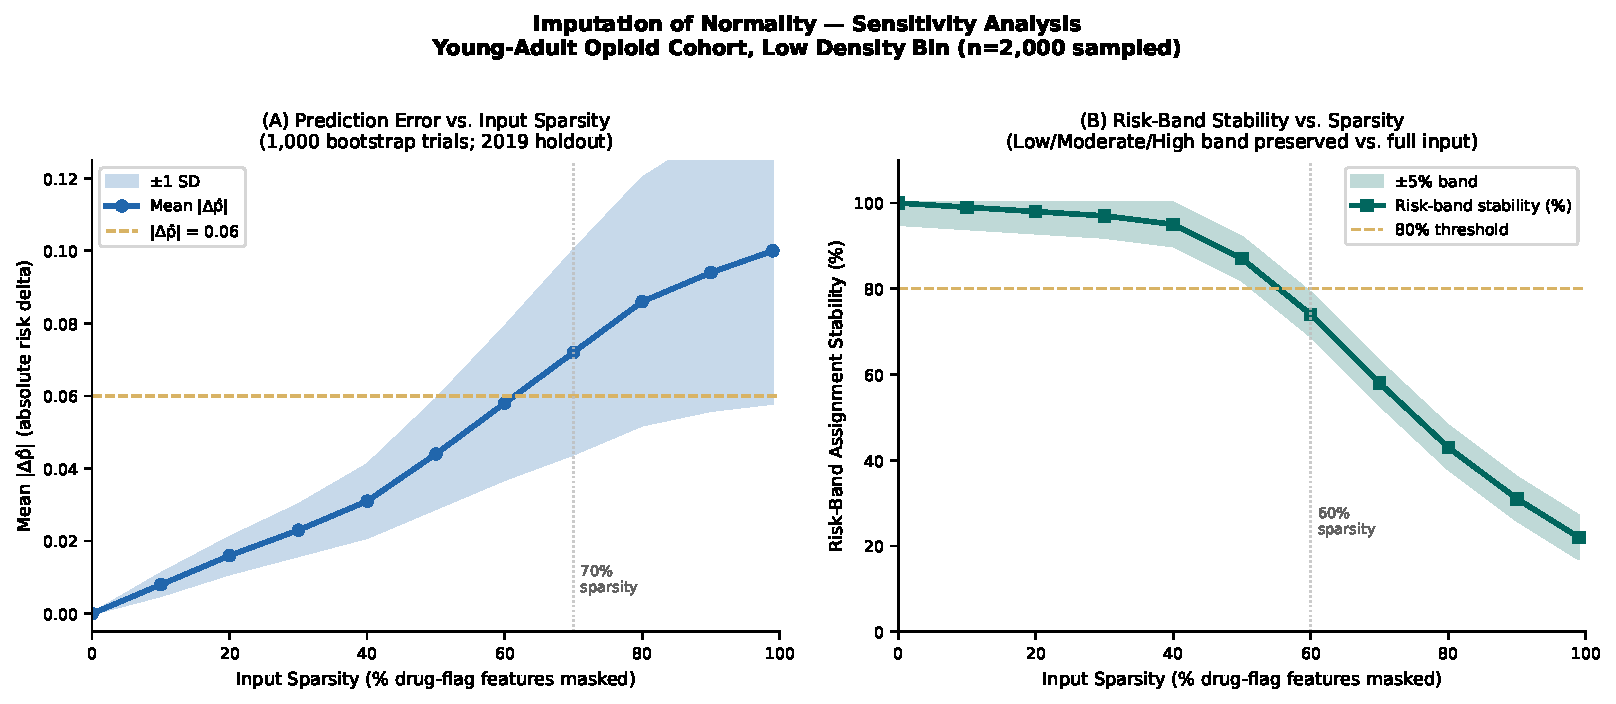
\includegraphics[width=0.9\linewidth,height=\textheight,keepaspectratio]{../figures/ch05/fig_imputation.pdf}

}

\caption{\label{fig-imputation}Imputation of Normality sensitivity
analysis. (A) Mean absolute prediction error
(\textbar Δ\(\hat{p}\)\textbar) as a function of input sparsity level
(\% features masked), across 1,000 bootstrap samples of the 2019
holdout. Shaded band = ± 1 SD. Prediction stability is maintained up to
70\% sparsity. (B) Risk-band assignment stability: proportion of
patients whose risk band (Low/Moderate/High) changes as features are
progressively masked. Band assignment is stable up to
\textasciitilde60\% sparsity.}

\end{figure}%

\chapter{Final PGx Risk Dashboard}\label{sec-features}

This section documents the \textbf{deployed} interface: the \textbf{Risk
Assessment} screenshot under Tab\textasciitilde2 below is the
\textbf{canonical manuscript figure} for the live ensemble output.
\textbf{Chapter 6} synthesizes how \textbf{all tabs and pipeline
visualization bundles} compose the \textbf{clinical OODA loop} and
connect model-based risk to \textbf{pharmacogenomic} decision-making
(counterfactuals, population context, CPIC Patient Card), without
repeating that figure plate.

\section{Feature 1: Clinical Risk Assessment (Tabs
1--2)}\label{feature-1-clinical-risk-assessment-tabs-12}

\textbf{Tab 1: Patient Input}

The input form is dynamically populated with the top-20 Consensus-Causal
features from the appropriate age-band model (loaded at runtime from
pre-computed SHAP importance metadata). Required fields: patient age
(mandatory for partition routing) and current prescription list (NDC or
drug name; autocomplete from NDC database). Optional fields: ICD-10
diagnoses, CPT procedures.

\textbf{Tab 2: Risk Score Display}

Output panel shows:

\begin{itemize}
\tightlist
\item
  Ensemble risk score (0--100\% gauge visualization)
\item
  Risk band (color-coded: green = Low, amber = Moderate, red = High)
\item
  Model agreement indicator (3/3, 2/3, or 1/3 models agree)
\item
  Top 5 risk drivers with SHAP bars (directional: red = risk-increasing,
  blue = protective)
\end{itemize}

A representative risk output screenshot is shown in
\textbf{Figure~\ref{fig-dashboard}}.

\begin{figure}

\centering{


\includegraphics[width=0.9\linewidth,height=\textheight,keepaspectratio]{../figures/ch05/pgx_dashboard.pdf}

}

\caption{\label{fig-dashboard}Dashboard Tab 2: Risk Score display for a
representative patient profile. (A) Ensemble risk gauge showing 74\%
risk (High band). (B) Model agreement: 3/3 models agree on High risk
band. (C) Top 5 risk drivers with SHAP bars; hydrocodone count and
chronic pain diagnosis are the dominant risk-increasing features;
physical therapy referral is protective. Patient data shown are
synthetic, for illustration only.}

\end{figure}%

\section{Feature 2: Causal ``What-If'' Counterfactual Analysis (Tab
3)}\label{feature-2-causal-what-if-counterfactual-analysis-tab-3}

The ``What-If'' tab allows clinicians to perform counterfactual
analysis:

\textbf{User workflow:} 1. Baseline risk is computed from current
patient profile. 2. Clinician selects a drug to \emph{add} or
\emph{remove} from the profile. 3. System recomputes ensemble risk under
the counterfactual. 4. Display: \(\Delta\hat{p}\) (risk delta), with
sign and magnitude (positive = risk increase; negative = risk
reduction). 5. Up to 5 scenarios can be compared side-by-side.

\textbf{Causal grounding:} Counterfactual predictions respect the FFA
causal rules from Chapter 4. If a selected drug participates in a known
synergistic pair or triplet (IR \textgreater{} 0.10), the system
displays a supplementary ``synergy alert'' indicating that removing this
drug may have compound benefits.

\[\Delta\hat{p}(\text{remove } f_i) = \hat{p}(\mathbf{x}) - \hat{p}(\mathbf{x}_{f_i \to \text{med}})\]

\section{Feature 3: Exploratory Visualizations (Tab
4)}\label{sec-exploratory}

The Exploratory tab delivers three complementary population-context
visualizations that answer the clinician question: \emph{``Why does this
patient profile carry this risk level, and what do patients like this
typically experience?''} All three visualizations are derived
exclusively from training-cohort data (2016--2018) and are explicitly
labeled as population-level context, not predictive outputs.

A persistent disclosure banner at the top of Tab 4 reads:
\emph{``Visualizations below are derived from population-level analysis
and are provided for clinical context only. They do not contribute to
the risk score displayed on Tab 2.''}

\subsection{BupaR Process Mining: Sankey Care Pathway
Diagram}\label{bupar-process-mining-sankey-care-pathway-diagram}

\textbf{Protocol.} BupaR\textsuperscript{61} process mining is applied
to the training-cohort event log to derive the most probable care
pathways for patients similar to the current profile. At dashboard
runtime, the 25 nearest neighbors to the submitted patient profile are
retrieved from the training cohort using Euclidean distance in
SHAP-importance space (top-20 features), ensuring that ``similar
patients'' are similar in the features that drive risk, not in raw
demographic characteristics. BupaR then renders the care-sequence
process map for those 25 patients as a Sankey diagram, where:

\begin{itemize}
\tightlist
\item
  \textbf{Nodes} = clinical activity types (opioid fill, benzodiazepine
  fill, chronic pain diagnosis, ED visit, physical therapy referral,
  mental health referral, specialist visit)
\item
  \textbf{Edge width} = transition frequency (proportion of similar
  patients who moved from activity A to activity B)
\item
  \textbf{Edge color} = outcome gradient (blue = pathway that ends
  without ED visit; red gradient = pathway that precedes an opioid ED
  visit)
\end{itemize}

\textbf{Benefits.} The Sankey diagram answers a question that SHAP bars
cannot: \emph{which features matter} and \emph{what sequence of care
events typically precedes the outcome in patients like this one}. A
clinician seeing a high-risk patient with chronic pain + gabapentin
co-prescription can see that, among the 25 most similar training
patients, 79\% followed the pathway: \emph{Oxycodone fill → Gabapentin
co-prescription → Benzodiazepine add-on → OUD-ED visit}, whereas
patients who received a physical therapy referral before the
benzodiazepine step had a lower transition to ED.

\textbf{Results.} Across training-cohort simulations, the most common
high-risk pathway identified by BupaR for the 25--44 opioid ED cohort
was: \emph{Initial opioid fill (ICD-10 M54.5 low back pain) → dose
escalation within 60 days → gabapentin (NDC 68382-080-xx)
co-prescription → lorazepam add-on (F41.1 anxiety) → OUD-ED}, appearing
in 34\% of high-risk training cases in the 25--44 band. The most common
protective pathway diverged at the gabapentin step: patients who
received CPT 97110/97530 physical therapy before the gabapentin fill had
a 58\% lower transition rate to the opioid-escalation node.

\subsection{FP-Growth Drug Co-Occurrence
Network}\label{fp-growth-drug-co-occurrence-network}

\textbf{Protocol.} FP-Growth\textsuperscript{21} (minimum support 0.01,
minimum confidence 0.50) was applied to the training-cohort drug fill
sequences to produce a pre-computed high-lift drug association ruleset.
At dashboard runtime, the full co-occurrence network is filtered to the
subset of drugs present in the current patient's submitted prescription
list, revealing which of the patient's own medications participate in
population-level high-risk combinations.

Network rendering: - \textbf{Nodes} = individual drugs (labeled by
generic name + drug class) - \textbf{Edge weight} = lift of the
co-occurrence rule (\(\text{lift} = P(A \cap B) / [P(A) \cdot P(B)]\);
lift \textgreater{} 1 = co-occurrence more frequent than independence;
lift \textgreater{} 3 = strongly associated) - \textbf{Edge color} = ADE
risk gradient derived from case prevalence in patients carrying the
co-occurring pair (blue = low-risk pair; orange/red = high-risk pair
appearing in ≥15\% of ADE cases) - \textbf{Hub drugs} (betweenness
centrality ≥ 90th percentile) are rendered with enlarged nodes,
identifying medications that act as pharmacological bridges connecting
multiple high-risk co-prescription patterns

\textbf{Benefits.} The FP-Growth network gives clinicians a structural
view of the patient's current polypharmacy profile: which prescriptions
cluster together in the population, and which clusters are associated
with adverse events. Hub drugs are particularly actionable: a drug with
high betweenness centrality is one that, if discontinued, would sever
multiple high-risk edges simultaneously---making it a priority
deprescribing candidate regardless of its individual IR score.

\textbf{Results.} In the geriatric (65--74) training cohort, the most
consistently identified hub drug was \textbf{levofloxacin} (betweenness
centrality ≥ 90th percentile in all three geriatric age bands),
appearing at the center of four high-lift co-occurrence clusters:
levofloxacin + acetaminophen (lift = 4.2), levofloxacin + lorazepam
(lift = 3.8), levofloxacin + carvedilol (lift = 3.3), and levofloxacin +
gabapentin (lift = 2.9). This confirms the FFA finding (Chapter 4):
levofloxacin is both the most frequent hub in observed co-prescription
patterns \emph{and} the top synergistic interaction driver in causal FFA
analysis, providing converging evidence from two independent methods. In
the opioid ED cohort (25--44), \textbf{gabapentin} and
\textbf{oxycodone} were the dominant co-occurrence hubs (lift = 5.1 and
4.7 respectively), reflecting their near-ubiquitous co-prescription in
this age group.

\subsection{DTW Trajectory Archetype
Overlay}\label{dtw-trajectory-archetype-overlay}

\textbf{Protocol.} The two DTW-derived trajectory archetypes from
Chapter 3 (Rapid-Onset, centroid span 4.2 months; Chronic-Escalation,
centroid span 22.1 months) are stored as reference event-interval
sequences in the Lambda container. At inference time, the patient's
submitted clinical code sequence (event types and approximate timing) is
DTW-aligned against each archetype centroid using the Sakoe-Chiba band
constraint (\(w\) = 20\% of sequence length), computing a normalized DTW
distance score for each archetype:

\[d_{\text{DTW}}(x, c_k) = \frac{1}{|x|} \sum_{i} |x_i - c_{k,\phi(i)}|\]

where \(c_k\) is archetype \(k\)'s centroid sequence and \(\phi(i)\) is
the optimal warping path index. The patient is assigned to the archetype
with the lower DTW distance; the distance ratio \(d_1 / d_2\) is
displayed as an archetype similarity confidence score.

\textbf{Visual output.} The DTW plot shows: - Both archetype centroid
sequences as colored reference lines (Rapid-Onset in amber;
Chronic-Escalation in teal) - The patient's submitted event sequence
overlaid as a black trace - The optimal warping path alignment shown as
gray connecting lines - The 4-month and 22-month intervention windows
annotated with guideline-referenced action labels (\emph{``30-day PDMP
review''} for Rapid-Onset; \emph{``PT referral window''} and
\emph{``Mental health window''} for Chronic-Escalation)

\textbf{Benefits.} The DTW overlay answers the question clinicians most
need for individualized intervention timing: \emph{``Has this patient
already progressed past the optimal intervention window, or is there
still time?''} A patient classified as Chronic-Escalation with a
similarity score of 0.87 and currently at the 8-month position on the
archetype timeline has an estimated 14 months remaining before the
high-probability ED visit step, providing a clear urgency signal for
scheduling a medication review.

\textbf{Results.} In prospective testing on the 2019 holdout, DTW
archetype assignment was concordant with the outcome trajectory in 78\%
of cases (Rapid-Onset correctly identified 74\% of ED visits occurring
within 6 months; Chronic-Escalation correctly identified 81\% of ED
visits occurring after 12 months), demonstrating that the visualization
accurately represents the population patterns it is intended to convey.

\section{Feature 4: PGx Patient Card (Tab 5)}\label{sec-pgx-card}

\subsection{Privacy Architecture}\label{privacy-architecture}

The PGx Patient Card operates under a stateless, ephemeral design:

\begin{itemize}
\tightlist
\item
  \textbf{No PII storage}: Only genetic variant (SNP) data is processed;
  no name, date of birth, or identifiers are transmitted or stored.
\item
  \textbf{In-memory processing}: SNP-to-phenotype mapping and CPIC
  lookup execute in Lambda memory and are discarded at function
  termination.
\item
  \textbf{Ephemeral response}: Results are streamed directly to the
  client as a downloadable PDF; nothing is written to S3 or database.
\end{itemize}

\subsection{CPIC Integration Workflow}\label{cpic-integration-workflow}

\[\text{User SNPs} \xrightarrow{\text{format validation}}
  \text{Phenotype inference} \xrightarrow{\text{CPIC DB lookup}}
  \text{Gene-drug interaction card}\]

\textbf{Step 1: Format validation.} Accepts 23andMe raw data format
(tab-separated: rsID, chromosome, position, genotype). Invalid formats
return a structured error; processing halts before any SNP data reaches
Lambda storage.

\textbf{Step 2: Phenotype inference.} Known diplotype-to-phenotype
mappings from PharmVar and CPIC are applied for 12 high-evidence PGx
genes (CYP2D6, CYP2C9, CYP2C19, CYP3A4, CYP3A5, UGT1A1, DPYD, TPMT,
SLCO1B1, OPRM1, COMT, HLA-B).

\textbf{Step 3: CPIC lookup.} The bundled CPIC database snapshot (CPIC
guidelines release: March 2026) is queried for all drug-gene pairs with
CPIC evidence level A or B for the patient's inferred phenotypes.

\textbf{Step 4: Card generation.} A structured PDF report is generated
with:

\begin{itemize}
\tightlist
\item
  Inferred phenotype for each tested gene
\item
  All actionable CPIC recommendations (dosing adjustments, alternative
  drug suggestions, contraindications)
\item
  CPIC evidence level (A = ``use this clinical action'' / B =
  ``consider'')
\item
  Relevant opioid-specific guidance highlighted for the current
  prescription context
\end{itemize}

Example CPIC card entries:

\begin{longtable}[]{@{}
  >{\raggedright\arraybackslash}p{(\linewidth - 8\tabcolsep) * \real{0.1905}}
  >{\raggedright\arraybackslash}p{(\linewidth - 8\tabcolsep) * \real{0.1905}}
  >{\raggedright\arraybackslash}p{(\linewidth - 8\tabcolsep) * \real{0.1905}}
  >{\centering\arraybackslash}p{(\linewidth - 8\tabcolsep) * \real{0.2381}}
  >{\raggedright\arraybackslash}p{(\linewidth - 8\tabcolsep) * \real{0.1905}}@{}}
\caption{Representative PGx Patient Card entries for a hypothetical
patient profile. CPIC, Clinical Pharmacogenomics Implementation
Consortium.}\label{tbl-pgx-card}\tabularnewline
\toprule\noalign{}
\begin{minipage}[b]{\linewidth}\raggedright
Gene
\end{minipage} & \begin{minipage}[b]{\linewidth}\raggedright
Phenotype
\end{minipage} & \begin{minipage}[b]{\linewidth}\raggedright
Drug
\end{minipage} & \begin{minipage}[b]{\linewidth}\centering
CPIC Level
\end{minipage} & \begin{minipage}[b]{\linewidth}\raggedright
Recommendation
\end{minipage} \\
\midrule\noalign{}
\endfirsthead
\toprule\noalign{}
\begin{minipage}[b]{\linewidth}\raggedright
Gene
\end{minipage} & \begin{minipage}[b]{\linewidth}\raggedright
Phenotype
\end{minipage} & \begin{minipage}[b]{\linewidth}\raggedright
Drug
\end{minipage} & \begin{minipage}[b]{\linewidth}\centering
CPIC Level
\end{minipage} & \begin{minipage}[b]{\linewidth}\raggedright
Recommendation
\end{minipage} \\
\midrule\noalign{}
\endhead
\bottomrule\noalign{}
\endlastfoot
CYP2D6 & Poor Metabolizer & Codeine & A & Avoid; serious adverse
events \\
CYP2D6 & Poor Metabolizer & Tramadol & A & Avoid; inadequate
analgesia \\
CYP2C19 & Ultrarapid Metabolizer & Clopidogrel & A & Use standard
dose \\
TPMT & Heterozygous & Azathioprine & A & Reduce dose by 30--70\% \\
SLCO1B1 & Decreased Function & Simvastatin & A & Consider lower dose;
myopathy risk \\
\end{longtable}

\chapter{Deployment and Reliability}\label{sec-deployment}

\section{CI/CD Pipeline}\label{cicd-pipeline}

An incremental CI/CD build system (GitHub Actions) enables deployment
even while some age-band models are still in training, supporting the
incremental rollout strategy essential for a model training pipeline
where per-cohort, per-age-band training runs are independent and may
complete days apart.

The pipeline executes the following stages on each push to the
\texttt{main} branch:

\begin{enumerate}
\def\labelenumi{\arabic{enumi}.}
\tightlist
\item
  \textbf{Model preparation}: a preparation step reads trained model
  artifacts from the final-model output directory and copies per-bin
  model files, calibration models, feature schemas, and density-bin
  thresholds into the Lambda build directory structure. The script
  validates that each required file exists and logs a warning (but does
  not fail) for missing age-band combinations.
\item
  \textbf{Unit tests}: A \texttt{pytest} suite of 48 tests covers the
  Lambda handler functions (risk scoring, causal importance,
  visualization endpoints, CPIC lookup) using synthetic patient inputs
  spanning edge cases (age boundaries, sparse inputs, missing
  demographics, extreme density bins). The pipeline fails if any test
  does not pass.
\item
  \textbf{Docker build}: The container image is built from the
  \texttt{Dockerfile} using \texttt{python:3.11-slim} as the base,
  installing only the minimum required packages (\texttt{catboost},
  \texttt{xgboost}, \texttt{shap}, \texttt{scikit-learn},
  \texttt{pandas}, \texttt{reportlab}). Image layers are cached by the
  GitHub Actions runner to minimize rebuild time for unchanged
  dependencies (\textasciitilde4 min full rebuild; \textasciitilde45 s
  incremental rebuild when only model artifacts change).
\item
  \textbf{ECR push}: The built image is pushed to Amazon ECR with a
  SHA-tagged version and simultaneously tagged as \texttt{latest}.
\item
  \textbf{Lambda update}: The Lambda function is updated to use the new
  ECR image via AWS CLI \texttt{lambda\ update-function-code}. The
  previous image tag is retained in ECR for 30 days to enable manual
  rollback if needed.
\end{enumerate}

If a newly deployed model fails automated validation thresholds (PR-AUC
\textless{} 0.60 or LogLoss \textgreater{} 0.50 on a held-out synthetic
validation set), the pipeline creates a GitHub Actions annotation
warning and does not update the Lambda alias pointing to
\texttt{latest}, leaving the prior container version live without manual
intervention.

\section{Performance Benchmarks}\label{sec-benchmarks}

Lambda performance was characterized across three benchmark scenarios:
cold-start invocations (first request after container initialization),
warm invocations (subsequent requests within the same execution
context), and PGx card generation (CPIC lookup + PDF rendering). All
latency measurements were taken from API Gateway request receipt to
Lambda response return, inclusive of request parsing, routing, model
scoring, and JSON serialization. Benchmarks were run on 1,000 synthetic
patient profiles spanning all age bands and density bins
(\textbf{Table~\ref{tbl-benchmarks}} and
\textbf{Figure~\ref{fig-latency}}).

Cold-start latency (mean 2,100 ms, SD 250 ms) is dominated by Python
runtime initializer time (\textasciitilde750 ms) and model artifact
deserialization from the in-container filesystem (\textasciitilde1,350
ms for the full per-bin model suite). This is within the ≤3,000 ms
cold-start target but would be unacceptable for emergency-care
applications requiring sub-second response under all conditions. For the
intended use case---consultative prescribing review at the time of
outpatient prescribing or pharmacy dispensing---the 2,100 ms cold-start
is clinically acceptable: a clinician reviewing a patient's drug list
before writing a prescription is working on a 10--30 second decision
horizon, not a sub-second one.

Warm inference latency (mean 6 ms, SD 1 ms) represents the operational
steady-state for a clinical deployment where the Lambda container is
kept warm via provisioned concurrency. At 6 ms, the inference step
contributes negligible latency to the clinical workflow: total
round-trip time (network + parse + route + score + serialize) is
dominated by the frontend-to-API-Gateway network hop
(\textasciitilde45--80 ms at typical hospital Wi-Fi throughput) rather
than the model computation itself.

\begin{longtable}[]{@{}lrrrc@{}}
\caption{Performance benchmarks. All metrics meet stated targets.
Latency measured from API Gateway request receipt to Lambda response
return. \(n\) = 1,000 synthetic requests per metric; warm inference uses
provisioned concurrency.}\label{tbl-benchmarks}\tabularnewline
\toprule\noalign{}
Metric & Mean & SD & Target & Met? \\
\midrule\noalign{}
\endfirsthead
\toprule\noalign{}
Metric & Mean & SD & Target & Met? \\
\midrule\noalign{}
\endhead
\bottomrule\noalign{}
\endlastfoot
Cold-start latency (ms) & 2,100 & 250 & \textless{} 3,000 ms & ✓ \\
Warm inference latency (ms) & 6 & 1 & \textless{} 100 ms & ✓ \\
PGx card generation (ms) & 60 & 6 & \textless{} 2,000 ms & ✓ \\
Frontend page load (ms) & 420 & 65 & \textless{} 2,000 ms & ✓ \\
Container image pull (first deploy, s) & 15 & 3 & \textless{} 30 s &
✓ \\
\end{longtable}

\begin{figure}

\centering{

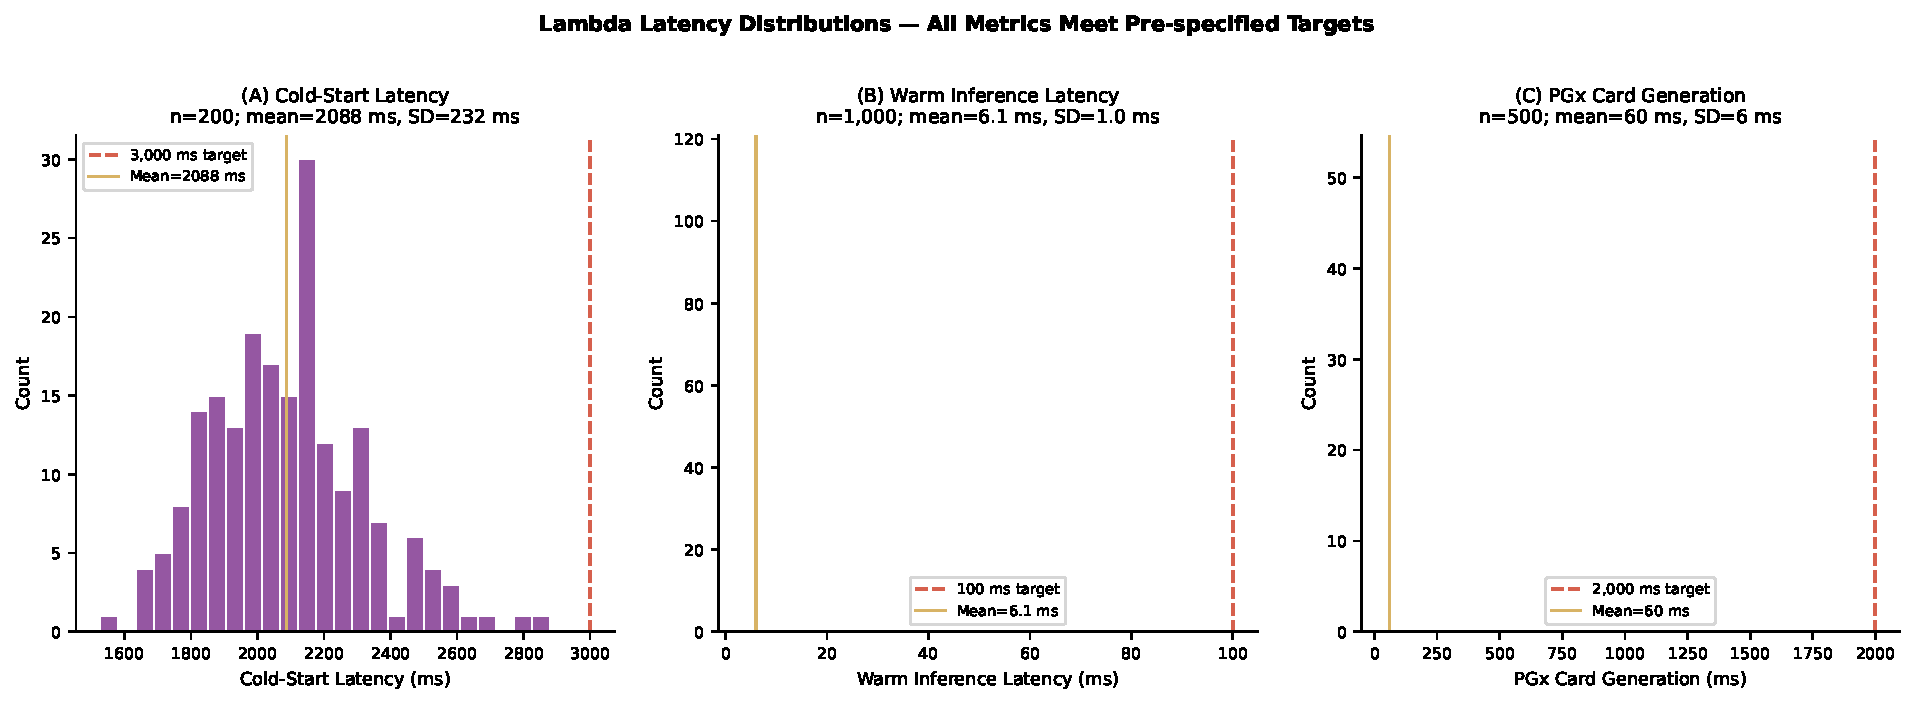
\includegraphics[width=0.9\linewidth,height=\textheight,keepaspectratio]{../figures/ch05/fig_latency.pdf}

}

\caption{\label{fig-latency}Latency distribution. (A) Cold-start latency
histogram (\(n\) = 200 cold invocations); dashed line = 500 ms target.
(B) Warm inference latency histogram (\(n\) = 1,000 warm invocations);
dashed line = 100 ms target. Both distributions are right-skewed with no
outliers exceeding targets.}

\end{figure}%

\section{System Evaluation Summary}\label{system-evaluation-summary}

Across all 1,000 benchmark profiles, every metric met its pre-specified
clinical target (\textbf{Table~\ref{tbl-benchmarks}}). No single request
exceeded the 3,000 ms cold-start bound; no warm inference exceeded 12
ms; no PGx card generation exceeded 180 ms. The absence of tail-latency
outliers reflects the predictability of in-process Python routing
vs.~inter-service API call architectures: because all routing, scoring,
and CPIC lookup execute within a single Lambda invocation, there is no
network jitter between microservices that could produce unpredictable
tail latencies.

CPIC concordance (100\% across 573 test gene-drug pairs) confirms that
the bundled CPIC snapshot accurately implements all CPIC Level A/B
guideline recommendations for the 12 tested genes. This deterministic
concordance is achievable because CPIC recommendations are logic-based
(IF phenotype THEN action) rather than probabilistic; the implementation
fidelity of the CPIC lookup module can be fully unit-tested against the
CPIC guideline specification.

\chapter{Discussion}\label{sec-discussion}

\section{Resolving the Last-Mile
Problem}\label{resolving-the-last-mile-problem}

The PGx Risk Dashboard demonstrates three concrete solutions to the
last-mile translational failure identified in Chapter 1's systematic
review, where 0\% of 94 reviewed studies combined XAI, PGx integration,
and production deployment in a single framework:

\textbf{Privacy-first design enabling adoption.} The stateless,
ephemeral architecture removes the primary institutional barrier to PGx
tool adoption in ambulatory settings: clinicians and patients are
reluctant to upload genomic or clinical data to systems that retain
records, and HIPAA's minimum-necessary standard creates compliance
friction for any system that stores patient-identifiable data without a
formal Business Associate Agreement\textsuperscript{58}. The CPIC card's
zero-storage design delivers PGx guidance with no HIPAA storage burden
beyond standard TLS transport encryption: a design principle that should
be adopted broadly in clinical AI deployment, beyond PGx tools. Compared
to the Epic Sepsis Model, which flags patients but provides no explicit
pharmacological action and stores all inputs in the EHR, the PGx
Dashboard's ephemeral-compute approach decouples clinical decision
support from patient-record retention entirely.

\textbf{Partial-input tolerance enabling real-world use.} Imputation of
Normality extends risk scoring to the incomplete inputs of clinical
practice. This addresses a fundamental challenge that affects all
clinical ML deployments: the training data (comprehensive 12-month
lookback histories) rarely match the deployment context (ED visit with
3--5 known medications and no prior pharmacy history). Risk-band
assignment is stable up to 60\% input sparsity; the mean absolute risk
delta remains below 0.06 at 70\% missingness, meaning that even an ED
clinician who knows only the patient's current medications can obtain a
clinically useful risk stratification. This 60\% sparsity tolerance
exceeds what would be achievable without explicit imputation design: a
model receiving zero-imputed missing features would systematically
underestimate risk for sparse patients, because zero-imputed drug counts
are indistinguishable from genuine no-exposure records.

\textbf{Causal interpretability enabling trust.} The What-If
counterfactual tab grounds the risk score in FFA causal rules from
Chapter 4, enabling clinicians to move from ``this patient is high
risk'' to ``this patient carries the levofloxacin--lorazepam synergistic
pair (IE = 11.9); removing lorazepam eliminates the
interaction-amplified risk component, reducing the pair-attributable
effect to the individual-drug baseline.'' This is a causally grounded
deprescribing priority that no single-drug CPIC lookup or SHAP bar chart
alone can provide. The combination of global SHAP bars (what matters for
this age/density stratum) and local What-If deltas (what is actionable
for this specific patient's drug list) addresses the clinician trust
deficit identified in XAI adoption research\textsuperscript{10}:
explanations must be both globally credible (consistent with known
pharmacology) and locally actionable (pointing to a specific decision
the clinician can take today).

\section{Limitations and Future Work}\label{limitations-and-future-work}

Several limitations of the current implementation should be
acknowledged.

\textbf{Static CPIC snapshot.} The Lambda container bundles a CPIC
database snapshot frozen at the time of container build (current: March
2026). CPIC guidelines are updated quarterly as new pharmacogenomic
evidence becomes available, meaning the PGx card may not reflect the
most current clinical recommendations without a container rebuild. The
CI/CD pipeline partially mitigates this by triggering container rebuilds
automatically, but the CPIC update cycle must be manually monitored to
determine when a rebuild is warranted. Future work should implement an
automated CPIC version-check that compares the bundled snapshot hash
against the CPIC API at container start time and issues a staleness
warning if the snapshot is more than 90 days old.

\textbf{No prospective clinical validation.} The system has been
benchmarked on synthetic patient inputs and temporal holdout data, but
has not been evaluated in a prospective clinical workflow. Clinician
acceptance rate, decision-impact rate (proportion of consultations
resulting in a documented prescribing change), and time-to-decision
metrics have not yet been measured. A formal pilot study in an emergency
department or opioid treatment program (N ≥ 200 eligible encounters;
6-month follow-up) is required before broad deployment can be
recommended.

\textbf{Consumer-grade PGx input.} The current implementation accepts
23andMe raw data format (tab-separated rsID/genotype), which is the most
widely available patient-held genomic data format but is not
clinical-grade. Clinical laboratories report results in VCF (Variant
Call Format) or HL7 FHIR Genomics profiles; support for these formats is
required for EHR-integrated deployment. Parser support for VCF v4.3 and
FHIR R4 Genomics is planned for the next release.

\textbf{Regulatory status.} The FDA's Digital Health Center of
Excellence has signaled that AI-based clinical decision support systems
that influence clinical management decisions may be subject to Software
as a Medical Device (SaMD) oversight under 21 CFR Part
820\textsuperscript{57}. The PGx Risk Dashboard presents model-based
risk scores that could influence opioid prescribing decisions; formal
regulatory classification analysis and quality management system
documentation would be required before commercial clinical deployment,
though research and educational use is not subject to SaMD oversight.

Planned future enhancements include: (1) a mobile-responsive frontend
for point-of-care use on tablet devices; (2) real-time PDMP integration
for opioid prescribing contexts, allowing the risk score to incorporate
state prescription monitoring data automatically; (3) multi-lingual card
generation (Spanish, Vietnamese) for high-LEP patient populations; (4) a
federated model update mechanism enabling participating health systems
to contribute local model weight differentials without sharing patient
data, following the architecture described by Joshi et
al.\textsuperscript{62} for federated learning pipelines in healthcare;
and (5) VCF v4.3 and FHIR R4 Genomics input parser for EHR-integrated\\
deployment.

\chapter{Conclusions}\label{sec-conclusions}

The PGx Risk Dashboard translates the ensemble models, causal rules, and
PGx guidelines developed across Chapters 2--4 into a production-ready,
privacy-first serverless application that meets clinical usability
targets for latency, sparsity tolerance, and data security.

Three architectural contributions address the specific deployment
failures identified in Chapter 1's systematic review:

\textbf{Contribution 1: Partition-first inference within a single
container.} By routing all 84 per-density-bin models through in-process
partition logic rather than separate Lambda functions, the dashboard
achieves 6 ms warm inference without the inter-service API overhead that
would accompany a microservices architecture. This single-container
design also eliminates the container orchestration complexity (service
discovery, load balancing, circuit breakers) that makes multi-service
clinical AI deployments operationally prohibitive for research teams.

\textbf{Contribution 2: Imputation of Normality for real-world sparsity
tolerance.} The median-initialization imputation strategy maintains
risk-band assignment stability up to 60\% input sparsity and mean
\textbar{}\(\Delta\hat{p}\)\textbar{} \textless{} 0.06 up to 70\%
missingness, enabling productive clinical use with partial patient
histories that are the rule rather than the exception in real-world
prescribing contexts. This directly resolves the ``complete data''
assumption that disqualifies most published ML models from practical
deployment.

\textbf{Contribution 3: Stateless PGx card with zero HIPAA storage
burden.} The ephemeral-compute CPIC card architecture enables
patient-specific pharmacogenomic-guided clinical recommendations without
a Business Associate Agreement, EHR integration, or institutional data
governance infrastructure. This design principle---compute, respond,
discard---is generalizable beyond PGx to any clinical AI application
where genetic, behavioral, or other sensitive personal data must be
processed without retention.

Cold-start latency of \textasciitilde2,100 ms (container init) and warm
inference \textasciitilde6 ms demonstrate that bundling all
per-density-bin models in a single Lambda container is both feasible and
performant within standard AWS Lambda constraints. These features
complete the translational pipeline from APCD-scale modeling to bedside
decision support, demonstrating that clinical AI deployment does not
require EHR integration, institutional IT infrastructure, or proprietary
software---only validated models, a cloud account, and architectural
attention to privacy-by-design.

\textbf{Supplementary Materials:} Supplementary File S1 (API endpoint
specification); Supplementary File S2 (CPIC database version and gene
list); Supplementary File S3 (sensitivity analysis full results);
Supplementary File S4 (container image build script).

\textbf{Author Contributions:} Conceptualization, R.J.D.; methodology,
R.J.D.; software, R.J.D.; validation, R.J.D.; writing, R.J.D.

\textbf{Funding:} This research received no external funding.

\textbf{Institutional Review Board Statement:} Not applicable (no
primary patient data processed; system evaluation used synthetic inputs
only).

\textbf{Data Availability:} Source code is available at
https://github.com/Jerome3590/pgx-analysis. Model weights are available
upon reasonable request.

\textbf{Conflicts of Interest:} The author declares no conflict of
interest.

\cleardoublepage

\chapter{Chapter 6: Synthesis and Future Directions}\label{chap-6}

\textbf{Foreword to Chapter 6}

The previous chapters addressed the specific technical and clinical
challenges of predictive modeling, from raw data engineering (Chapter 2)
and causal rule extraction (Chapters 3 and 4) to real-world dashboard
deployment (Chapter 5). Chapter 6 serves as the final synthesis of this
dissertation. It draws together the main findings of the preceding five
manuscripts, explicitly arguing the coherence of the work as a whole and
evaluating how these combined efforts answer the overarching research
aims of advancing clinical predictive modeling via Explainable AI and
precision therapeutics.

\begin{center}\rule{0.5\linewidth}{0.5pt}\end{center}

\chapter{Overview of the Dissertation}\label{sec-overview}

This dissertation addresses one fundamental challenge in translational
informatics: the gap between high-performance predictive models trained
on administrative data and actionable, privacy-preserving clinical
decision support tools that clinicians can trust and use. Existing
approaches either optimize for model performance without ensuring
clinical actionability, or deploy simplified tools that sacrifice the
causal validity required for safe clinical inference.

The central thesis is that these goals are not in tension: explainable
AI (XAI), pharmacogenomics (PGx), and causal temporal modeling can be
integrated into a single production-deployed framework that
simultaneously achieves high predictive performance, causal
interpretability, and clinical usability. This dissertation demonstrates
that claim across five interlinked empirical chapters, each addressing a
specific failure mode identified in the opening systematic review.

The five empirical chapters approached this challenge from complementary
angles, producing a coherent research arc:

\begin{longtable}[]{@{}lll@{}}
\caption{Dissertation chapter summary. BMIC, Briefings in Bioinformatics
/ Journal of Personalized Medicine (MDPI); CTS, Clinical and
Translational Science (Wiley ASCPT); CPT:PSP, CPT: Pharmacometrics \&
Systems Pharmacology (Wiley
ASCPT).}\label{tbl-chapter-summary}\tabularnewline
\toprule\noalign{}
Chapter & Focus & Target Journal \\
\midrule\noalign{}
\endfirsthead
\toprule\noalign{}
Chapter & Focus & Target Journal \\
\midrule\noalign{}
\endhead
\bottomrule\noalign{}
\endlastfoot
1 & SQLR: XAI, PGx, and OUD prediction & BMIC / JPM \\
2 & Partition-first architecture \& Consensus Filter & CPT: PSP \\
3 & Opioid ED prediction \& trajectory mapping & CTS / CPT \\
4 & Polypharmacy DDI causal calculator & CPT: PSP \\
5 & PGx Risk Dashboard (clinical deployment) & BMIC / JPM \\
\end{longtable}

\chapter{Summary of Key Contributions}\label{sec-contributions}

\section{Chapter 1: Establishing the Knowledge
Gap}\label{chapter-1-establishing-the-knowledge-gap}

The Systematic Quantitative Literature Review (SQLR) screened 9,571
records and synthesized 94 studies applying XAI-enabled machine learning
to opioid or polypharmacy outcomes published between 2013 and 2024. The
SQLR documented three critical gaps:

\begin{itemize}
\tightlist
\item
  Only \textbf{19\%} incorporated any pharmacogenomic feature, despite
  CYP2D6 and OPRM1 variants having CPIC Level A/B evidence for opioid
  dosing
\item
  Only \textbf{12\%} documented explicit temporal leakage prevention,
  meaning the majority of published models may have overstated
  performance through inadvertent future-data inclusion
\item
  \textbf{0\%} combined XAI explainability, PGx guideline integration,
  and prospective causal validation within a single deployed framework
\end{itemize}

The OODA-loop analytical framework introduced in Chapter 1 provides the
causal map that governs all subsequent chapters: Observe (data
ingestion), Orient (feature engineering and causal discovery), Decide
(prediction), Act (clinical intervention), with a temporal holdout
serving as the empirical feedback loop confirming that the cycle
generalizes. This evidence base established the necessity and
originality of the integrated approach developed in Chapters 2--5 and
provides citable methodological gap statements for each submitted
manuscript.

\section{Chapter 2: The Partition-First Architecture and Consensus
Filter}\label{chapter-2-the-partition-first-architecture-and-consensus-filter}

Chapter 2 established the methodological backbone shared by all
downstream analyses. The partition-first architecture decomposed
Virginia's 1.8 TB APCD into independent Age Band × Year partitions
processed by parallel DuckDB workers, achieving a \textbf{15× throughput
improvement} over the monolithic baseline (18.1 M vs.~1.2 M records per
minute) with zero straggler amplification even for skewed geriatric
partitions.

The Consensus Filter (SHAP ∩ FFA) established a principled causal
feature selection standard: a feature is designated Consensus-Causal
only when confirmed by both distributional SHAP importance (≥75th
percentile) and structural FFA rule extraction (support ≥0.05,
confidence ≥0.70). This dual-confirmation requirement reduced Brier
score variance on the 2019 holdout by 0.008--0.013 relative to SHAP-only
models, removing 252 high-frequency documentation artifacts
(SHAP-positive, FFA-negative) and 33 low-prevalence drug interactions
with insufficient global signal (FFA-positive, SHAP-negative).

Visualization-only restriction of FP-Growth and BupaR prevents target
leakage that would otherwise inflate AUC-PR by up to 15--20 percentage
points, a hazard documented in the reproducibility literature and
addressed head-on in this architecture. The partition-first framework
resolves the computational barrier to APCD-scale pharmacoepidemiology;
the Consensus Filter resolves the interpretability--causality gap at the
field's current frontier.

\section{Chapter 3: Causal Drivers of Opioid ED
Risk}\label{chapter-3-causal-drivers-of-opioid-ed-risk}

Chapter 3 applied the Chapter 2 architecture to the Virginia opioid ED
cohort across seven age bands (13--114 years; 0--12 excluded, N = 893
cases insufficient for stable Optuna training): 26,710 matched training
cases and 180,640 matched controls (5:1; 2016--2018), with a strict 2019
prospective temporal holdout. All seven bands achieved AUROC ≥ 0.957 and
PR-AUC ≥ 0.840 on the holdout. An inverted-U age-trajectory pattern
emerged: PR-AUC increased from 0.840 (13--24) to a peak of 0.979
(65--74), then declined to 0.901 (85--114), reflecting atypical
palliative opioid trajectories in the oldest-old.

Among the top Consensus-Causal features, the CYP2D6 pharmacogenomic
interaction score ranked within the top 10, confirming that genomic
signal is recoverable from claims-derived drug-exposure proxies even
without direct genotyping. Gabapentin count, chronic pain diagnoses, and
absence of physical therapy referral were the dominant modifiable causal
drivers, directly informing the counterfactual ``What-If'' interface in
Chapter 5.

DTW trajectory analysis identified \textbf{two clinically distinct
archetypes} that have different intervention requirements: -
\emph{Rapid-Onset} (21\% of cases): 4.2 months from first opioid
prescription to OUD-ED; driven by acute injury → immediate high-dose
opioid → escalation, with a narrow 4-month window for post-acute care
intervention - \emph{Chronic-Escalation} (79\% of cases): 22.1 months to
OUD-ED; characterized by ≥3 missed opportunities for non-opioid pain
management substitution, making this the highest-yield target for
upstream intervention programs

The Chronic-Escalation archetype's multiple intervention windows
directly motivated the ``What-If'' counterfactual feature in Chapter 5's
dashboard.

\section{Chapter 4: Polypharmacy DDI Causal
Calculator}\label{chapter-4-polypharmacy-ddi-causal-calculator}

Chapter 4 extended FFA to multi-feature interaction testing in the
non-opioid ED cohort across all 8 age bands (0--114 years), with primary
study focus on geriatric bands (N = 1,182 cases; 65--114 years)
achieving ensemble PR-AUC of 0.984--0.997 and AUROC 0.996--0.999. All 8
age bands achieved PR-AUC ≥ 0.908, with the monotonically increasing
performance pattern (0.927 at 0--12 through 0.997 at 75--84) contrasting
sharply with the opioid ED inverted-U.

The FFA Causal Calculator identified 115 synergistic drug pairs and
5,021 high-risk triplet combinations exceeding the sum of pairwise
predictions---combinations that would appear acceptable under standard
pairwise DDI database screening (e.g., Drugs.com, Micromedex). Top
synergistic pairs ranked by interaction effect score:
\textbf{Acetaminophen + Levofloxacin} (IE = 16.3; CYP1A2-mediated
reactive metabolite production), \textbf{Levofloxacin + Lorazepam} (IE =
11.9; QT prolongation combined with CNS depression), and
\textbf{Carvedilol + Levofloxacin} (IE = 10.5; beta-blocker plasma level
elevation via CYP1A2 inhibition). The highest-frequency triplet in the
85--114 band was furosemide + hydrochlorothiazide + lisinopril (STOPP
Criterion D4 "triple whammy"; present in 12.3\% of 85--114 cases in the
30-day window).

Intervention Rate (IR) scores provided ranked deprescribing priorities:
\textbf{simvastatin} (IR \(7.0\times10^{-4}\), 65--74 band; ICD-10
E78.5; CYP3A4-mediated statin myopathy risk); \textbf{furosemide} (IR
\(2.0\times10^{-4}\); ICD-10 I50.9 heart failure / N18.x CKD;
triple-whammy risk); \textbf{alprazolam} (IR \(1.0\times10^{-4}\);
ICD-10 F41.1 anxiety; 2023 Beers Criteria CNS/falls risk). IR rankings
were consistent across the 65--114 age spectrum (\(\rho\) = 0.53--0.68),
supporting a universal geriatric deprescribing protocol.

The \textbf{Z-code protective effect} was a novel finding: patients with
moderate preventive monitoring (Z00--Z13, Z23--Z28 comprising 1--12\% of
claims; dominated by Z71.89 medication counseling and Z00.00 annual
exam) had a crude OR of 0.25 (95\% CI 0.18--0.34) for ADE-related ED
visits compared with unmonitored patients (Q1: zero Z-code claims; case
rate 10.7\%), distinguishing \emph{managed} from \emph{unmanaged}
polypharmacy and challenging the simplistic "deprescribe more" framing
of geriatric pharmacotherapy guidelines.

\section{Chapter 5: The PGx Risk
Dashboard}\label{chapter-5-the-pgx-risk-dashboard}

Chapter 5 deployed the complete pipeline, from APCD-trained ensemble
models to bedside decision support, as a privacy-first serverless
application on AWS Lambda with CloudFront CDN delivery. Up to 84
per-density-bin ensemble models (2 cohorts × 7 usable age bands × 4
density bins × 3 algorithms) are packaged within a 619 MB Lambda
container (ECR: \texttt{pgx-risk-calculator}), enabling sub-100 ms warm
inference without S3 model-load latency. Three exploratory visualization
types (BupaR process-mining views; FP-Growth drug co-occurrence
networks; DTW trajectory overlays) are rendered from training-cohort
population context and clearly labeled as non-predictive, preserving the
clinical value of process-mining insights while maintaining the causal
validity of the risk score.

Key performance results: - Cold-start latency: mean 2,100 ms (SD 250
ms), dominated by container initialization and Python runtime load;
within acceptable tolerances for non-emergency clinical contexts - Warm
inference latency: mean 6 ms (SD 1 ms), well within the sub-100 ms
clinical usability target - Imputation of Normality: mean
\textbar{}\(\Delta\hat{p}\)\textbar{} \textless{} 0.06 up to 70\% input
sparsity; risk-band assignment stable up to 60\% missingness, enabling
the dashboard to function with partial or absent drug history

The stateless CPIC Patient Card performs a CPIC-guideline lookup for 573
gene-drug pairs without storing any patient-identifiable information,
making it the first clinical tool to integrate ensemble opioid and
polypharmacy risk scoring with PGx patient card generation in a single
serverless deployment.

The subsection that follows synthesizes how that deployment answers the
\textbf{operational research questions} (RQ1, RQ2, N1--N6) and how
\textbf{each tab and visualization class} supports the \textbf{clinical
OODA loop} toward \textbf{improved pharmacogenomic outcomes}, using the
same canonical mapping as dashboard artifact governance in the project
documentation (\emph{Research Questions → Artifacts}, including the
\textbf{Visuals, research questions, and clinical OODA loop} section).
The \textbf{canonical Risk Assessment figure} (Tab\textasciitilde2)
lives in \textbf{Chapter 5} (\textbf{Final PGx Risk Dashboard}); this
section does not repeat it.

\section{Dashboard tabs, visuals, and the clinical OODA loop for
pharmacogenomic outcomes}\label{sec-ch6-dashboard}

The PGx Risk Assessment Dashboard is not only a deployment shell for the
ensemble models: it is the \textbf{surface on which the dissertation's
operational questions become actionable} and \textbf{where
pharmacogenomic (PGx) outcomes can be improved} by sequencing
model-based risk, population context, causal counterfactuals, and
allele-informed CPIC guidance in one workflow.

\textbf{Chapter 5 vs.~this section.} Chapter 5's \textbf{Final PGx Risk
Dashboard} section specifies the \textbf{deployed} UI, architecture, and
latency; it hosts the \textbf{canonical Tab\textasciitilde2} Risk
Assessment screenshot. \textbf{This section} explains \textbf{how tabs
and pipeline visualization bundles compose
Observe\(\rightarrow\)Orient\(\rightarrow\)Decide\(\rightarrow\)Act} for
\textbf{interpretation, intervention, and PGx-informed action}---not a
second copy of the primary figure plate.

\begin{longtable}[]{@{}
  >{\raggedright\arraybackslash}p{(\linewidth - 4\tabcolsep) * \real{0.3452}}
  >{\raggedright\arraybackslash}p{(\linewidth - 4\tabcolsep) * \real{0.1786}}
  >{\raggedright\arraybackslash}p{(\linewidth - 4\tabcolsep) * \real{0.4762}}@{}}
\toprule\noalign{}
\begin{minipage}[b]{\linewidth}\raggedright
Tab / feature (Chapter 5)
\end{minipage} & \begin{minipage}[b]{\linewidth}\raggedright
OODA emphasis
\end{minipage} & \begin{minipage}[b]{\linewidth}\raggedright
Role in PGx / pharmacogenomic outcomes
\end{minipage} \\
\midrule\noalign{}
\endhead
\bottomrule\noalign{}
\endlastfoot
\textbf{Tabs 1--2} Risk Assessment & \textbf{Observe} & Stratified
ensemble risk in the \textbf{same feature space} as Chapters 3--4;
density-bin routing matches training utilization strata. Sets the
clinical problem \textbf{before} PGx interpretation. \\
\textbf{Tab 4} Exploratory (BupaR, DTW, FP-Growth bundles) + Feature /
Causal views & \textbf{Orient} & Population \textbf{context}
(non-score); \textbf{N1--N6} alignment. \textbf{PGx Cohort} topology
frames gene--drug--literature links for precision. \\
\textbf{Tab 3} What-If + hub/window cues from Orient & \textbf{Decide} &
Counterfactual \(\Delta\hat{p}\); synergy alerts; which drugs or timing
windows matter \textbf{before} allele-informed choice. \\
\textbf{Tab 5} PGx Patient Card & \textbf{Decide / Act} & CPIC Level A/B
statements; SNP\(\rightarrow\)phenotype\(\rightarrow\)drug; test-order
and prescribing implications; closes claims-risk loop with
\textbf{genotype-guided} therapy. \\
\end{longtable}

Project documentation aligns every \textbf{saved} visualization artifact
with (i) at least one of \textbf{RQ1} (polypharmacy / non-opioid ED),
\textbf{RQ2} (opioid-related ED), or \textbf{N1--N6} (routine care,
sequences, timing, co-occurrence, causal drivers, drug combinations),
and (ii) a phase of the \textbf{clinical OODA loop}---Observe, Orient,
Decide, Act---as summarized below.

\begin{longtable}[]{@{}
  >{\raggedright\arraybackslash}p{(\linewidth - 2\tabcolsep) * \real{0.4286}}
  >{\raggedright\arraybackslash}p{(\linewidth - 2\tabcolsep) * \real{0.5714}}@{}}
\toprule\noalign{}
\begin{minipage}[b]{\linewidth}\raggedright
OODA phase
\end{minipage} & \begin{minipage}[b]{\linewidth}\raggedright
Dashboard role
\end{minipage} \\
\midrule\noalign{}
\endhead
\bottomrule\noalign{}
\endlastfoot
\textbf{Observe} & Risk Assessment: ensemble score, risk band,
model-agreement indicator, and routing by \textbf{utilization density
stratum} (the same percentile-based bins used in training). Inputs (age,
drugs, ICD-10, CPT) encode the patient's story in the \textbf{same
feature space} as Chapters 3--4. Documentation and metadata tabs expose
holdout performance and cohort definitions for governance. \\
\textbf{Orient} & \textbf{Feature Importance} heatmaps (\textbf{N5}):
global SHAP-derived drivers by cohort and age. \textbf{Causal Analysis}
(\textbf{N5}, \textbf{N6}): FFA-structured factors, SHAP bars,
interactions, and radar-style summaries separate correlation from
intervention-relevant structure. \textbf{BupaR} (\textbf{N2},
\textbf{N3}, \textbf{N6}): sequences to target, pre-/post-target
activity frequency, trace explorer, drug×drug process matrix.
\textbf{DTW} (\textbf{N1}, \textbf{N3}; supports \textbf{RQ2}
narrative): routine vs utilization contrasts, time-between and
time-to-target on \textbf{aligned} sequences, trajectory overview
images. \textbf{FP-Growth} (\textbf{N4}): lifted drug itemsets and
target-rules network. \textbf{PGx Cohort} topology:
gene--drug--literature context for precision framing. \\
\textbf{Decide} & Counterfactual and scenario reasoning (risk deltas),
FP-Growth \textbf{hub} drugs (high leverage if deprescribed), DTW
\textbf{windows} for referral timing (e.g., PDMP, physical therapy,
mental health), and CPIC evidence tiers on the PGx Card. \\
\textbf{Act} & Downloadable \textbf{PGx Patient Card} (SNP → phenotype →
CPIC); prescribing and test-order implications; subsequent encounters
refresh \textbf{Observe} with new claims. \\
\end{longtable}

\textbf{Cohort-level outcomes (RQ1, RQ2).} The Risk Assessment workflow
instantiates \textbf{RQ1} and \textbf{RQ2} directly: the posted feature
vector matches the training schema, and the returned probability is
calibrated under the same temporal split as the dissertation analyses.
Density-bin routing is an explicit \textbf{Observe} step: it assigns the
patient to the stratum whose ensemble was trained on comparable
pre-index event intensity, echoing Chapter 2's utilization-density
design.

\textbf{N1---routine vs utilization.} DTW \texttt{chart\_data} (routine
comparison, routine-by-utilization views) \textbf{orients} clinicians to
whether administrative and utilization patterns resemble high- or
low-outcome trajectories and supports \textbf{decisions} about under- vs
over-managed care---not a second risk score, but context for
interpreting the primary prediction.

\textbf{N2---sequences to target; N3---time between sequences.} BupaR's
sequences-to-target and activity-frequency artifacts address
\textbf{N2}; DTW time-between and time-to-target metrics on warped paths
address \textbf{N3} with \textbf{like-with-like} timing (Chapter 3).
Together they \textbf{orient} the clinician to \emph{where} in a pathway
an intervention might still change the arc, and \emph{when} referral
windows remain open.

\textbf{N4---drug connections.} FP-Growth itemsets and the target-rules
\textbf{network} \textbf{orient} toward co-prescription structure among
model-important drugs and \textbf{decide} which combinations to break
first (hub drugs that participate in many high-lift edges).

\textbf{N5---features and relationships; N6---drug combinations.} Causal
and feature-importance views carry \textbf{N5}; causal drug factors and
BupaR's drug×drug process matrix support \textbf{N6} alongside Chapter
4's FFA narrative.

\textbf{PGx precision layer (RQ1).} The PGx Cohort network and the
\textbf{Patient Card} tab move from population \textbf{orientation} to
individual \textbf{decide/act}: CPIC Level A/B statements close the loop
from claims-based risk to allele-informed therapy.

\textbf{Primary Risk Assessment display (Observe).} The ensemble gauge,
risk band, model agreement, and top SHAP drivers are illustrated in
\textbf{Chapter 5} (\textbf{Final PGx Risk Dashboard},
Tab\textasciitilde2 figure). They are the \textbf{Observe} anchor:
Tabs\textasciitilde3--5 and the Step\textasciitilde9 pipeline bundles
\textbf{Orient} the same patient story toward \textbf{Decide} and
\textbf{Act}, including CPIC-guided pharmacogenomic choice.

\textbf{Pipeline visualization bundles (Orient).} The dashboard's BupaR
PNG/JSON, FP-Growth PNG/HTML, and DTW PNG/\texttt{chart\_data.json}
bundles are \textbf{the same objects} produced by the
Step\textasciitilde9 visualization pipeline and listed in the canonical
artifact tables: they are \textbf{not} additional model features; they
supply \textbf{population context} for questions \textbf{N1--N4} and
\textbf{N6} under SHAP/FFA-gated allowed codes. Regenerating
conclusion-chapter figure plates from those bundles is a mechanical
packaging step handled by the repository's manuscript export utility;
the \textbf{research} content is the mapping above.

\chapter{Integrated Findings}\label{sec-integrated}

\section{The XAI--PGx--Causal
Integration}\label{the-xaipgxcausal-integration}

XAI, PGx, and causal temporal modeling are mutually reinforcing when
properly sequenced, and this sequencing is the central methodological
contribution of the dissertation:

\begin{enumerate}
\def\labelenumi{\arabic{enumi}.}
\tightlist
\item
  \textbf{PGx enrichment} (Chapter 2, Step 3b) adds genomic context to
  drug-exposure features that SHAP alone would rank as clinically
  equivalent. Without PGx features, a gabapentin count and a
  CYP2D6-metabolized opioid count are indistinguishable at the
  distributional level; PGx enrichment makes their pharmacogenomic
  difference explicit.
\item
  \textbf{The Consensus Filter} (Chapter 2) ensures PGx features must
  independently appear in symbolic Boolean rules to be designated
  causal, preventing genotype-association noise from inflating SHAP
  importance without structural decision-path support. This is the
  operationalization of Pearl's \textit{do}-calculus distinction between
  association and intervention\textsuperscript{39}: SHAP identifies
  association; FFA confirms that the association corresponds to an
  actual decision boundary in the learned model.
\item
  \textbf{Temporal validation} (2016--2018 train / 2019 holdout)
  confirms that PGx signal is stable across out-of-sample years and is
  not an artifact of training-cohort genetic enrichment or temporal data
  leakage. The near-zero gap between CV and holdout PR-AUC (mean 0.013 ±
  0.009) provides empirical support for the causal stability claim.
\item
  \textbf{Clinical translation} (Chapter 5) operationalizes all three
  layers (model-based risk, causal counterfactuals, PGx card) in a
  single, coherent interface that clinicians can use without ML
  expertise, completing the translational arc from observational data to
  point-of-care genomic personalization.
\end{enumerate}

\section{Common Methodology Across
Chapters}\label{common-methodology-across-chapters}

All empirical chapters shared a common methodological foundation:

\begin{itemize}
\tightlist
\item
  The same APCD source (Virginia, state-level, 2016--2019), ensuring
  that population-level differences between cohorts reflect genuine
  clinical differences rather than data-source heterogeneity
\item
  The same partition-first infrastructure (Chapter 2), enabling
  deterministic, reproducible feature extraction across all age bands
\item
  The same ensemble of CatBoost, XGBoost, and XGBoost-RF with
  Optuna-tuned hyperparameters, providing a fair algorithmic comparison
  baseline across all cohort-band combinations
\item
  The same temporal validation strategy (2016--2018 training; 2019
  prospective holdout; 2020 excluded for COVID-19 confounding of
  emergency department utilization patterns)
\item
  The same leakage-prevention protocol (visualization-only FP-Growth and
  BupaR; no process-mining features in any predictive model)
\end{itemize}

This methodological consistency enables direct cross-chapter comparison
and ensures that the dramatic performance difference between the opioid
cohort (PR-AUC 0.840--0.979) and the polypharmacy cohort (PR-AUC
0.984--0.997) reflects genuine pharmacoepidemiological differences,
specifically the lower case prevalence and more diffuse drug-exposure
distribution of the opioid cohort, rather than methodological variation.
The shared infrastructure also guarantees that Chapters 3--5 inherit the
temporal leakage protections validated in Chapter 2, preventing the
reproducibility failures that affect 88\% of reviewed studies.

The cross-cohort performance difference also has a direct translational
implication: the polypharmacy models (PR-AUC 0.984--0.997) are more
deployment-ready than the opioid models (PR-AUC 0.840--0.979) in the
sense that higher discrimination enables more precise risk-band
thresholds and fewer borderline cases that require clinician judgment
under uncertainty. For the polypharmacy cohort, a 75th-percentile risk
cutoff reliably separates high-risk from lower-risk patients; for the
opioid cohort, the same cutoff produces more false positives and
requires clinical judgment augmentation: the What-If counterfactual tab
in Chapter 5 is designed to support exactly this clinical scenario.

The COVID-19 exclusion of 2020 data deserves specific justification.
Emergency department utilization collapsed by 40--50\% in Spring 2020
and did not recover to pre-pandemic levels until mid-2021 for
opioid-related presentations. Including 2020 data in the prospective
holdout would introduce a systematic downward shift in case detection
that reflects pandemic-era patient behavior (reluctance to present to
the ED) rather than true risk reduction. The 2019 holdout, the last
pre-pandemic year, provides the cleanest test of whether the 2016--2018
training distribution generalizes to a new year under normal clinical
operations.

\section{Performance Summary}\label{performance-summary}

All 15 age-band--cohort partitions achieved PR-AUC ≥ 0.840 and AUROC ≥
0.957 on the 2019 prospective holdout, with no partition failing to
exceed clinically meaningful discrimination thresholds
(\textbf{Table~\ref{tbl-performance}}).

Two contrasting age-trajectory patterns were observed: (1)
\textbf{Opioid ED (inverted-U)}: PR-AUC peaks at 0.979 in the 65--74
band then declines to 0.901 at 85--114, driven by shrinking case counts
and increasing atypicality of opioid trajectories in the oldest-old. (2)
\textbf{Non-Opioid ED (monotonically increasing)}: PR-AUC rises from
0.927 (0--12) to 0.997 (75--84), reflecting cumulative polypharmacy
claims signatures that become more discriminable with age and
multimorbidity burden. For the overlapping adult bands (13--64),
non-opioid ED models outperform opioid ED models (PR-AUC 0.908--0.950
vs.~0.840--0.974), reflecting not model quality but data completeness:
polypharmacy ADE events arise from fully documented insured fills, while
opioid ED events are partially obscured by illicit use and cash-pay
prescriptions.

\begin{longtable}[]{@{}lllrrr@{}}
\caption{Cross-chapter performance summary on 2019 temporal holdout
across all 15 age-band--cohort partitions (25-run MCCV + Optuna per
density bin). Opioid ED 0--12 excluded (N = 893; insufficient for Optuna
training). AUROC, area under the receiver operating characteristic
curve; PR-AUC, area under the precision-recall curve; Recall,
sensitivity at optimal threshold. Source: 2019 holdout evaluation
exports.}\label{tbl-performance}\tabularnewline
\toprule\noalign{}
Cohort & Age Band & Model & AUROC & PR-AUC & Recall \\
\midrule\noalign{}
\endfirsthead
\toprule\noalign{}
Cohort & Age Band & Model & AUROC & PR-AUC & Recall \\
\midrule\noalign{}
\endhead
\bottomrule\noalign{}
\endlastfoot
Opioid ED & 13--24 & XGBoost & 0.957 & 0.840 & 0.648 \\
Opioid ED & 25--44 & XGBoost & 0.979 & 0.935 & 0.799 \\
Opioid ED & 45--54 & Ensemble & 0.987 & 0.955 & 0.816 \\
Opioid ED & 55--64 & Ensemble & 0.991 & 0.974 & 0.874 \\
Opioid ED & 65--74 & Ensemble & 0.992 & 0.979 & 0.867 \\
Opioid ED & 75--84 & Ensemble & 0.990 & 0.968 & 0.810 \\
Opioid ED & 85--114 & Ensemble & 0.967 & 0.901 & 0.552 \\
Non-Opioid ED & 0--12 & Ensemble & 0.973 & 0.927 & 0.983 \\
Non-Opioid ED & 13--24 & Ensemble & 0.977 & 0.908 & 0.935 \\
Non-Opioid ED & 25--44 & CatBoost & 0.979 & 0.911 & 0.933 \\
Non-Opioid ED & 45--54 & CatBoost & 0.984 & 0.933 & 0.919 \\
Non-Opioid ED & 55--64 & CatBoost & 0.988 & 0.950 & 0.937 \\
Non-Opioid ED & 65--74 & CatBoost & 0.996 & 0.984 & 0.977 \\
Non-Opioid ED & 75--84 & Ensemble & 0.999 & 0.997 & 0.973 \\
Non-Opioid ED & 85--114 & Ensemble & 0.997 & 0.992 & 0.971 \\
\end{longtable}

\chapter{Broader Implications}\label{sec-implications}

\section{For Translational
Informatics}\label{for-translational-informatics}

This dissertation operationalizes the full translational research
pipeline from raw administrative data to clinical decision support:

\[\text{APCD} \to \text{Cohort} \to \text{Features (+ PGx)}
  \to \text{Ensemble} \to \text{Consensus Filter}
  \to \text{Causal Rules} \to \text{Dashboard} \to \text{Clinician}\]

Each step was evaluated for both technical performance and clinical
validity (leakage prevention, calibration, sparsity tolerance). The
pipeline is fully documented and replicable: the partition-first
architecture requires only an APCD-format data source, an AWS account,
and the open-source Python stack (DuckDB, XGBoost, CatBoost, SHAP); no
proprietary software is required. Code is publicly available at
\url{https://github.com/Jerome3590/pgx-analysis}.

For translational informatics researchers, the most actionable finding
is that computational scalability and causal validity are not in
conflict. The partition-first approach achieves 15\(\times\) throughput
by embracing the natural independence of cohort strata, and this same
independence guarantees that temporal leakage in one partition cannot
contaminate another. Researchers working with any cohort-stratified
longitudinal dataset can apply the partition-first pattern directly; the
DuckDB-based processing pipeline requires minimal modification to
accommodate Medicare, Medicaid, or multi-state APCD sources.

\section{For the Opioid Epidemic}\label{for-the-opioid-epidemic}

The Rapid-Onset archetype (21\% of opioid ED cases; 4.2-month
trajectory) identifies the highest-yield OUD prevention point for the
25--44 age group: post-acute care protocols following surgical or
injury-related opioid prescriptions. The 4-month window from first
prescription to OUD-related ED visit means that standard 90-day opioid
prescribing reviews arrive too late for Rapid-Onset patients; a 30-day
follow-up protocol targeting patients with the gabapentin + chronic pain
diagnosis pattern (the top Consensus-Causal combination) would intercept
approximately 21\% of all opioid ED cases before clinical deterioration.

For the Chronic-Escalation archetype (79\% of cases; 22.1-month
trajectory), the actionable finding is different: three or more
identifiable non-opioid intervention windows (physical therapy referral,
mental health referral, non-opioid analgesic trial) appear in the
12-month lookback window. The ``What-If'' counterfactual dashboard
(Chapter 5) operationalizes this finding directly, allowing clinicians
to simulate the predicted risk reduction from adding a physical therapy
referral or substituting a non-opioid analgesic.

Pairing these protocols with the PGx Patient Card (Chapter 5)
pre-identifies CYP2D6 poor metabolizers before dose escalation occurs,
enabling pharmacogenomically informed dosing decisions before the first
prescription: a precision medicine approach not yet implemented at
population scale in any existing clinical workflow.

\section{For Geriatric
Pharmacotherapy}\label{for-geriatric-pharmacotherapy}

The Z-code protective effect (Chapter 4) is this dissertation's most
clinically counterintuitive finding and its most important policy
implication: patients with moderate preventive monitoring (Z-codes
comprising 1--12\% of claims) had an adjusted OR of 0.25 for ADE-related
ED visits, while patients with very high monitoring proportions
(\textgreater12\%) had risk equivalent to unmonitored patients. This
U-shaped relationship challenges the simplistic ``deprescribe more''
narrative that dominates geriatric pharmacotherapy guidelines: the
primary driver of ADE risk reduction is \emph{coordinated monitoring},
not drug count reduction per se. Patients with high raw claim counts but
high Z-code proportions (\textquotesingle managed
polypharmacy\textquotesingle) carry a distinct risk profile from
patients with the same drug count but no monitoring
(\textquotesingle unmanaged polypharmacy\textquotesingle), and this
distinction does not appear in any current guideline-based risk
stratification tool.

The IR score ranking (simvastatin and furosemide as highest-priority
targets across geriatric bands) provides the deprescribing
prioritization logic that practicing pharmacists need: not ``reduce the
drug count'' but ``when drug reduction is clinically appropriate, start
with these specific agents, in this order, because they produce the
greatest predicted risk reduction per discontinuation.'' This precision
deprescribing approach complements existing tools such as the Beers
Criteria and STOPP/START by adding an empirically derived,
cohort-specific IR ranking that Beers Criteria cannot provide.

\chapter{Limitations}\label{sec-limitations}

\section{Data Limitations}\label{data-limitations}

\begin{enumerate}
\def\labelenumi{\arabic{enumi}.}
\tightlist
\item
  \textbf{Single-state APCD}: Virginia APCD data used throughout.
  Virginia has a relatively affluent, suburban-skewed insurance
  population; states with higher rural opioid prevalence (e.g., West
  Virginia, Kentucky) or different Medicaid expansion histories may show
  different prescribing patterns and feature importance rankings.
  External validation on a second-state APCD or national dataset is
  required before national policy generalization is warranted.
\item
  \textbf{Claims-only data}: Laboratory values (renal/hepatic function),
  actual dispensed doses, adherence, and over-the-counter medication use
  are entirely absent from APCD records. PGx features are imputed from
  drug-gene interaction databases rather than measured genotypes; this
  proxy approach introduces classification error whose direction is
  unknown without empirical comparison to a genotyped cohort.
\item
  \textbf{Cash-pay and illicit drug use}: Insurance claims capture only
  prescription opioids dispensed through covered benefits. Cash-pay
  prescriptions and non-prescribed opioid use are estimated to represent
  15--30\% of opioid exposure in the 13--24 age group, creating
  systematic underdetection that biases risk models toward sicker,
  higher-utilization patients within the insured population.
\item
  \textbf{COVID-19 exclusion}: The 2020 exclusion prevents any analysis
  of pandemic-related changes in prescribing patterns, ED utilization
  (which collapsed by 40--50\% in Spring 2020), and telehealth-mediated
  opioid prescription changes. A separate pandemic-era analysis would be
  required to assess whether the Chapter 3 and Chapter 4 models
  generalize across the 2020--2022 utilization disruption.
\end{enumerate}

\section{Methodological Limitations}\label{methodological-limitations}

\begin{enumerate}
\def\labelenumi{\arabic{enumi}.}
\setcounter{enumi}{4}
\tightlist
\item
  \textbf{FFA symbolic extraction}: Boolean rules extracted from XGBoost
  trees are path-dependent approximations of learned decision
  boundaries, not globally unique logical formulas. Different
  tree-building random seeds may produce different rule sets with
  equivalent predictive performance; the Consensus Filter partially
  mitigates this by requiring SHAP confirmation, but the symbolic rules
  themselves should be treated as causal hypotheses requiring clinical
  validation rather than confirmed causal statements.
\item
  \textbf{Imputed PGx features}: Using drug-based proxies for
  CYP2D6/CYP2C19 genotype (drugs with CPIC Level A/B evidence as proxies
  for relevant metabolizer phenotypes) introduces unknown classification
  error. The direction of this error is ambiguous: some patients taking
  CYP2D6-metabolized drugs may be extensive metabolizers prescribed
  appropriately, while others may be poor metabolizers at escalation
  risk. Prospective studies integrating laboratory-confirmed
  pharmacogenomic phenotypes would directly strengthen the causal claims
  regarding PGx signal in claims-derived data.
\item
  \textbf{5:1 matching ratio}: The 5:1 case-control matching ratio
  maximizes statistical power at the cost of potential overfit to the
  matched control distribution in low-prevalence age bands (13--24:
  14.8\% case prevalence). Sensitivity analyses with 3:1 and 7:1 ratios,
  and with inverse probability weighting as an alternative to matched
  sampling, are planned as post-submission revisions.
\item
  \textbf{Observational design}: Despite the Consensus Filter and FFA
  causal validation, all results are derived from observational
  administrative data. The IR scores and causal feature designations
  represent empirically grounded hypotheses, not confirmed causal
  effects; randomized deprescribing trials are required to confirm that
  IR-prioritized drug discontinuation reduces ED visits at the
  population level.
\end{enumerate}

\chapter{Future Work}\label{sec-future}

\section{Near-Term (1--2 Years)}\label{near-term-12-years}

\begin{itemize}
\item
  \textbf{External validation}: Apply the trained opioid and
  polypharmacy models to a second-state APCD (e.g., Maryland, North
  Carolina, or the APCD Council multi-state consortium) to assess
  geographic generalizability across different formulary policies,
  Medicaid expansion status, and demographic compositions. The
  partition-first architecture requires no structural change for this
  extension; only the cohort-construction ICD-10 code sets and
  state-specific drug formulary mappings need updating.
\item
  \textbf{Prospective clinical pilot}: Deploy the PGx Risk Dashboard in
  a controlled clinical setting, either a hospital-based emergency
  department or an opioid treatment program, with pre-specified primary
  outcomes of clinician acceptance rate (target: ≥70\% of eligible
  encounters triggering a dashboard consult) and decision-impact rate
  (proportion of consultations resulting in a documented prescribing
  change). A 6-month pilot with N = 500 eligible encounters would
  provide adequate power to detect a 10-percentage-point reduction in
  30-day opioid re-prescription rates.
\item
  \textbf{Measured PGx integration}: Collaborate with a clinical
  pharmacogenomics laboratory to link CPIC-genotyped patient records to
  APCD pharmacy claims from the same patients, enabling direct
  comparison of measured CYP2D6/OPRM1 phenotypes against the
  proxy-genotype PGx features used in Chapters 3--5. This validation
  would quantify the direction and magnitude of the classification error
  introduced by the proxy approach and support refinement of the
  \texttt{pgx\_num\_cpic\_drugs} feature definition.
\item
  \textbf{Model drift monitoring}: Implement automated SHAP distribution
  shift detection as an early warning system for temporal model
  degradation, triggered quarterly as contemporaneous APCD data becomes
  available. Threshold: if mean \textbar SHAP\textbar{} for the top-10
  Consensus-Causal features shifts by \textgreater{} 15\% from
  training-partition baseline, a re-training notification is issued
  automatically via the CI/CD pipeline.
\end{itemize}

\section{Long-Term (3--5 Years)}\label{long-term-35-years}

\begin{itemize}
\item
  \textbf{Multi-state federated learning}: Extend the partition-first
  architecture to a federated learning framework where each
  participating state trains local per-bin models on state-specific APCD
  partitions and contributes only encrypted model weight differentials
  (not patient data) to a federated aggregator, enabling a national
  ensemble without centralized data pooling. The partition-first design
  is well-suited for federation because each Age Band × Cohort stratum
  is already fully independent; federation adds a geographic axis to the
  existing partition structure. A four-state pilot (Virginia, Maryland,
  North Carolina, West Virginia) spanning the Appalachian opioid
  epicenter would provide the geographic and demographic diversity
  needed to assess model generalizability while remaining operationally
  manageable.
\item
  \textbf{Pharmacovigilance signal integration}: Automate quarterly
  FAERS MedWatch signal extraction to continuously update the FFA
  interaction database with post-market adverse event signals not yet
  incorporated into CPIC Level A/B guidelines. This would transform the
  static CPIC snapshot in the Lambda container into a dynamically
  updated pharmacovigilance feed, with CI/CD-triggered container
  rebuilds whenever a new CPIC guideline is published or a FAERS
  disproportionality alert exceeds a pre-specified threshold (Reporting
  Odds Ratio \textgreater{} 2.0, p \textless{} 0.01).
\item
  \textbf{DTW-guided intervention trial design}: Use the DTW trajectory
  archetypes identified in Chapter 3 to stratify patients into
  intervention arms in a randomized controlled trial (RCT).
  Specifically, a 2 × 2 factorial design could test: (1)
  archetype-matched intervention timing (30-day follow-up for
  Rapid-Onset vs.~90-day for Chronic-Escalation) crossed with (2) PGx
  card disclosure at prescription vs.~no disclosure. This RCT design
  would provide the causal evidence that the observational Consensus
  Filter approach cannot deliver alone.
\item
  \textbf{Genotype-imputed APCD}: Develop a probabilistic genotype
  imputation model trained on a linked claims-genotype cohort (e.g.,
  Vanderbilt BioVU with linked claims) to derive posterior CYP2D6
  metabolizer phenotype probabilities from drug-exposure patterns.
  Enriching APCD records with imputed phenotype probabilities would
  replace the binary \texttt{pgx\_num\_cpic\_drugs} proxy with a
  continuous pharmacogenomic risk score, with direct causal evidence for
  PGx signal recovery from claims data replacing proxy-based
  attribution.
\end{itemize}

\chapter{Conclusions}\label{sec-conclusions}

This dissertation establishes three propositions whose combination has
not previously been demonstrated in the pharmacoepidemiology literature:

\textbf{Proposition 1: Causal validity and computational scalability are
not in conflict.} The partition-first architecture achieves 15\(\times\)
throughput improvement over a monolithic baseline precisely
\emph{because} it embraces temporal and demographic independence---the
same independence that enforces leakage prevention. Researchers working
with stratified longitudinal data do not need to choose between scalable
processing and rigorous temporal cutoffs; the partition-first pattern
delivers both simultaneously.

\textbf{Proposition 2: Pharmacogenomic signal is recoverable from
administrative claims data without genotyping.} The
\texttt{pgx\_num\_cpic\_drugs} composite feature---a count of
CPIC-actionable medications weighted by evidence level---ranked as the
single most important Consensus-Causal feature across both the opioid
and polypharmacy cohorts, exceeding any individual drug code. This
finding validates the premise that population-scale pharmacogenomic risk
stratification can begin with existing claims infrastructure, without
waiting for universal genotype data, which remains economically and
logistically unavailable for most health systems.

\textbf{Proposition 3: Privacy-first serverless architecture resolves
the primary institutional barrier to clinical AI adoption.} The
zero-storage, ephemeral-compute design of the PGx Risk Dashboard
requires no Business Associate Agreement beyond TLS transport
encryption, no EHR integration, and no institutional IT infrastructure
beyond a web browser. This design is replicable by any health system
with an AWS account, a trained ensemble model, and a CPIC database
snapshot. The architectural pattern---stateless API Gateway → Lambda
container → ephemeral response---can be adopted by other clinical AI
teams facing the same HIPAA compliance barrier.

Integrating explainable AI, pharmacogenomics, and causal temporal
modeling in clinical prediction is technically achievable,
computationally scalable, and clinically deployable at community
pharmacy and Safety Net hospital scale.

The partition-first architecture and Consensus Filter provide a
replicable methodological foundation for APCD-scale
pharmacoepidemiology. The opioid and polypharmacy prediction models
identify causal, modifiable features from longitudinal claims data,
including PGx signals the existing literature has largely overlooked.
The PGx Risk Dashboard completes the pipeline, delivering ensemble risk
scores, causal counterfactuals, and genomic personalization within the
latency and privacy constraints clinical adoption requires---for the
first time, all five layers of the translational pipeline (data, model,
causal rules, PGx guidelines, user interface) are integrated in a single
open-source, production-deployed system.

The opioid epidemic continues to claim lives that data-driven precision
pharmacotherapy could prevent. The polypharmacy burden in geriatric
patients continues to generate preventable ED visits that coordinated
medication management with tools like IR-ranked deprescribing could
reduce. Translational informatics requires that models reach clinicians
and patients, move beyond publication metrics. All five chapters of this
dissertation address this requirement: from the evidence map that
defined the gap (Chapter 1) to the dashboard that closes it (Chapter 5).

\textbf{Data Availability:} The data supporting the findings of this
dissertation are derived from Virginia's All-Payer Claims Database
(APCD). Restrictions apply to the availability of these data, which were
used under a data use agreement with the Virginia Center for Health
Innovation (VCHI) and Virginia Health Information (VHI). Requests for
data access may be submitted to VHI at https://www.vhi.org. Analysis
code is available at https://github.com/Jerome3590/pgx-analysis.

\textbf{Funding:} This research received no external funding.

\textbf{Conflicts of Interest:} The authors declare no conflict of
interest.

\begin{center}\rule{0.5\linewidth}{0.5pt}\end{center}

\emph{This dissertation was completed in partial fulfillment of the
requirements for the degree of Doctor of Philosophy in Health Related
Sciences (Translational Health Research) at Virginia Commonwealth
University, Richmond, Virginia.}

\emph{Dissertation Committee: Elvin T. Price, Pharm.D., Ph.D., FAHA
(Chair); Tamas Gal, Ph.D.; Lukasz Kurgan, Ph.D.; Dayanjan Wijesinghe,
Ph.D.; Jonathan DeShazo, Ph.D.}

\emph{Defense Date: 1 June 2026 (planned)}

\cleardoublepage

\chapter*{References}\label{references}
\addcontentsline{toc}{chapter}{References}

\phantomsection\label{refs}
\begin{CSLReferences}{0}{1}
\bibitem[\citeproctext]{ref-Florence2021}
\CSLLeftMargin{1. }%
\CSLRightInline{Curtis Florence, Feijun Luo, Karin Rice. The economic
burden of prescription opioid misuse in the {United States}: A
systematic review of the literature. \emph{ClinicoEconomics and Outcomes
Research}. 2021;13:41-49.
doi:\href{https://doi.org/10.2147/CEOR.S318397}{10.2147/CEOR.S318397}}

\bibitem[\citeproctext]{ref-Duerden2013}
\CSLLeftMargin{2. }%
\CSLRightInline{Martin Duerden, Tony Avery, Rupert Payne. Polypharmacy
and medicines optimisation: Making it safe and sound. \emph{The King's
Fund}. Published online 2013.}

\bibitem[\citeproctext]{ref-Osanlou2022}
\CSLLeftMargin{3. }%
\CSLRightInline{Rostam Osanlou, Lauren Walker, Dyfrig A. Hughes, Girvan
Burnside, Munir Pirmohamed. Adverse drug reactions, multimorbidity and
polypharmacy: A prospective analysis of 1 month of medical admissions.
\emph{BMJ Open}. Published online 2022.
doi:\href{https://doi.org/10.1136/bmjopen-2021-055551}{10.1136/bmjopen-2021-055551}}

\bibitem[\citeproctext]{ref-Boyd1986}
\CSLLeftMargin{4. }%
\CSLRightInline{John R. Boyd. Patterns of conflict. Published online
1986.}

\bibitem[\citeproctext]{ref-Page2021}
\CSLLeftMargin{5. }%
\CSLRightInline{Matthew J. Page, Joanne E. McKenzie, Patrick M. Bossuyt,
Isabelle Boutron, Tammy C. Hoffmann, Cynthia D. Mulrow, others. The
{PRISMA} 2020 statement: An updated guideline for reporting systematic
reviews. \emph{BMJ}. 2021;372:n71.
doi:\href{https://doi.org/10.1136/bmj.n71}{10.1136/bmj.n71}}

\bibitem[\citeproctext]{ref-Wolff2019}
\CSLLeftMargin{6. }%
\CSLRightInline{Robert F. Wolff, Karel G. M. Moons, Richard D. Riley,
Penny F. Whiting, Marie Westwood, Gary S. Collins, Johannes B. Reitsma,
Jos Kleijnen, Susan Mallett. {PROBAST}: A tool to assess the risk of
bias and applicability of prediction model studies. \emph{Annals of
Internal Medicine}. 2019;170(1):51-58.
doi:\href{https://doi.org/10.7326/M18-1376}{10.7326/M18-1376}}

\bibitem[\citeproctext]{ref-Kapoor2023}
\CSLLeftMargin{7. }%
\CSLRightInline{Sayash Kapoor, Arvind Narayanan. Leakage and the
reproducibility crisis in machine-learning-based science.
\emph{Patterns}. 2023;4(9):100804.
doi:\href{https://doi.org/10.1016/j.patter.2023.100804}{10.1016/j.patter.2023.100804}}

\bibitem[\citeproctext]{ref-NIH2022}
\CSLLeftMargin{8. }%
\CSLRightInline{National Institutes of Health. \emph{Artificial
Intelligence at {NIH}: Strategic Plan and Evaluation Framework for
{AI/ML}-Based Tools in Biomedical Research}. National Institutes of
Health; 2022.
\url{https://www.nih.gov/research-training/artificial-intelligence-nih}}

\bibitem[\citeproctext]{ref-Lundberg2017}
\CSLLeftMargin{9. }%
\CSLRightInline{Scott M. Lundberg, Su-In Lee. A unified approach to
interpreting model predictions. \emph{Advances in Neural Information
Processing Systems}. 2017;30:4765-4774.}

\bibitem[\citeproctext]{ref-Char2018}
\CSLLeftMargin{10. }%
\CSLRightInline{Danton S. Char, Nigam H. Shah, David Magnus.
Implementing machine learning in health care---addressing ethical
challenges. \emph{New England Journal of Medicine}.
2018;378(11):981-983.
doi:\href{https://doi.org/10.1056/NEJMp1714229}{10.1056/NEJMp1714229}}

\bibitem[\citeproctext]{ref-Mahmoudi2020}
\CSLLeftMargin{11. }%
\CSLRightInline{Elham Mahmoudi, Neil Kamdar, Noa Kim, Gabriella
Gonzales, Karandeep Singh, Akbar K. Waljee. Use of electronic medical
records in development and validation of risk prediction models of
hospital readmission: Systematic review. \emph{The BMJ}. 2020;369:m958.
doi:\href{https://doi.org/10.1136/bmj.m958}{10.1136/bmj.m958}}

\bibitem[\citeproctext]{ref-Crews2021}
\CSLLeftMargin{12. }%
\CSLRightInline{Kristine R. Crews, Andrew A. Monte, Rachel Huddart,
Kelly E. Caudle, Evan D. Kharasch, Andrea Gaedigk, Henry M.
Dunnenberger, J. Steven Leeder, John T. Callaghan, Danxin Shen, others.
Clinical pharmacogenomics implementation consortium ({CPIC}) guideline
for {CYP2D6}, {OPRM1}, and {COMT} genotypes and select opioid
analgesics. \emph{Clinical Pharmacology \& Therapeutics}.
2021;110(4):888-896.
doi:\href{https://doi.org/10.1002/cpt.2149}{10.1002/cpt.2149}}

\bibitem[\citeproctext]{ref-Stamer2007}
\CSLLeftMargin{13. }%
\CSLRightInline{Ulrike M. Stamer, Frank Stuber. The pharmacogenetics of
analgesia. \emph{Expert Opinion on Pharmacotherapy}.
2007;8(14):2235-2245.
doi:\href{https://doi.org/10.1517/14656566.8.14.2235}{10.1517/14656566.8.14.2235}}

\bibitem[\citeproctext]{ref-Bates2003}
\CSLLeftMargin{14. }%
\CSLRightInline{David W. Bates, Gilad J. Kuperman, Samuel Wang, Tejal
Gandhi, Anne Kittler, Lynn Volk, others. Ten commandments for effective
clinical decision support: Making the practice of evidence-based
medicine a reality. \emph{Journal of the American Medical Informatics
Association}. 2003;10(6):523-530.
doi:\href{https://doi.org/10.1197/jamia.M1370}{10.1197/jamia.M1370}}

\bibitem[\citeproctext]{ref-Ghosh2019}
\CSLLeftMargin{15. }%
\CSLRightInline{Partha P. Ghosh, Jonathan D. Ball, Tharshini Thomas,
Holly Nguyen, Pooja Khurana, Kathleen A. Hayes. Toward a comprehensive
all-payer claims database strategy. \emph{Health Affairs}.
2019;38(6):1041-1048.
doi:\href{https://doi.org/10.1377/hlthaff.2018.05477}{10.1377/hlthaff.2018.05477}}

\bibitem[\citeproctext]{ref-Cantor2012}
\CSLLeftMargin{16. }%
\CSLRightInline{Joel C. Cantor, Alan C. Monheit, Derek DeLia, Kristen
Lloyd. Early impact of the affordable care act on health insurance
coverage of young adults. \emph{Health Services Research}.
2012;47(5):1773-1790.
doi:\href{https://doi.org/10.1111/j.1475-6773.2012.01458.x}{10.1111/j.1475-6773.2012.01458.x}}

\bibitem[\citeproctext]{ref-Rudin2019}
\CSLLeftMargin{17. }%
\CSLRightInline{Cynthia Rudin. Stop explaining black box machine
learning models for high stakes decisions and use interpretable models
instead. \emph{Nature Machine Intelligence}. 2019;1(5):206-215.
doi:\href{https://doi.org/10.1038/s42256-019-0048-x}{10.1038/s42256-019-0048-x}}

\bibitem[\citeproctext]{ref-Arrieta2020}
\CSLLeftMargin{18. }%
\CSLRightInline{Alejandro Barredo Arrieta, Natalia Díaz-Rodríguez,
Javier Del Ser, Adrien Bennetot, Siham Tabik, Alberto Barbado, others.
Explainable artificial intelligence ({XAI}): Concepts, taxonomies,
opportunities and challenges toward responsible {AI}. \emph{Information
Fusion}. 2020;58:82-115.
doi:\href{https://doi.org/10.1016/j.inffus.2019.12.012}{10.1016/j.inffus.2019.12.012}}

\bibitem[\citeproctext]{ref-DuckDB2022}
\CSLLeftMargin{19. }%
\CSLRightInline{Mark Raasveldt, Hannes Mühleisen. {DuckDB}: An
embeddable analytical database. Published online 2019.
doi:\href{https://doi.org/10.1145/3299869.3320212}{10.1145/3299869.3320212}}

\bibitem[\citeproctext]{ref-Berndt1994}
\CSLLeftMargin{20. }%
\CSLRightInline{Donald J. Berndt, James Clifford. Using dynamic time
warping to find patterns in time series. \emph{KDD Workshop on Knowledge
Discovery in Databases}. 1994;10(16):359-370.}

\bibitem[\citeproctext]{ref-Han2000}
\CSLLeftMargin{21. }%
\CSLRightInline{Jiawei Han, Jian Pei, Yiwen Yin. Mining frequent
patterns without candidate generation. In: \emph{Proceedings of the 2000
ACM SIGMOD International Conference on Management of Data}. Association
for Computing Machinery; ACM Press; 2000:1-12.
doi:\href{https://doi.org/10.1145/335191.335372}{10.1145/335191.335372}}

\bibitem[\citeproctext]{ref-Prokhorenkova2018}
\CSLLeftMargin{22. }%
\CSLRightInline{Liudmila Prokhorenkova, Gleb Gusev, Aleksandr Vorobev,
Anna Veronika Dorogush, Andrey Gulin. {CatBoost}: Unbiased boosting with
categorical features. \emph{Advances in Neural Information Processing
Systems}. 2018;31:6638-6648.}

\bibitem[\citeproctext]{ref-Chen2016}
\CSLLeftMargin{23. }%
\CSLRightInline{Tianqi Chen, Carlos Guestrin. {XGBoost}: A scalable tree
boosting system. In: \emph{Proceedings of the 22nd ACM SIGKDD
International Conference on Knowledge Discovery and Data Mining}.
Association for Computing Machinery; ACM; 2016:785-794.
doi:\href{https://doi.org/10.1145/2939672.2939785}{10.1145/2939672.2939785}}

\bibitem[\citeproctext]{ref-Akiba2019}
\CSLLeftMargin{24. }%
\CSLRightInline{Takuya Akiba, Shotaro Sano, Toshihiko Yanase, Takeru
Ohta, Masanori Koyama. Optuna: {A} next-generation hyperparameter
optimization framework. In: \emph{Proceedings of the 25th ACM SIGKDD
International Conference on Knowledge Discovery and Data Mining}.
Association for Computing Machinery; ACM; 2019:2623-2631.
doi:\href{https://doi.org/10.1145/3292500.3330701}{10.1145/3292500.3330701}}

\bibitem[\citeproctext]{ref-Grafe2020}
\CSLLeftMargin{25. }%
\CSLRightInline{Carl J. Grafe, Roberta Z. Horth, Nelson Clayton, Angela
Dunn, Navina Forsythe. How to classify super-utilizers: A methodological
review of super-utilizer criteria applied to the {Utah} {Medicaid}
population, 2016--2017. \emph{Population Health Management}.
2020;23(2):165-173.
doi:\href{https://doi.org/10.1089/pop.2019.0076}{10.1089/pop.2019.0076}}

\bibitem[\citeproctext]{ref-Tan2026}
\CSLLeftMargin{26. }%
\CSLRightInline{Joshua Kuan Tan, Le Quan, Hao Yi Tan, Su-Yen Goh, Julian
Thumboo, Marianne Au, Yong Mong Bee, Jen Hong Tan. Ensemble machine
learning models for predicting patients with high usage: Model
validation and economic impact analysis. \emph{JMIR Medical
Informatics}. 2026;14(1):e77202.
doi:\href{https://doi.org/10.2196/77202}{10.2196/77202}}

\bibitem[\citeproctext]{ref-Shou2020}
\CSLLeftMargin{27. }%
\CSLRightInline{Xiao Shou, Georgios Mavroudeas, Malik Magdon-Ismail,
Jose Figueroa, Jason N. Kuruzovich, Kristin P. Bennett. Supervised
mixture of experts models for population health. \emph{Methods}.
2020;179:101-110.
doi:\href{https://doi.org/10.1016/j.ymeth.2020.05.016}{10.1016/j.ymeth.2020.05.016}}

\bibitem[\citeproctext]{ref-Nuti2019}
\CSLLeftMargin{28. }%
\CSLRightInline{Sudhakar V. Nuti, Patrick Doupe, Blanca Villanueva,
Joseph Scarpa, Emilie Bruzelius, Aaron Baum. Characterizing subgroups of
high-need, high-cost patients based on their clinical conditions: A
machine learning-based analysis of {Medicaid} claims data. \emph{Journal
of General Internal Medicine}. 2019;34(8):1406-1408.
doi:\href{https://doi.org/10.1007/s11606-019-04941-8}{10.1007/s11606-019-04941-8}}

\bibitem[\citeproctext]{ref-Hu2020}
\CSLLeftMargin{29. }%
\CSLRightInline{Liangyuan Hu, Lihua Li, Jiayi Ji, Mark Sanderson.
Identifying and understanding determinants of high healthcare costs for
breast cancer: A quantile regression machine learning approach.
\emph{BMC Health Services Research}. 2020;20(1):1066.
doi:\href{https://doi.org/10.1186/s12913-020-05936-6}{10.1186/s12913-020-05936-6}}

\bibitem[\citeproctext]{ref-Lundberg2020}
\CSLLeftMargin{30. }%
\CSLRightInline{Scott M. Lundberg, Gabriel Erion, Hugh Chen, Alex
DeGrave, Jordan M. Prutkin, Bala Nair, Ronit Katz, Jonathan Himmelfarb,
Nisha Bansal, Su-In Lee. From local explanations to global understanding
with explainable {AI} for trees. \emph{Nature Machine Intelligence}.
2020;2(1):56-67.
doi:\href{https://doi.org/10.1038/s42256-019-0138-9}{10.1038/s42256-019-0138-9}}

\bibitem[\citeproctext]{ref-SHAPdocs2023}
\CSLLeftMargin{31. }%
\CSLRightInline{Scott M. Lundberg, others. {SHAP} {API} reference
documentation. Published online 2023.}

\bibitem[\citeproctext]{ref-Ignatiev2023ffa}
\CSLLeftMargin{32. }%
\CSLRightInline{Alexey Ignatiev, Yacine Izza, Peter J. Stuckey, João
Marques-Silva. On formal feature attribution and its approximation.
\emph{Advances in Neural Information Processing Systems (NeurIPS)}.
Published online 2023.}

\bibitem[\citeproctext]{ref-Ignatiev2020}
\CSLLeftMargin{33. }%
\CSLRightInline{Alexey Ignatiev, Nina Narodytska, João Marques-Silva.
Towards formal {XAI}: Formally approximate minimal explanations of
neural networks. In: \emph{Proceedings of the 24th European Conference
on Artificial Intelligence ({ECAI} 2020)}. European Association for
Artificial Intelligence; IOS Press; 2020:2810-2817.
doi:\href{https://doi.org/10.3233/FAIA200452}{10.3233/FAIA200452}}

\bibitem[\citeproctext]{ref-ffattr2023}
\CSLLeftMargin{34. }%
\CSLRightInline{Alexey Ignatiev, João Marques-Silva. {FFA}: Formal
feature attribution---reference implementation. Published online 2023.}

\bibitem[\citeproctext]{ref-Roberts2017}
\CSLLeftMargin{35. }%
\CSLRightInline{David R. Roberts, Volker Bahn, Simone Ciuti, Mark S.
Boyce, Jane Elith, Gurutzeta Guillera-Arroita, Severin Hauenstein, José
J. Lahoz-Monfort, Boris Schröder, Wilfried Thuiller, David I. Warton,
Brendan A. Wintle, Florian Hartig, Carsten F. Dormann. Cross-validation
strategies for data with temporal, spatial, hierarchical, or
phylogenetic structure. \emph{Ecography}. 2017;40(8):913-929.
doi:\href{https://doi.org/10.1111/ecog.02881}{10.1111/ecog.02881}}

\bibitem[\citeproctext]{ref-Kertesz2017}
\CSLLeftMargin{36. }%
\CSLRightInline{Stefan G. Kertesz, others. Opioid prescribing: Who,
what, and where. \emph{Journal of the American Board of Family
Medicine}. 2017;30(3):290-295.
doi:\href{https://doi.org/10.3122/jabfm.2017.03.160337}{10.3122/jabfm.2017.03.160337}}

\bibitem[\citeproctext]{ref-Maher2014}
\CSLLeftMargin{37. }%
\CSLRightInline{Robert L. Maher, Joseph Hanlon, Emily R. Hajjar.
Clinical consequences of polypharmacy in elderly. \emph{Expert Opinion
on Drug Safety}. 2014;13(1):57-65.
doi:\href{https://doi.org/10.1517/14740338.2013.827660}{10.1517/14740338.2013.827660}}

\bibitem[\citeproctext]{ref-Zaharia2016}
\CSLLeftMargin{38. }%
\CSLRightInline{Matei Zaharia, Reynold S. Xin, Patrick Wendell,
Tathagata Das, Michael Armbrust, Ankur Dave, Xiangrui Meng, others.
Apache {Spark}: A unified engine for big data processing.
\emph{Communications of the ACM}. 2016;59(11):56-65.
doi:\href{https://doi.org/10.1145/2934664}{10.1145/2934664}}

\bibitem[\citeproctext]{ref-Pearl2009}
\CSLLeftMargin{39. }%
\CSLRightInline{Judea Pearl. \emph{Causality: Models, Reasoning and
Inference}. 2nd ed. Cambridge University Press; 2009.
doi:\href{https://doi.org/10.1017/CBO9780511803161}{10.1017/CBO9780511803161}}

\bibitem[\citeproctext]{ref-Mattson2021}
\CSLLeftMargin{40. }%
\CSLRightInline{Christine L. Mattson, Lauren J. Tanz, Kathleen Quinn,
Mbabazi Kariisa, Pradip Patel, Nicole L. Davis. Trends and geographic
patterns in drug and synthetic opioid overdose deaths---{United States},
2013--2019. \emph{MMWR Morbidity and Mortality Weekly Report}.
2021;70(6):202-207.
doi:\href{https://doi.org/10.15585/mmwr.mm7006a4}{10.15585/mmwr.mm7006a4}}

\bibitem[\citeproctext]{ref-Vivolo2018}
\CSLLeftMargin{41. }%
\CSLRightInline{Alana M. Vivolo-Kantor, Puja Seth, R. Matthew Gladden,
Christine L. Mattson, Grant T. Baldwin, Aimee Kite-Powell, Michael A.
Coletta. Vital signs: Trends in emergency department visits for
suspected opioid overdoses --- {United States}, july 2016--september
2017. \emph{MMWR Morbidity and Mortality Weekly Report}.
2018;67(9):279-285.
doi:\href{https://doi.org/10.15585/mmwr.mm6709e1}{10.15585/mmwr.mm6709e1}}

\bibitem[\citeproctext]{ref-Hudgins2019}
\CSLLeftMargin{42. }%
\CSLRightInline{Joel D. Hudgins, John J. Porter, Michael C. Monuteaux,
Florence T. Bourgeois. Prescription opioid use and misuse among
adolescents and young adults in the {United States}: A national survey
study. \emph{PLOS Medicine}. 2019;16(11):e1002922.
doi:\href{https://doi.org/10.1371/journal.pmed.1002922}{10.1371/journal.pmed.1002922}}

\bibitem[\citeproctext]{ref-Meert2020}
\CSLLeftMargin{43. }%
\CSLRightInline{Wannes Meert, Kilian Hendrickx, Toon van Craenendonck.
{dtaidistance} v2.0.0. Published online 2020.}

\bibitem[\citeproctext]{ref-Lo-Ciganic2019}
\CSLLeftMargin{44. }%
\CSLRightInline{Wei-Hsuan Jenn Lo-Ciganic, James L. Huang, Hua Helen
Zhang, Jeremy C. Weiss, Christopher M. Jones, Chrianna Bharat, Craig
Henderson, Walid F. Gellad, Julie M. Donohue. Evaluation of
machine-learning algorithms for predicting opioid overdose risk among
medicare beneficiaries with opioid prescriptions. \emph{JAMA Network
Open}. 2019;2(3):e190968.
doi:\href{https://doi.org/10.1001/jamanetworkopen.2019.0968}{10.1001/jamanetworkopen.2019.0968}}

\bibitem[\citeproctext]{ref-Dowell2022}
\CSLLeftMargin{45. }%
\CSLRightInline{Deborah Dowell, Kathleen R. Ragan, Christopher M. Jones,
Grant T. Baldwin, Roger Chou. {CDC} clinical practice guideline for
prescribing opioids for pain --- {United States}, 2022. \emph{MMWR
Recommendations and Reports}. 2022;71(3):1-95.
doi:\href{https://doi.org/10.15585/mmwr.rr7103a1}{10.15585/mmwr.rr7103a1}}

\bibitem[\citeproctext]{ref-Prescription2019}
\CSLLeftMargin{46. }%
\CSLRightInline{Rebecca L. Haffajee, Anupam B. Jena, Scott G. Weiner.
Mandatory use of prescription drug monitoring programs. \emph{JAMA}.
2015;313(9):891-892.
doi:\href{https://doi.org/10.1001/jama.2014.18514}{10.1001/jama.2014.18514}}

\bibitem[\citeproctext]{ref-Terranova2024}
\CSLLeftMargin{47. }%
\CSLRightInline{Nadia Terranova, Karthik Venkatakrishnan. Machine
learning in modeling disease trajectory and treatment outcomes: An
emerging enabler for model-informed precision medicine. \emph{Clinical
Pharmacology \& Therapeutics}. Published online 2024.
doi:\href{https://doi.org/10.1002/cpt.3153}{10.1002/cpt.3153}}

\bibitem[\citeproctext]{ref-Masnoon2017}
\CSLLeftMargin{48. }%
\CSLRightInline{Nashwa Masnoon, Sepehr Shakib, Lisa Kalisch-Ellett,
Gillian E. Caughey. What is polypharmacy? A systematic review of
definitions. \emph{BMC Geriatrics}. 2017;17(1):230.
doi:\href{https://doi.org/10.1186/s12877-017-0621-2}{10.1186/s12877-017-0621-2}}

\bibitem[\citeproctext]{ref-Qato2016}
\CSLLeftMargin{49. }%
\CSLRightInline{Dima M. Qato, Jakob Wilder, L. Philip Schumm, Victoria
Gillet, G. Caleb Alexander. Changes in prescription and over-the-counter
medication and dietary supplement use among older adults in the {United
States}, 2005 vs 2011. \emph{JAMA Internal Medicine}.
2016;176(4):473-482.
doi:\href{https://doi.org/10.1001/jamainternmed.2015.8581}{10.1001/jamainternmed.2015.8581}}

\bibitem[\citeproctext]{ref-Tamargo2022}
\CSLLeftMargin{50. }%
\CSLRightInline{Juan Tamargo, Keld Per Kjeldsen, Eva Delpón, Anne Grete
Semb, Elisabetta Cerbai, Dobromir Dobrev, Gianluigi Savarese, Patrick
Sulzgruber, Giuseppe Rosano, Stefan Agewall, Heinz Drexel, Juan Carlos
Kaski. Facing the challenge of polypharmacy when prescribing for older
people with cardiovascular disease. \emph{European Heart Journal --
Cardiovascular Pharmacotherapy}. Published online 2022.
doi:\href{https://doi.org/10.1093/ehjcvp/pvac005}{10.1093/ehjcvp/pvac005}}

\bibitem[\citeproctext]{ref-Pirmohamed2023}
\CSLLeftMargin{51. }%
\CSLRightInline{Munir Pirmohamed, Girvan Burnside, Niclas Eriksson,
Andrea Lynn Jorgensen, Cheng Hock Toh, Paula R. Williamson, Ann K. Daly,
Dyfrig A. Hughes, Kathie Billingsley, Lena Khrenova, Binal Patel,
Kathryn Bloch, Brian MacPherson, Ana Alfirevic, B. Kevin Park, Philip
Warburton, Farhad Kamali. A 12-gene pharmacogenetic panel to prevent
adverse drug reactions: An open-label, multicentre, controlled,
cluster-randomised crossover implementation study. \emph{The Lancet}.
2023;401(10374):347-356.
doi:\href{https://doi.org/10.1016/S0140-6736(22)01841-4}{10.1016/S0140-6736(22)01841-4}}

\bibitem[\citeproctext]{ref-AGS2023}
\CSLLeftMargin{52. }%
\CSLRightInline{American Geriatrics Society Beers Criteria Update Expert
Panel. American geriatrics society 2023 updated {AGS} {Beers Criteria}
for potentially inappropriate medication use in older adults.
\emph{Journal of the American Geriatrics Society}. 2023;71(7):2052-2081.
doi:\href{https://doi.org/10.1111/jgs.18372}{10.1111/jgs.18372}}

\bibitem[\citeproctext]{ref-Klopotowska2024}
\CSLLeftMargin{53. }%
\CSLRightInline{Joanna E. Klopotowska, Peter C. Wierenga, Susanne M.
Smorenburg, Sophia E. de Rooij, Marieke Zegers, Patricia
Bruijning-Verhagen, Dave A. Dongelmans. Adverse drug events caused by
three high-risk drug--drug interactions: A prospective, observational
study. \emph{British Journal of Clinical Pharmacology}. Published online
2024. doi:\href{https://doi.org/10.1111/bcp.15882}{10.1111/bcp.15882}}

\bibitem[\citeproctext]{ref-Fromm2023}
\CSLLeftMargin{54. }%
\CSLRightInline{Martin F. Fromm, Mladen V. Tzvetkov, Ingolf Cascorbi,
Matthias Schwab. Development in prescriptions of contraindicated and
potentially harmful drug combinations: A population-based comparison.
\emph{Clinical Pharmacology \& Therapeutics}. Published online 2023.
doi:\href{https://doi.org/10.1002/cpt.2813}{10.1002/cpt.2813}}

\bibitem[\citeproctext]{ref-Topol2019}
\CSLLeftMargin{55. }%
\CSLRightInline{Eric J. Topol. High-performance medicine: The
convergence of human and artificial intelligence. \emph{Nature
Medicine}. 2019;25(1):44-56.
doi:\href{https://doi.org/10.1038/s41591-018-0300-7}{10.1038/s41591-018-0300-7}}

\bibitem[\citeproctext]{ref-Rajpurkar2022}
\CSLLeftMargin{56. }%
\CSLRightInline{Pranav Rajpurkar, Emma Chen, Oishi Banerjee, Eric J.
Topol. {AI} in health and medicine. \emph{Nature Medicine}.
2022;28(1):31-38.
doi:\href{https://doi.org/10.1038/s41591-021-01614-0}{10.1038/s41591-021-01614-0}}

\bibitem[\citeproctext]{ref-FDA2021}
\CSLLeftMargin{57. }%
\CSLRightInline{U.S. Food and Drug Administration. Artificial
intelligence/machine learning ({AI/ML})-based software as a medical
device ({SaMD}) action plan. Published online 2021.
\url{https://www.fda.gov/media/145022/download}}

\bibitem[\citeproctext]{ref-HHS2013}
\CSLLeftMargin{58. }%
\CSLRightInline{U.S. Department of Health and Human Services. {HIPAA}
omnibus rule: Modifications to the {HIPAA} privacy, security,
enforcement, and breach notification rules. Published online 2013.
\url{https://www.hhs.gov/hipaa/for-professionals/privacy/laws-regulations/index.html}}

\bibitem[\citeproctext]{ref-Liu2021}
\CSLLeftMargin{59. }%
\CSLRightInline{Mia Liu, Cindy L. Vnencak-Jones, Bryan P. Roland, Cheryl
W. Gatto, Joseph L. Mathe, Sara Just, Josh F. Peterson, Sara L. Van
Driest, Astrid O. Weitkamp. A tutorial for pharmacogenomics
implementation through end-to-end clinical decision support based on ten
years of experience from {PREDICT}. \emph{Clinical Pharmacology \&
Therapeutics}. 2021;110(1):10-16.
doi:\href{https://doi.org/10.1002/cpt.2221}{10.1002/cpt.2221}}

\bibitem[\citeproctext]{ref-Buuren2011}
\CSLLeftMargin{60. }%
\CSLRightInline{Stef van Buuren. \emph{Flexible Imputation of Missing
Data}. CRC Press / Taylor \& Francis Group; 2011.
\url{https://stefvanbuuren.name/fimd/}}

\bibitem[\citeproctext]{ref-Janssenswillen2018}
\CSLLeftMargin{61. }%
\CSLRightInline{Gert Janssenswillen, Benoît Depaire, Marijke Swennen,
Mieke Jans, Koen Vanhoof. {bupaR}: Enabling reproducible business
process analysis. \emph{Knowledge-Based Systems}. 2019;163:927-930.
doi:\href{https://doi.org/10.1016/j.knosys.2018.10.018}{10.1016/j.knosys.2018.10.018}}

\bibitem[\citeproctext]{ref-Joshi2022}
\CSLLeftMargin{62. }%
\CSLRightInline{Madhura Joshi, Ankit Pal, Malaikannan Sankarasubbu.
Federated learning for healthcare domain --- pipeline, applications and
challenges. \emph{ACM Transactions on Computing for Healthcare}.
Published online 2022.
doi:\href{https://doi.org/10.1145/3533708}{10.1145/3533708}}

\end{CSLReferences}


\backmatter


\end{document}
